\documentclass[chap]{thesis}

% geometry
% use option 'showframe' for neatness
\usepackage{geometry}
\geometry{
left=1in,
right=1in,
top=1in,
bottom=1in}

% citations
\usepackage{cite}
\usepackage{notoccite}
\bibliographystyle{IEEErpi}
\renewcommand{\bibname}{}

% captions
\usepackage[
  labelsep=period,
  justification=centering]{caption}
\usepackage{subcaption}

% put captions above tables
\usepackage{float}
\floatstyle{plaintop}
\restylefloat{table}

% mathematics
\usepackage{amsmath}
\usepackage{amssymb}
\usepackage{amsthm}
\usepackage{mathrsfs}
\usepackage{upgreek}

\DeclareMathOperator*{\argmax}{arg\,max}  %%
\newcommand{\pluseq}{\mathrel{+}=} %%

% figures
\usepackage{graphicx}

% make things pretty
\usepackage{color}
\usepackage[hidelinks]{hyperref}

% make pretty graphs
\usepackage{tikz}
\usetikzlibrary{arrows}

% make pretty tables
\usepackage{tabu}
\usepackage{multirow} %
\usepackage{hhline} %

% algorithms
\usepackage{algpseudocode}
\usepackage{algorithm}

% code listings
\usepackage{listings}
\lstdefinestyle{mystyle}{
  basicstyle=\ttfamily,
  language=C++,
  columns=fullflexible,
  keepspaces=true,
  numbers=left,
  xleftmargin=2em
}

% conform to IEEE
\renewcommand{\captionfont}{\bfseries}
\renewcommand{\figurename}{Fig.}
\renewcommand*{\UrlNoBreaks}{\do\(\do\[\do\{\do\<\do\:}%

% href for toc
\makeatletter
\usepackage{etoolbox}
\pretocmd{\tableofcontents}{%
  \if@openright\cleardoublepage\else\clearpage\fi
  \pdfbookmark[0]{\contentsname}{toc}%
}{}{}%
\makeatother

% theorems and propositions
\newtheorem{prop}{Proposition}
\newtheorem{thm}{Theorem}
\theoremstyle{remark}
\newtheorem{rmk}{Remark}

% make typing easier
\newcommand{\B}{\mathcal{B}}
\newcommand{\N}{\mathcal{N}}
\newcommand{\E}{\mathcal{E}}
\newcommand{\G}{\mathcal{G}}
\newcommand{\I}{\mathcal{I}}
\newcommand{\J}{\mathcal{J}}
\newcommand{\R}{\mathcal{R}}
\newcommand{\V}{\mathcal{V}}
\newcommand{\OP}{\mathcal{L}}
\renewcommand{\H}{\mathcal{H}}
\renewcommand{\O}{\mathcal{O}}
\renewcommand{\P}{\mathcal{P}}
\renewcommand{\S}{\mathcal{S}}
\newcommand{\bs}[1]{\boldsymbol{#1}}

% make editors mad - keep my sanity
\renewcommand{\bar}[1]{\overline{#1}}
\renewcommand{\tilde}[1]{\widetilde{#1}}
\newcommand{\paira}[2]{\,{}_{\V^*}^{}\!\left< {#1}, {#2} \right>_{\V}}
\newcommand{\pairb}[2]{\,{}_{\V}^{}\!\left< {#1}, {#2} \right>_{\V^*}}
\newcommand{\adv}[1]{-\kappa \nabla^2 {#1} + \bs{a} \cdot \nabla {#1}}
\newcommand{\madv}[1]{\kappa \nabla^2 {#1} - \bs{a} \cdot \nabla {#1}}
\newcommand{\adva}[1]{-\kappa \nabla^2 {#1} - \bs{a} \cdot \nabla {#1}}
\newcommand{\madva}[1]{\kappa \nabla^2 {#1} + \bs{a} \cdot \nabla {#1}}

\begin{document}
\thesistitle{\bf COMMUNITY DETECTION AND ITS APPLICATIONS IN UNDERSTANDING DYNAMICS OF SOCIAL NETWORKS}

\author{Xiaoyan Lu}
\degree{Doctor of Philosophy}
\department{Computer Science}
\submitdate{[May 2019] \\ Submitted March 2019}
\copyrightyear{2019}

\titlepage
\copyrightpage
\tableofcontents
\listoftables
\listoffigures

%\specialhead{ACKNOWLEDGMENT}

First and foremost, I would like to thank my advisor,
Prof. Boleslaw K. Szymanski, for his guidance throughout my tenure
as a graduate student. It was a great fortune to work with him during my doctoral study. This work would not have been possible without his guidance and his commitment to excellence in research. I learned from him not only the fundamentals of conducting scientific research but also a hardworking and passionate attitude on my work and life.

I would like to thank my collaborators, Prof. Eyuphan Bulut, Prof. Chris Gaiteri and Prof. Jianxi Gao for their insightful guidance. Prof. Gao introduced me to the computational physics methods for complex network analysis. Prof. Bulut introduced me to work on scale-free P2P network construction. Prof. Chris Gaiteri worked with me on the collaboration recommendation system for biomedical researchers based on the co-authorship and molecule interaction networks. I appreciate the opportunity of working with Dr. Konstantin Kuzmin, Dr. Mingming Chen, and Robert Paluch during my doctoral study. I am grateful for the friendship and support of my fellow collaborators.

Besides my advisor, I would like to thank the rest of my thesis committee: Prof. Malik Magdon-Ismail, Prof. Gyorgy Korniss, and Prof. Jianxi Gao for kindly serving on my doctoral committee, and for their helpfulness and willingness to answer questions that arose during my time as a graduate student.

Finally, I would like to extend my love and gratitude to my family: Hui, Qiong and Xilei. I would not be where I am today without their love and support.

\specialhead{ABSTRACT}

Emergent social phenomena like radicalization, civil unrest, and opinion migration can be explained by the accumulative influences between individuals in a social network. Such emergent phenomena are often described as ``nobody saw them coming" because of their explosive dynamics, and yet they have a profound impact on our society. Since these dynamics are significantly affected by the social network topology, there is a strong desire to study the interplay between the emergent dynamics and the underlying social network structure. In this doctoral thesis, we focus on the community structure in social networks and study its role in the prediction of emergent network dynamics.

Community structures are observed across a wide variety of networks, including the World Wide Web, Internet, research collaboration, transportation, social and biochemical networks. Community detection aims at discovering the partition of the network nodes into groups such that the edges inside each group are generally more numerous than the edges across them. Modularity is perhaps the most widely used quality metric to evaluate the partition of network nodes. Despite being one of the most widely used state-of-the-art community detection approaches, modularity maximization suffers from the resolution limit problem which arises due to the implicit dependence of the modularity definition on a constant (explicitly defined in the generalized modularity as a resolution parameter). In this thesis, we uncover importance of this dependence  using random graph theories to explain the resolution limit of modularity. Specifically, we establish the asymptotic theoretical upper and lower bounds on the resolution parameter of generalized modularity for the modularity maximization to recover community structure correctly, which is the first work connecting the resolution limit of modularity with the random graph models. The unified theory shows that, in generalized modularity maximization, the well-formed communities whose densities are smaller than the resolution parameter are split into multiple clusters; but the well-formed communities whose background inter-community edge densities are larger than the resolution parameter are merged into one large component. This result reveals a ``plateaus" problem that no resolution parameter that avoids such damaging splits and mergers  exists when the density of any well-formed community is smaller than the background inter-community edge density among some other well-formed communities. Therefore, we propose a progressive agglomerative heuristic algorithm based on a statistical hypothesis testing framework that systematically increases the resolution parameter to partition a graph recursively. The statistical hypothesis testing checks if the partition found by each branch of recursion is significant. If it is, this recursion branch continues splitting the current graph at the next level; otherwise, this recursion branch terminates, accepting the null hypothesis that the current subgraph is already a community.

While most community detection algorithms take unweighted graph as input by default, they can be extended to accept the edge weights. In this thesis, we also show that the appropriately assigned edge weights can improve the quality of the detected communities. We propose an edge weighting scheme to avoid the bias of modularity maximization towards merging well-formed small communities into large ones. Our proposed edge weighting scheme works in a semi-supervised fashion: a regression model penalized by the merging of small ground truth communities is trained to convert the local edge features into edge weights. Experimental results show that, in addition to modularity maximization, the five different state-of-the-art approaches are also significantly improved by the edge weights produced by our model.

Besides the maximization of modularity and its generalized version, an alternative approach to detect communities is the statistical inference to fit the generative graph model to the observed network data. The degree-corrected stochastic block model is one such random graph model, generating different network partitions, ranging from traditional assortative communities to disassortative structures. It does not impose any constraints on the mixing pattern of the resulting block assignments, thus the return of the traditional assortative community structures is not guaranteed. On top of the degree-corrected stochastic block model, we propose a generative random graph model which puts a constraint on nodes' internal degree ratio. This model stabilizes the inference of block model, avoiding inference algorithms like Markov chain Monte Carlo to get trapped in the local optima of the log-likelihood. Unlike the modularity maximization algorithm which always attempts to find traditional assortative communities, in this regularized model, one single regularization parameter controls the mixing patterns discovered from the given network.

In the context of information propagation, the community structures play an essential role in facilitating the local spread of information because the community members are more likely to accept inputs from each other than from the outsiders. On the other hand, the community structures slow down global information diffusion due to trapping the messages in dense regions and thus preventing global penetration. For this reason, we formulate a virality prediction framework for global online news using the community structure of online news media. The goal is to classify the viral news at their early stage of spreading. Our virality prediction framework considers every news a cascade in the network formed by online media sites. When an online media site reports a piece of news, it gets infected by the corresponding cascade. Based on the statistical survival analysis, our model defines the probability of infection along the network edges given the propagation delay. Since the news generally spreads among the media sites of similar cultural backgrounds, our model assumes each media site is affiliated with some communities, and the news cascade reaches each community with a certain probability. The mathematical model, after simplification, becomes a graph representation learning model which finds the node embeddings from the news cascades. Given the node embeddings of the early adopters, the F1 score of the viral news prediction produced by our approach outperforms the results of feature-based approaches by almost 20\% on the Global Database of Events, Language, and Tone (GDELT) dataset. We parallelize the corresponding graph representation learning algorithm for both shared memory and distributed memory machines. The parallelized stochastic gradient descent algorithm is shown to scale well to 10K+ cores in the IBM Blue Gene/Q supercomputer at RPI (ranked as one of the fastest world-wide IBM Blue Gene configuration in academia). Moreover, in order to facilitate the information spread in peer-to-peer (P2P) networks, we proposed a P2P overlay network construction algorithm which maintains the power-law distribution of nodes’ degree while peers dynamically join and leave the P2P network.

Finally, we study the patterns of the polarization evolution by analyzing millions of roll-call votes in the legislative branches of the United States. Community structure of the members in these legislative branches is a critical factor for the development of political polarization. We proposed a social dynamical model explaining the formation of polarization observed in real legislative voting data and derived the tipping points of the dynamical system which provides early warning signals when the system is close to the bifurcation. Our dynamical model successfully explains the directions of polarization change in 28 out of the past 30 U.S. Congresses. The hidden variable in the dynamical model, called the polarization utility, is shown to correlate well with critical historical events such as the civil rights movement and Super PACs.
%%% INTRODUCTION AND BACKGROUND
\chapter{INTRODUCTION AND BACKGROUND}
\label{chap:intro}

%\let\thefootnote\relax\footnotetext{
%Portions of this chapter have been submitted to:
%B.~N. Granzow, A.~A. Oberai, and M.~S. Shephard,
%``An automated approach for parallel adjoint-based error
%estimation and mesh adaptation,'' submitted for publication.}

%%% INTRODUCTION
\section{Introduction}

The arrival of the information age has profoundly changed the way how people socialize. With the rise of a wide variety of online communities, the rapid spread of information is able to reach a large number of audiences and lead to emergent public responses to various social, economic and political events in a short period. How does the information sharing in social networks lead to the emergent social phenomena? Can we use scientific models to explain and predict the viral trends which are often missed by a human observer? The availability of a wealth of data can help us answer these questions and understand how information dissemination fuels emergent social phenomena.

Accumulative influences between individuals are often used to explain the adoption of information in online networks. A user is likely to accept a message from her friends and re-share it to the others who share a tie with her. Such successive re-sharing of the same message in a snowball manner results in viral information cascades. The theories of mathematical epidemiology have been established to model the spread of contagious diseases in the early 1900s~\cite{kermack1927contribution}. The widely used SIS/SIR epidemic models~\cite{allen1994some,li2002qualitative} and its' variants are shown to be successful predictive tools to model the spread of disease in the population. Although these models are widely used to explain the disease spreading processes, there exist some barriers to model the information propagation in a social network using the SIS/SIR models. First, it is unclear when the recovery from infection occurs. After an individual has accepted the information, there is no specific sign when the user explicitly discards or forgets this information. Also, social networks are shown to be extremely sparse~\cite{huberman2008social}, composed of many small groups~\cite{clauset2004finding}. In order to accurately model the information propagation, the underlying network topology should be taken into consideration as well.

In this thesis, we discuss the interplay between the information cascades and the underlying network topology. Specifically, we focus on the impact of community structures on information propagation. Community structures are widely observed in social, biological and technological networks. In the context of information propagation, the community structures play an essential role in facilitating the local spread of information because the community members are more likely to accept inputs from each other than from the outsiders. On the other hand, the community structures slow down global information diffusion due to trapping the messages in dense regions and thus preventing global penetration.

Community detection aims at discovering the division of the network nodes into clusters such that the edges inside each cluster are generally more numerous than the edges across them. Despite being one of the most widely used state-of-the-art community detection approaches, modularity maximization suffers from the resolution limit problem which arises due to the implicit dependence of the modularity definition on a constant (explicitly defined in the generalized modularity as a resolution parameter). The modularity maximization tends to merge the small, well-formed communities into one large component while splitting one large well-formed community into smaller clusters inappropriately. Some variants of the modularity function have been proposed to either resolve this problem~\cite{chen2014community,lu2018adaptive} or to enable detection of communities at different scales. A popular choice for the latter is the generalized modularity of Reichardt and Bornholdt~\cite{reichardt2006statistical}, which scales the discovered community sizes according to a simple resolution parameter.

In this thesis, we explain the resolution limit problem~\cite{fortunato2007resolution} by defining the asymptotic theoretical upper and lower bounds on the resolution parameter of generalized modularity~\cite{lu2019asymptotic} for the modularity maximization algorithm to recover community structure correctly. To the best of our knowledge, this is the first work connecting the resolution limit of modularity with the random graph models. The unified theory shows that, in generalized modularity maximization, the well-formed communities whose densities are smaller than the resolution parameter are split into multiple clusters; but the well-formed communities whose background inter-community edge densities are larger than the resolution parameter are merged into one large component. This result reveals a ``plateaus" problem that no resolution parameter that avoids such damaging splits and mergers exists when the density of any well-formed community is smaller than the background inter-community edge density among some other well-formed communities. Therefore, based on a statistical hypothesis testing framework, we propose a progressive agglomerative heuristic algorithm that systematically increases the resolution parameter to partition a graph recursively. The statistical hypothesis testing checks if the partition found by some branch at each recursion level is significant. If it is, this recursive branch continues splitting the current graph at the next level; otherwise, this recursion branch terminates, accepting the null hypothesis that the current subgraph is already a well-formed community.

We investigate the performance of several state-of-the-art community detection algorithms on real and synthetic networks. While these community detection algorithms often take unweighted graph as input, they can be extended to accept the edge weights for community detection. A novel edge weighting scheme~\cite{lu2018adaptive} is proposed to improve the quality of communities discovered by the state-of-the-art algorithms. The edge weighting scheme~\cite{lu2018adaptive} avoids the bias of modularity maximization towards merging well-formed small communities into a large one. Our proposed edge weighting scheme works in a semi-supervised fashion: a regression model penalized by the merging of small ground truth communities is trained to convert the local edge features into edge weights. The experimental results show that, in addition to modularity maximization, the five different state-of-the-art approaches are also significantly improved by the assigned edge weights, even if their optimization goals differ from maximizing the modularity.

Besides the maximization of modularity and its generalized version, an alternative approach to detect communities is the statistical inference to fit the generative graph model such as the stochastic block model to the observed network data. The standard stochastic block model is a generative model of the graph in which nodes are organized as blocks and edges are placed between nodes independently at random, with a probability determined by the block assignments of the endpoints. Hence, the nodes in the same block are statistically indistinguishable from each other. The degree-corrected stochastic block model extends the standard stochastic block model by incorporating the node degrees, which improves the performance of community detection. Yet, it does not impose any constraints on the mixing pattern of the resulting block assignments, thus the return of the traditional assortative community structures is not guaranteed. On top of the degree-corrected stochastic block model, we propose a generative random graph model which puts a constraint on nodes' internal degree ratio in the objective function to stabilize the inference of block model in sparse networks~\cite{lu2019regularized}. Thus, our model prevents inference algorithms like Markov chain Monte Carlo from getting trapped in the local optima of the log-likelihood. Unlike the modularity maximization algorithm which always attempts to find traditional assortative communities, the inference of this regularized stochastic block model controls the mixing patterns discovered in the given network. Therefore, the inference algorithm like Markov chain Monte Carlo can reliably find the desired community structures in different optimization trials.

The diversity of the communities in which the early adopters reside is a good predictor of cascade virality~\cite{saxena2015understanding}. For this reason, we formulate information cascades model~\cite{lu2017predicting} based on the community structures of the online news media. In order to predict the viral news at the early stage of spreading, each news is considered a cascade in the network formed by news media sites. Once the media site reports a piece of news, the corresponding media site nodes in the network get infected by the cascade of this news. Our model defines the probability of infection along the network edges given the propagation delay using the statistical survival analysis. It incorporates the community-level signals which reduce the complexity of the model and improves the virality prediction accuracy. The inference algorithms of our model have been successfully parallelized for both shared memory~\cite{lu2017predicting} and distributed memory machines~\cite{lu2018scalable}. On the Global Database of Events, Language, and Tone (GDELT) dataset, the F1 score of the viral news prediction produced by our approach outperforms the results of feature-based approaches by almost 20\%. Furthermore, in order to facilitate the information spread in peer-to-peer (P2P) networks, we proposed a distributed P2P overlay network construction algorithm~\cite{lu2016towards} which maintains the power-law distribution of nodes’ degree while peers dynamically join and leave the P2P network.

Community structure plays a critical role in the development of social polarization. While social influence models~\cite{jin2014misinformation,allcott2017social,garrett2009echo,stroud2010polarization,mcpherson2001birds} study different aspects of social polarization, they share some common assumptions about human social behavior~\cite{dixit2007political}, including the following: (i) individuals iteratively update their views to reach consensus with their neighbors in a social network; (ii) the tolerance of conflicting 
views is limited in social context, so frequent active disagreements usually break social ties. These assumptions indicate that the loyalty to one's group usually leads to the conformity with views of the group's majority~\cite{deutsch1955study}, and such conformity tightens social ties within the group. Therefore, community structure is critical for understanding the evolution of social polarization.

We study the patterns of the political polarization evolution by analyzing millions of roll-call votes in the legislative branches of the United States~\cite{lu2018evolution}. The agent-based social dynamical model is proposed to explain the formation of polarization observed in real legislative voting data. The derived the tipping points of the dynamical system provides an early warning signal of political polarization when the system is close to the bifurcation. Our dynamical model successfully explains the directions of polarization change in 28 out of the past 30 elected U.S. Congresses. The hidden variable in the dynamical model, called the polarization utility, correlates well with critical historical events such as the civil rights movement and Super PACs.

%%% OUTLINE
%\section{Outline}

%Chapter \ref{chap:mech} presents the 

%In Chapter \ref{chap:refine}, the automated approach presented in Chapter \ref{chap:automated} is extended to investigate two novel approaches for solving the adjoint problem.

%Finally, we investigate ... in Chapter \ref{chap:vms}.


\section{Contributions}

This thesis centers around theory and practice of community structures detection at scale and its applications in understanding the dynamics of social networks. The specific novel contributions of this thesis include:
%
\begin{enumerate}
  \item An edge weighting scheme~\cite{lu2018adaptive} that avoids the resolution limit of the modularity maximization, improving the quality of communities discovered by the state-of-that-art community detection algorithms.
  
  \item Asymptotic theoretical lower and upper bounds on the resolution parameter of generalized modularity for the modularity maximization algorithm to recover community structure correctly~\cite{lu2019asymptotic} using the random graph properties, which connecting the resolution limit of modularity with the random graph models.
  
  \item An agglomerative heuristic algorithm which recursively divides the network into subgraphs to detect communities at different scales and a statistical hypothesis testing framework ensuring the significance of the partitions at each recursion level~\cite{lu2019asymptotic}
  
  \item A regularized stochastic block model which controls the mixing pattern of the resulting community structures~\cite{lu2019regularized} that avoids getting the inference algorithms trapped in the local optima of the log-likelihood.
  
  \item A distributed algorithm for dynamic limited scale-free network construction that at each instance of its evolution adheres to the desired Power Law of node degrees~\cite{lu2016towards} so that the network topology optimizes information propagation speed while being robust against failures.
  
  \item A model of information cascades~\cite{lu2017predicting} based on survival analysis and community detection to improve the prediction of the viral information cascades.
  
  \item A parallelized stochastic gradient descent algorithm for graph representation learning~\cite{lu2018scalable} which scales well on both shared memory and distributed memory machines.
  
  \item A dynamical model~\cite{lu2018evolution} quantifying the evolution of polarization in the U.S. Congresses elected in the past six decades. It successfully predicts the direction of polarization changes in 28 out of 30 elected U.S. Congresses. The hidden model parameter, polarization utility, correlates well with significant political or legislative changes happening at the same time.
  
\end{enumerate}
\chapter{COMMUNITY DETECTION IN COMPLEX NETWORKS}
\label{chap:2}
\let\thefootnote\relax\footnotetext{
Portions of this chapter previously appeared as:}
\let\thefootnote\relax\footnotetext{
X. Lu, K. Kuzmin, M. Chen, and B.~K. Szymanski, ``Adaptive modularity maximization via edge weighting scheme,'' {\em Information Sciences}, 2018.\\
}
\let\thefootnote\relax\footnotetext{
Portions of this chapter are submitted as:}
\let\thefootnote\relax\footnotetext{
X. Lu, and B.~K. Szymanski, ``Asymptotic resolution bounds of generalized modularity and statistically significant community detection,'' submitted for publication.}
\let\thefootnote\relax\footnotetext{
X. Lu, and B.~K. Szymanski, ``Regularized Stochastic Block Model for robust community detection in complex networks,'' submitted for publication.}

%%% INTRODUCTION
\section{Introduction}

The study of complex networks reveals the universal principles underlying the network topology. One of the most significant features of complex networks is the community structure, which is widely observed in the social, biological and technological networks. Detecting such community structures can be viewed as partitioning of the network into sub-modules in which the nodes are more densely connected to each other than to the nodes in the rest of the network. Many important tasks, such as data extraction, link prediction, network evolution analysis, and graph mining are based on the community structures discovered in these networks. Therefore, community detection finds its application in a wide variety of research fields, ranging from neurobiology to statistical physics.

Modularity~\cite{newman2006modularity} is perhaps the most widely used quality metric for network partitions. It measures the difference between the observed fraction of edges within a community and this fraction expected in a random graph with the same number of nodes and the same degree sequence. Due to the implicit dependence of modularity definition on a constant (explicitly defined in the generalized modularity as a resolution parameter), however, modularity maximization suffers from the resolution limit problem~\cite{fortunato2007resolution,lancichinetti2011limits} which causes the small, well-formed communities to be merged into a large community since this merging increases modularity. In Section~\ref{sec:2.1}, we review the definition of modularity and its generalized version and weighted version, followed by the discussion of the resolution limit of modularity maximization.

Besides modularity maximization approaches, an alternative method to detect communities is to use the statistical inference to fit a generative random graph model to the observed network data. The maximization of generalized modularity is shown to be equivalent to the maximum likelihood estimation of the degree-corrected planted partition model on the same graph when the resolution parameter takes a particular value~\cite{newman2016equivalence}. Such equivalence shows that modularity maximization is a special case of the statistical inference of random graph models. Modularity maximization assumes all the communities in the network are similar – which is the major cause for the resolution limit problem as we will see in Section~\ref{sec:2.3}. Section~\ref{sec:2.2.2} reviews the definitions of the stochastic block model, its degree-corrected variant and the planted partition model.

Based on the random graph properties, we establish the asymptotic upper and lower bounds for the resolution parameter of the generalized modularity for the modularity maximization algorithm to recover community structure correctly
~\cite{lu2019asymptotic}. To the best of our knowledge, this is the first result connecting the well-known resolution limit of modularity with the random graph theories. Given a resolution parameter within the established range, we show that the communities with different densities can still be detected by maximizing the generalized modularity, regardless whether the equivalence between generalized modularity maximization and the maximum likelihood estimation of the stochastic block model holds or not. When the resolution parameter of the generalized modularity is larger than the upper bound we developed, some well-formed communities are likely to be spread among multiple clusters to increase the generalized modularity; but when the resolution parameter of generalized modularity is smaller than the lower bound we developed, some communities are inappropriately merged into one large cluster. In Section~\ref{sec:2.3}, we present these theoretical results in details.

Our findings shed light how to adapt the generalized modularity to networks in which there is no universal resolution parameter to detect all communities. Resolution limits of the generalized modularity arise when there are the non-overlapping lower and upper bounds of the resolution parameter in the different subgraphs of the networks. Therefore, either some large well-formed communities are split into multiple clusters or some well-formed communities are inappropriately merged into one large cluster. The issue is analogous to identifying mountains that are located at different plateaus; using a single altitude either would miss the lower mountains, or would treat the higher peaks as one mountain. 

To address the problem mentioned above, in Section~\ref{sec:2.4}, we propose a progressive agglomerative heuristic algorithm that systematically increases the resolution parameter. The algorithm recursively splits the clusters found by the previous branch of recursion to detect smaller communities. As the recursion proceeds, the algorithm gradually increases the resolution parameter for high-resolution community detection in local subgraphs of the network. The algorithm proceeds until the found partition is not statistically significant. Compared with the algorithm using a uniform resolution parameter, our approach avoids getting trapped by the resolution limit and does not require multiple re-estimation of the resolution parameter~\cite{newman2016equivalence} which can be computationally prohibitively costly for large networks.

As we discussed above, given an input network, modularity maximization is one special case of the statistical inference of the degree-corrected stochastic block model. The degree-corrected stochastic block model is able to generate a wide range of structures, ranging from the traditional assortative community structure to the disassortative structures such as the core-periphery and bi-partite networks. The model itself does not impose any constraint on which structure is returned. Instead, the inference algorithm returns the most likely partition of the network according to the maximum likelihood estimations. Thus, the inference algorithms, such as Markov chain Monte Carlo, are likely to get trapped by the local optima of the log-likelihood, corresponding to either assortative or disassortative structures. We propose a regularized model which uses one single model parameter to control the resulting structure assortativity by inference. This regularized model is presented in Section~\ref{sec:2.5}.

In Section~\ref{sec:2.6}, we propose an efficient edge weight scheme to improve the quality of the communities discovered by the state-of-art community detection algorithms~\cite{lu2018adaptive}. The edge weighting scheme samples a small set of connected ground truth communities from a synthetic network sharing similar properties as the input network’s. The changes of modularity upon merging these sampled communities are used as the penalty terms of a regression model which converts the local edge features to the corresponding edge weights. Hence, instead of assigning the edge weights in an ad-hoc style, our proposed edge weighting scheme searches for the most appropriate edge weights automatically. Although the proposed edge weight scheme is based on the modularity maximization only, the edges weights produced by our model also significantly improve many other state-of-the-art community detection algorithms. Section~\ref{sec:2.6} presents the edge weighting scheme and the experimental results on real and synthetic networks.

\section{Related work} \label{sec:2.1}
\subsection{Modularity and resolution limit} \label{sec:2.1.1}
Modularity maximization is one of the state-of-the-art methods for community detection that has gained popularity in the last decade. The goal of the modularity maximization is to discover community structure in a network by maximizing the modularity, defined as
\begin{equation} \label{eq:definition}
    Q = \frac{1}{2m} \sum_{r} \sum_{\{i,j\}\in r} \left( A_{ij} - \frac{ k_i k_j }{ 2m } \right),
\end{equation}
where $A_{ij}$ is the number of edges between nodes $i$ and $j$ and $\{i,j\} \in r$ denotes all the pairs of nodes $i$ and $j$ in the same block $r$, $k_i$ is the degree of node $i$ and $m$ is the total number of edges in the network. In an unweighted undirected network, $2 m = \sum_i k_i$ because every edge has exact two endpoints by definition.

Modularity can be also written in an alternative way as
\begin{equation} \label{eq:modularity_definition_alternative}
    Q = \sum_{r} \left[\frac{m_r}{m} - \left(\frac{\kappa_r}{ 2m } \right)^2 \right],
\end{equation}
where $m_r$ is the number of edges with both endpoints inside the community $r$, $\kappa_r = \sum_{i \in r} k_i$ is the sum of the degrees of nodes in community $r$, and $m$ is the total number of edges in the network.

The generalized modularity of Reichardt and Bornholdt~\cite{reichardt2006statistical} incorporates a simple resolution parameter $\gamma$ and is defined as a function of $\gamma$ as follows:
\begin{equation} \label{eq:modularity_definition}
    Q(\gamma) = \frac{1}{2m} \sum_{r} \sum_{\{i,j\}\in r} \left( A_{ij} - \gamma \frac{ k_i k_j }{ 2m } \right).
\end{equation}
The definition of the generalized modularity does not provide the value of the resolution parameter. The alternative of the generalized modularity is
\begin{equation} \label{eq:g_modularity_definition_alternative}
    Q(\gamma) = \sum_{r} \left[\frac{m_r}{m} - \gamma \left(\frac{ \kappa_r }{ 2m } \right)^2 \right],
\end{equation}

The modularity can be naturally extended to the networks with weighted edges by replacing the count of edges with the sum of their weights. Hence, the weighted modularity is defined as
\begin{equation} \label{eq:weighted_modularity_definition}
    Q(\gamma) = \frac{1}{2W} \sum_{r} \sum_{\{i,j\}\in r} \left( W_{ij} - \gamma \frac{ w_i w_j }{ 2W } \right),
\end{equation}
where $W$ is the sum of weights of edges in the entire graph, $W_{i,j}$ is the weight of the edge between nodes $i$ and $j$, $w_i$ is the sum of the weights of edges adjacent to node $i$. The original definition of modularity is a special case of the weighted version when the weight of every edge is 1.

For the modularity maximization to be able to find a community $r$ with $m_r$ edges inside, the following inequality must hold~\cite{fortunato2007resolution},
\begin{equation}
m_r \geq \sqrt{\frac{m}{2}}.
\end{equation}
where $m_r $ is the number of the edges inside community $r$, and $m$ is the total number of edges of the entire graph. In large networks with millions of edges, the number of edges in most communities is often smaller than this lower bound. In such cases, the small, well-formed communities are often merged into a large cluster to increase the modularity. This problem is also referred to as the resolution limit of modularity.

\subsection{Stochastic Block Model} \label{sec:2.2.2}
The standard stochastic block model is a generative model of the graph in which nodes are organized as blocks and edges are placed between nodes independently at random, with a probability determined by the block assignments of the endpoints. Hence, the nodes in the same block are statistically indistinguishable from each other by definition. The standard stochastic block model assumes the number of edges between nodes $i$ and $j$ is independently distributed Bernoulli with mean $\omega_{g_i,g_j}$, where for any node $l$, $g_l$ denotes the block assignment of node $l$. The stochastic block model is fully specified by the block assignment $g_i$ for each node $i$ and the edge probability $\omega_{rs}$ for all pairs of blocks $(r,s)$. Since the standard stochastic block model considers nodes in the same block statistically indistinguishable, the most likely block assignment often groups the nodes of similar degrees in a block, resulting in lower and higher-degree blocks, rather than the traditional community structures. Reference \cite{karrer2011stochastic} extends the standard stochastic block model by incorporating the node degrees. This simple yet effective modification improves the performance of the models for statistical inference of group structure in the real-world networks, by allowing nodes in a community to have broad range of degrees. To simplify technical derivations, authors in \cite{karrer2011stochastic} replace the Bernoulli distribution by the Poisson one. Compared to many community detection algorithms proposed in an ad-hoc manner, the statistical inference from stochastic block model is a more systematic approach which discovers modular structures with theoretical guarantees~\cite{bickel2009nonparametric}; thus, it has gained significant attention in recent years.

Formally, let $\bf A$ be the adjacency matrix whose component $A_{ij}$ denotes the number of edges between nodes $i$ and $j$ in an unweighted undirected multigraph. In a network with self-loop edges (edges connecting a node to itself), a node $i$ with $k$ self-loop edges is represented by the diagonal adjacency matrix element $A_{ii} = 2k$. Multi-edges and self-loop edges are practical in certain networks such as the web network where a web page may contain multiple hyperlinks pointing to other pages and to itself. Such edges are less common in social networks. However, most social networks are very sparse, so the impact of multi-graphs and self-loop edges can be neglected.

Suppose the number of edges between two different nodes $i$ and $j$ follows the Poisson distribution with mean $\eta_{ij}$ and the number of self-loop edges at node $l$ follows the Poisson distribution with mean $\frac{1}{2}\eta_{ll}$. The likelihood of generating $\bf A$ is
\begin{equation} \label{eq:ll0}
    \log P({\bf A}|\{\eta_{ij}\}) = \prod_{i} \frac{(\frac{1}{2}\eta_{ii})^{A_{ii}/2} }{(\frac{1}{2}A_{ii})!} e^{-\eta_{ii}/2} \prod_{i<j} \frac{\eta_{ij}^{A_{ij}} }{A_{ij}!} e^{- \eta_{ij}}.
\end{equation}
Note that $\eta_{ij}$ is defined as the number of edges here and not, as customary, the probability because multi-edges are allowed in our model.

In an unweighted undirect network, after ignoring all terms independent of the $\eta_{ij}$s, the log-likelihood above simplifies to
\begin{equation} \label{eq:ll}
    \log P({\bf A}|\{\eta_{ij}\}) = \frac{1}{2} \sum_{ij} \Big(A_{ij} \log \eta_{ij} - \eta_{ij} \Big).
\end{equation}

The degree-corrected stochastic block model~\cite{karrer2011stochastic} assumes $\eta_{ij} = \omega_{g_i,g_j} \theta_i \theta_j$ where for any  node $l$, $\theta_l$ is a parameter associated with this node and $g_l$ is its block assignment. Given a partition of the network, i.e. its block assignments $\{g_i\}$, the posterior maximum likelihood estimates of $\theta_i$ and $\omega_{rs}$ are 
\begin{equation}
    \hat{\theta}_i = \frac{k_i}{\kappa_{g_i}}, \quad \quad \hat{\omega}_{rs} = m_{rs},
\end{equation}
where $k_i$ is the degree of node $i$, $\kappa_{r}$ is the sum of the degrees of all nodes in a block $r$, and $m_{rs}$ is the total number of edges between blocks $r$ and $s$, or twice the number of edges in $r$ if $r=s$. Formally,
\begin{equation} \label{eq:number_edges}
    \kappa_r = \sum_{i\in r} k_i, \quad \quad m_{rs} = \sum_{i\in r} \sum_{j\in s} A_{ij},
\end{equation}
where $i\in r$ denotes all nodes in the blocks $r$. For simplicity, we define $m_c$ as the number of edges with both endpoints in community $c$, so $m_{cc} = 2m_c$, and $m$ is defined as the total number of edges in the entire network.

Given the MLEs of $\theta_k$ and $\omega_{g_i g_j}$, the expected number of edges between nodes $i$ and $j$ can be written as
\begin{equation} \label{eq:mle_dsbm}
    \eta_{ij} = m_{g_i g_j} \frac{k_i}{\kappa_{g_i}} \frac{k_j}{\kappa_{g_j}}.
\end{equation}
Therefore, maximizing the log-likelihood in Eq.~\ref{eq:ll} is equivalent to maximizing
\begin{equation}
    \log P({\bf A}|\{\eta_{ij}\}) = \sum_{rs} m_{rs} \log \frac{m_{rs}}{\kappa_{r}\kappa_{s}}.
\end{equation}
This criterion turns to have an information-theoretic interpretation when it is presented in the alternative form 
\begin{equation} \label{eq:KL_divergence}
     \log P({\bf A}|\{\eta_{ij}\}) = \sum_{rs} \frac{m_{rs}}{2m} \log \frac{ \frac{m_{rs}}{2m} }{\frac{\kappa_{r}}{2m} \frac{\kappa_{s}}{2m}},
\end{equation}
which is equal to the Kullback-Leibler divergence~\cite{kullback1951information} between the probability of observing an edge $(i, j)$ pointing from block $r$ toward $s$, i.e. $P[i\in r, j\in s] = m_{rs}/{2m}$, and the corresponding probability in a random graph with the same degree sequence, i.e. $P' [i\in r, j\in s] = (\kappa_{r}/2m)(\kappa_{s}/{2m})$.

The degree-corrected planted partition model~\cite{newman2016equivalence} is a special case of the degree-corrected stochastic block model in which the expected number of edges $\eta_{ij}$ in a graph has the form
\begin{equation} \label{eq:pp_form}
\eta_{ij} = 
    \begin{cases}
         \omega_{1} \theta_i \theta_j    & \text{if  } g_i = g_j,  \\
         \omega_{0} \theta_i \theta_j  & \text{otherwise}. \\
    \end{cases}
\end{equation}
Hence, the degree-corrected stochastic block model reduces to the degree-corrected planted partition model when the parameters $\omega_{rr} = \omega_1$ for all $r$ and $\omega_{rs} = \omega_0$ for all pairs $r,s$ such that $r\neq s$.

Newman~\cite{newman2016equivalence} shows the maximization of the generalized modularity is equivalent to the maximum-likelihood estimation (MLE) of the degree-corrected planted partition model~\cite{karrer2011stochastic} on the same graph. In other words, the partition of the network which best fits the degree-corrected planted partition model to the network data also maximize the generalized modularity given the corresponding resolution parameter.

The degree-corrected stochastic block model~\cite{karrer2011stochastic,newman2016equivalence} incorporates the heterogeneous node degrees in the real networks. Reference~\cite{newman2016equivalence} assumes the number of edges between nodes $i$ and $j$ follows the Poisson distribution with mean $\eta_{ij} = \omega_{g_i,g_j} \frac{k_i k_j}{2m}$ where $m$ is the total number of edges in the network. The denominator $2m$ is only optional, but it is convenient for technical derivation as shown below. This definition is actually equivalent to the definition in Eq.~\ref{eq:mle_dsbm} but the parameter $\omega_{rs}$ here has a different meaning. To distinguish this definition from the original definition of expected number of edges in~\cite{karrer2011stochastic}, in the rest of this paper, we call $\omega_{rs}$ the \textit{{\bf \it density}} of the edges between blocks $r,s$. When $r=s$, $\omega_{rs}$ corresponds to the intra-community edge {\it density}; otherwise, $\omega_{rs}$ is called the inter-community edge {\it density}. Accordingly, the $(r, s)$-th element of the {\it density} matrix $\Omega$ is $\omega_{rs}$. Besides, we assume that a group of nodes in the same block of the stochastic block model represents a single community. Following this line of reasoning, the degree-corrected planted partition model~\cite{newman2016equivalence} defines the expected number of edges between two nodes, $i$ and $j$, as   
\begin{equation} \label{eq:pp}
\eta_{ij} = 
    \begin{cases}
         \omega_{1} \frac{k_i k_j}{2m}    & \text{if  } g_i = g_j,  \\
         \omega_{0} \frac{k_i k_j}{2m}  & \text{otherwise}. \\
    \end{cases}
\end{equation}
Hence, the {\it density} matrix $\Omega$ of this degree-corrected planted partition model only involves two possible values, i.e., $\Omega=\{\omega_{1}, \omega_{0}\}$.

Substituting Eq.~\ref{eq:pp} into Eq.~\ref{eq:ll}, the log-likelihood for the degree-corrected planted partition model, after a small amount of manipulation, becomes 
\begin{equation} \label{eq:modularity}
    \log P({\bf A}|\Omega, {\bf g}) = B \left[ \frac{1}{2m} \sum_{r} \sum_{\{i,j\} \in r} \left(A_{ij} - \gamma \frac{ k_i k_j }{ 2m } \right) \right] + C + D,
\end{equation}
where $\{i,j\} \in r$ denotes all the pairs of nodes $i$ and $j$ in the same block $r$, $B$ and $C$ are constants that depend on $\Omega=\{w_1,w_0\}$ but not on the block assignment ${\bf g} = \{g_i\}$, specifically,
\begin{equation} \label{eq:BCD}
    \begin{split}
        B&= m \left(\log \omega_1 - \log \omega_0 \right) \\
        C&= m \left(\log \omega_0 - \omega_0 \right) \\
        D&= \sum_i k_i \log k_i - \log \left(2m \right)
    \end{split}
\end{equation}
and the resolution parameter $\gamma$ in Eq.~\ref{eq:modularity} is a resolution parameter defined as
\begin{equation}~\label{eq:gamma_mle}
    \gamma = \frac{\omega_{\text{1}} - \omega_{\text{0}}}{\log \omega_{\text{1}} - \log \omega_{\text{0}}}.
\end{equation}
Note that the log-likelihood here is exact for undirected unweighted multigraphs; it has a slightly different form than the derivation in~\cite{newman2016equivalence} where constant term $D$ is ignored as it is independent from the parameters $\Omega$ and $\bf g$. Since $B$, $C$ and $D$ are constants given the value of $\Omega$, the maximum likelihood estimation of $\bf g$ is then equivalent to maximizing the generalized modularity
\begin{equation}
    Q(\gamma) = \frac{1}{2m} \sum_{r} \sum_{\{i,j\}\in r} \left( A_{ij} - \gamma \frac{ k_i k_j }{ 2m } \right).
\end{equation}
Since maximizing the log-likelihood in Eq. \ref{eq:modularity} is equivalent to maximizing the generalized modularity with resolution parameter defined in Eq. \ref{eq:gamma_mle}, it shows an exact equivalence between maximization of the generalized modularity that includes a specific resolution parameter and the degree-corrected planted partition model.

It is worth noting that the resolution parameter $\gamma$ must satisfy Eq.~\ref{eq:gamma_mle} to guarantee the equivalence between the generalized modularity maximization and the maximum likelihood estimation of degree-corrected planted partition model. This is a drawback because the correct value of resolution parameter in Eq.~\ref{eq:gamma_mle} is unknown before we can estimate $\omega_1$ and $\omega_0$. Given a network generated by the degree-corrected planted partition model, however, one needs the ground truth communities to calculate $\omega_1$ and $\omega_0$. That being said, one must make an initial guess of the $\gamma$ value so that the generalized modularity maximization algorithm can detect communities with it. But this initial guess of $\gamma$ may not satisfy Eq.~\ref{eq:gamma_mle}.

Reference \cite{newman2016equivalence} proposes an iterative algorithm to find the optimal value of $\gamma$ which maximizes the log-likelihood of Eq.~\ref{eq:modularity}. It makes an initial guess of the $\gamma$ value to detect communities by maximizing the generalized modularity. Given these detected communities, the $\gamma$ value gets updated by Eq.~\ref{eq:gamma_mle} using the maximum likelihood estimates of $\omega_1$ and $\omega_0$ which are equal to
\begin{equation} \label{eq:update_omega}
    \hat{\omega}_1 =  \frac{2\sum_r m_r}{\sum_r \kappa_r^2 / 2m}, \quad \quad \quad \hat{\omega}_0 = \frac{2m - 2\sum_r m_r}{2m - \sum_r \kappa_r^2 / 2m},
\end{equation}
where $m_r$ is the number of edges with both endpoints in the community $r$, i.e. $m_r = \frac{1}{2}m_{r,r}$ as defined by Eq.~\ref{eq:number_edges} and $\kappa_r$ is the sum of degrees of the nodes in the community $r$. The iterative algorithm repeats the following two steps until the $\gamma$ value becomes stable:
\begin{itemize}
    \item Given the current $\gamma$, find the block assignment which maximizes the generalized modularity $Q(\gamma)$, i.e., ${\bf g}^{\text{new}} = \argmax_{\bf g} Q(\gamma)$.
    \item Given the current block assignment ${\bf g}$, calculate the maximum likelihood estimates of $\omega_1$ and $\omega_0$ using Eq.~\ref{eq:update_omega} and update the $\gamma$ value by Eq.~\ref{eq:gamma_mle} accordingly.
\end{itemize}

\subsection{Metrics comparing network partitions} \label{sec:2.2.3}
The computation of modularity does not require the ground truth labels of the detected communities in a network. When the ground truth communities are available, the following metric are also generally used to evaluate the quality of the detected communities.

Let the ground truth partition of the graph be denoted as $GN=\{g_1, g_2,\ldots\}$ where $g_i$ is the set of nodes in a single ground truth community, and the detected communities be denoted as $C=\{c_1, c_2,\ldots\}$ where $c_i$ is the set of nodes in single community discovered the community detection algorithm. The following evaluation metrics measure the similarity between the produced partition $C$ and ground truth partition $GN$.

\textbf{Variation of Information} (VI)~\cite{good2010performance} measures the similarity between $C$ and $GN$ based on information theory
\begin{equation}
VI(C, GN) = H(C) + H(GN) - 2I(C, GN)
\end{equation}
where $I(C,GN)=H(C) + H(GN) - H(C,GN)$ is the \textit{Mutual Information}, and $H()$ is the entropy function defined as
\begin{align}
H(C) &= -\sum_{c_i \in C} p(c_i) \log{p(c_i)} = -\sum_{c_i \in C} \frac{|c_i|}{|V|} \log{ \frac{|c_i|}{|V|} }\\
H(C,GN) &= -\sum_{c_i \in C, g_i \in {GN}} p(c_i,g_i) \log{p(c_i,g_i)} \nonumber\\
&= -\sum_{c_i \in C, g_i \in {GN}} \frac{|c_i \cap g_i|}{|V|} \log{ \frac{|c_i \cap g_i|}{|V|} }
\end{align}

\textbf{Normalized Mutual Information} (NMI)~\cite{wagner2007comparing} is defined as
\begin{equation} \label{eq:NMI}
NMI(C,GN)= \frac{2I(C,GN)}{H(C) + H(GN)}
\end{equation}

\textbf{Adjusted Mutual Information} (AMI)~\cite{vinh2010information} is defined as
\begin{equation}
AMI(U,Q)= \frac{I(C,GN) - E\left[I(C,GN)\right]}{max\left\{H(C), H(GN)\right\} - E\left[I(C,GN)\right]}
\end{equation}
where $E\left[I(C,GN)\right]$ is the expected mutual information between two random clusterings as defined in \cite{vinh2010information}.

\textbf{F-measure}~\cite{wagner2007comparing} is given as
\begin{equation}
\textit{F-measure}(C,GN) = \frac{1}{|V|}\sum_{c_i \in C} |c_i| \max_{g_i \in GN} \frac{2|c_i \cap g_i|}{|c_i|+|g_i|}
\end{equation}

\textbf{Adjusted Rand Index} (ARI)~\cite{hubert1985comparing} computes the similarity by comparing all pairs of nodes that are assigned to the same or different communities in $C$ and $GN$. Specifically, ARI is defined as
\begin{equation} \label{eq:ARI_definition}
ARI(C,GN) = \frac{  \sum_{ij}{\binom{|c_i \cap g_j|}{2}} - \frac{ [\sum_i {\binom{|c_i|}{2}} \sum_j{ \binom{|g_j|}{2} }   ] } { \binom{|V|}{2} } } {  \frac{1}{2} [\sum_i \binom{|c_i|}{2} + \sum_j \binom{|g_j|}{2} ]  - \frac{ [\sum_i {\binom{|c_i|}{2}} \sum_j{ \binom{|g_j|}{2} }   ] } { \binom{|V|}{2} } }.
\end{equation}

\textbf{Modularity Density}~\cite{chen2014community} is a measure of the quality of communities in a network. Like the original modularity, it does not need the ground truth. The formal definition is
\begin{align}
Q_{ds} &= \sum_{c_i \in C} \left[ \frac{m_{c_i}}{m} d_{c_i} - \left( \frac{\kappa_{c_i}}{2m} d_{c_i} \right)^2 - \sum_{\substack{c_j \in C\\c_j\neq c_i}} \frac{m_{c_i,c_j}}{2m} d_{c_i,c_j}
\right]\\
d_{c_i} &= \frac{2m_{c_i}}{n_{c_i}(n_{c_i}-1)} \quad \quad \quad \quad d_{c_i,c_j} = \frac{m_{c_i,c_j}}{n_{c_i}(n_{c_i}-1)} 
\end{align}
where $n_{c_i}$ is the number of nodes in community $c_i$, $d_{c_i}$ is the internal density of community $c_i$, and $d_{c_i,c_j}$ is the pair-wise density between community $c_i$ and community $c_j$.

\section{Asymptotic resolution bounds of generalized modularity} \label{sec:2.3}
Merging two communities, $r$ and $s$, results in the following equalities: the total number of edges inside the merged community $m_{r\cup s}=m_r+m_s+m_{r,s}$ and the sum of degrees of the nodes inside the merged community $\kappa_{r\cup s} = \kappa_r+\kappa_s$. Hence, given the formalization of the generalized modularity in Eq.~\ref{eq:g_modularity_definition_alternative}, the optimization algorithm is able to detect two well-formed communities $r$ and $s$ if the change of generalized modularity from merging $r$ and $s$ is negative, leading to the inequality
\begin{equation}
\Delta Q(\gamma) = \frac{m_{rs}}{m} - \gamma \frac{\kappa_{r}\kappa_{s}}{2m^2} < 0,
\end{equation}
which can be rewritten in the alternative way as
\begin{equation}\label{eq:resolution_0}
\kappa_{r}\kappa_{s} > 2 \frac{m_{rs} m} {\gamma}.
\end{equation}
Otherwise, when the $\Delta Q(\gamma) \geq 0$, communities $r$ and $s$ are merged to increase $Q(\gamma)$. Clearly, one can always increase $\gamma$ so that Eq.~\ref{eq:resolution_0} holds for any small $\kappa_r$ and $\kappa_s$. But, a large $\gamma$ may result in inappropriate split of some communities. To see this point, consider a community $t$ comprised of two sets of nodes $t'$ and $t''=t-t'$ with sums of degrees $\kappa'$ and $\kappa''$ respectively, and $m''$ edges between nodes in $t'$ and $t''$. To avoid splitting community $t$ into $t'$ and $t''$, the inequality
\begin{equation}~\label{eq:resolution_1}
\kappa'\kappa'' < 2\frac{m''m}{\gamma}
\end{equation}
must hold. Given Eq.~\ref{eq:resolution_0} and Eq.~\ref{eq:resolution_1}, we have
\begin{equation} ~\label{eq:resolution}
  \frac{\kappa'\kappa''}{m''} < \frac{2m}{\gamma} < \frac{\kappa_r \kappa_s}{m_{rs}}.  
\end{equation}
A simple and straightforward explanation of the resolution limit found by Fortunato et al. [11] is that in realistic networks the above inequality may not hold. Indeed, it is likely that in a large network there exist communities $r$ and $s$ with small $\kappa_r$ and $\kappa_s$ and community $t$ with large sum of node degrees $(\kappa'+\kappa'')$, such that the inequality above does not hold because $\frac{\kappa_r \kappa_s}{m_{rs}} < \frac{\kappa'\kappa''}{m''}$, giving rise to resolution limit anomaly.

Newman~\cite{newman2016equivalence} recently has shown that the maximization of generalized modularity on planted partition networks is optimal, because it is equivalent to the maximum-likelihood estimation of the degree-corrected planted partition model as long as the correct resolution parameter is chosen. 

Here we consider the extended planted partition model which allows the {\it density} matrix $\Omega$ to have different values on the diagonal - each community has its own {\it density} $\omega_r$ as the $r$-th element on diagonal of $\Omega$, while keeping the background inter-community {\it density} $\omega_0$, the same as defined in degree-corrected planted partition model in Eq.~\ref{eq:pp}. The definition of the expected number of edges between nodes $i$ and $j$ in this case becomes
\begin{equation} \label{eq:pp_new}
\eta_{ij} = 
    \begin{cases}
        \omega_r \frac{k_i k_j}{2m}  & \text{if  } g_i = g_j = r,  \\
        \omega_0 \frac{k_i k_j}{2m} & \text{if  } g_i \neq g_j. \\
    \end{cases}
\end{equation}

Given the nodes' degrees $k_i$ and $k_j$, $\frac{k_i k_j}{2m}$ is the expected number of edges between nodes $i$ and $j$ in the graph ensembles generated by the configuration model~\cite{molloy1995critical}. Thus, the {\it density} $\omega_r$ can be treated as the relative ratio of the expected number of edges in the extended planted partition model to the corresponding values in configuration model. Given the definition in Eq.~\ref{eq:pp_new}, the corresponding {\it density} matrix of $T$ communities is
\begin{equation} \label{eq:density2}
    \Omega = \text{diag}_T \left(\{\omega_r\} \right) + \left(J_T - I_T\right)\omega_0,
\end{equation}
where $\text{diag}_T(\{\omega_r\})$ represents the diagonal matrix of size $T\times T$ with the intra-community edge {\it densities} $w_1,w_2,\dots,w_T$ on the diagonal, $J_T$ and $I_T$ are correspondingly a matrix with all elements equal to 1 and the identity matrix of size $T\times T$. 

%If $\omega_r>\omega_0$ for each $r$, Eq.~\ref{eq:density2}) %can be rewritten in the alternative form as
%\begin{equation}
%    \Omega = \text{diag}_T(\{\omega_r-\omega_0\}) + J_T %\omega_0.
%\end{equation}
%Hence, the network generated by this model can be treated as %many communities with different {\it densities} embedded in a %random graph where the number of edges between nodes $i$ and %$j$ follows the Poisson distribution with mean $\omega_0 %\frac{k_i k_j}{2m}$. 
The log-likelihood of this extended planted partition model is 
\begin{equation} \label{eq:ll_new}
    \log P({\bf A}|\Omega, {\bf g}) =  \frac{1}{2} \sum_{\{i,j\} \in r} \beta_r \Big(A_{ij} - \gamma_r \frac{k_i k_j}{2m} \Big) + C + D,
\end{equation}
where the expressions of $C$ and $D$ here are the same as mentioned above in Eq.~\ref{eq:BCD}, but the $\gamma$ parameter is replaced by a set of community-specific parameters $\gamma_r$ and the $\beta_r$ defined as
\begin{equation} \label{eq:para}
   \beta_r = \log \omega_r - \log \omega_0, \quad \quad \gamma_r = \frac{\omega_r-\omega_0}{\log \omega_r- \log \omega_0}.
\end{equation}
When all communities has the same edge density $\omega_r$, the log-likelihood of the extended model has the same form as the degree-corrected planted partition model defined by Eq.~\ref{eq:modularity}.

The maximum likelihood estimates of the intra-community and inter-community edge {\it densities} are 
\begin{equation}
    \hat{\omega}_r = \frac{2m_r}{\kappa_r^2 / 2m}, \quad \quad \hat{\omega}_0 = \frac{2m - \sum_r 2m_r}{2m - \sum_r \kappa_r^2 / 2m},
\end{equation}
where $m_r$ is the number of the edges with both endpoints in the community $r$, $\kappa_r$ is the sum of degrees of the nodes in community $r$.

For the extended planted partition model with degree correction, the number of edges between different communities $r$ and $s$ can be approximated by its expectation
\begin{equation} \label{eq:approx_out}
    m_{rs} \approx \sum_{i\in r,j\in s} \omega_0 \frac{k_i k_j}{2m} = \omega_0 \frac{\kappa_r \kappa_s}{2m},
\end{equation}
and for a community $t$ with {\it density} parameter $\omega_t$, the number of edges between its two subsets of nodes $t'$ and $t''$ is
\begin{equation} \label{eq:approx_in}
    m'' \approx \sum_{i\in t',j\in t''} \omega_t \frac{k_i k_j}{2m}= \omega_t \frac{\kappa' \kappa''}{2m}.
\end{equation}
Using the approximations above, the inequality in Eq.~\ref{eq:resolution} holds if
\begin{equation}
      \forall t : \frac{2m}{\omega_t} < \frac{2m}{\gamma} < \frac{2m}{\omega_0}.
\end{equation}
Suppose there are $T$ communities with the {\it density} parameters monotonically ordered by their indices, the value of the resolution parameter $\gamma$ should satisfy
\begin{equation} \label{eq:whereisgamma}
    \omega_0 < \gamma < \omega_1 < \omega_2 < .. < \omega_T,
\end{equation}
so that all $T$ communities can be detected. This result connects the resolution limit of generalized modularity with the random graph models.

Eq.~\ref{eq:whereisgamma} indicates that the suitable $\gamma$ value should be as small as possible to avoid splitting of any well-defined community. However, it should not be smaller than the background inter-community {\it density} $\omega_0$, otherwise, when $\gamma$ is larger than the {\it density} parameter of some loose community $t$, this community $t$ is likely to be split. For graphs that are likely generated by the extended planted partition model and for which the resolution bounds of Eq.~\ref{eq:whereisgamma}) are satisified, the generalized modularity is still a good quality measure for community detection, especially when $\omega_r \gg \omega_0$ for every community $r$, as it leaves a sufficient interval for selecting $\gamma$ which will prevent the resolution limit from arising. 

Motivated by the above observation, we evaluate the performance of generalized modularity in a network generated by the extended planted partition model. The network comprises of ten communities, each has ten nodes and a {\it density} $\omega_r$ illustrated by the red vertical lines. The background inter-community {\it density} $\omega_0$ is chosen as $0.17$, a value much smaller than any community {\it densities}. The performance of community detection is measured by the normalized mutual information (NMI) metric~\cite{wagner2007comparing}, that compares the detected partition $\bf c$ with the ground truth $\bf q$ using the Eq.~\ref{eq:NMI}.

As Fig.~\ref{fig:gamma_error_exp}(b) shows, the generalized modularity performs well with resolution parameter in the interval $\gamma\in[1.8,4.2]$, generally matching the derived theoretical bound $\omega_0<\gamma<\omega_1$. As $\gamma$ approaches either side of the bound, the resolution parameter is either higher or lower than desired. Since the asymptotic bounds here are derived by approximating the number of edges by the corresponding expectation in the random graph model (Eq.~\ref{eq:approx_out},~(\ref{eq:approx_in}), as $\gamma$ is getting closer and closer to either $\omega_0$ or $\omega_1$, the asymptotic results are getting further and further away from the true values, causing the NMI score to drop. This scenario is illustrated in Fig.~\ref{fig:gamma_error_exp}(a) where every community $r$ is placed at the height corresponding to its {\it density} $\omega_r$. When the resolution parameter is between the asymptotic bounds, the communities above can be successfully detected. However, when the resolution parameter is larger than the {\it density} of some communities, those communities are at risk to be split into smaller parts.

\begin{figure}
    \centering
    %\includegraphics[width=10cm]{gamma_error_exp.png}
    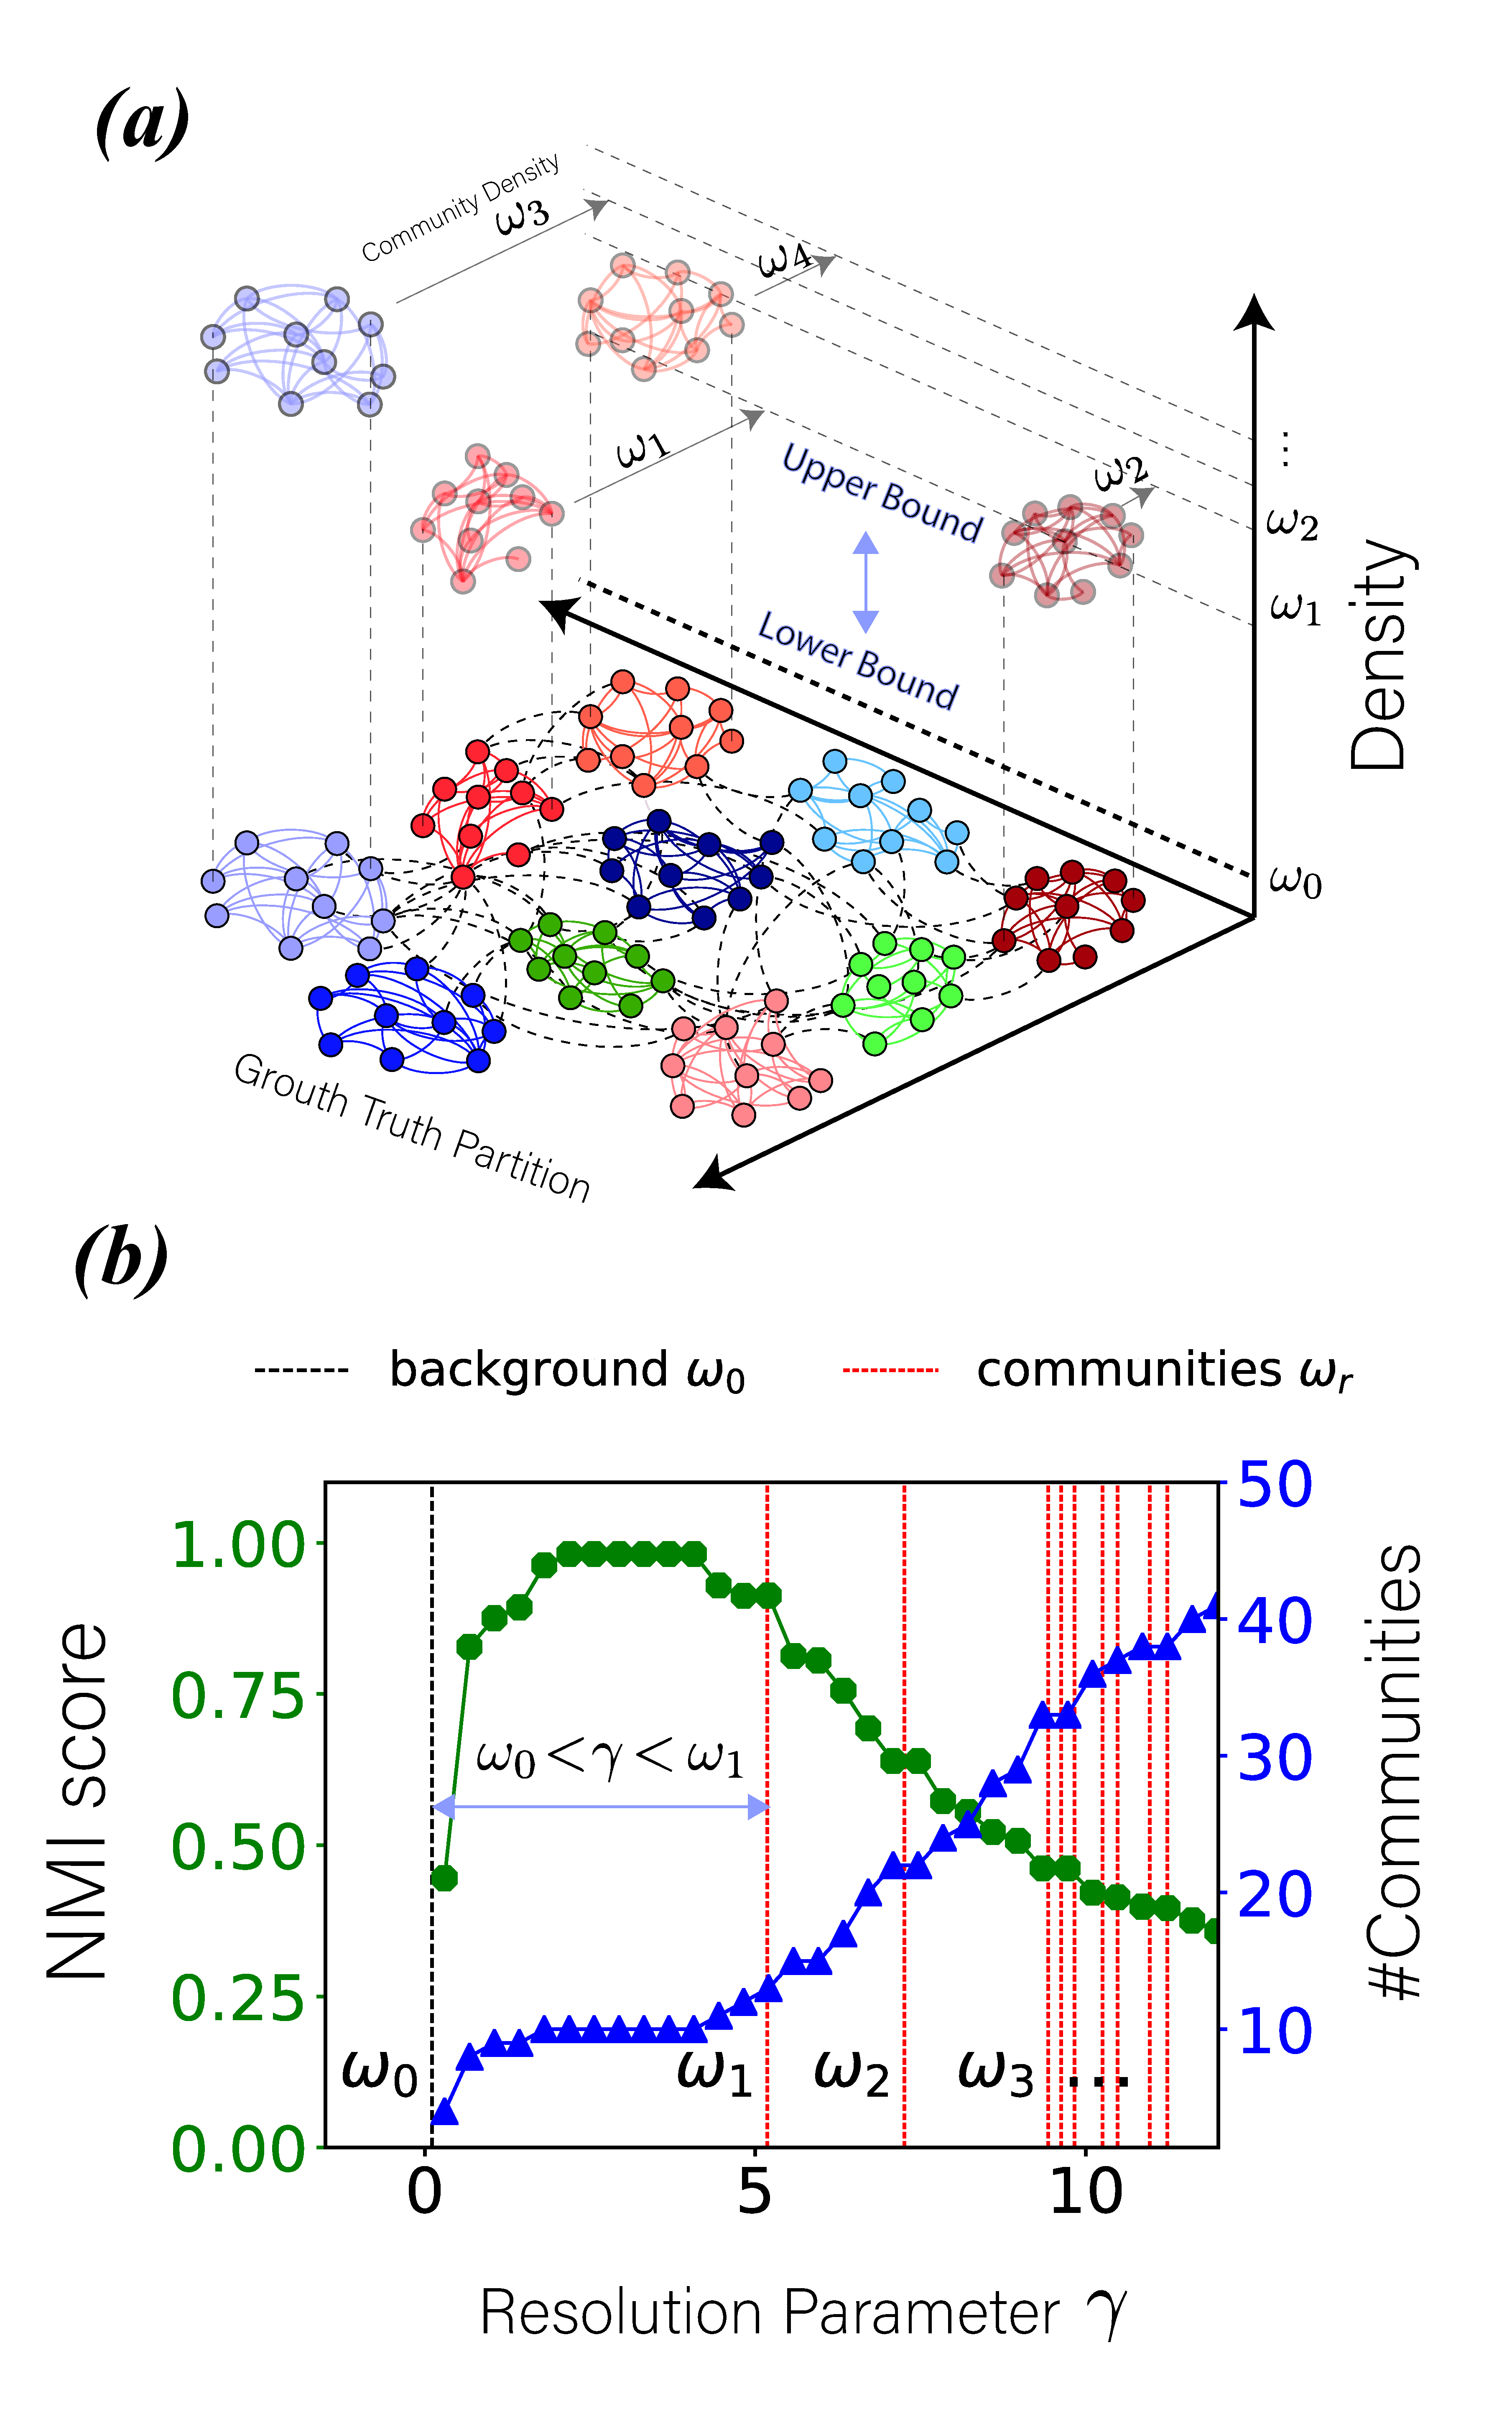
\includegraphics[width=0.6\textwidth]{img/chap2/Fig2.pdf}
    \caption{The generalized modularity performs well with resolution parameter in the interval $\gamma\in[1.8,4.2]$, matching the derived theoretical bound $\omega_0<\gamma<\omega_1$. When $\gamma$ approaches either side of the bound, the resolution scale is either higher or lower than desired. (a) Network structure and community {\it density} represented by the heights, the node color represents ground truth communities and inter-communities edges are in black dashed lines; (b) the NMI scores and the number of detected communities in relation to the resolution parameter.}
    \label{fig:gamma_error_exp}
\end{figure}

The asymptotic bounds also agree with the empirical observation made without any theoretical justification by the authors of~\cite{fenn2009dynamic,traag2013significant,mucha2010community}, that the most suitable values of the resolution parameter $\gamma$ occurs in the most stable plateaus in experiments. In addition, our results explain why \cite{newman2016equivalence} found that the statistical inference of the resolution parameter converges quickly to the desired value in small networks. It is because, once the resolution parameter falls into the range of $\omega_0<\gamma<\omega_1$, if feasible, the community detection results become stable and the inference algorithm immediately yields the final resolution parameter after this stage.

For a range of empirical networks of $n$ nodes and $m$ edges, including the Karate club network~\cite{zachary1977information}, the dolphin social network~\cite{lusseau2003bottlenose}, the network of interactions between fictional characters in the novel Les Miserables~\cite{newman2004finding} and the network of games between American college football teams in the year 2000~\cite{newman2004finding}, we compute the maximum-likelihood estimates of the background edge density $w_0$ and the lowest intra-community edge density $w_1$, fitting an extended planted partition model given the number of communities $q$ and the optimal value of $\gamma$ obtained by the statistical inference of~\cite{newman2016equivalence}. We compute the modularity maximization results with a total of $100$ different resolution parameters in the range $[0.2,3w_1/2]$ and compare these results with the communities produced with $\gamma$ from this range. The subrange which produces an NMI score higher than $90\%$ is shown in Table~\ref{tab:small_networks}. As shown in Fig.~\ref{fig:small_networks}, although these empirical networks are not generated by the extended planted partition model, the stable intervals of resolution parameter lie inside the asymptotic lower and upper bounds.

\begin{table}[]
    \centering
    \caption{The maximum-likelihood estimates of $w_0$ and $w_1$ and the interval of the resolution parameter that detects communities with NMI score larger than 90\% in a range of empirical networks of $n$ nodes and $m$ edges. The number of communities $q$ used for each network is the ground truth value generally accepted in the previous literature. The optimal $\gamma$ were published in~\cite{newman2016equivalence}.}
    \label{tab:small_networks}
    \begin{tabular}{ccccccc}
    \hline
    Network & n & m & q & $\gamma$ & $(\hat{w}_0,\hat{w}_1)$ & $90\%$ interval\\
    \hline
    Karate club & 34 & 78 &  2 & 0.78 & (0.26, 1.74) & (0.63, 1.37)\\
    Dolphin social & 62 & 159 & 2 & 0.59 & (0.12, 1.42) & (0.58, 2.0)\\
    Les Miserables & 77 & 254 & 6 & 1.36 &  (0.35, 2.83) & (1.15,  1.54)\\
    College football & 115 & 614 & 11 & 2.27 & (0.36, 5.11) & (1.78,5.61)\\
    \hline
    \end{tabular}
\end{table}


\begin{figure}[t!]
    \centering
    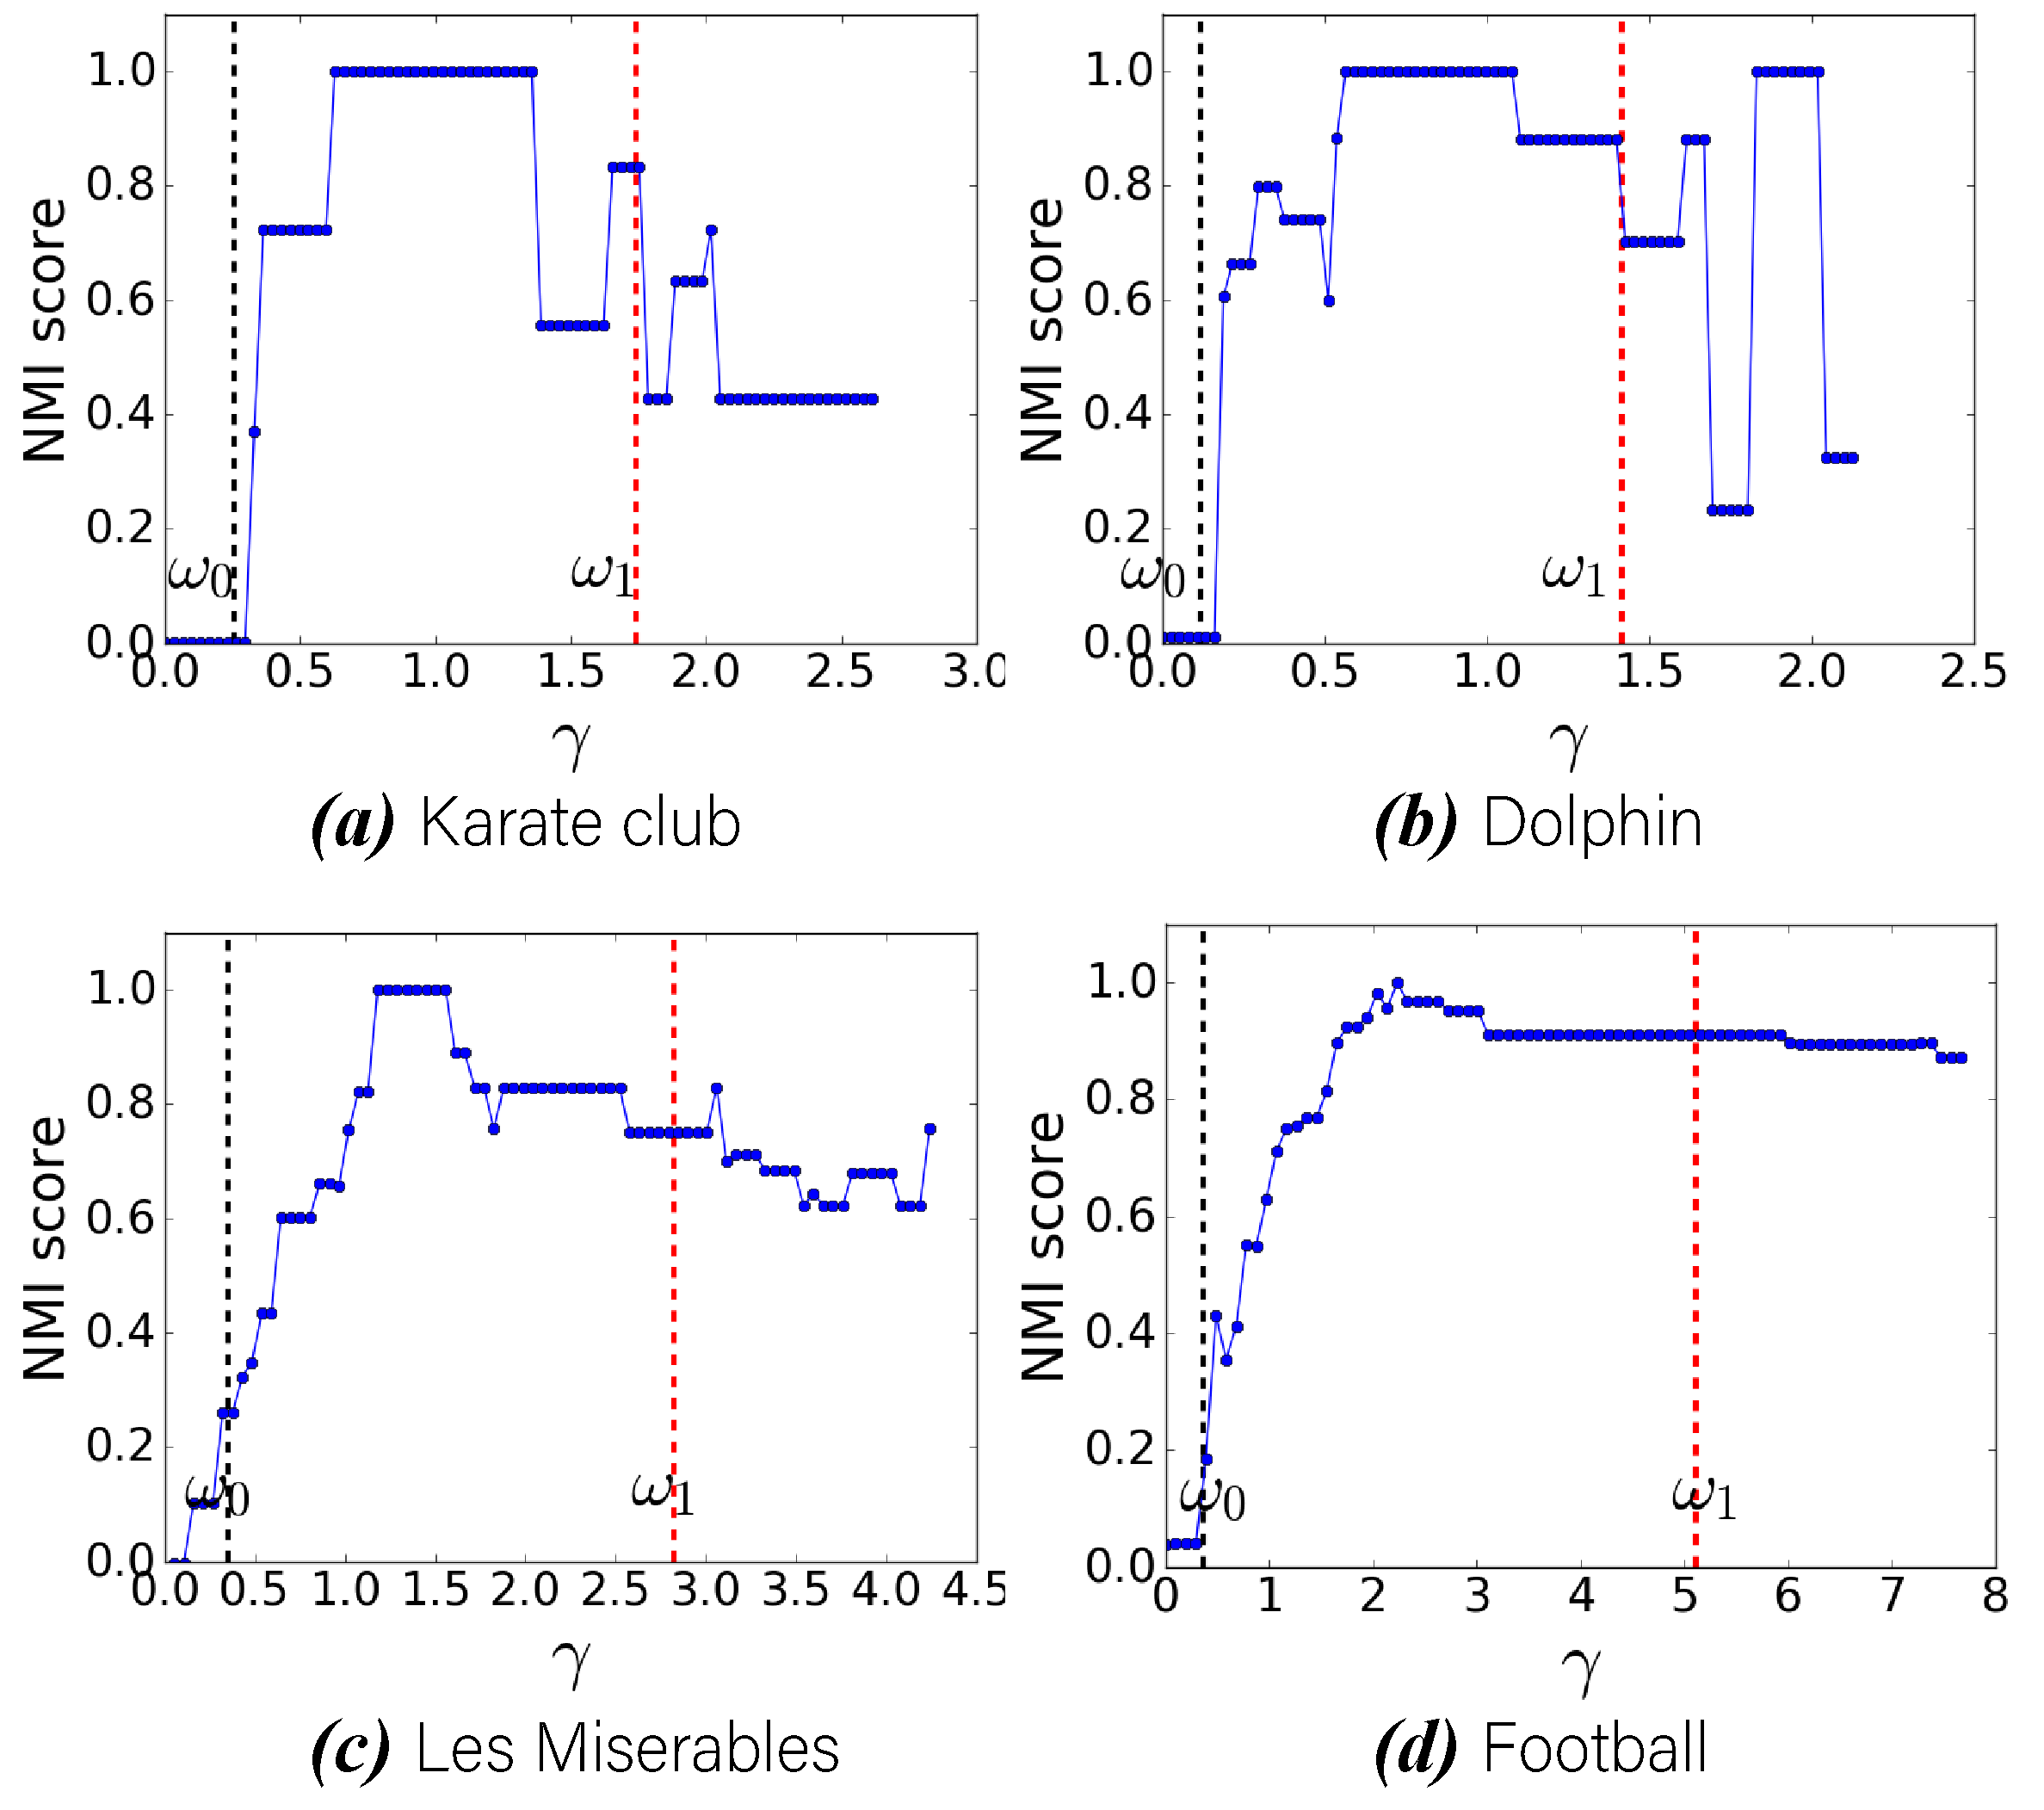
\includegraphics[width=0.8\textwidth]{img/chap2/Fig6.pdf}
    \caption{The alignment between the communities detected by generalized modularity maximization and the optimal $\gamma$ values listed in~\cite{newman2016equivalence}. Although the empirical networks are not generated by the extend planted partition model, maximizing the generalized modularity is optimal when the resolution parameter takes values that lie in the interval $[\omega_0, \omega_1]$. This phenomenon is also captured purely experimentally and without any theoretical justification in~\cite{fenn2009dynamic,mucha2010community,traag2013significant}.}
    \label{fig:small_networks}
\end{figure}


\section{Statistically significant community detection} \label{sec:2.4}
The planted partition model and its extension introduced here are all special cases of the stochastic block model. The derived asymptotic resolution bounds can be extended to the networks generated by the degree-corrected stochastic block model. Following the notations in~\cite{newman2016equivalence}, the number of edges between nodes $i$ and $j$ in the degree-corrected stochastic block model follows the Poisson distribution with the mean defined as 
\begin{equation} \label{eq:sbm_newman_definition}
\eta_{ij} = \omega_{g_i g_j} \frac{k_i k_j}{2m},
\end{equation}
where for node $l$, $g_l$ is the block assignment of this node, $k_l$ is its degree and $m$ is the total number of edges in the network.

The number of edges between two communities $r$ and $s$ in this case is approximated by 
\begin{equation} \label{eq:approx_out2}
    m_{rs} \approx \sum_{i\in r, j\in s} \omega_{rs} \frac{k_i k_j}{2m} = \omega_{rs} \frac{\kappa_r \kappa_s}{2m},
\end{equation}
where $\omega_{rs}$ denotes the (r, s)-th element of the {\it density} matrix. The number of edges between two subsets of nodes $t'$ and $t''=t - t'$ inside a community $t$ is approximated by
\begin{equation} \label{eq:approx_in2}
    m_{t't''} \approx \sum_{i\in t',j\in t''} \omega_{tt} \frac{k_i k_j}{2m} = \omega_{tt} \frac{\kappa_{t'} \kappa_{t''}}{2m},
\end{equation}
where $\omega_{tt}$ is the t-th diagonal element in the {\it density} matrix.

Using the same resolution inequality of Eq.~\ref{eq:resolution}, these approximations lead to the range
\begin{equation} \label{eq:sbm_bounds}
    \max_{r\neq s} \omega_{rs} < \gamma < \min_{r} \omega_{rr}
\end{equation}
within which a uniform $\gamma$ value avoids the resolution limit trap. 

In a network generated by the degree-corrected stochastic block model with $\omega_{rs} > \omega_{tt}$ for some $r \neq s$ and $t$, Eq.~\ref{eq:sbm_bounds} indicates that a uniform resolution parameter is not sufficient for the recovery of communities $r$, $s$ and $t$.

\begin{figure}
    \centering
    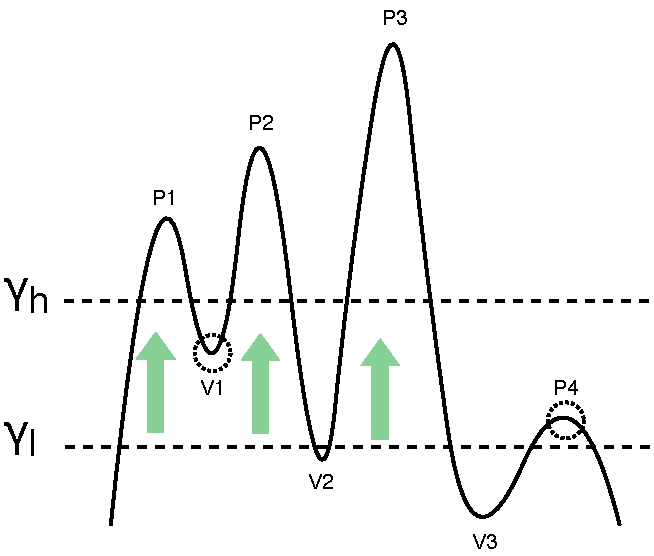
\includegraphics[width=.6\textwidth]{img/chap2/altitude.pdf}
    \caption{The plateaus problem is analogous to finding mountains that are located at different plateaus; using a single altitude either would miss the lower mountains, or would treat the higher peeks as one mountain. Specifically, when using resolution parameter $\gamma_l$, the left two high peeks P1 and P2 are considered one ``mountain" - two well-formed dense communities get merged because their inter-community edge density (illustrated by valley V1) is higher than $\gamma_l$. If we adopt a higher resolution parameter $\gamma_h$, the low peek P4 on the right gets ignored - a loose community gets split into multiple smaller clusters. Notably, this issue cannot be avoided as long as the valley V1 of the left two peeks P1, P2 is higher than the height of the right-most peek P4.}
    \label{fig:plateaus}
\end{figure}

The classical example of resolution limit trap is presented in~\cite{lancichinetti2011limits} where an undirected unweighted network contains three communities: two cliques and one ER random graph, and every two communities are connected by one single edge. Suppose each clique includes 6 nodes and the ER random graph contains 100 nodes and 956 edges. Given the three communities, the posterior estimation of the {\it density} matrix $\Omega$ of a stochastic block model, i.e., $\hat{\omega}_{rs} = \frac{2 m_{rs} m}{\kappa_r \kappa_s}$ for each communities $r$ and $s$, is
\begin{equation}
    \Omega = \begin{bmatrix}
    1.03	& 0.03  &	0.03	\\
    0.03	& 57.94 &	1.93  \\
    0.03	& 1.93  &	57.94 \\
    \end{bmatrix},
\end{equation}
where the first row and column corresponds to the random graph while the remaining rows and columns correspond to the two cliques respectively. There is no suitable resolution parameter $\gamma$ to detect three communities in this case because the {\it density} parameter for the edges between two cliques $1.93$ is larger than the {\it density} parameter for the edges inside random graph $1.03$. When applying generalized modularity maximization, adopting a resolution parameter larger than $1.93$, makes it likely that two cliques will be detected, but the random graph will get split into smaller communities. On the other hand, a resolution parameter within $[1.03, 1.93]$ preserves the random graph as one complete community, but the two clique gets merged into one community.

\begin{figure}
    \centering
    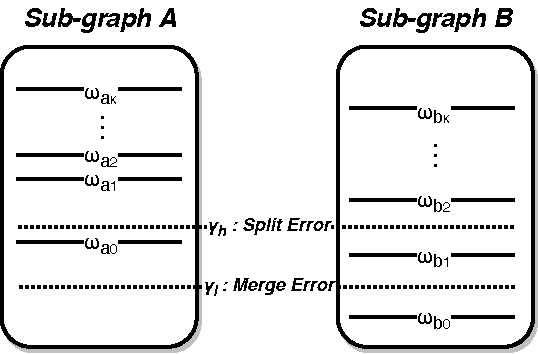
\includegraphics[width=8cm]{img/chap2/gamma_error.pdf}
    \caption{Resolution limits of the generalized modularity can be explained by the relations between the values of the density parameters of stochastic block models. Given two disjoint subgraphs A and B such that the inter-community edge density $\omega_{a0}$ in subgraph A is larger than the intra-community edge density of some community in subgraph B, no suitable resolution parameter $\gamma$ exists because Split Error and Merge Error cannot be resolved at the same time. Split Error occurs when the resolution parameter $\gamma_h$ is larger than the inter-community edge density of a subgraph A, because the community $b_1$ with the intra-community density smaller than $\gamma_h$ will be spread among multiple clusters; Merge Error occurs when the resolution parameter $\gamma_l$ is smaller than $\omega_{a0}$ so the communities in subgraph A will be merged into one community.}
    \label{fig:gamma_error}
\end{figure}

The issue is analogous to finding mountains that are located at different plateaus as shown in Fig.~\ref{fig:plateaus}; using a single altitude either would miss the lower mountains, or would treat the higher peeks as one mountain. Specifically, when using resolution parameter $\gamma_l$, the left two high peeks in Fig.~\ref{fig:plateaus} are considered one ``mountain" - two well-formed dense communities get merged. If we adopt a resolution parameter $\gamma_h$, the low peek on the right gets ignored - a loose community gets split into multiple smaller clusters. Notably, this issue cannot be avoided as long as the valley of the left two peeks is higher than the height of the right-most peek. 

More formally, given the {\it density} matrix of a degree-corrected stochastic block model and a set of communities $S=\{r\}$, the sub-matrix $\Omega_{S,S}$ formed by the rows and columns in $r\in S$ corresponds to a subgraph in the networks. Suppose subgraphs A and B have the inter-communities {\it density} parameter $\omega_{w_{a0}}$ and $\omega_{w_{b0}}$ respectively. In Fig.~\ref{fig:gamma_error}, using $\gamma_h$ causes {\it Split Error} which splits some community with $\omega_{b1} < \gamma_h$ in  B while using $\gamma_l$ causes {\it Merge Error} which merges all communities in subgraph A.

This problem is more common in large networks than in small ones, as large networks are more likely to have inhomogeneous subgraphs in different regions. For this reason, a uniform resolution limit parameter is not sufficient to resolve communities located at different ``plateaus''. Motivated by this ``plateaus'' phenomenon, we propose a multi-scale community detection algorithm which gradually increases the resolution parameter to detect community in local subgraphs.

We propose an agglomerative heuristic algorithm which recursively divides the network into subgraphs to detect communities at different scales. At each level of recursion, the algorithm applies a resolution parameter $\gamma < 1$ in attempt to avoid inappropriately splitting of loose communities. But it is likely to merge inappropriately small well-formed communities into large ones. Therefore, the discovered subgraphs are then passed to the next level of recursion to further detect communities with higher edge {\it density} parameter. This idea is illustrated in Fig.~\ref{fig:plateaus} where the peeks located at a higher plateaus need a high altitude $\gamma_h$ for each to have its own community.

The remaining challenge is to determine when to terminate the recursion. As the network breaks into smaller subgraphs recursively, the algorithm should stop when there is actually only one community in each subgraph. Indeed, one can always increase the resolution parameter to detect higher resolution communities in this subgraph. But it does not mean the current subgraph always contains community structures. For instance, a Erdos-Renyi random graph~\cite{erdHos1960evolution} can be partitioned into communities as long as the resolution parameter is high enough. However, we do not claim that Erdos-Renyi graph has community structures.

To ensure the detected communities are meaningful, we apply a {\bf hypothesis testing framework} to ensure the significance of the partition. The \textit{null} model $H_0$ here is defined as a simplified version of the degree-corrected planted partition model in which only one community exists, and the more general, nesting alternative $H_1$ is defined as the degree-corrected planted partition model whose log-likelihood is represented by Eq.~\ref{eq:modularity} given the current partition $\bf g$. 

The {\it null} model $H_0$ here is a special case of the degree-corrected planted partition model~\cite{newman2016equivalence}. The number of edges between nodes $i$ and $j$ follows the Poisson distribution with mean
\begin{equation}
    \eta_{ij} = \omega \frac{k_i k_j}{2m},
\end{equation}
where $\omega$ is a model parameter independent of the block assignments. Hence, we can consider this model as the degree-corrected planted partition model with only one community and the $\omega$ is the corresponding {\it density} parameter. The log-likelihood of this \textit{null} model can be simplified from Eq.~\ref{eq:ll} to the following
\begin{equation} 
\begin{split}
    \log P_{\text{null}}({\bf A}|\omega) &= \frac{1}{2} \sum_{ij} \left[ A_{ij} \log \left(\omega\frac{k_i k_j}{2m} \right) - \omega\frac{k_i k_j}{2m} \right] \\
                           &= m \left(\log w - w\right) + \sum_i k_i \log k_i - m \log \left(2m\right) .
\end{split}
\end{equation}
Taking the first-order derivative of the log-likelihood above over $\omega$, it is easy to obtain the maximum likelihood estimate $\hat{\omega} = 1$, hence the posterior log-likelihood can be written as
\begin{equation} \label{eq:null_ll}
\log P_{\text{null}}({\bf A}) = - m + D,
\end{equation}
where $D$ is the constant term given in Eq.~\ref{eq:BCD}, which actually can be cancelled eventually in the test statistic as shown below.

It is worth noting that the {\it null} model defined here is similar to the configuration model~\cite{molloy1995critical}, but they are not exactly equivalent. The configuration model~\cite{molloy1995critical} is a random graph model which assumes the edges are placed randomly between the nodes, while the degree of every node after such randomization is equal to the corresponding value in the original network. The network generation process in the configuration model can be understood as follows: The degrees of the vertices are represented as the number of half-links or stubs. These stubs are randomly paired with each other to create the edges. Hence, the configuration model produces an ensemble of graphs with the exact degree sequence as in the original network. The number of edges between nodes $i$ and $j$ averaged over the ensemble of graphs generated in this way is equal to $\frac{k_i k_j}{2m}$ where $m$ is again the total number of edges in the original network and $k_l$ is the degree of node $l$. In the {\it null} model defined here, when the $\omega$ parameter takes the MLE value $\hat{\omega} = 1$, the expected number of edges between nodes $i$ and $j$ is also $\frac{k_i k_j}{2m}$. But this {\it null} model allows multi-edges and self-edges (edges connecting a node to itself). The expected degree of the node $i$ in the {\it null} model is $\sum_j \frac{k_i k_j}{2m} = k_i \frac{\sum_j k_j}{2m} = k_i$.

In general, the alternative model $H_1$ splitting a network into multiple communities should fit better to the observed network than the {\it null} model does because the alternative model involves many more model parameters. The log-likelihood of the degree-corrected planted partition model, $\log P_{\text{pp}}$, is supposed to be higher than the log-likelihood of the {\it null} model, $\log P_{\text{null}}$ as defined in Eq.~\ref{eq:modularity}. Therefore, we use the log-likelihood ratio statistic (LLR)~\cite{ghosh1984asymptotic} as a test statistic to measure their difference. Given a partition of the network $\bf g$, the LLR is written as
\begin{equation} \label{eq:-2ll}
    \begin{split}
    \Lambda_{\bf g} &= -2 \log \frac{P_{\text{null}}({\bf A})}{P_{\text{pp}}({\bf A};\hat{\Omega}_{\bf g},{\bf g})} \\
                      &= 2 \left[ \log P_{\text{pp}} \left( {\bf A};\hat{\Omega}_{\bf g},{\bf g} \right) - \log P_{\text{null}} \left( {\bf A} \right) \right],
    \end{split}
\end{equation}
where $\hat{\Omega}$ is the posterior most-likely {\it density} parameters estimated from the given partition $\bf g$. The log-likelihood ratio statistic is equal to twice the difference between the log-likelihood of two models, $\log P_{\text{pp}}$ and $\log P_{\text{null}}$. 

It is worth noting that the partition $\bf g$ is detected by the generalized modularity maximization and used to compute $\log P_{\text{pp}}({\bf A};\hat{\Omega}_{\bf g},{\bf g})$ in our case. A low resolution parameter $\gamma$ value is used for the generalized modularity maximization here because it is likely to result in a small number of communities, limiting the number of parameters in the alternative model $H_1$. Hence, it prevents the $H_1$ model from overfitting. Most importantly, this choice avoids the multiple re-estimation of $\gamma$, which is computationally expensive because it needs to maximize the generalized modularity over the same network many times with different $\gamma$ values~\cite{newman2016equivalence}. In practice, we choose a $\gamma$ value slightly smaller than $1$ in the experiments.

Plugging the specific expression of the log-likelihoods of these two competing models, Eq.~\ref{eq:modularity} and Eq.~\ref{eq:null_ll}, into Eq.~\ref{eq:-2ll} yields the test statistic in a simple form
\begin{equation} 
    \begin{split}
    \Lambda_{\bf g} &= 2 \left[ B \cdot Q \left(\hat{\gamma}, {\bf g} \right) + C + m \right] \\
        &= m \left[\log \frac{\hat{\omega}_1}{\hat{\omega}_0} \cdot Q \left(\hat{\gamma}, {\bf g} \right) + \left(\log \hat{\omega}_0 - \hat{\omega}_0 \right) + 1 \right],
    \end{split}
\end{equation}
where the constants $B$ and $C$ are defined in Eq.~\ref{eq:BCD} but the parameters $\omega_1$ and $\omega_0$ take their MLE values, and $Q(\hat{\gamma}, {\bf g})$ is the generalized modularity of the partition $\bf g$ with a resolution parameter $\hat{\gamma}$ defined by posterior maximum likelihood estimate, $\hat{\omega}_0$ and $\hat{\omega}_1$ are the {\it density} parameters obtained by the posterior maximum likelihood estimation given partition $\bf g$. With $\hat{\gamma}$ and ${\bf g}$, it takes $O(m)$ time to compute $Q(\hat{\gamma}, {\bf g})$ where $m$ is the total number of edges in the network. Given the modularity $Q(\hat{\gamma}, {\bf g})$, the LLR test statistic can be computed in constant time.

In general, the alternative model $H_1$ splitting a network into multiple communities should perform at least as well as the \textit{null} model, because the alternative model involves many more model parameters, i.e. the {\it density} matrix $\Omega$. $H_1$ is accepted when the fit is significantly better, i.e. $\Lambda_{\bf g}$ is large enough. Such significance is measured by the \textit{p-value} of $\Lambda_{\bf g}$ defined as
\begin{equation}
    \textit{p-value} = P [\Lambda_{\text{null}} > \Lambda_{\bf g}],
\end{equation}
where $\Lambda_{\text{null}}$ is the corresponding log-likelihood value under the {\it null} hypothesis, which can be computed numerically by sampling a series of \textit{null} networks generated by the {\it null} model. If the {\it p-value} is smaller than the significance level, the {\it null} hypothesis is rejected and the algorithm does hypothesis testing on the resulting communities; Otherwise, the algorithm returns the current subgraph as one single community and stops the current recursion branch. The hypothesis testing procedure is summarized below:
\begin{itemize}
    \item Maximize the generalized modularity with a predefined $\gamma < 1$ to obtain partition $\bf g$.
    \item Estimate the {\it density} parameters $\hat{\Omega} = \{\hat{\omega}_0, \hat{\omega}_1\}$ of degree-corrected planted partition model by Eq.~\ref{eq:update_omega} and the corresponding resolution parameter $\bf \hat{\gamma}$ by Eq.~\ref{eq:gamma_mle}. Then compute the generalized modularity $Q(\hat{\gamma}, {\bf g})$ so the log-likelihood ratio test $\Lambda_{\bf g}$ can be obtained.
    \item Generate a series of \textit{null} networks via the {\it null} model. Compute $\Lambda_{\text{null}}$ for each \textit{null} network, output the fraction of $\Lambda_{\text{null}}$s which are larger than $\Lambda_{\bf g}$ as the \textit{p-value}.
    \item If the {\it p-value} is smaller than the significance level, reject $H_0$ and continue partitioning the subgraph. Otherwise, accept $H_0$ and return the current subgraph as a community.
\end{itemize}

It is worth noting that, according to the Wilks' theorem~\cite{wilks1938large}, when the sample size, i.e. the number of sampled {\it null} networks, approaches infinity, the log-likelihood ratio test statistic as defined in the form of Eq.~\ref{eq:-2ll} is asymptotically chi-squared distributed when the $H_0$ hold true. We can actually avoid enumerating a large set of {\it null} networks to calculate the {\it p-value}. Instead, given $\Lambda_{\bf g}$, the {\it p-value} can be directly approximated using the chi-squared distribution. However, in practice, the quality of $\bf g$ also influence the test statistic $\Lambda_{g}$. We observed that modularity maximization over a larger network often detects better $\bf g$ than over smaller ones, resulting in large test statistic $\Lambda_{g}$. Therefore, we find it more computationally efficient to terminate the current recursion branch when $\Lambda_{\bf g} < \tau * n_{sub}$ where $\tau$ is a constant value and $n_{sub}$ is the number of nodes in the currently considered subgraph. The accurate calculation of {\it p-value} by sampling {\it null} networks can still be used for relatively small network when needed.

To evaluate the performance of the proposed multi-scale community detection algorithm, we compare it with the state-of-art greedy modularity maximization algorithm, Fast Greedy~\cite{clauset2004finding}, on several real and synthetic networks. For the networks with pre-defined ground truth communities, the quality of the detected communities are evaluated by the Normalized Mutual Information (NMI) and Adjusted Rand Index (ARI) metrics which requires ground truth communities. Besides, we also measure the distribution of the community sizes which usually reflects the resolution limits problem because modularity maximization either combines smaller well-formed communities into bigger ones or splits larger well-formed communities into smaller ones. The definition of the two quality metrics mentioned above are given below.

One of the standard sources of community structures for the evaluation of community detection algorithms is the LFR benchmark~\cite{lancichinetti2008benchmark} which generates networks based on a set of pre-defined ground truth communities. In so generated networks, both the degree and community size distributions follow the power law. The main benefit of using LFR benchmark is that the ground truth communities are known. The generated networks vary with the following three parameters: $\gamma$ which is an exponent of the node degree in the power law distribution, $\beta$ which is an exponent of the community size in the power law distribution, and $\mu$ which is the {\it density} parameter that defines the fraction of all edges which have both endpoints inside the same community. 

In our experiments, the networks generated by the LFR benchmarks have the average node degree of 9.3 and the numbers of nodes ranging from 6,000 to 11,000. The exponents $\gamma$ and $\beta$ are set to 3.0 and 2.0 respectively and the {\it density} parameter $\mu$ is equal to 0.25. We evaluate the modularity maximization performance using the Fast Greedy algorithm~\cite{clauset2004finding}. The results are measured by the NMI and ARI metrics as shown in Table~\ref{tab:1}. The number of communities as a function of their sizes is plotted in Fig.~\ref{fig:5}. One notable difference between the community detection results is that the modularity maximization merges smaller communities into larger ones so there is fewer small communities in the results than in the ground truth. This is the main reason why modularity maximization does not perform as well as the proposed multi-scale community detection which recursively divides a large community into small ones until the probability that it contains communities becomes statistically insignificant.

\begin{table}[]
\centering
\caption{Performance of multi-scale community detection compared to the Fast Greedy~\cite{clauset2004finding} modularity maximization algorithm on the LFR benchmark networks. Note large increase in value of metrics for multi-scale algorithm, at least 38\% for NMI and 240\% for ARI}
\label{tab:1}
\begin{tabular}{ccccc}
\hline
\multirow{2}{*}{\#Nodes} & \multirow{2}{*}{\#Edges} & \multirow{2}{*}{Metric} & \multirow{2}{*}{Fast Greedy} & \multirow{2}{*}{Multi-scale} \\
                  &                   &                  &            &                           \\
\hline

\multirow{2}{*}{5000} & \multirow{2}{*}{23436} & ARI     &  0.20368   &  0.69378                \\
                  &                   &          NMI     &  0.60266   &  0.83706                         \\
\multirow{2}{*}{7000} & \multirow{2}{*}{31546} & ARI     &  0.12377   &  0.71148                \\
                  &                   &          NMI     &  0.62044   &  0.87240                         \\
\multirow{2}{*}{9000} & \multirow{2}{*}{41595} & ARI     &  0.11038   &  0.74156               \\
&                   &          NMI     &  0.59043   &  0.87355                        \\
\multirow{2}{*}{11000} & \multirow{2}{*}{51430} & ARI     &  0.12701   &  0.75043               \\
&                   &          NMI     &  0.56224   &  0.86722              \\          
\hline
\end{tabular}
\end{table}

\begin{figure}[!ht]
    \centering
    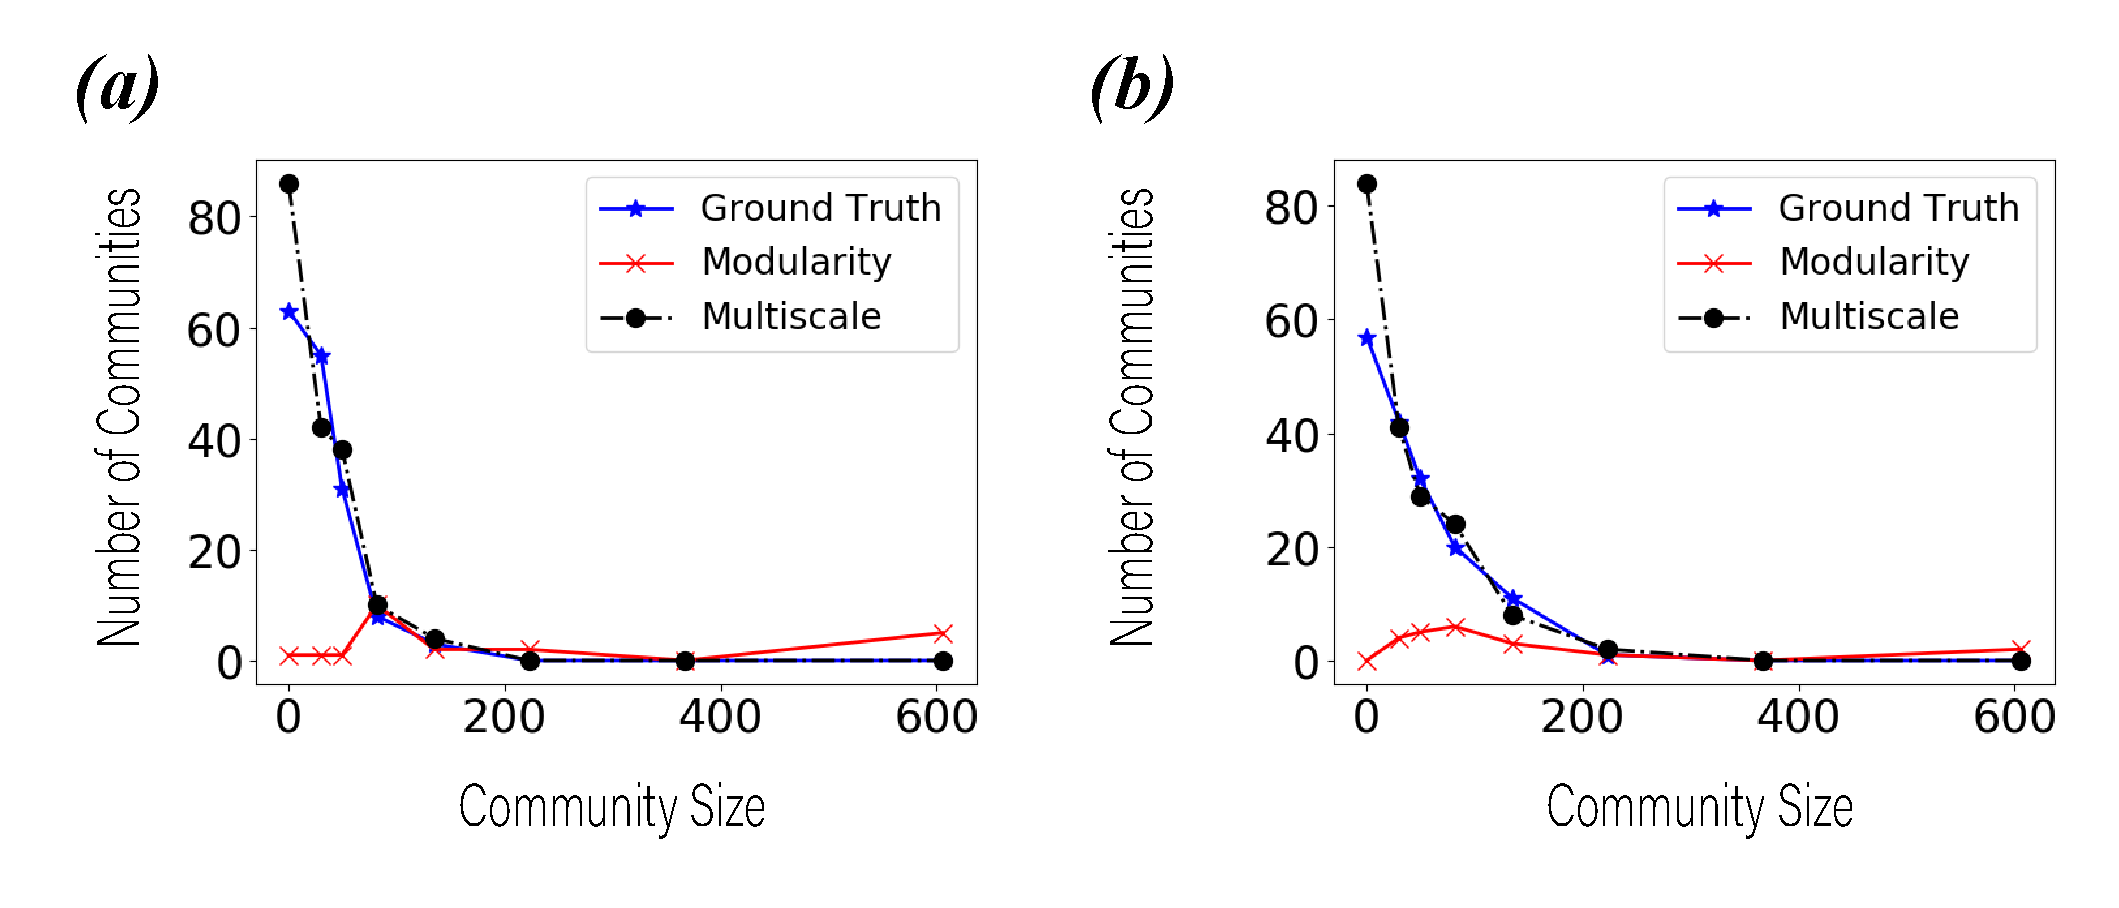
\includegraphics[width=0.9\textwidth]{img/chap2/Fig5.pdf}
    \caption{Histogram of detected community sizes using the state-of-the-art modularity maximization algorithm, Fast Greedy~\cite{clauset2004finding}, and the proposed multi-scale modularity maximization approach. This approach detects fewer small communities and more large communities compared to the ground truth due to the resolution limit problem. In contrast, the multi-scale approach detects the numbers of communities of over wider range of sizes. (a) LFR benchmark network with 7000 nodes (b) LFR benchmark network with 11,000 nodes.}
    \label{fig:5}
\end{figure}

The American college football network~\cite{evans2010clique} consists of 115 nodes representing college football teams playing in a league with 11 conferences. Every edge in the American college football network denotes the positive number of games played by two teams in the year 2000 season. According to~\cite{evans2010clique}, each of the 11 college football conferences active at the time gets identified as one community because teams within a conference play more frequently with each other than with teams from other conferences. There are 8 independent teams (not members of any conference), each forming a single community. 

\begin{figure}
    \centering
    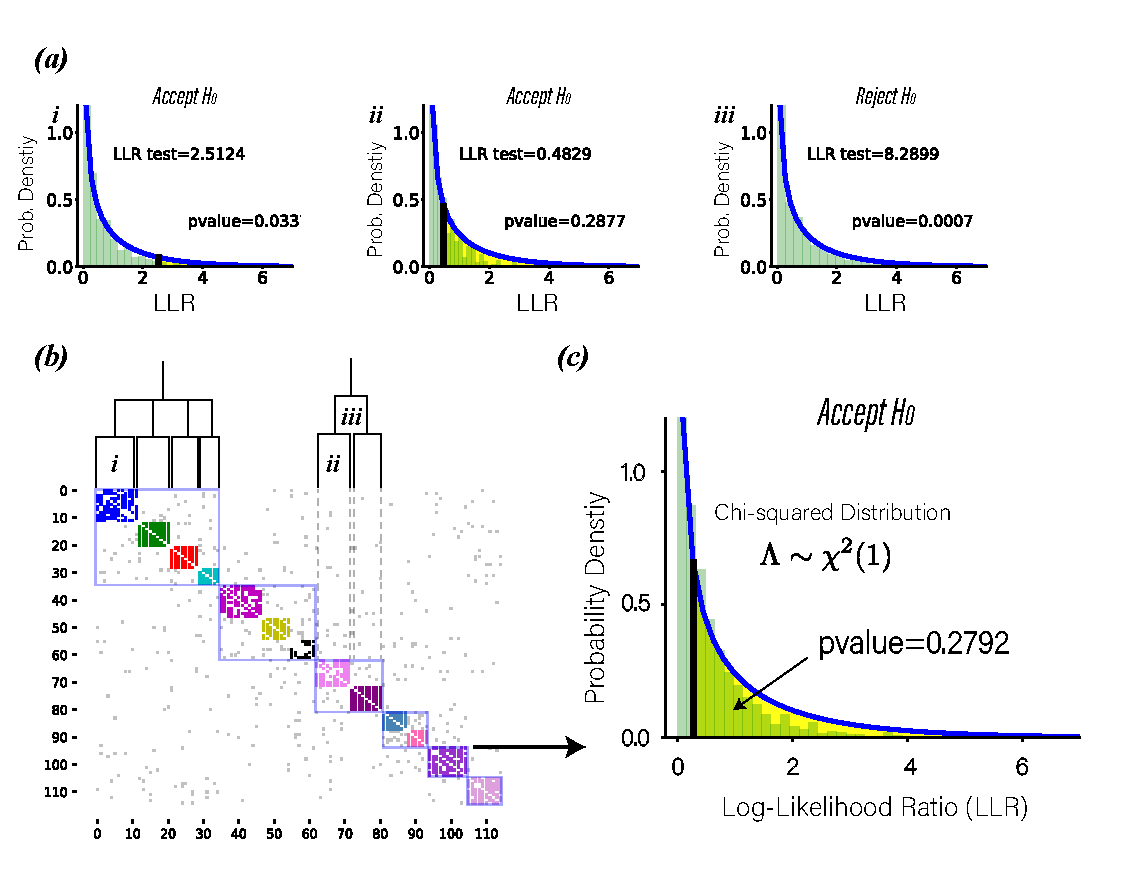
\includegraphics[width=0.8\textwidth]{img/chap2/football.pdf}
    \caption{Illustration of the multi-scale community detection in the American college football network~\cite{evans2010clique}. (a) Three different hypothesis testing cases are: in cases (i) and (ii) the {\it null} hypothesis is accepted because statistically significant community has been found while in case (iii) the {\it null} hypothesis is rejected because the subgraph actually consists of two smaller communities. (b) The edge matrix where each dot indicates the one edge. Different colors define final communities detected by multi-scale community detection, while the rectangles show the communities detected at the first level. (c) A well-formed community passes the statistical significance test at the first level, and thus avoids further splitting. The green histogram shows the distribution by sampling {\it null} networks, the blue curve indicate the chi-squared distribution, and the size of the yellow area corresponds to the {\it p-value}.}
    \label{fig:football_pvalues}
\end{figure}



Fig.~\ref{fig:football_pvalues} illustrates the steps of significance testing of the communities at two different levels. The generalized modularity with a predefined resolution parameter $\gamma=0.9$ is maximized to obtain partitions. As shown in Fig.~\ref{fig:football_pvalues}(b), at the first level, the networks is partitioned into 6 communities covered by the rectangles - some correspond to the well-formed ones because their community {\it densities} are larger than the resolution bound; the others, however, consist of multiple well-formed but smaller communities, each represented by an unique color. Then, the algorithm does hypothesis testing given the partition at the first level - it estimates the corresponding posterior maximum-likelihood estimates of {\it density} parameters $\hat{\Omega}$ and evaluate the log-likelihood ratio test $\Lambda_{\bf g}$. Then, the algorithm generates a series of \textit{null} networks via the configuration model, given the degree sequence of the network. Since the {\it p-value} is smaller than the significance level $0.01$ chosen here, which is typically used for such tests, we reject the {\it null} hypothesis $H_0$ and continue partitioning the each of the 6 communities. At the second level, each individual community is treated as a subgraph, and the same generalized modularity maximization procedure is repeated on each of them again.
The second community at the bottom right corner has a high community {\it density}, thus, the {\it null} hypothesis gets accepted with high p-value of $0.2792$, in case (i) and similarly in case (ii).
However, in case (iii), as shown in Fig.~\ref{fig:football_pvalues}(a)(iii), the {\it p-value} $0.0007$ is much smaller than the significance level of $0.01$ used here. Therefore, the multi-scale community detection algorithm rejects $H_0$ and further splits that ill-formed community into two smaller ones. The modularity maximization conducted by Fast Greedy obtains 6 communities similar to the ones covered by the six rectangles in Fig.~\ref{fig:football_pvalues}(c) and it obtains a NMI score of $0.5572$. The proposed multi-scale community detection algorithm finds $13$ communities, achieving the NMI scores of $0.8728$.


\section{Regularized Stochastic Block Model} \label{sec:2.5}
As defined in previous literatures~\cite{newman2004finding,fortunato2010community}, the assortative structures correspond to the traditional community structures, nodes are more frequently connected with each other inside communities than with the rest of the network. The disasortative structures do not satisfy this condition. For example, the core-periphery structures~\cite{borgatti2000models} divides the networks nodes into the core part, where nodes are often the hubs of the networks, and the periphery part, where nodes of low-degree connect to the core nodes. This is an advantage of the degree-corrected stochastic block model because it allows the discovery of the structures with different mixing patterns. However, when searching for the weak assortative community structures, the inference algorithm may still return the disassortative structure\cite{decelle2011asymptotic} instead.

We generate synthetic networks using the degree-corrected stochastic block model with a block assignment $\{g_i\}$ and the parameters $\omega_{rs}$ chosen for the assortative communities as follows
\begin{equation} \label{eq:synthetic}
\omega_{rs}=
    \begin{cases}
    &\gamma \omega_{0} \quad \quad  \text{ if  } r=s,\\
    &\omega_{0} \quad \quad \quad  \text{if  } r\neq s.
    \end{cases}
\end{equation}
where a large value of $\gamma$ results in strong community structure while $\omega_{0}$ controls the sparsity of the network. The degree sequence is drawn from a power-law distribution with exponent $2.5$, and the block assignments are randomly assigned, but each block is of the same size.

\begin{figure*}[!htb]
\centering
\begin{subfigure}{.5\textwidth} 
\centering
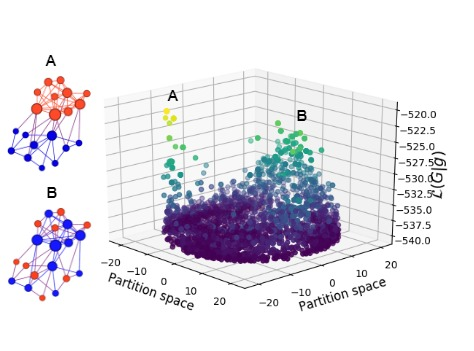
\includegraphics[width=.99\linewidth]{img/chap2/opt_figure_dcsbm.jpg}
\caption{Local optima of log-likelihood}
\end{subfigure}
\begin{subfigure}{.45\textwidth} 
\centering
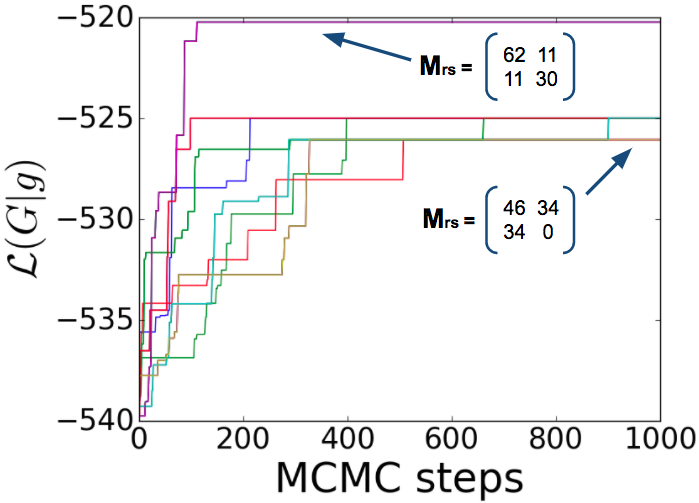
\includegraphics[width=.99\linewidth]{img/chap2/dcsbm_converge2.png}
\caption{Convergence}
\end{subfigure}
\caption{The convergence of 20 Markov Chain Monte Carlo (MCMC) trials for the degree-corrected stochastic block model. The local optimum $A$ found by MCMC represents the assortative communities, whereas there are other local optima representing disassortative structures such as point B. \textbf{(a)} Multiple locally optimal partitions discovered by the MCMC inference for degree-corrected stochastic block model; \textbf{(b)} 2 out of the 20 MCMC trials find the most likely and sought-after assortative partition, while the other trials get trapped at the local optima. The matrix $M_{rs}$ indicates the number of edges between every pair of blocks.}
\label{fig:dcsbm_3dscatter}
\end{figure*}

Given the synthetic networks produced by the degree-corrected stochastic block model, we infer the block assignment $\{g_i\}$, recovering the parameters used for its generation. Specifically, the number of communities is set as two for both the generation and recovery. To generate samples, the degree-corrected stochastic block model uses $\omega_{0}=0.01$ and $\gamma=10$. Each of the two blocks contains $10$ nodes. We scatter the sampled partitions on the x-y plane in Figure~\ref{fig:dcsbm_3dscatter} and the z-axis indicates the log-likelihood of the corresponding partitions. We adapt the Markov chain Monte Carlo (MCMC) algorithm~\cite{nasrabadi2007pattern,peixoto2014efficient} to infer the block assignment of the stochastic block model and its extensions. The MCMC algorithm~\cite{peixoto2014efficient} samples the distribution of all possible block assignments in the network partitions space. For each trail, the algorithm starts from a random partition and iteratively, with certain probability, traverse to an adjacent partition. An entire MCMC sweep of all nodes in the network requires $O(E)$ operations where $E$ is the number of edges in the networks~\cite{peixoto2014efficient}. The mixing time of the MCMC algorithm depends on the specific input network and the starting point. The details of the MCMC algorithm are discussed in the Supplementary Information.

Figure~\ref{fig:dcsbm_3dscatter} shows the existence of multiple local optima in the log-likelihood of degree-corrected stochastic block model. The inference process finds three local optima here: (i) partition A which corresponds to the assortative structure matching the ground truth block assignment used for its generation; (ii) partition B which corresponds to a disassortative structure; and (iii) another disassortative partition which is not explicitly marked in the Figure~\ref{fig:dcsbm_3dscatter}(a). Under the degree-corrected stochastic block model, the MCMC inference starting from random initial partition finds the most suitable partition A in only 2 out of 20 trials, whereas the other attempts are trapped at the local optima as shown in Figure~\ref{fig:dcsbm_3dscatter}(b).

Since there are multiple local optima in the log-likelihood of the degree-corrected stochastic block model, the inference algorithm may converge to any of them nondeterministically. Specifically, the type of the discovered structure depends on the trial starting point and inference algorithm parameters. To avoid such nondeterministic outcomes, we introduce a novel approach called Regularized Stochastic Block Model (RSBM) applicable to any inference algorithm. RSBM constrains nodes' internal degree ratios, each of which is defined in the objective function as the fraction of a node's neighbors inside the same community. The resulting algorithm reliably finds assortative or disassortative structures as directed by the value of a single parameter. 
% The resulting partition inferred by MCMC algorithm quickly converges to the desired assortative structures when they exist in the sparse networks. In addition, the resulting partition of our model can be used as the initial block assignment for the inference of degree-corrected stochastic block model, which has been shown experimentally to escape the disassortative structure in sparse networks.

%\subsection{Regularized stochastic block model}
%The maximum likelihood estimates of $\theta_l$ is $\hat{\theta}_l = \frac{k_l}{\kappa_{g_l}}$ where $k_i$ is the degree of node $i$ and $\kappa_r$ is the sum of degrees of the nodes in the community (block) $r$, while the maximum likelihood estimate of $\omega_{rs}$ is equal to the number of edges between communities $r$ and $s$, i.e.  $\hat{\omega}_{rs} = m_{rs}$. Therefore, for a node $i$, the expected node degree in degree-corrected stochastic block model is $\sum_j \lambda_{ij} = $

We extend the formulation of the expected number of edges between nodes $i$ and $j$, determined by the \textit{Poisson} rate $\lambda_{ij}$, in the degree-corrected stochastic block model by defining it as
\begin{equation} \label{eq:theta}
    \lambda_{ij} = 
    \begin{cases}  \omega_{g_i,g_j} I_i I_j    & \mbox{if} \quad g_i=g_j\\
                                 \omega_{g_i,g_j} O_i O_j  & \mbox{otherwise}
    \end{cases}
\end{equation}
where any node $l$ has two associated parameters $I_l$ and $O_l$. Given Eq.~\ref{eq:ll}, the log-likelihood of generating graph $G$ by this regularized stochastic block model can be written as
%\begin{equation}
%    P(G|{\bf g,\omega, I, O}) \propto \prod_{ij} \lambda_{ij}^{A_{ij}} \exp(-\lambda_{ij})
%\end{equation}
%Using Eq.~\ref{eq:theta}, the log-likelihood can be written as
\begin{align} \label{eq:logl_IO}
    \OP(G|{\bf g,\omega, I, O})  = 2\sum_i \Big( k_i^+ \log I_i + k_i^- \log O_i \Big) + \sum_{rs} m_{rs} \log \omega_{rs} - \omega_{rs} \Lambda_{rs} 
\end{align}
where $k_i^+$ is the number of neighbors of node $i$ which are inside the same block given the block assignment $\bf g$ and $k_i^- = k_i - k_i^+$. Thus, we get  
\begin{align}
   \Lambda_{rs} = \begin{cases}  (\sum_{i \in r} I_i)^2   & \mbox{if } r=s \\ 
 \sum_{i \in r} O_{i}  \sum_{i \in s} O_{i} & \mbox{if } r\neq s \end{cases} 
\end{align}
To simplify, we write $i\in r$ if $g_i = r$. For block assignment $\bf g$, the maximum-likelihood values of $\omega_{rs}$ are
\begin{equation} \label{eq:mle_omega}
    \hat{\omega}_{rs} = \frac{m_{rs}}{\Lambda_{rs}}
\end{equation}
Dropping the constants and substituting using Eq.~\ref{eq:logl_IO}, we obtain
\begin{align} \label{eq:important}
    \OP(A|{\bf g,I,O})
    &=  \sum_{rs} m_{rs} \log \frac{m_{rs}}{\Lambda_{rs}} + 2\sum_i \Big( k_i^+ \log I_i + k_i^- \log O_i \Big) 
\end{align}

Note that if we set $I_i = O_i = 1$ here, the log-likelihood above reduces to the definition of standard stochastic block model with $\Lambda_{rs} = n_r n_s$ which is exactly the product of the sizes of two blocks $r$ and $s$. When $I_i = O_i = k_i$, the second sum on the right hand side (RHS) becomes irrelevant to the maximum likelihood estimation (MLE) result. Hence, the log-likelihood reduces to the definition of degree-corrected stochastic block model in Eq.~\ref{eq:important} with $\Lambda_{rs} = \kappa_r \kappa_s$, i.e., the product of the sums of degrees of nodes in two blocks $r$ and $s$. Hence, by introducing two sets of parameters ${\bf I} = \{I_i\}$ and ${\bf O} = \{O_i\}$ in the edge probability, we obtain a more generalized definition of stochastic block model here.

%\subsection{Regularization by prior in-degree ratios }
For alternative formulation of our model, we define the prior in-degree ratio $f_i = I_i / (I_i + O_i)$ and $\theta_i = I_i + O_i$ for each node $i$. By rewriting the second summation on the RHS of Eq.~\ref{eq:important}, we get 
%\begin{align}
%\sum_i k_i^+ \log I_i + k_i^- \log O_i &= \sum_i k_i \Big( \frac{k_i^+}{k_i} \log f_i + \frac{k_i^-}{k_i} \log (1-f_i) + \log \theta_i \Big)\\
%    &= - \sum_i k_i H(\frac{k_i^+}{k_i},f_i) + \sum_i k_i \log \theta_i \label{eq:last_eli}
%\end{align}
%where $H(p,q)$ denotes the cross entropy between two probability distributions $p$ and $q$. With this simplification, the log-likelihood has an alternative form
\begin{align} \label{eq:important2}
    \OP(G|{\bf g,I,O})
    &=  \sum_{rs} m_{rs} \log \frac{m_{rs}}{\Lambda_{rs}} - 2\sum_i k_i H(\frac{k_i^+}{k_i},f_i) + 2 \sum_i k_i \log \theta_i
\end{align}
where $H(\frac{k_i^+}{k_i},f_i) = -\frac{k_i^+}{k_i} log f_i - \frac{k_i^-}{k_i} log (1 - f_i)$ represents the cross entropy between the observed and prior in-degree ratio. Therefore, the prior in-degree ratios $\{f_i\}$ regularizes the in-degree ratios $\{\frac{k_i^+}{k_i}\}$ in the resulting partition by maximizing Eq.~\ref{eq:important2}.

In real networks, the low degree nodes are more likely to have neighbors inside a block than the high degree nodes are. Suppose $f_i$ depends only on the degree of node $i$, i.e. $f_i = f(k_i)$. Then, the function $f(k): \mathbb Z_+ \to [0, 1] $ should be strictly decreasing. In an assortative partition of the network, we have
\begin{itemize}
    \item $f(1) = 1$ because a node with degree one must connect to the community it belongs to;
    \item for $k\approx |V|$, $f(k) \ll 1$ because a super-hub eventually does not belong to any community as its degree is of the order of the number of nodes in the entire network.
\end{itemize}
%   ^
% 1 |*
%   |  *
%   |     *
%   |          *
%------------------>
A simple function $\{f(k)\}$ satisfying this requirement is of the form
\begin{equation}
  f(k) = \alpha + \frac{(1 - \alpha)}{k}
\end{equation}
where $\alpha$ is the only extra parameter we introduce to the regularized stochastic block model (RSBM). Alternatively, we can select a constant $f\in(0,1)$  such that  
\begin{equation}
    f(k)= max(f, \frac{1}{k})
\end{equation}
The impact of different choices of $f_i$ on the discovered block assignment is discussed in the following two subsections presenting experimental results. It is worth noting that, for either choice of the prior in-degree ratio $\{f_i\}$, there is only one extra parameter, i.e. $\alpha$ or $f$, introduced here in addition to the original parameters of the degree-corrected stochastic block model.

%\subsection{Experimental Results}
We generate synthetic networks with the assortative communities using the degree-corrected stochastic block model. The parameters $\omega_{rs}$ in the network generation process are specified by Eq.~\ref{eq:synthetic}. By selecting a small value of $\gamma > 1$ in Eq.~\ref{eq:synthetic}, the generated community structures are relatively weak, thus, it is more difficult to detect them using the statistical inference of the degree-corrected stochastic block model.

We adapt the Markov chain Monte Carlo (MCMC) algorithm~\cite{nasrabadi2007pattern} to infer the block assignment of the stochastic block model and its extensions. Figure~\ref{fig:gsbm_3dscatter}(a) shows there is only one unique local optimum, the partition C, found by 20 MCMC trials under the regularized stochastic block model. Therefore, all 20 MCMC trials converge to this unique local optimum. As shown in Figure~\ref{fig:gsbm_3dscatter}(b), the Markov Chain Monte Carlo inference finds the correct block assignment within only 150 steps. The regularization terms made it possible to avoid the unsuitable local optima during the inference.

\begin{figure*}[!htb]
\centering
\begin{subfigure}{.5\textwidth} 
\centering
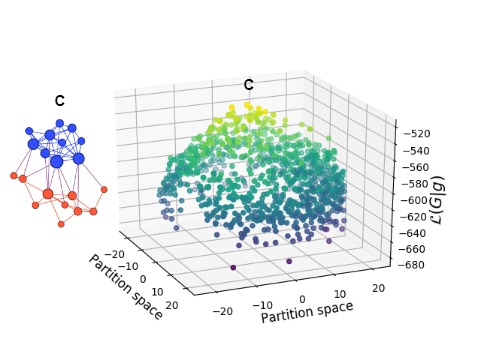
\includegraphics[width=.99\linewidth]{img/chap2/opt_figure_gsbm.jpg}
\caption{Local optima of log-likelihood}
\end{subfigure}
\begin{subfigure}{.45\textwidth} 
\centering
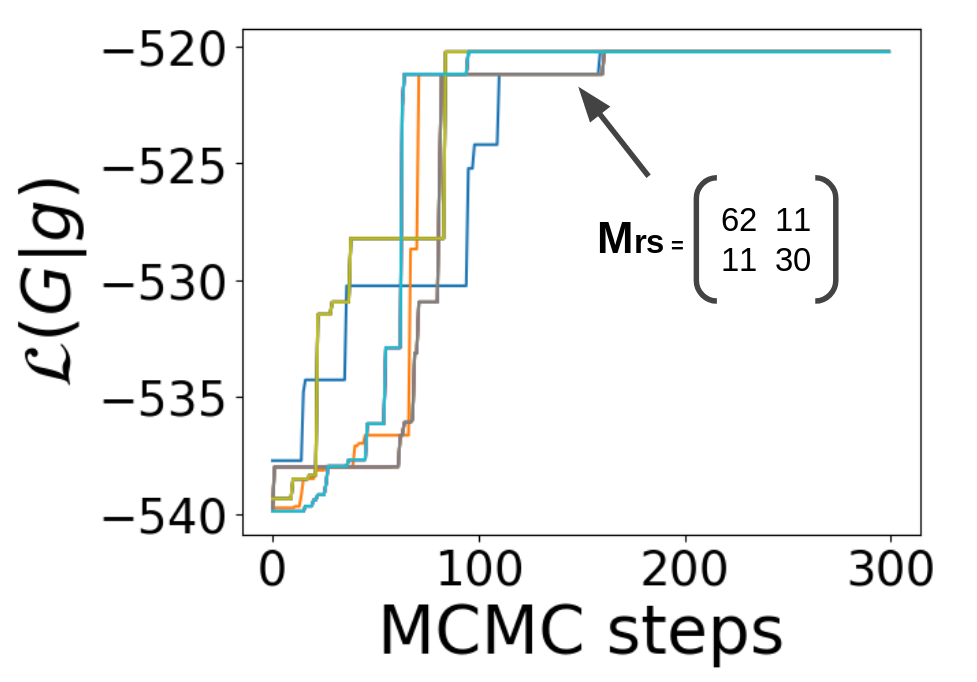
\includegraphics[width=.99\linewidth]{img/chap2/gsbm_converge3.png}
\caption{Convergence}
\end{subfigure}
\caption{The convergence of 20 Markov Chain Monte Carlo (MCMC) trials for the regularized stochastic block model (RSBM) introduced here. All trials converge to the local optimum C which represents an assortative structure. \textbf{(a)} One local optimal partition observed during the MCMC inference for our model. \textbf{(b)} All twenty MCMC trials find the sought-after assortative structure.}
\label{fig:gsbm_3dscatter}
\end{figure*}

We use the networks including Karate club network of Zachary~\cite{zachary1977information}, the Dolphin social network of Lusseau et al.~\cite{lusseau2003bottlenose} and the network of fictional characters' interactions in the novel Les Miserables by Victor Hugo~\cite{newman2004finding} to demonstrate the performance of the regularized model introduced here. The details of each network are presented in the Supplementary Materials. For Karate club network, we evaluate the effect of the regularization terms on the resulting partitions using Markov chain Monte Carlo (MCMC) as the inference algorithm. For every node $i$ in the network, we set the parameter $\theta_i = k_i$ and $f_i = max(f, 1/k_i)$ for our regularized stochastic block model defined by Eq.~\ref{eq:important2} where $k_i$ is the degree of node $i$ and $f_i$ represents the prior in-degree ratio for regularization. Figure~\ref{fig:karate_figure} shows the most likely partition of the Karate club network found by MCMC using different $f$ values. The color represents the block assignment, and the black dashed line divides the network into two parts in the ground truth partition. As shown in Figure~\ref{fig:karate_figure}, when $f=0.14$, the inference algorithm outputs a core-periphery structure which clusters high-degree nodes into the blue block and the remaining low-degree nodes into the red block. This is because the sum of cross entropy terms serves as a regularization term which penalizes those partitions that assign adjacent nodes into the same block. As the value of $f$ grows, the inference algorithm is more likely to detect assortative structure. When $f=0.85$, the inferred block assignment matches the ground truth partition of the Karate club network with the exception of one single red node. However, this node has only one connection to each block; thus, it is quite arguable to which block this node should belong.

\begin{figure*}[!htb]
    \centering
\begin{subfigure}{.3\textwidth} 
\centering
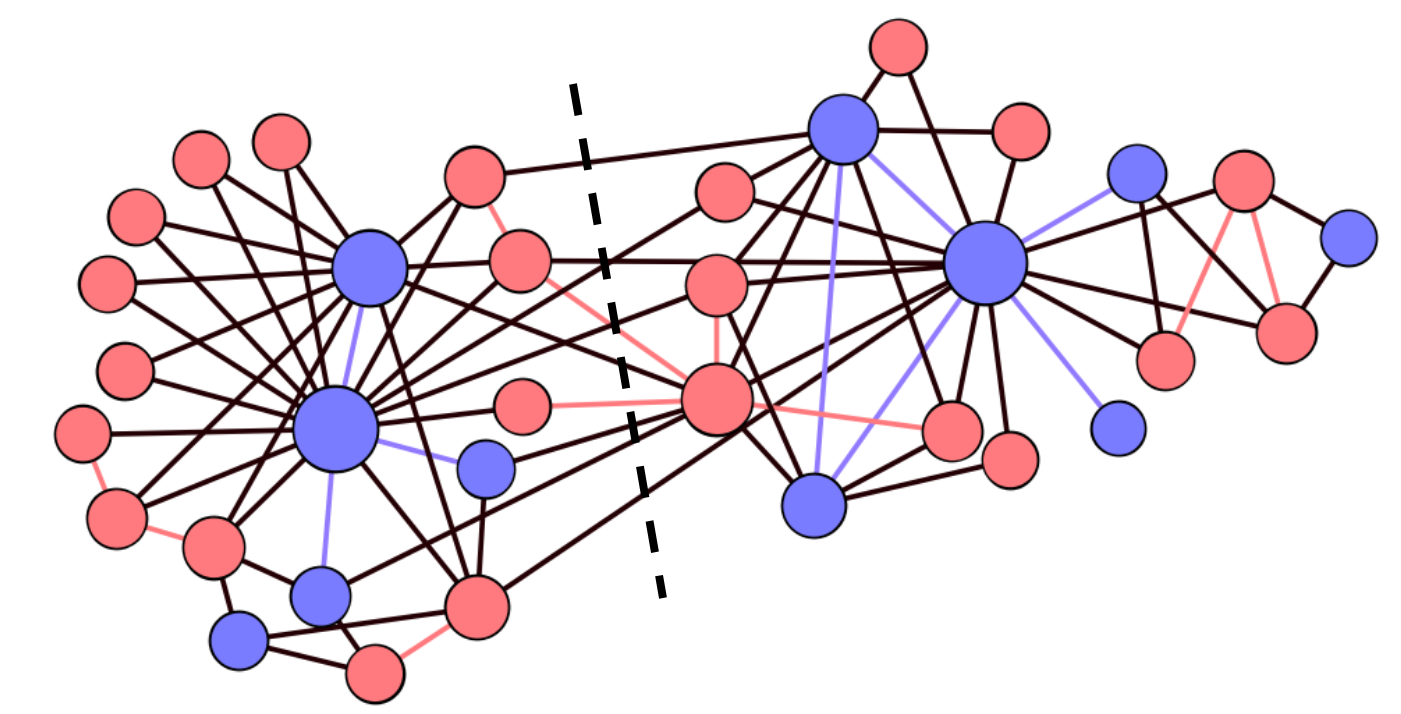
\includegraphics[width=.99\linewidth]{img/chap2/s014.PNG}
\caption{$f=0.14$}
\end{subfigure}
\begin{subfigure}{.3\textwidth} 
\centering
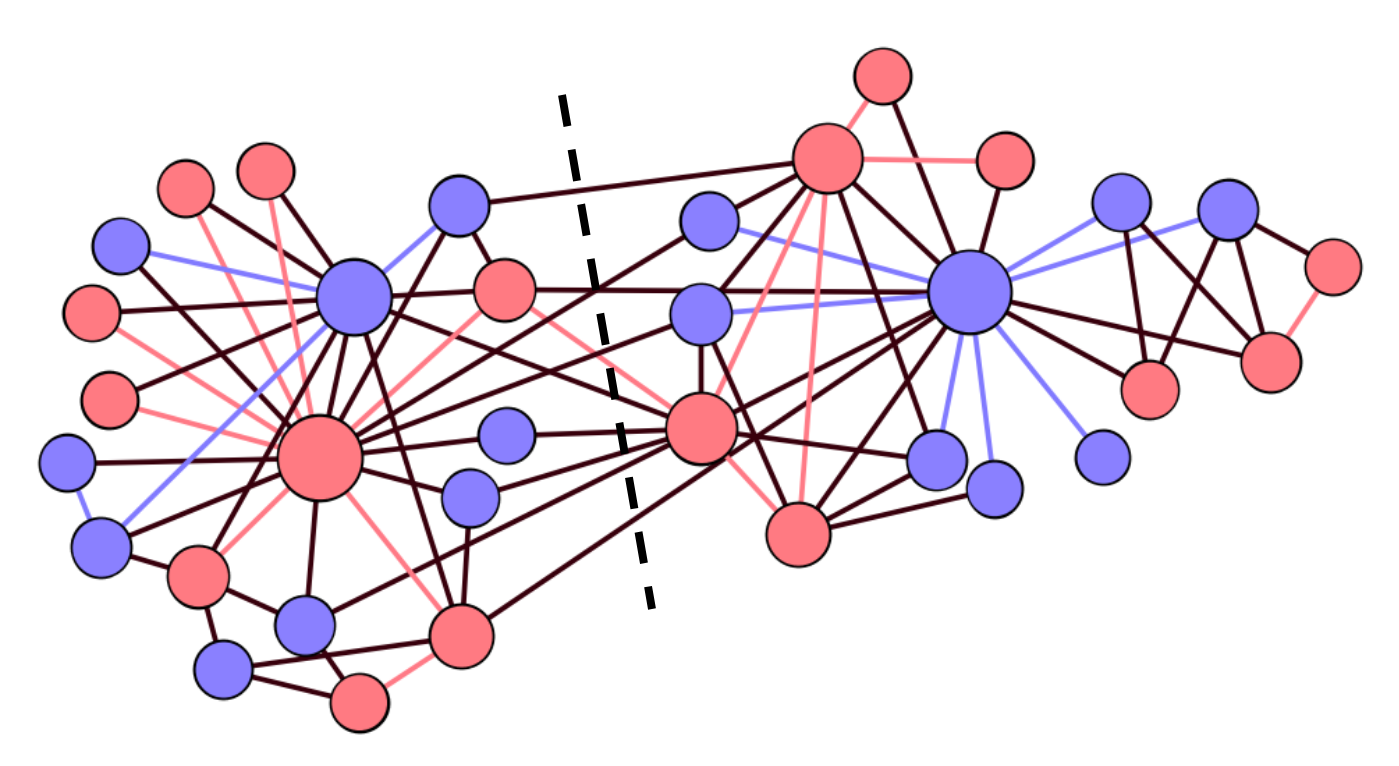
\includegraphics[width=.99\linewidth]{img/chap2/s035.PNG}
\caption{$f=0.35$}
\end{subfigure}
\begin{subfigure}{.3\textwidth} 
\centering
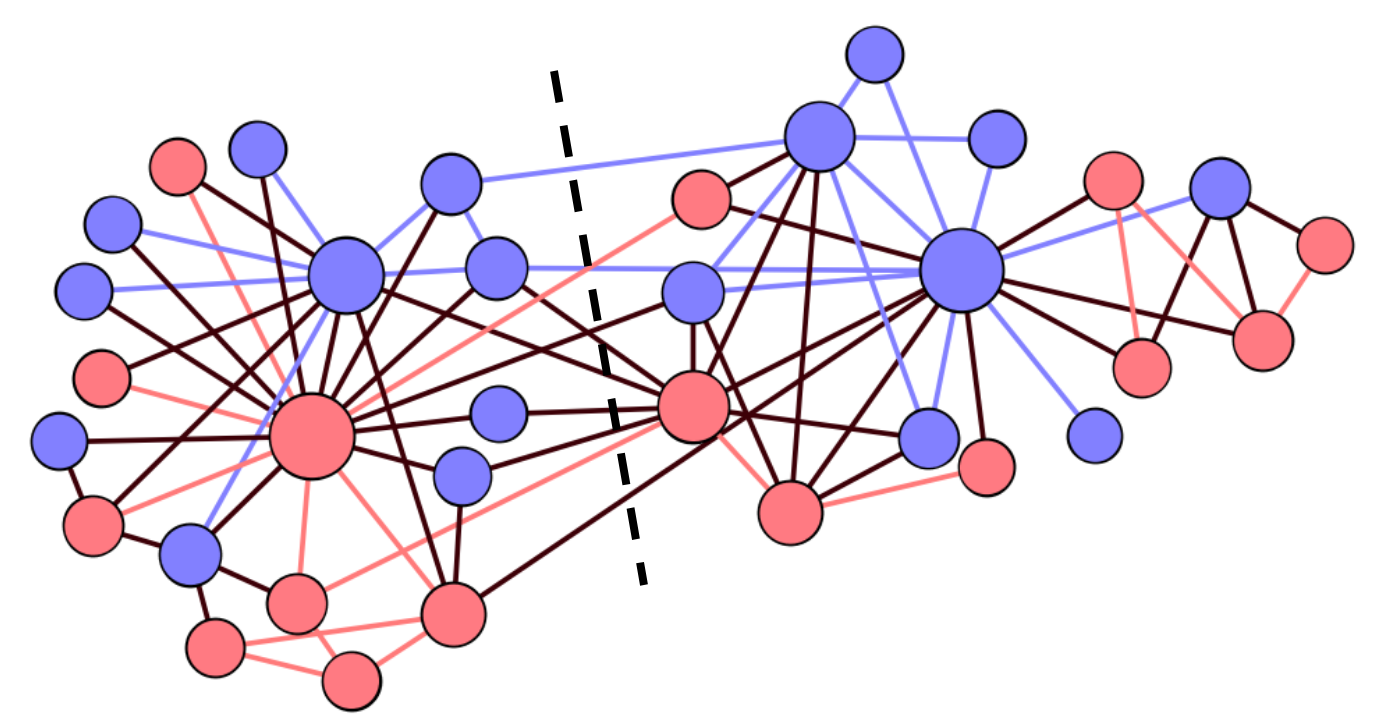
\includegraphics[width=.99\linewidth]{img/chap2/s056.PNG}
\caption{$f=0.56$}
\end{subfigure} %
\hfill

\begin{subfigure}{.3\textwidth} 
\centering
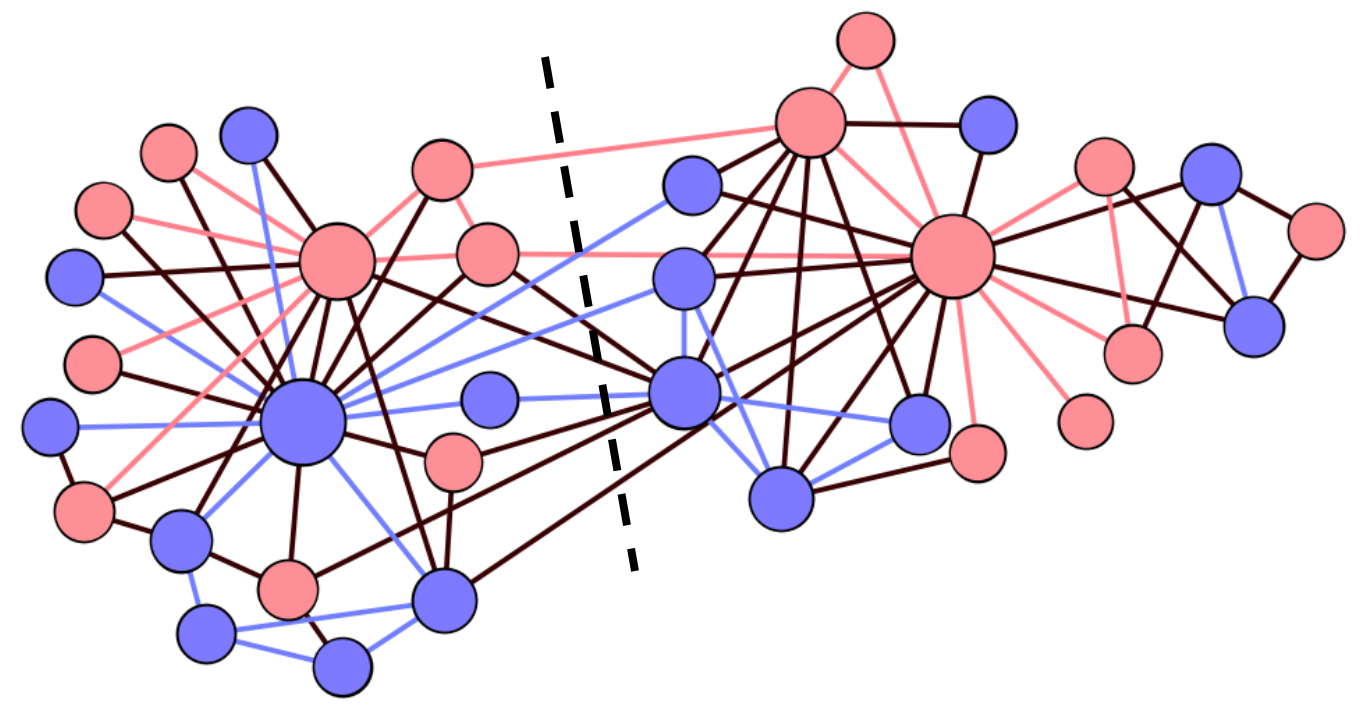
\includegraphics[width=.99\linewidth]{img/chap2/s068.PNG}
\caption{$f=0.68$}
\end{subfigure}
\begin{subfigure}{.3\textwidth} 
\centering
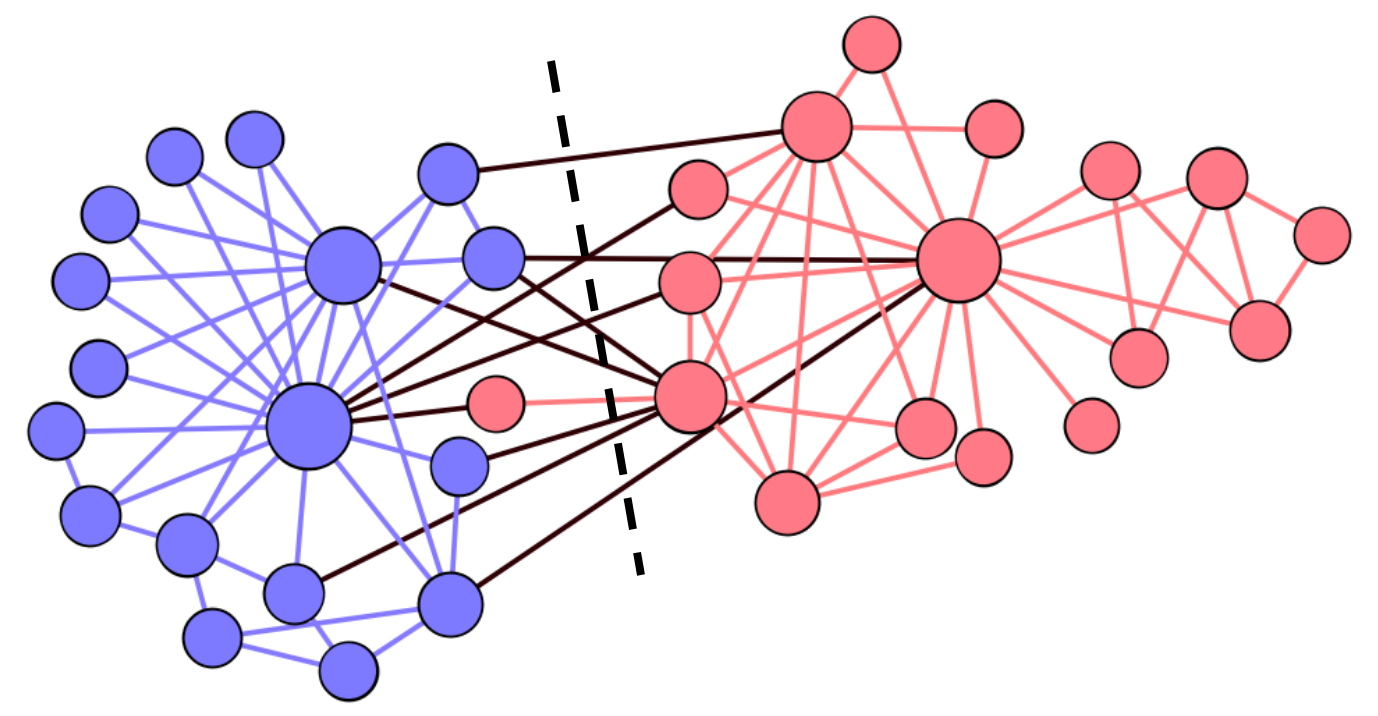
\includegraphics[width=.99\linewidth]{img/chap2/s081.PNG}
\caption{$f=0.81$}
\end{subfigure}

\caption{The partition of Karate network inferred by Markov Chain Monte Carlo under different parameter settings where nodes of the same color belong to the same partition. The black dotted line represents the ideal partition in the ground truth. A small $f$ results in the core-periphery partition of the network while a large $f$ leads to assortative partitions. The values of the $f$ parameter are shown in the corresponding sub-figures captions.}
\label{fig:karate_figure}
\end{figure*}

\begin{figure}[!htb]
    \centering
    
\begin{subfigure}{.3\textwidth} 
\centering
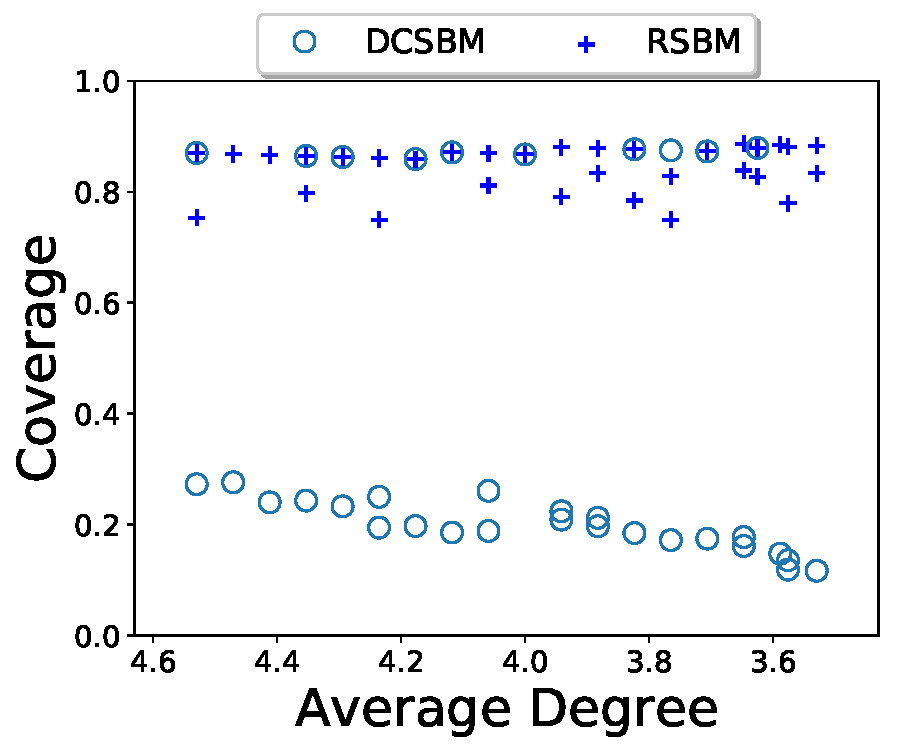
\includegraphics[width=.99\linewidth]{img/chap2/karate_scatter_real.pdf}
\caption{Karate club}
\end{subfigure}
\begin{subfigure}{.3\textwidth} 
\centering
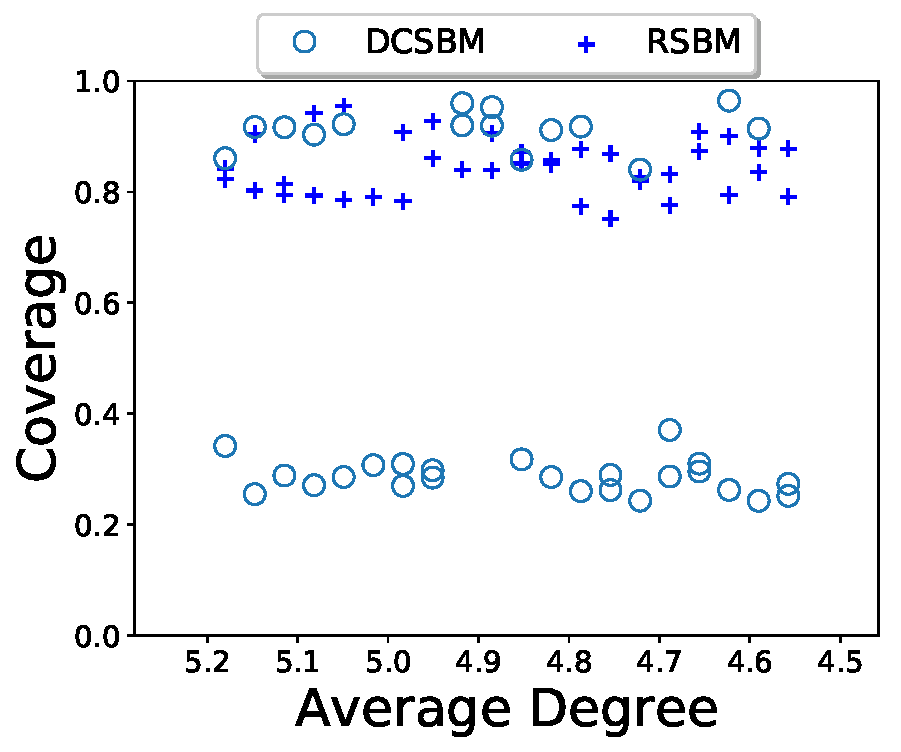
\includegraphics[width=.99\linewidth]{img/chap2/dolphins_scatter_real.pdf}
\caption{Dolphin social}
\end{subfigure}
\begin{subfigure}{.3\textwidth} 
\centering
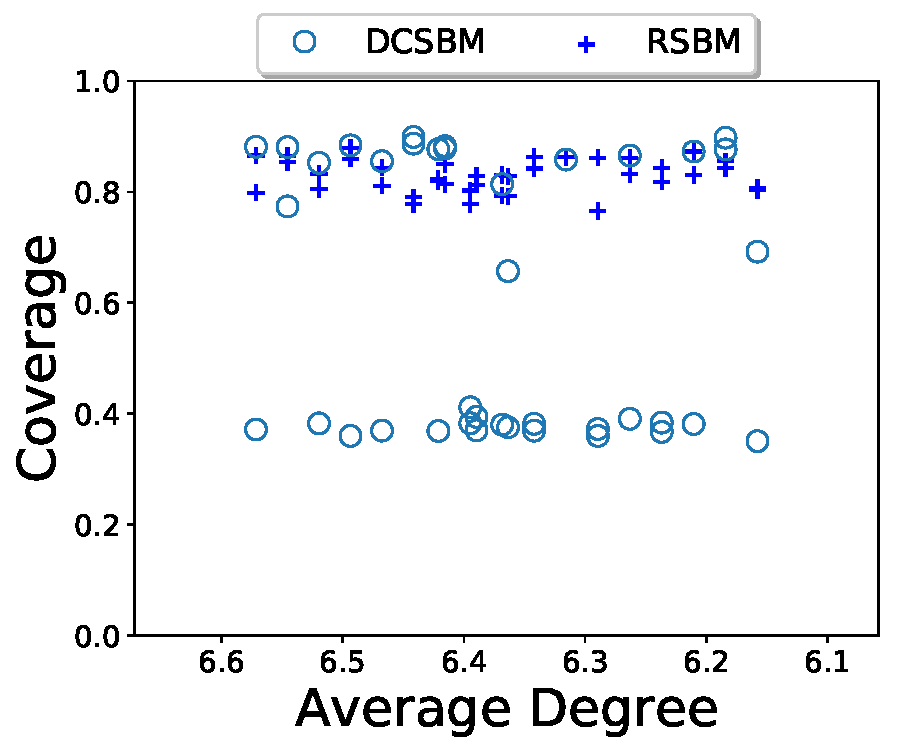
\includegraphics[width=.99\linewidth]{img/chap2/lesmis_scatter_real.pdf}
\caption{Les Miserables}
\end{subfigure}
    
    
    \caption{The \textit{coverage} of partitions in real networks as a function of average node degree. The optimal partitions are inferred by the Markov Chain Monte Carlo algorithm under degree-corrected stochastic block model (DCSBM), marked by circles, and its regularized extension (RSBM) introduce here, marked by crosses. \textbf{(a)} Karate club network~\cite{zachary1977information}; \textbf{(b)} Dolphin social network~\cite{lusseau2003bottlenose}; \textbf{(c)} Characters interaction network of Les Miserables~\cite{newman2004finding}}
    \label{fig:gsbm_real}
\end{figure}

The results in Figure~\ref{fig:gsbm_real} show that the MCMC inference of our RSBM model on these networks finds partitions with higher \textit{coverage} than the ones inferred by the degree-corrected stochastic block model. The \textit{coverage} of a partition~\cite{fortunato2010community} is defined as the ratio of the number of edges with both endpoints in the same block to the total number of edges in the entire network
\begin{equation}
    \text{coverage({\bf g})} = \frac{|\{(i,j)\in E| g_i = g_j\}|}{|E|}
\end{equation}
where $E$ is the set of edges in the network. A low \textit{coverage} indicates that the resulting partition is disassortative. An ideal assortative partition of the network, where all clusters are disconnected, yields a \textit{coverage} of 1.

Figure~\ref{fig:gsbm_real} shows the \textit{coverages} of the partitions found in the three real networks mentioned above. We randomly remove edges in these networks to further increase the sparsity of these networks. And the numbers of blocks used in trials are set to their values for these real networks well-accepted in the literature. The results in Figure~\ref{fig:gsbm_real} indicate that, under degree-corrected stochastic block model (DCSBM), the inference algorithm is likely to miss the assortative structures and returns instead the disassortative partitions of the network, which also fit the model in such cases. In contrast, the MCMC inference of our regularized stochastic block model (RSBM) almost deterministically produces the assortative structures. Interestingly, the inference of degree-corrected stochastic block model produces the partitions with the \textit{coverage} values distributed at two levels. There is no partition with a \textit{coverage} between these two levels found by the inference algorithm. This is similar to the case of the synthetic network in Figure~\ref{fig:dcsbm_3dscatter} where both the assortative communities and disassortative structures fit the degree-corrected stochastic block model. Which structure is found is determined by random sampling of the potential partitions. In other words, there is no way to guide whether the disassortative structures or the assortative communities are preferred, so, two consecutive MCMC trials may return completely different structures.

In contrast, the inference of the introduced here regularized stochastic block model using the prior in-degree ratio $f_i = 0.8 + 0.2 / k_i$ is very robust. It only produces partitions with a high \textit{coverage}, which are generally distributed at the same level as the assortative partitions under degree-corrected stochastic block model. Moreover, the sparsity of the networks does not have an obvious impact on the resulting partitions under our regularized model.

\begin{figure*}[!htb]
    \centering

\begin{subfigure}{.3\textwidth} 
\centering
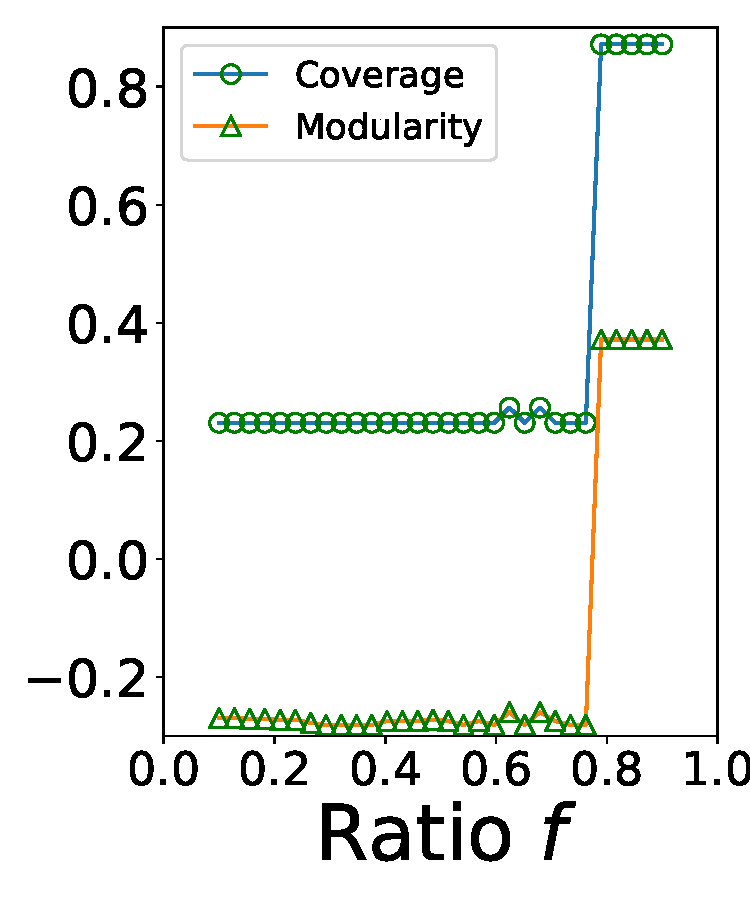
\includegraphics[width=.99\linewidth]{img/chap2/karate_coverage_modularity.pdf}
\caption{Karate club}
\end{subfigure}
\begin{subfigure}{.3\textwidth} 
\centering
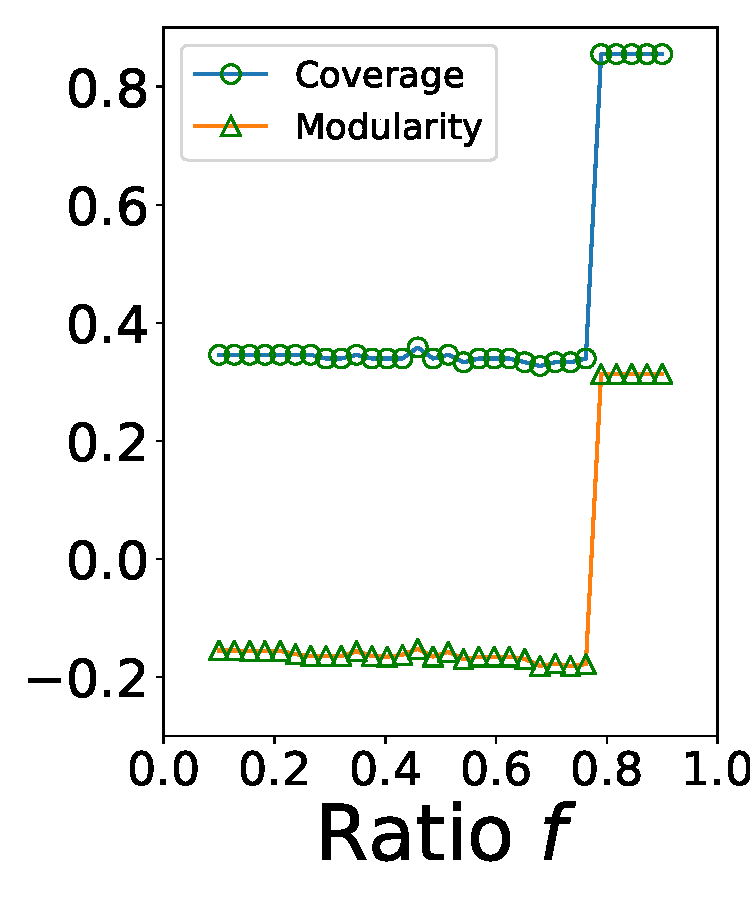
\includegraphics[width=.99\linewidth]{img/chap2/dolphins_coverage_modularity.pdf}
\caption{Dolphin social}
\end{subfigure}
\begin{subfigure}{.3\textwidth} 
\centering
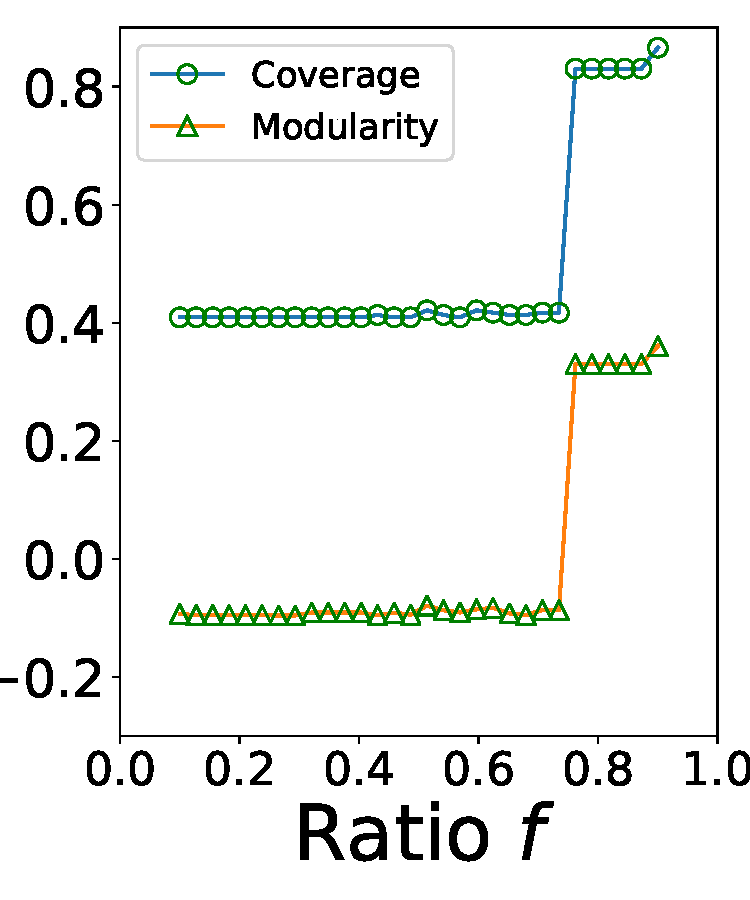
\includegraphics[width=.99\linewidth]{img/chap2/lesmis_coverage_modularity.pdf}
\caption{Les Miserables}
\end{subfigure}

    \caption{The \textit{coverage} and modularity  of partitions in real networks as a function of parameter $f$. The optimal partitions are inferred by Markov Chain Monte Carlo algorithm under degree-corrected stochastic block model (DCSBM) and its regularized extension (RSBM) introduced here. The networks used for evaluation include \textbf{(a)} Karate club network~\cite{zachary1977information}; \textbf{(b)} Dolphin social network~\cite{lusseau2003bottlenose}; \textbf{(c)} Characters interaction network of Les Miserables~\cite{newman2004finding}}.
    \label{fig:gsbm_real2}
\end{figure*}

We evaluate the modularity~\cite{newman2006modularity} of resulting partitions of the real networks as a function of parameter $f$. 
%The modularity  of Newman and Girvan~\cite{newman2006modularity} is a widely used measure to evaluate the quality of network partitions. 
A high modularity indicates the strong community structure. In our experiments, we use a constant $f$ such that $f_i=f$ for each
node $i$ in the network with degree $k_i>1/f$, otherwise $f_i=1/k_i$. We start with a small $f$ value and increase it in each iteration.
The MCMC inference uses as a starting point the original network initially, and the network partition found in the previous iteration subsequently. Figure~\ref{fig:gsbm_real2} shows that, as the value of $f$ increases, in general both the modularity and the \textit{coverage} grow. When $f$ is close to 0, the value of $f$ does not have any effect on the network partition. However, as $f$ becomes larger, then at a certain threshold of about 0.75, the increase of $f$ leads to a critical transition from disassortative partitions to assortative communities. Then, a larger $f$ value does not further increase the modularity  of the partition. These results indicate that, with one single parameter $f$, the Markov Chain Monte Carlo inference gains the flexibility to choose between assortative communities resulting from clustering dense modules of nodes together or disassortative structure, such as the core-periphery structure from clustering high-degree and low-degree nodes into separate blocks. With a choice of high $f$, the inference algorithm is likely to detect assortative communities.


\section{Edge weighting scheme} \label{sec:2.6}
The modularity can be naturally extended to the networks with weighted edges by replacing the count of edges with the sum of their weights. Hence, the weighted modularity is defined as
\begin{equation} \label{eq:definition_weight}
    Q^{w}(G^w, C) = \sum_{c_i \in C} \left[ \frac{W_{c_i}^{in} }{ W } - \left( \frac{W_{c_i}}{ 2 W}\right)^2 \right]
\end{equation}
where $W$ is the sum of weights of edges in the entire graph, $W_{c_i}^{in}$ is the sum of weights of edges within community $c_i$, and the weight of a community is defined as $W_{c_i} = 2W_{c_i}^{in} + W_{c_i}^{out}$ where $W_{c_i}^{out}$ is the sum of weights of edges with exactly one endpoint inside $c_i$. The original definition of modularity is a special case of the weighted version when the weight of every edge is 1.
Many algorithms including~\cite{blondel2008fast,clauset2004finding,newman2004fast,newman2013spectral,sales2007extracting,white2005spectral} were proposed to discover communities in a network by maximizing the modularity. One interesting finding is that Newman's modularity measure is related to the broader family of spectral clustering methods ~\cite{white2005spectral}. There are two categories of spectral algorithms for maximizing modularity: one is based on the modularity matrix~\cite{newman2006finding,newman2006modularity,richardson2009spectral}, the other is based on the Laplacian matrix of a network~\cite{white2005spectral,ruan2008identifying}. The first greedy algorithm, Fast Greedy~\cite{clauset2004finding}, iteratively merges communities in the network to maximize the modularity. Initially, every node is a single community. In every step, two communities joining of which results in the largest modularity among all partitions created by temporary merging one pair of communities are merged together. After $|V|-1$ steps, there is a single community remaining in the network and there are a total of
$|V|$ partitions, each generated by a single step. Then the algorithm outputs the partition with the largest modularity. 
The greedy algorithms solve the maximization problem efficiently, yet they suffer from the resolution limit problem. This problem is defined as an increase of modularity when small well-formed (or ground truth) communities are undesirably joined together into a large community. As pointed out in \cite{fortunato2007resolution,fortunato2016community}, this problem arises because the definition of modularity does not penalize for the increase of the diameter in a community created by merging together smaller ones. In recent work \cite{chen2015new}, Chen et al. introduced a new quality metric, called {\it modularity density}, to limit such bias towards large communities. The new metric is also shown to be able to handle another known weakness of modularity, the counterproductive splitting of large communities. This is because the modularity density takes into account the density of discovered communities and penalizes the splitting of large communities. The fine-tuned $Q_{ds}$ algorithm \cite{chen2014community} was proposed to maximize this new quality metric.

%%%%%%%%%%
%%%%%%%%%%
%%%%%%%%%%

\subsection{Properties of balanced edge weighting scheme}

Instead of proposing a new community detection algorithm, we invent an efficient edge weighting scheme to improve the performance of the current state-of-art algorithms. As shown in~\cite{fortunato2007resolution}, for the modularity maximization to be able to find a community $c_i$ with $|E^{in}_i|$ edges inside, the following inequality must hold,
\begin{equation}
|E^{in}_i| \geq \sqrt{\frac{|E|}{2}}.
\end{equation}
where $E^{in}_i$ is the set of the edges inside community $c_i$, and $E$ is the set of edges of the entire graph. In large networks with millions of edges, the number of edges in most communities is often smaller than this lower bound. In~\cite{berry2011tolerating}, it has been shown that edge weighting scheme is capable of decreasing such theoretical bound and enhancing community detection performance in practice. Inspired by this result, we define the edge weighting scheme that \textit{enhances} particular community as follows.
\begin{rmk} An edge weighting scheme \textit{enhances} a community $c_i$ by sum of additional weights $e_i=\sum_{e\in {E^{in}_{c_i}}} (w_e - 1)>0$ if $w_e \geq 1$ for $\forall e \in E^{in}_{c_i}$,  and $w_e \leq 1 $ for $\forall e \in E^{out}_{c_i}$ while $W_{c_i} = d_{c_i}$ holds. Such a scheme is a {\it balance enhancement} if both communities connected by the cross-community edge with decreased weight are enhanced. \end{rmk}
The edge weighting scheme \textit{enhances} a community $c_i$ by increasing the weights of edges residing within this community with added total weight of $e_i>0$ , while reducing the weight of edges crossing to other communities by $2e_i$ to preserve the weight of the community $W_{c_i}$ equal to $d_{c_i}$. It is worth noting that a balanced enhancement preserves the total weight of the original graph, which is $W = |E|$. Here, we show that such balanced weighting scheme is non-decreasing modularity operation on a graph.
\begin{thm}  \label{theorem:1} $Q^w(G^w, C) \geq Q(G, C)$ if the weighting scheme is balanced. \end{thm}
\noindent \textbf{Proof:} 
For any community $c_i$, 
\begin{equation}
W^{in}_{c_i} = \sum_{e\in E^{in}_{c_i} } w_e \geq \sum_{e\in E^{in}_{c_i} } 1 = |E_{c_i}^{in}|.
\end{equation}
Thus,
\begin{align}
    Q^{w}(G^w, C) & = \sum_{c_i \in C} \left[ \frac{W_{c_i}^{in} }{ W } - \left( \frac{W_{c_i}}{ 2 W}\right)^2 \right]\\
    & \geq \sum_{c_i \in C} \left[ \frac{|E_{c_i}^{in}| }{ |E| } - \left( \frac{d_{c_i}}{ 2 |E|}\right)^2 \right]\\
    & = Q(G, C).
\end{align}
Although the edge weighting scheme which \textit{enhances} one community in a partition always increases this community's modularity, it does not necessarily guarantee that such enhanced partition would maximize modularity in the weighted graph. Here, we define a notion of locally maximal partition and prove that the proper edge weighting scheme can preserve such property.
\begin{rmk} Modularity of a partition $C$ is \textit{locally maximal} if the modularity decreases upon splitting any community in $C$ or joining any two communities in $C$. \end{rmk}
\begin{thm} \label{theorem:2} $\Delta Q^w_{c_i,c_j}\leq \Delta Q_{c_i,c_j}$ if $c_i,c_j$ are enhanced by the balanced edge weighting scheme.\end{thm}
\noindent \textbf{Proof:} 
Without loss of generality, consider two ground truth communities $c_i$ and $c_j$ \textit{enhanced} by the balanced edge weighting scheme. The change in modularity $Q^w$ upon joining these two communities is,
\begin{align} \label{eq:change}
\Delta Q^w_{c_i,c_j} &=  \frac{W_{c_i, c_j}}{W} - \frac{W_{c_i}W_{c_j}}{2W^2} = \frac{W_{c_i, c_j}}{|E|} - \frac{d_{c_i} d_{c_j}}{2|E|^2}\\
& \leq \frac{|E_{c_i, c_j}|}{|E|} - \frac{d_{c_i} d_{c_j}}{2|E|^2} = \Delta Q_{c_i,c_j}
\end{align}
\begin{thm} \label{theorem:3} If community $c$ with $d_{c} \leq \sqrt{8|E|}$, is enhanced by the balanced edge weighting scheme and split into communities $c_i,c_j$ and $\Delta Q_{c_i,c_j}\geq 0$ then also $\Delta Q^w_{c_i,c_j}\geq 0$.
\end{thm}
\noindent \textbf{Proof:} 
Consider a community $c=c_i\cup c_j$ with $d_c \leq \sqrt{8|E|}$ \textit{enhanced} by the balanced edge weighting scheme, where $c_i$ and $c_j$ are two non-empty communities, then $\Delta Q_{c_i,c_j} \geq 0 $ by assumption that modularity reaches local maximum for partition $C^*$.
If $E_{c_i,c_j} = \emptyset$, then $W_{c_i, c_j} = 0$ and $ \Delta Q_{c_i,c_j} = - \frac{d_{c_i} d_{c_j}}{2|E|^2} \geq 0$. This leads to either $d_{c_i}=0$ or $d_{c_j}=0$ which causes contradiction. Otherwise, if $|E_{c_i,c_j}| \geq 1$, then $W_{c_i, c_j} \geq 1$ because the edge weighting scheme assigns weight $w_e \geq 1$ to any edge $e \in E_{c_i,c_j}$. Since $W_{c_i} + W_{c_j} = W_c = d_c$, we have $W_{c_i}W_{c_j} \leq (\frac{d_c}{2})^2$. When community $c$ splits into communities $c_i$ and $c_j$, the change in modularity $Q^w$ is,
\begin{align}
- \Delta Q^w_{c_i,c_j} &=  \frac{W_{c_i}W_{c_j}}{2W^2} - \frac{W_{c_i, c_j}}{W}\leq \frac{(\frac{d_c}{2})^2}{2W^2} - \frac{1}{W}\\
&= \frac{(d_c)^2 - 8 W }{8W^2} = \frac{d_c^2 - 8 |E| }{8|E|^2}\leq 0
\end{align}
Note that the last inequality holds because of the condition $d_c\leq \sqrt{8|E|}$.
From Theorems~\ref{theorem:2} and~\ref{theorem:3} it follows immediately that if partition $C^*$ is locally maximal and each community $c$ satisfies
the condition $d_c \leq \sqrt{8|E|}$ and is enhanced by the balanced edge weighting scheme, the modularity of this partition is locally maximal also for the weighted graph $G^w$.
Since, by Theorem~\ref{theorem:2}, joining communities $c_i$ and $c_j$ makes change $\Delta Q^w_{c_i,c_j}\leq \Delta Q_{c_i,c_j}$, it is entirely possible that $\Delta Q^w_{c_i,c_j}\leq 0 <\Delta Q_{c_i,c_j}$. Thus, modularity maximization for the graph with the enhanced weights will avoid joining possibly well-formed communities $c_i$ and $c_j$ while the maximization on the original graph would join them. This example demonstrates that if the well-formed small communities are \textit{enhanced}, then their chances of being detected will increase. This observation motivates us to propose a regression model for assigning weights to edges so that the real ground truth communities can be \textit{enhanced} in a network.
\subsection{Graph sampling and edge weights regression}
We follow the same paradigm of the original modularity maximization to detect communities but seek to assign weights to the edges to improve the quality of results. To be precise, a regression model is developed to convert an unweighted graph $G$ to a weighted graph $G^{w}$ so that modularity maximization finds communities of better quality by maximizing modularity in $G^{w}$ rather than in $G$. The regression model takes the local topological features of edges as input and outputs the weight of every edge. As illustrated in Figure~\ref{fig:illustration}, the proposed procedure is divided into the following three steps:
\begin{itemize}
    \item {\bf Artificial network construction} done to estimate the network parameters of the input graph and construct a similar artificial graph in which the ground truth communities are known beforehand by construction. The goal is to ensure these ground truth communities can be successfully separated in the modularity maximization process.
    \item {\bf Edge feature extraction} executed on the edges of the artificial graph. The edge features are used as input to the regression model.
    \item {\bf Regression on edge weights} uses a regression model to compute the edge weights such that the modularity maximization is able to separate adjacent ground truth communities in the artificial network.
\end{itemize}
\begin{figure}
    \centering    
    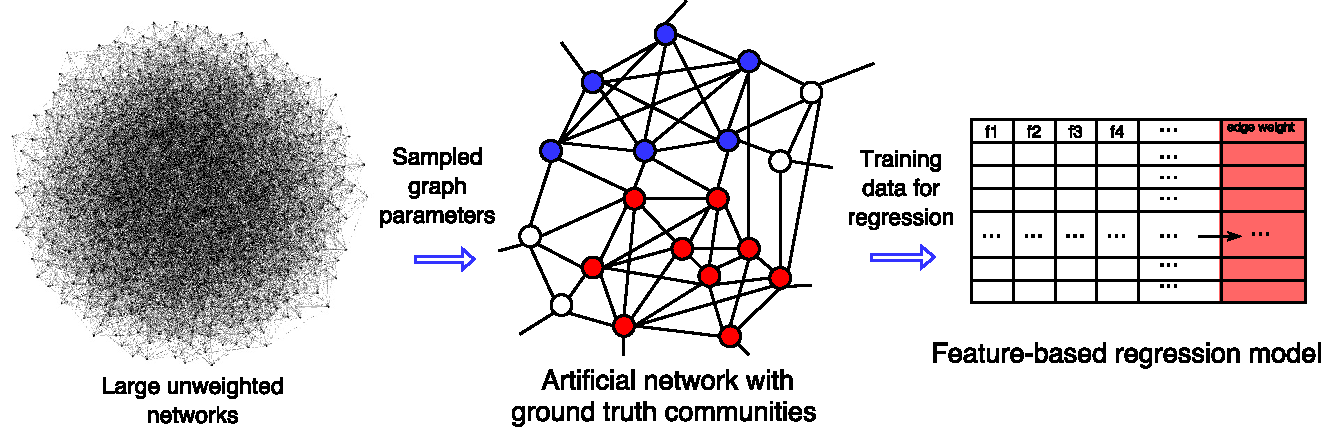
\includegraphics[width=\textwidth]{img/chap2/illustration2.pdf}
    \caption{Illustration of the adaptive modularity maximization.}
    \label{fig:illustration}
\end{figure}
Given a large unweighted input graph, our approach constructs an artificial network which shares degree distribution and clustering coefficients with the input graph. Specifically, multiple Stochastic Block Model (SBM) networks~\cite{holland1983stochastic} are created with high intra-block edge densities and with a few randomly chosen inter-block edges, resulting in a relatively small inter-block edge density and with blocks forming ground truth communities. Then, the edges in these SBM graphs are randomly removed from network instances until the average node degree becomes close to that of the input graph. Among all SBM network instances, the one with the average clustering coefficient closest in its value to the input graph is chosen as the final artificial network.
The ground truth communities (i.e., the nodes in blue and red in Figure~\ref{fig:illustration}) in the artificial network are used as training data to infer the parameters of the regression model. As Theorem~\ref{theorem:2} suggests, if the correct communities have been enhanced, then the probability of properly detecting these communities would increase. Therefore, the regression model incorporates these ground truth communities into the detection algorithm framework to enhance it.
Since communities are considered local structures, the second step of our approach is to extract the local topological features of every edge in the network. For each edge $e=(u,v)$ in the graph, the following local topological features are extracted efficiently from the network.
\\
\textbf{f-1}. The square root of the number of common neighbors, $\sqrt{\N(u) \cap \N(v)}$, where $\N(v)$ denotes the set of neighbors of node $v$. 
\\
\textbf{f-2}. The difference in clustering coefficients of the endpoints, $|c(u) - c(v)|$, where $c(v)$ denotes the clustering coefficient of node $v$. 
\\
\textbf{f-3}. Jaccard-coefficient which is defined as
\begin{equation}
\text{Jaccard}(u,v) = \frac{|\N(u) \cap \N(v) |}{|\N(u) \cup \N(v) |}
\end{equation}
\\
\textbf{f-4}. Resource allocation index which is defined as
\begin{equation}
\bigcup_{w \in \N(u) \cap \N(v)} \frac{1}{|\N(w)|}
\end{equation}
\\
\textbf{f-5}. Adamic-Adar index which is defined as
\begin{equation}
\bigcup_{w \in \N(u) \cap \N(v)} \frac{1}{\log|\N(w)|}
\end{equation}
\\
\textbf{f-6}. Relative degree ratio which is defined as
\begin{equation}
\text{rel}(u,v) = \frac{\min(|\N(u)|,|\N(v)|) }{\max(|\N(u)|,|\N(v)|)}
\end{equation}
When the degrees of nodes $u$,$v$ are equal, $\text{rel}(u,v) = 1$.
The attributes of edges or nodes, such as text content and user profiles, can also be used as features, if they are available. Using more local topological features generally leads to better accuracy because more information is embedded in these features.
As pointed out in \cite{fortunato2007resolution}, community detection algorithms based on modularity maximization tend to execute counterproductive merges of small communities into large ones. One way to handle this resolution limit problem is to cause such merging operations to decrease the modularity. 
According to the definition of weighted modularity, the change in $Q$ upon joining two communities $c_i$ and $c_j$ is
\begin{equation} \label{eq:delta_Q}
\Delta Q^w_{c_i, c_j} = \frac{W_{c_i,c_j}}{W} - \frac{W_{c_i} W_{c_j}}{2W^2}
\end{equation}
where $W_{c_i,c_j}$ is the sum of weights of the edges between $c_i$ and $c_j$, $W_{c_i} = 2W_{c_i}^{in}+W_{c_i}^{out}$ is twice the sum of weights of the edges inside community $c_i$ plus the sum of weights of the edges with exactly one edge in $c_i$, and W is the sum of weights of all edges.
To avoid the merging of some pairs of small communities $\{(c_i^1, c_i^2)\}_{i\in I}$ existing in the artificial networks
described in Section 4.2, joining them should cause a decrease of modularity, hence
\begin{equation} \label{eq:avoid}
     \Delta Q^w_{c_i^1, c_i^2} \leq 0 \hspace{2em} \text{for $i \in I$}
\end{equation}
where $I$ is the parameter defining number of pairs of small communities to be selected from the artificial network.
Using the penalty method, the optimization problem can be formulated as
\begin{align} \label{eq:opt_w}
\min_{w}  \hspace{1em} F(w) = ( \bar w - 1)^2 + \lambda_1 \sigma_w^2 + \lambda_2 \sum_{ 1 \leq i \leq I} h( \Delta Q_{c_i^1, c_i^2} )
\end{align}
where $w = \{w_e\}$ is the set of the weights of edges in the entire graph, $\sigma_w^2$ is the variance of the edge weights, $\bar w$ is the average edge weight $\frac{\sum_{e \in E} {w_e}}{|E|}$, $h(x)$ is the loss function such as the sigmoid function $h(x) = \frac{1}{1 + e^{-x}}$, $\lambda_1$ is a constant, and $\lambda_2$ is a coefficient for the penalty terms. 
The regularization term $(\bar w - 1)^2 $ ensures that the resulting average edge weight is close to 1. Using regularization on $\bar w$ directly is likely to result in very small weights that are inconvenient in community detection tasks. For the same reason, the regularization on the variance of edge weights $\sigma_w^2$ limits the total number of negative edges. When $\lambda_1 \gg \lambda_2$, the above optimization problem converges at $w_e = 1$ for $\forall e \in E$, yielding the weights of edges in an unweighted graph.
So far, we have presented an optimization method of modifying edge weights which helps avoiding improper merging of communities. However, it involves as many variables as the total number of edges and does not guarantee that edges with similar features have similar weights. Let's denote the $i$-th topological feature of one edge $e$ as $x_e^{<i>}$. The weight of an edge $e$ is obtained by the linear regression
\begin{equation} \label{eq:regression}
w_e = p_0 + \sum_{i=1}^{r} p_i x_{e}^{<i>}
\end{equation}
where $p_i$ is the parameter of the $i$-th feature, for $i=1,\ldots,r$. Let the feature vector of an edge $e$ be $x_e = (1,x_e^{<1>},x_e^{<2>},\ldots,x_e^{<r>})^T$. Then Eq.~\ref{eq:regression} can be rewritten as
\begin{equation} 
w_e = p^T x_{e}
\end{equation}
where vector $p=(p_0,p_1,\ldots,p_r)^T$. This way, the objective function in Eq. \ref{eq:opt_w} becomes a function over $p$.
The first order partial derivative of the objective function over $p_i$ is
\begin{align} \label{eq:foverp}
\frac{ \partial F(w(p))}{\partial p_i} = \frac{ \partial F(w)}{\partial w} \times \frac{ \partial w}{\partial p_i}
\end{align}
The second term on the right side of the above equation is
\begin{align} \label{eq:woverp}
\frac{ \partial w}{\partial p_i} = \left(  x^{<i>}_1,x^{<i>}_2,\ldots,x^{<i>}_{|E|} \right)
\end{align}
The first term on the right side of Eq. \ref{eq:foverp} is
\begin{equation} \label{eq:foverw}
\frac{ \partial F(w)}{\partial w} = \frac{\partial (\bar w - 1)^2 }{\partial w} + \lambda_1 \frac{\partial \sigma_w^2 }{\partial w} + \lambda_2 \sum_{i \in I} \frac{ \partial h(\Delta Q^w_{c_i^1, c_i^2})}{\partial \Delta Q^w_{c_i^1, c_i^2} } \frac{ \partial \Delta Q^w_{c_i^1, c_i^2}}{\partial w} 
\end{equation}
where the partial derivative $\frac{ \partial h(\Delta Q_{c_i^1, c_i^2})}{\partial \Delta Q_{c_i^1, c_i^2} }$ is obtained from the specific loss function $h()$. It is also easy to compute the partial derivative $\frac{ \partial \Delta Q^w_{c_i^1, c_i^2}}{\partial w} $ according to Eq.~\ref{eq:delta_Q}.
\textbf{Algorithm}. To solve the optimization problem presented above, we can apply a quasi-Newton method, such as the Broyden-Fletcher-Goldfarb-Shanno (BFGS) algorithm~\cite{nocedal2006numerical}, which requires only the first derivative of the objective function to find the optimal result. The pseudo code of the training algorithm is presented in Algorithm \ref{algo:1}.
During the training phase, $|I|$ pairs of ground truth communities $\{c_i^1,c_i^2\}_{i \in I}$ can be chosen randomly from the artificial network assuming that the ground truth communities are provided. One efficient way to obtain the required number of pairs of ground truth communities is to sample adjacent communities in the artificial network randomly until $|I|$ pairs are collected. As indicated by Theorem~\ref{theorem:3}, small communities are preferred to large communities here. Hence, we can set an upper bound on the size of the chosen communities. After the parameters are inferred, the regression model which assigns weights to edges can be applied to enhance the performance of community detection algorithms.

\begin{algorithm}[ht!]
\caption{Regression Model Training Algorithm}
\begin{algorithmic}[ht!] \label{algo:1}
\State Initialize p
\For {each edge $e$}
\State $x_e \leftarrow$ extracted features of edge $e$
\State $w_e \leftarrow p^T x_e$
\EndFor
\State $tol \leftarrow 0.0001$
\State Construct $\{c_i^1,c_i^2\}_{i\in I}$
\Repeat
\State Compute $\frac{ \partial F}{\partial w}$ using Eq. \ref{eq:foverw}
\State $ \frac{ \partial F}{\partial p} \leftarrow \frac{ \partial F}{\partial w} \times \frac{ \partial w}{\partial p} $
\State Update $p$ via one BFGS step
\For {each edge $e$}
\State $w_e \leftarrow p^T x_e$
\EndFor
\Until {$\|\frac{ \partial F(w(p))}{\partial p}\| < tol$ or the maximum number of iterations is made}
\end{algorithmic}
\end{algorithm}

The \textbf{time complexity} of Algorithm 1 is $O(k(|I|+|E_a|))$ where $k$ is the number of BFGS iterations before the algorithm converges, $|I|$ is the number of constraints in Eq. \ref{eq:avoid} and $|E_a|$ is the total number of edges in the artificial graph. In order to accelerate the computation, we adopt the following key speedup improvements.
To compute the change of modularity upon joining two communities, the weights of all edges in the artificial graph need to be summed up which takes significant amount of time in each BFGS step. The summation of weights is
\begin{equation} \label{eq:sumofweight}
    W = \sum_{e\in E_a} {w_e} = \sum_{e\in E_a} p^T x_e = p^T \sum_{e\in E_a} {x_e}
\end{equation}
which can be calculated efficiently because $\sum_e {x_e}$ needs to be computed only once at the outset of the optimization process, and $W$ is re-computed as the inner product of $p$  and $\sum_e {x_e}$ in every iteration. The sums of weights of the edges related to each community $c$, such as $W^{in}_c$ and $W^{out}_c$, and the variance of edge weights $\sigma_w^2$ can also be computed in the similar manner. Note that such speedup can be achieved because we intentionally use linear regression to compute the edge weights in Eq. \ref{eq:regression}. Otherwise, if non-linear regression function is used to obtain the edge weights, Eq. \ref{eq:sumofweight} does not hold and it generally takes more time to
obtain the sums of weights.
In our algorithm, the edges with both endpoints not in any communities in pairs $\{c_i^1, c_i^2\}$ for $i\in I$ are not involved in the computation of every BFGS iteration. The number of edges involved in every BFGS iteration is at most $2|I|Z$ where $Z$ is the average number of edges in communities in pairs $\{c_i^1, c_i^2\}$. So, the time complexity is reduced to $O(|E_a| + k|I| \times 2|I|Z) = O(|E_a| + k|I|^2Z)$. In practice, this accelerated algorithm provided at least a 50-fold speedup compared to Algorithm 1. 

The state-of-art greedy modularity maximization algorithm, Fast Greedy~\cite{clauset2004finding}, is executed on several real and synthetic networks. The details of the tested networks are summarized in Table~\ref{table:summary}.  We evaluate the execution time of the training of the regression model and the additional time needed to convert an unweighted graph into a weighted one. We does not report the time cost of community detection, which depends on the specific algorithms. Hence, the reported time cost consists of two parts: (i) Training: the time cost to infer all the parameters of the regression model from the artificial graph; (ii) Weighting: the time cost to compute the weights of every edge in the original graph. Note that both parts include the I/O cost of loading the network files from disk and the edge topological feature extraction time.
\begin{table}[!t]
\caption{Summary of the networks}
\label{table:summary}
\centering
\setlength\tabcolsep{2pt}
\begin{tabular}{ c|c|c|c|c }
 \hline
No. & Network & \#Nodes & \#Edges & Type\\
 \hline
1 & American college football & 115 & 613 & Real \\
2 & LFR benchmark & 5000 & $\approx$35000  & Synthetic\\
3 & Amazon product co-purchasing network & 334863 & 925872 & Real\\
4 & DBLP collaboration network & 317080 & 1049866 & Real \\
 \hline
\end{tabular}
\end{table}

The LFR benchmark networks~\cite{lancichinetti2008benchmark} serve as one of the standards for the evaluation of community detection algorithms. The properties of the network generated from the benchmark are defined by the following three parameters: $\gamma$ which is an exponent of the node degree in the power law distribution, $\beta$ which is an exponent of the community size in the power law distribution, and $\mu$ which is the mixing parameter that defines the fraction of edges originating in a community that have one endpoint outside of it. In our experiments, every LFR benchmark network has 5,000 nodes with the average node degree 15 and the maximum node degree 50. The exponents $\gamma$ and $\beta$ are set as 2 and 1 respectively and the mixing parameter $\mu$ takes two values, 0.45 and 0.5, which are quite challenging because high values of the mixing parameter are likely to result in loose community structures. Considering the randomness in the generation of synthetic networks, 10 network instances are constructed for each $\mu$ value.

We evaluate the modularity maximization performance on the original unweighted LFR benchmark networks. Table~\ref{table:LFR} lists the results of the following algorithms Fast Greedy modularity maximization algorithm (FG) on the original unweighted graphs and Fast Greedy modularity maximization algorithm (FG-w) running on the weighted graphs produced by our model. As seen in Table~\ref{table:LFR}, the performance of the Fast Greedy (FG) algorithm~\cite{clauset2004finding} has been significantly improved by maximizing the modularity on the weighted networks instead of on the original unweighted graph. The F-measure is improved by nearly 40\% and the NMI metric is improved by 25\% in all cases. In Table~\ref{table:LFR}, the modularity $Q$ and modularity density $Q_{ds}$ values are all computed over the original unweighted LFR benchmark networks. This surprising result shows that the execution of Fast Greedy algorithm on weighted graph can improves the $Q_{ds}$ value for the corresponding unweighted graph. In other words, the weighted edges allows the greedy algorithm to escape from local maximum of $Q_{ds}$ and get better value of it on the original unweighted graph. Also, using the edge weighting scheme, the Fast Greedy algorithm which maximizes the weighted modularity performs better than the fine-tuned $Q_{ds}$ algorithm~\cite{chen2014community}. In addition, we compared our approach to the previously published algorithm CNM~\cite{berry2011tolerating}. The introduced here edge weighting scheme achieves an average 85\% Jaccard-index score while the CNM algorithm obtains the average score of 82\% on 10 different realizations of the LFR benchmark networks using the same parameters, with the mixing parameter set to $\mu=0.5$. The remaining specific construction parameters of these LFR benchmark networks and the definition of Jaccard-index can be found in~\cite{berry2011tolerating}.
\begin{table}[!t]
%\renewcommand{\arraystretch}{1.3}
\caption{Metric values characterizing the community structures computed over the original unweighted LFR benchmark networks but discovered by different algorithms.}
\label{table:LFR}
\centering
\setlength\tabcolsep{2pt}
\begin{tabular}{|c|c||c|c|c|c|c|c|}
\hline
$\mu$ & Method & VI & NMI & F-measure & ARI & $Q$ & $Q_{ds}$ \\
\hline
\hline
\multirow{3}{*}{0.45} & FG &3.2135&0.5953&0.3379&0.2355&0.4214&0.0366\\
\hhline{~-------}
& Fine-Tuned $Q_{ds}$ & 1.1523 & 0.8925 & 0.8806 & 0.7337 & 0.4536 & 0.1632\\
\hhline{~-------}
& FG-w & 0.0137 & 0.9987 & 0.9990 & 0.9972 & 0.5152 & 0.1668\\
\hline
\multirow{3}{*}{0.5} & FG &3.5187&0.5481&0.2937&0.1993&0.3739&0.0274\\
\hhline{~-------}
& Fine-Tuned $Q_{ds}$ & 1.9677 & 0.8036 & 0.7489 & 0.4984 & 0.3563 & 0.1196\\
\hhline{~-------}
& FG-w & 0.0678 & 0.9934 & 0.9950 & 0.9864 & 0.4625 & 0.1381\\
\hline
\end{tabular}
\end{table}
\begin{figure}[!ht]
\centering
\begin{subfigure}{.3\textwidth} 
\centering
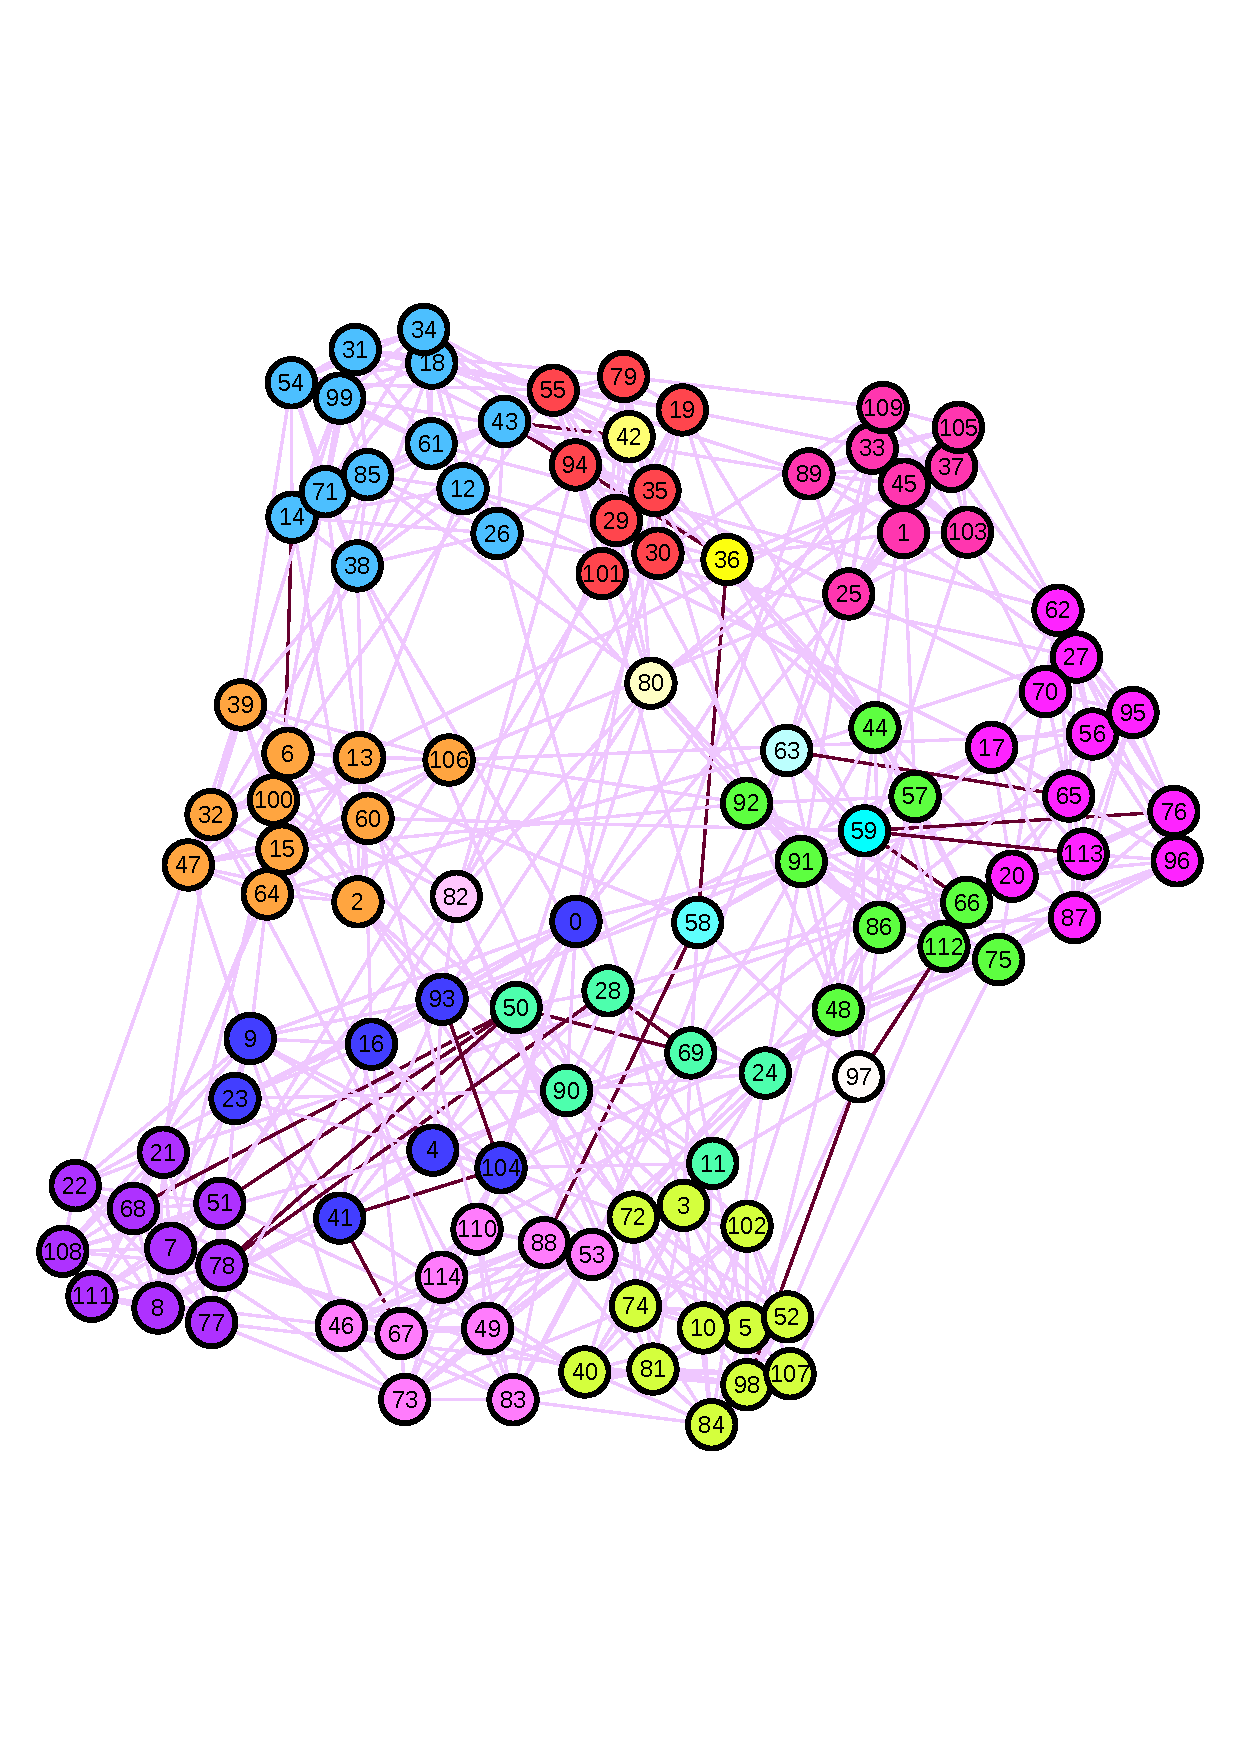
\includegraphics[width=.99\linewidth]{img/chap2/football_neg_edge.pdf}
\caption{}\label{fig:football_groundtruth}
\end{subfigure}
\begin{subfigure}{.3\textwidth}
\centering
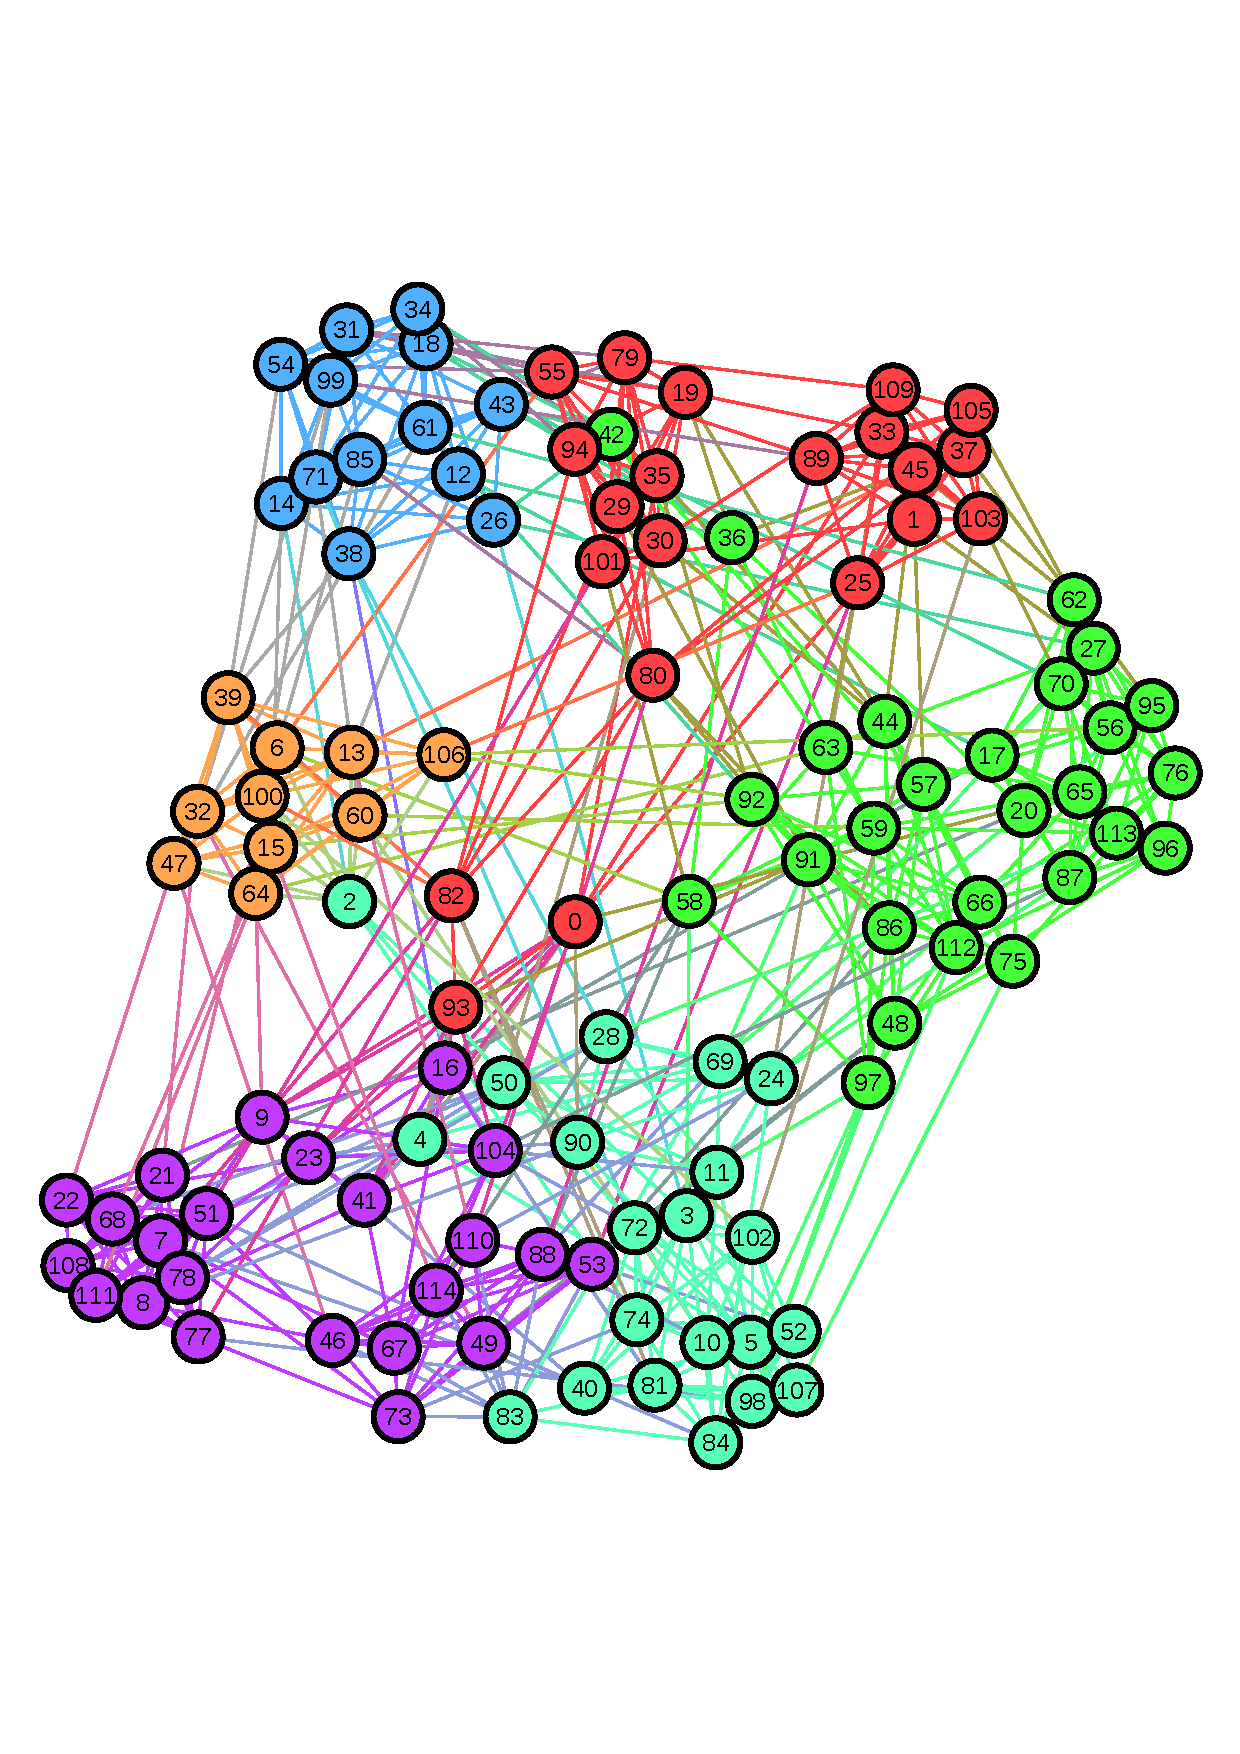
\includegraphics[width=.99\linewidth]{img/chap2/football_orig.pdf}
\caption{}
\label{fig:football_orig}
\end{subfigure}
\begin{subfigure}{.3\textwidth}
\centering
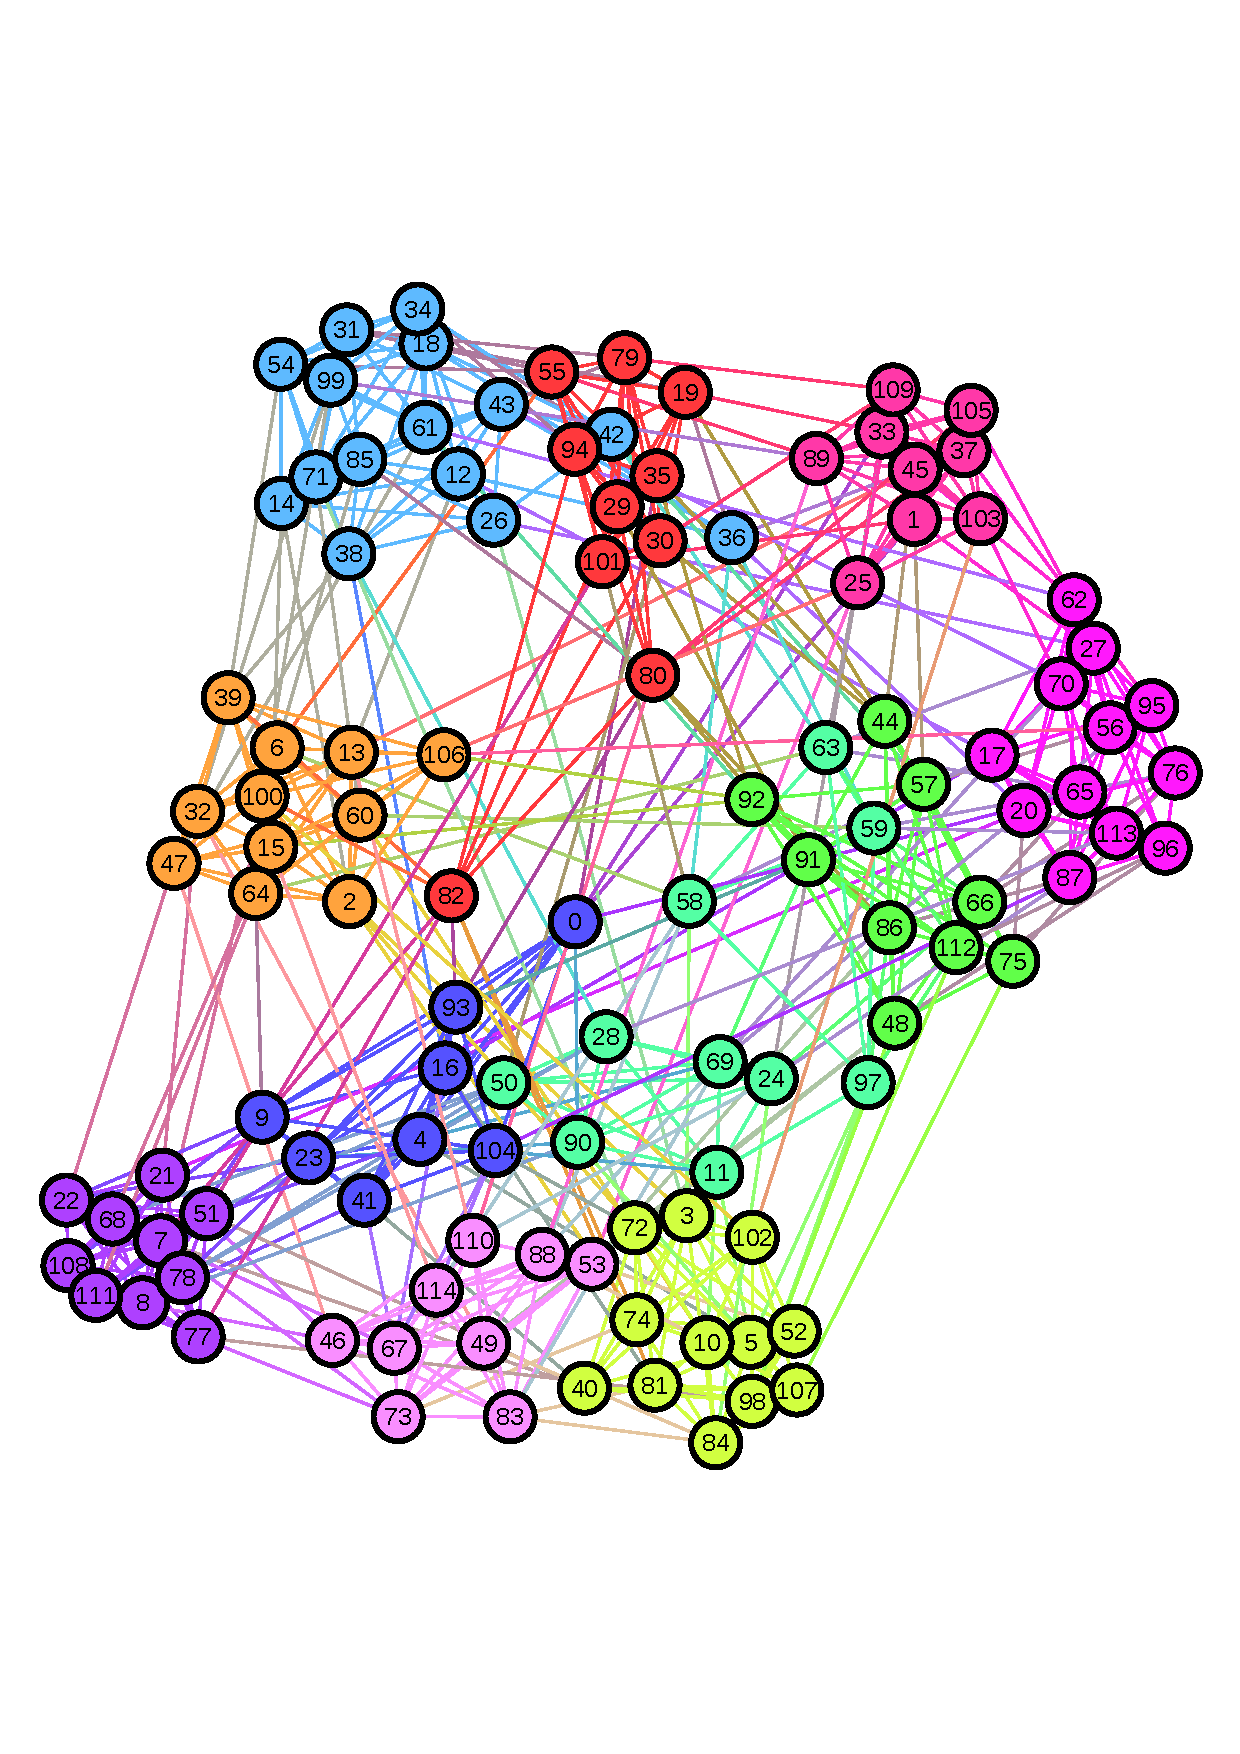
\includegraphics[width=.99\linewidth]{img/chap2/football_better.pdf}
\caption{}
\label{fig:football_better}
\end{subfigure}
\caption{The communities detected by the Fast Greedy algorithm~\cite{clauset2004finding} in the American college football network~\cite{evans2010clique}. Nodes are colored according to communities to which they have been assigned. (a) 19 ground truth communities defined as 11 conferences and 8 independent teams. Edges in black are assigned negative weights by the edge weighting scheme. (b) 6 communities detected on the unweighted graph by the modularity maximization method. (c) 11 communities detected on the weighted graph by the modularity maximization method.}
\label{fig:football_convergence}
\end{figure}
\textbf{American college football network} \label{sec:football}
The American college football network~\cite{evans2010clique} consists of 115 nodes representing college football teams playing in a league with 11 conferences. Two teams are linked if they have played with each other in the year 2000 season. The teams in each of the 11 conferences can be treated as one community because they play with each other often. There are 8 independent teams (not members of any conference), each forming a single community. 19 ground truth communities are shown in Figure~\ref{fig:football_convergence}.a with each color representing a single community. However, only 6 communities are detected by the Fast Greedy algorithm on an unweighted graph as shown in Figure~\ref{fig:football_convergence}.b because some adjacent ground truth communities are joined together.
\begin{table}[!t]
\caption{Metric values characterizing the community structures computed over the original unweighted American college football network but discovered in either the original unweighted graph or the corresponding weighted graph produced by our model.}
\label{table:football}
\centering
\setlength\tabcolsep{2pt}
\begin{tabular}{ |c|c|c|c|c|c|c| }
 \hline
Metric & Graph & FG & LE & LP & RW & ML \\
 \hline
 \multirow{2}{*}{NMI} & Original &0.58528&0.58140&0.76962&0.83833&0.83391\\
 & Weighted & 0.91117&0.85903&0.92635&0.91117&0.87272\\
\hline
 \multirow{2}{*}{ARI} & Original &0.49333&0.49441&0.71749&0.86938&0.85815\\
 & Weighted &0.94723&0.88982&0.91539&0.94723&0.90085\\
 \hline
 \multirow{2}{*}{$Q$} & Original &
 0.56860&0.49326&0.57668&0.60337&0.60503\\
 & Weighted & 0.60140&0.59338&0.57315&0.60140&0.60356\\
 \hline
 \multirow{2}{*}{$Q_{ds}$} & Original &0.15877&0.13661&0.21106&0.23650&0.23626\\
 & Weighted &0.25696&0.23893&0.24025&0.25696&0.24889\\
 \hline
\end{tabular}
\end{table}
The regression model converts the original unweighted graph to a weighted graph where the edges with negative weights are marked in black in Figure~\ref{fig:football_convergence}.a. On the weighted graph, the Fast Greedy algorithm can find 11 league communities, each containing one individual conference, although it allocates the independent teams to some of these league communities. The regression model is trained by sampling the ground truth communities on the artificial SBM network, which is constructed to be similar to the Football network. The training process takes approximately 10 seconds on a machine with a single 2.5GHz CPU.
Table~\ref{table:football} lists the results of the followings approaches: Fast Greedy algorithm~\cite{clauset2004finding} (FG), leading eigenvector method~\cite{newman2006finding} (LE), label propagation algorithm~\cite{raghavan2007near} (LP), community detection based on random walks~\cite{pons2005computing} (RW), multilevel algorithm~\cite{blondel2008fast} (LW) measured by the normalized mutual information (NMI) and adjusted rand index (ARI). As illustrated in Table~\ref{table:football}, in addition to the Fast Greedy modularity maximization algorithm, the state-of-the-art community detection algorithms, including label propagation algorithm by Raghavan et al.~\cite{raghavan2007near}, Newman's leading eigenvector method~\cite{newman2006finding}, the algorithm based on random walks~\cite{pons2005computing} and the multilevel algorithm by Blondel et al.~\cite{blondel2008fast}, also demonstrate improved performance on weighted graphs produced by our method\footnote{In the experiments, the edges with negative weight are removed from the graph because some community detection algorithms are not able to handle negative weights due to the algorithm design or implementation.}. This result additionally supports our claim that properly weighting a graph can lead to an improved quality of community detection.
For a fair comparison, regardless of whether the partition of the graph is determined with or without the edge weights, both the modularity $Q$ and modularity density $Q_{ds}$ are computed over the unweighted graph, i.e., edge weights are all set to 1. Hence, a better $Q$ or $Q_{ds}$ found on the weighted graph indicates the edge weights allow the maximization algorithm to avoid the inferior local optima. The NMI and ARI measures indicate that the communities detected in the weighted graph are generally accurate. However, from the aspect of modularity, for three algorithm, LP, RW and ML, such communities may be evaluated as inferior (as they have slightly lower modularity) than the communities discovered in the original unweighted graph. Consequently, even if the maximum modularity is reached in the original unweighted graph, the resulting communities are still not likely to match the ground truth. In contrast, the modularity density $Q_{ds}$\footnote{Note that the modularity density values are all computed over the original Football network.} of the communities detected in the weighted one is higher than in the original unweighted graphs, which means that it accurately measures the quality of these communities. The proposed edge weighting scheme leads to a higher modularity density $Q_{ds}$ in all cases because the weighted edges allows the greedy algorithm to escape from local maximum of $Q_{ds}$ and get better value of it on the original unweighted graph. 
\begin{figure}[ht!]
\centering
\begin{subfigure}{.45\textwidth}
\centering
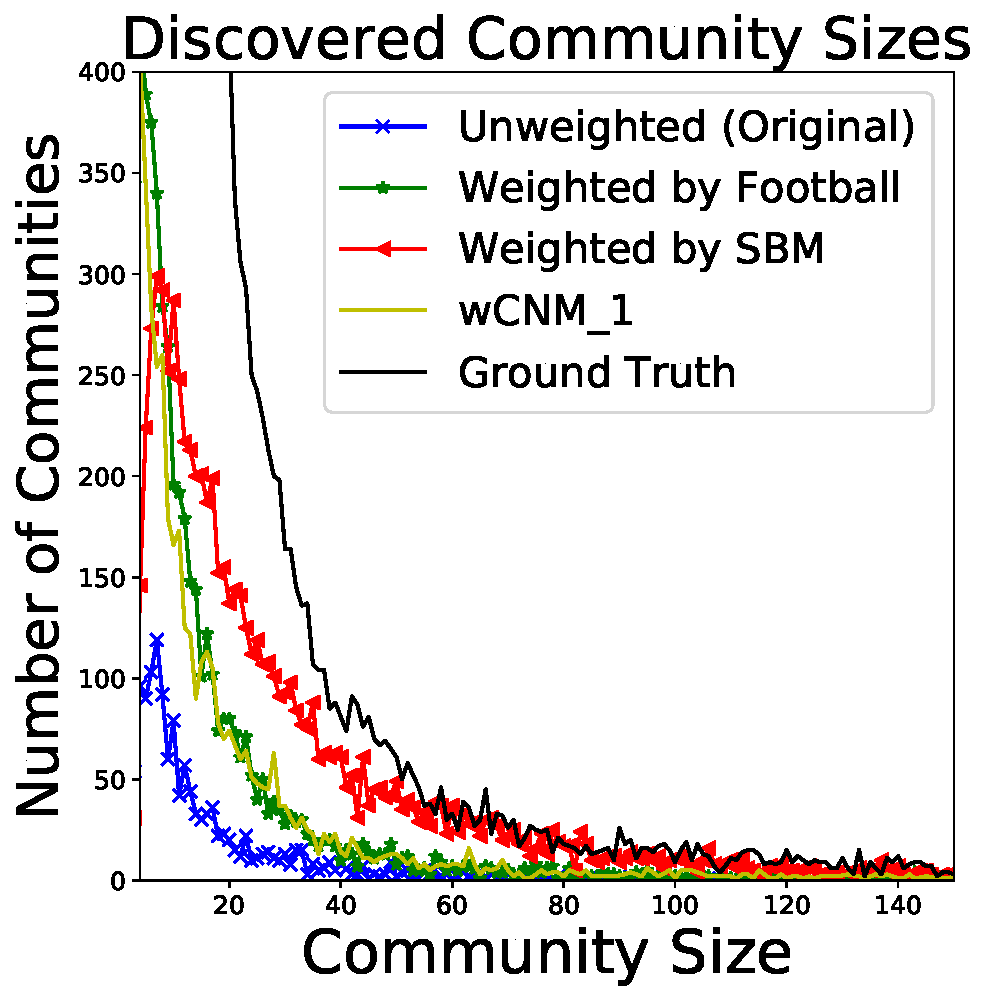
\includegraphics[width=.9\linewidth]{img/chap2/comm_distribution_amazon.pdf}
\caption{Amazon}
\label{fig:1}
\end{subfigure} %    <-- % added here
\hfill %% useful if width of each figure is less the .5\textwidth
\begin{subfigure}{.45\textwidth}
\centering
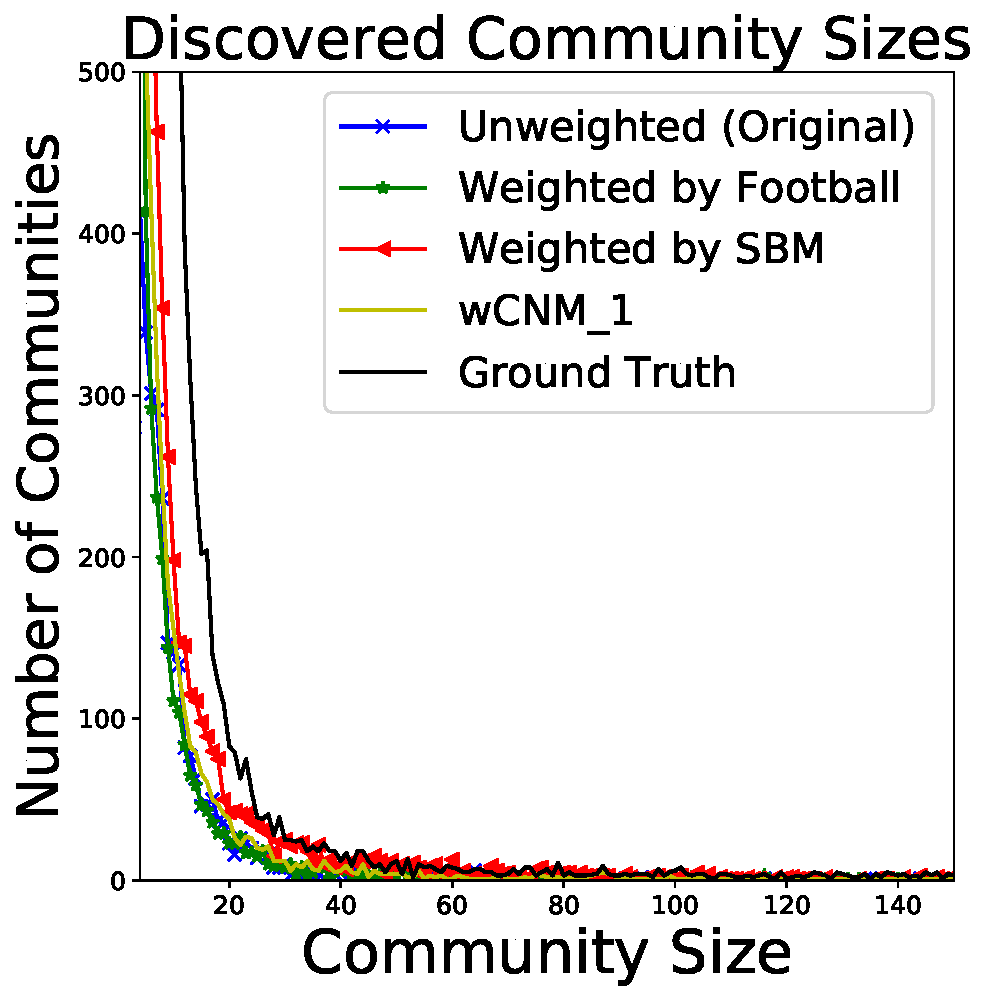
\includegraphics[width=.9\linewidth]{img/chap2/comm_distribution_dblp.pdf}
\caption{DBLP}
\label{fig:2}
\end{subfigure} \\
\begin{subfigure}{.45\textwidth}
\centering
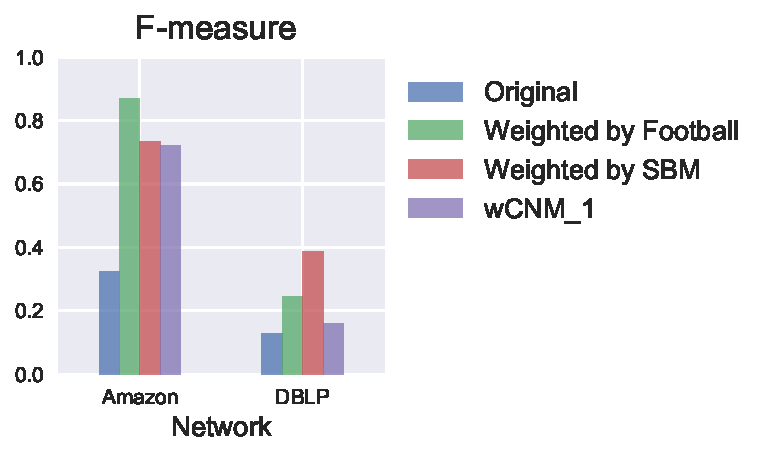
\includegraphics[width=.99\linewidth]{img/chap2/fmeasure.pdf}
\caption{F-measure}
\end{subfigure} %    <-- % added here
\hfill %% useful if width of each figure is less the .5\textwidth
\begin{subfigure}{.45\textwidth}
\centering
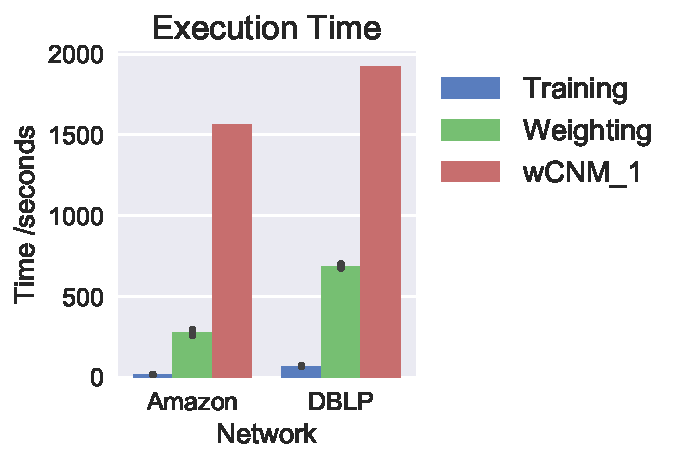
\includegraphics[width=.99\linewidth]{img/chap2/execution_time.pdf}
\caption{Efficiency}
\end{subfigure} \\
\caption{Performance improvement of community detection in Amazon and DBLP networks.}
\label{fig:comm_distribution}
\end{figure}
\textbf{Large Networks} We evaluate the performance of our model on two large real networks: Amazon co-purchasing network and DBLP co-authorship network. The Amazon co-purchasing network~\cite{yang2015defining} consists of 334,863 products with two frequently co-purchased products linked by an undirected edge. Each collection of products from the same category forms one ground-truth community. The DBLP collaboration network~\cite{yang2015defining} is the co-authorship network where every node represents a researcher. Two researchers who published at least one paper together are linked. Following others, we assume that individual ground-truth community is defined by the publication venue, e.g., journal or conference. 
The proposed weighting scheme is compared with the wCNM\_1 algorithm~\cite{berry2011tolerating} which computes the weight of an edge using all the triangles and 4-cycles containing it. In our experiments, the wCNM\_1 algorithm iterates only once over updates, because the results in~\cite{berry2011tolerating} show that additional iterations negligibly improve the final results. The regression model which converts the original unweighted graphs to weighted ones is trained by sampling the dynamically constructed artificial SBM networks. In addition, we also test the performance of our model trained by the ground truth communities in the American college football network, as shown in Figure~\ref{fig:comm_distribution}. Perhaps surprisingly, the accuracy of the modularity maximization algorithm on the weighted graph when weights were based on SBM artificial network has improved for the Amazon network by almost 50\% as measured by F-score and even more for the DBLP network. 
The sizes of communities discovered in Amazon and DBLP networks containing more than $3$ nodes are plotted in Figure~\ref{fig:comm_distribution}a-b. In the weighted graph produced by our model for the Amazon network, the distribution of the sizes of the detected communities is close to the distribution of the sizes of ground truth communities for weights based on SBM artificial network but quite different for weights based on the Football network. Since the F-score was similar for those two cases, this result demonstrates the importance of inspecting the distribution of the community sizes. In case of the DBLP network, the improvement of F-score is significant for the weights based on the SBM network, but the distribution of the community sizes is different. We believe that these two results show that presumed ground truth communities in DBLP are not correct, and that smaller communities of researchers co-authoring papers across several venues are the right communities. These results show that our model successfully converts large networks to the weighted ones where the modularity maximization algorithms can perform better than they do on the original unweighted networks.
In general, these large networks can be processed in a few minutes as shown in Figure~\ref{fig:comm_distribution}d. The computation time is divided into two parts: (i) Training: the time spent to infer all the parameters of the regression model; (ii) Weighting: the time needed to compute the weights of every edge in the graph. Both steps include the I/O processing time of loading the network files from disk. The edge topological feature extraction (i.e., weighting) time increases as the number of edges grow, therefore processing of dense graphs can be more time-consuming. Unlike the weighting time, the training time does not change much with the size of the original network. This is because the size of the constructed artificial network is independent of the size of the original input graph. Last but not least, in our experiments, the edge topological feature extraction and edge weight evaluation use a single thread implementation. However, as problems that are easily parallelizable, they can be partitioned into many individual tasks to achieve a better performance.


\section{Conclusions} \label{sec:2.7}
Modularity maximization is one of the state-of-the-art approaches for community detection in complex networks. However, due to the resolution limit problem, it tends to merge small, well-formed communities into a large component to increase the modularity. To deal with the resolution limit problem, we propose two key enhancements to the modularity maximization - one assigning proper weights to edges in the network; the other recursively dividing a graph into subgraphs until the remaining communities are statistically significant. The experimental results show that both approaches significantly improves the quality of the detected communities in the real and synthetic networks.

Besides the contributions on the practical community detection algorithms, we also develop the theoretical results for modularity-based community detection. Specifically, we establish the asymptotic lower and upper bounds of the generalized modularity. The lower bound corresponds to the highest background inter-community edge density in a network, while the upper bound corresponds to the lowest intra-community edge density. This work connects the resolution limit of modularity with random graph theories, which also reveals the ``plateaus" problem that no universal resolution parameter exists to detect all centers. The issue is analogous to finding mountains that are located at different plateaus; using a single altitude either would miss the lower mountains, or would treat the higher peaks as one mountain.

The stochastic block model can produce a wide variety of different network structures, including traditional assortative communities and different from them disassortative structures. In theory, it should be possible to guide the inference algorithm which type of structure is preferred when both types of structures fit the stochastic block model and its degree-corrected variant well for the input network. However, the existence of multiple local optima of the log-likelihood traps the inference algorithms in one of them. We apply a simple yet effective constraint on nodes' internal degree ratio of the degree-corrected stochastic block model. The resulting algorithm reliably finds assortative or disassortative structure as directed by the value of a single regularization parameter. We validated the model experimentally testing its performance on several real and synthetic networks.

Future works include applying more capable models as the nested hypothesis in the significance testing framework and extending the multi-scale community detection algorithm and edge weighting scheme to directed networks.


\chapter{INFORMATION PROPAGATION AND VIRALITY PREDICTION} \label{sec:2}

\let\thefootnote\relax\footnotetext{
Portions of this chapter previously appeared as:}
\let\thefootnote\relax\footnotetext{X. Lu, and B.~K. Szymanski, ``Towards limited scale-free topology with dynamic peer participation,'' {\em Computer Networks}, 2016.
}
\let\thefootnote\relax\footnotetext{
X. Lu, and B.~K. Szymanski, ``Predicting viral news events in online media,'' {\em IEEE International Parallel and Distributed Processing Symposium Workshops}, 2017.
}
\let\thefootnote\relax\footnotetext{
X. Lu, and B.~K. Szymanski,
``Scalable prediction of global online media news virality,'' {\em IEEE Transactions on Computational Social Systems}, 2018.}


%%% INTRODUCTION
\section{Introduction}
With the rise of online medium sites such as Facebook and Twitter, information propagation in these platforms attracts the interests of many researchers. Understanding the information propagation in these systems does not only provide better insights into the underlying sociology but is also crucial for the prediction of emergent social, economic and political phenomena. In the previous section, we study the detection of community structures in the complex network. In contrast, here, based on the topological features, we seek to predict the virality of cascades over the information propagation networks.

The mutual excitations between network nodes are widely observed in a variety of networks, ranging from the diffusion of purchasing behavior among friends to the spread of contagious disease. In a social network, information propagation can also be explained by the mutual excitations between individuals. Many previous works~\cite{weng2014predicting,zhao2015seismic,guille2012predictive} model the information diffusion as epidemics on networks - the acceptance of information is viewed as an infection of a node by infected neighbors in the network. These works assume that there exists an explicit propagation pathway which is sufficient to explain the observed information diffusion~\cite{yang2015defining} - messages can only spread along the predefined edges between nodes. In this section, we adopt these assumptions and develop efficient algorithms to predict the viral information propagation at its early stage.

As shown in~\cite{nematzadeh2014optimal}, strong community structures in a network enhance the local, intra-community spreading. This phenomenon is supported by the observations in online media: most news events are reported by the online news sites in the same region, using the same language. We exploit such community structures to parallelize the derivation of node embeddings because most cascades occur in local communities. In Section~\ref{sec:3.2}, according to the frequency of co-occurrence in cascades, the nodes in a network are divided into multiple communities in which the propagation occurs frequently. Every node in the propagation network has two latent vectors, one representing its influence to other nodes on different topics and the other representing its selectivity upon the inputs from other nodes on different subjects~\cite{bogdanov2014modeling}. Such latent representations of the influence and selectivity are analogous to the node's vector representation in the non-negative matrix factorization approach~\cite{lee2001algorithms,psorakis2011overlapping,yang2013overlapping}, where the inner product of two vectors indicates the strength of the connection between the corresponding nodes. These node embeddings are then used as input to predict the size of cascades. Unlike~\cite{gomez2013structure}, we represent the possible parameters of one link by the influence and selectivity of its two endpoints, which reduces the number of possible parameters and permits an efficient parallel algorithm to infer them. 

In Section~\ref{sec:3.2}, we propose a scalable community-based probabilistic framework to model the spreading of news about events in online media. News reports shape the public perception of the critical social, political and economic events around the world. The way in which emergent phenomena are reported in the news makes the early prediction of such phenomena a challenging task. Our approach exploits the latent community structure in the global news media and uses the affiliation of the early adopters with a variety of communities to identify the events widely reported in the news at the early stage of their spread. The time complexity of our approach is linear in the number of news reports. It is also amenable to efficient parallelization. To demonstrate these features, the inference algorithm is parallelized for message passing paradigm and scales well on RPI Advanced Multiprocessing Optimized System (AMOS), one of the fastest Blue Gene/Q supercomputers in the world. Thanks to the community-level features of the early adopters, the model gains an improvement of 20\% in the early detection of the most massively reported events compared to the feature-based machine learning algorithm. Its parallelization scheme achieves orders of magnitude speedup.

The scale-free topology has some good properties to facilitate information propagation, including high tolerance to random attacks\cite{albert2000error}, high synchronizability\cite{korniss2007synchronization} and resistance to congestion\cite{toroczkai2004network}. For this reason, several growth models are proposed to construct the scale-free overlay topology. The BA model\cite{barabasi1999emergence} manages to explain the evolution of scale-free topologies by a core principle named ``Preferential Attachment'' which means a new node is more likely to connect to heavily linked nodes when it joins the network. However, it is not practical in real distributed applications because the global information is required to maintain the degree distribution. Therefore, a distributed approach that constructs the topology without global information is desired.

In Section~\ref{sec:3.3}, we propose a distributed algorithm to construct limited scale-free networks which are robust against the traffic congestion and network failures~\cite{lu2016towards}. We compare our approach with other P2P network construction algorithms including HAPA\cite{guclu2009limited}, Gaian\cite{bent2008dynamic} and SRA\cite{bulut2014constructing} algorithms which construct the scale-free overlay topology with partial or no global information. The results show that our approach can maintain a scale-free overlay network while the other approaches are often vulnerable to dynamical peer participation. 

\section{Scalable prediction of global online news} \label{sec:3.2}

\subsection{Datasets} \label{sec:3.2.1}
We investigate the news data in the Global Database of Events, Language, and Tone (GDELT)\footnote{http://www.gdeltproject.org/} project. The GDELT project provides real-time news events extracted from tens of thousands of online news sites around the globe. Advances in natural language processing allows the sentiment analysis, real-time translation of 65 languages and the identification in events data of named entities including organization, location, count and theme. The dataset is currently available on Google Cloud Platform. Users can use Google BigQuery to download specific tables or process the data remotely by SQL commands. The GDELT database contains records the mentions of news events by news sites since February 19, 2015 to present. Here we present some unique features explored in these records. 

\begin{itemize}
\item \textbf{Emergence of news events}.
We calculate the duration of events, computed as the period since its earliest record until the latest. Most news events are reported by the news site within the first 50 hours. This reflects the short life cycle of the production and consumption of the news events. One explanation for this phenomenon is that a news site would prefer not to report an event which is considered out-of-date. In contract to the breaking news, the discussion of long-term topics such as greenhouse effect lasts a very long time, but these events constitute a very small portion of the dataset.

\begin{figure}[t!]
\centering
\begin{subfigure}{.5\textwidth}
\centering
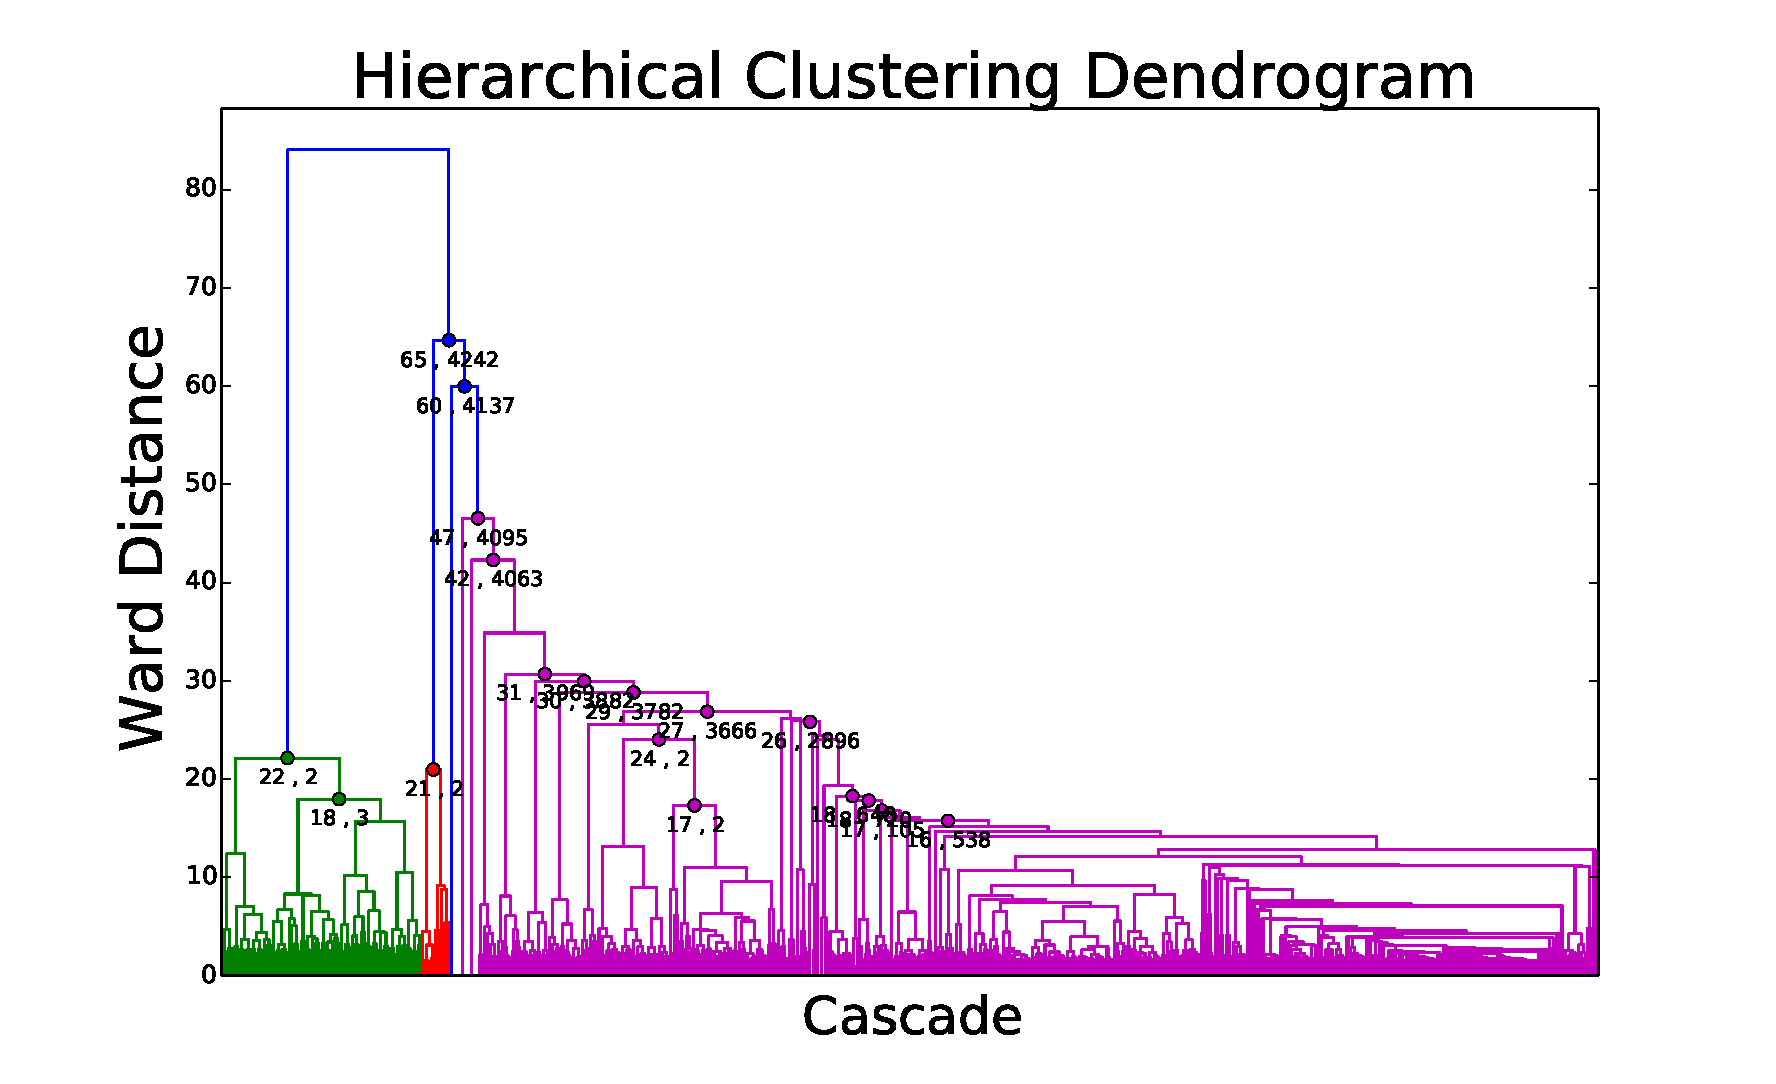
\includegraphics[width=.99\linewidth]{img/chap3/dendro.pdf}
\caption{Dendrogram of hierarchical clustering of the 5,000 random cascades of news events} \label{fig:dendro}
\end{subfigure}
\begin{subfigure}{.45\textwidth}
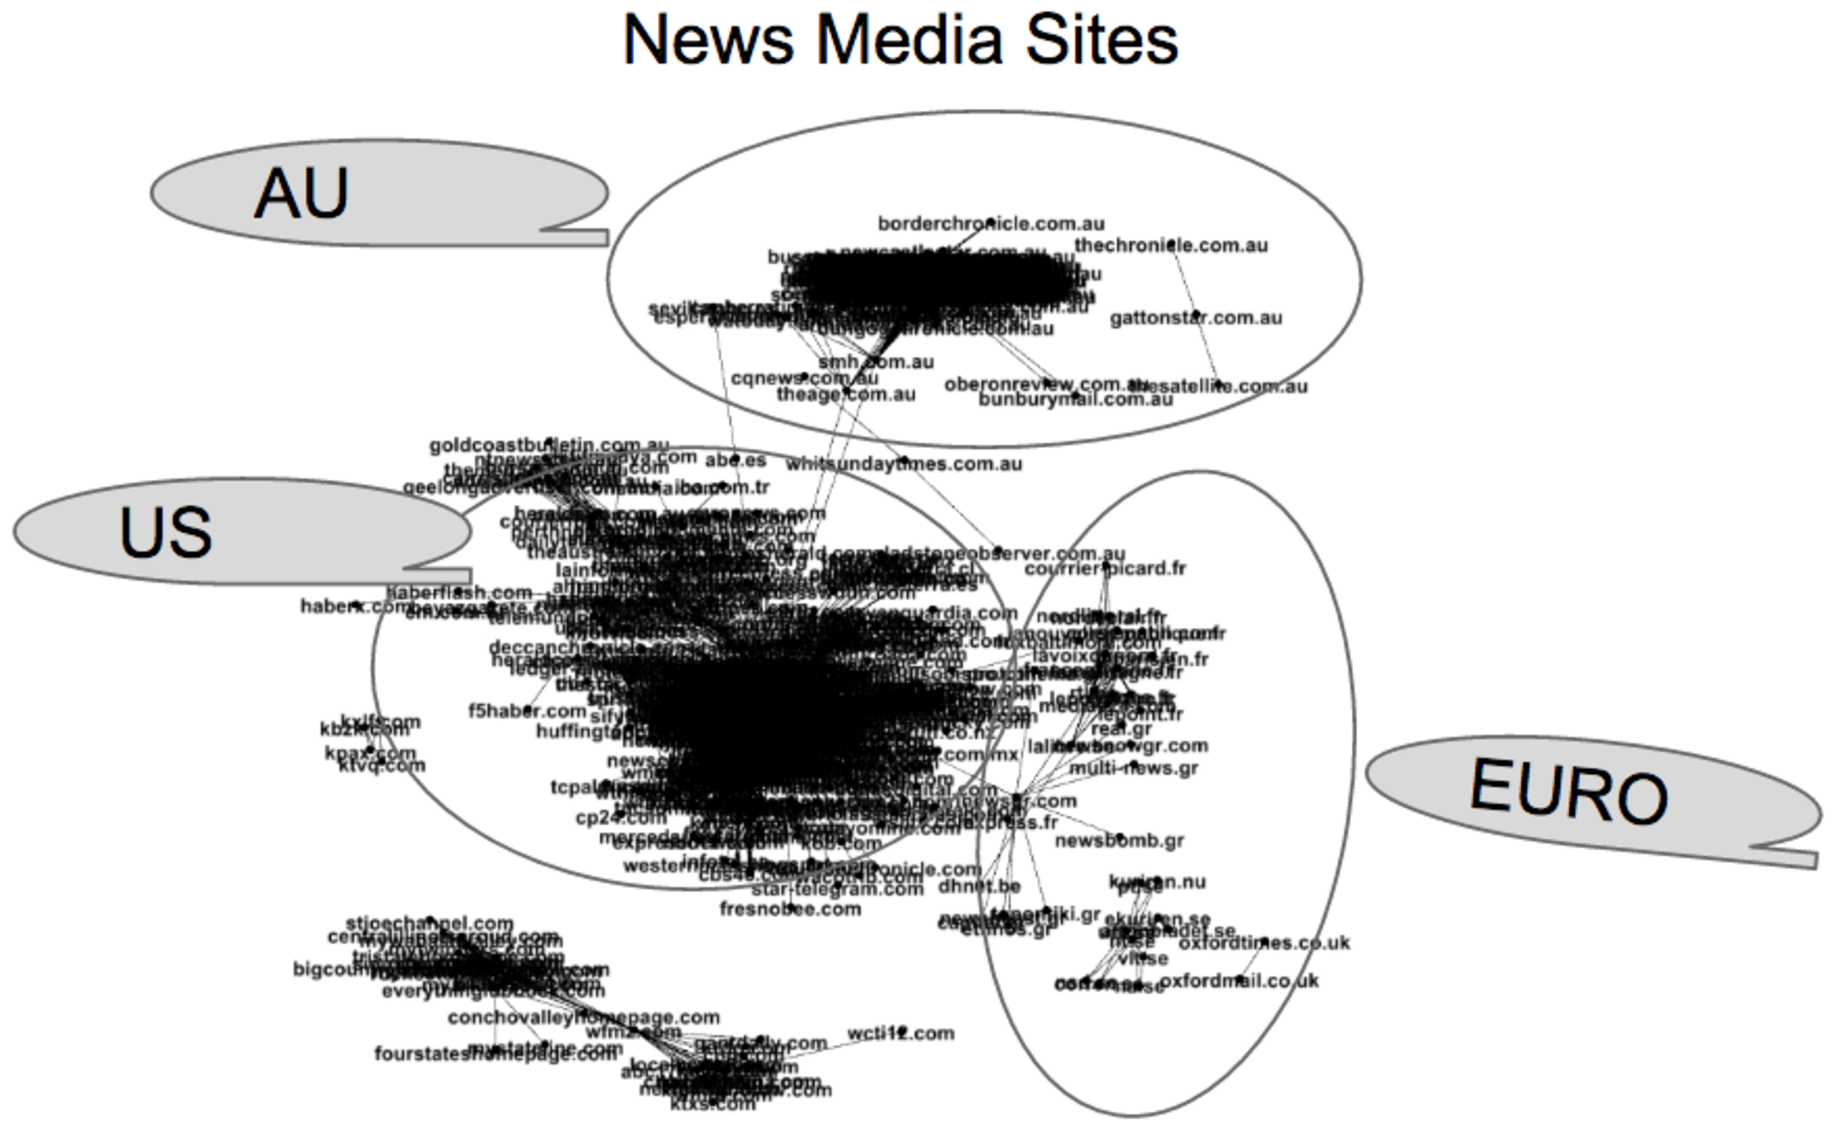
\includegraphics[width=.99\linewidth]{img/chap3/news_sites_graph.pdf}
\caption{Backbone network of the news sites associated with the 5,000 sampled cascades of news events} \label{fig:backbone}
\end{subfigure}

\caption{The hierarchical structure of online media and the backbone co-reporting network.}
\end{figure}

\item \textbf{Most cascades are local}. 
For a period covering one year, we randomly choose 5,000 news events in the GDELT dataset. Any two news sites reporting at least 50 events together are linked in the graph shown in Figure~\ref{fig:backbone}. Clearly, there are four clusters visible in Figure~\ref{fig:dendro}, one standing for the news sites in the U.S., one for the news sites in Australia and the other for the news sites in European countries, while the remaining one is a mixture of sites in different regions. Initially, the pair-wise distance between any two cascades of events is measured by the Jaccard-index
\begin{equation}
    \text{Jaccard} = \frac{|N(i)\cap N(j)|}{|N(i)\cup N(j)|}
\end{equation}
where $N(j)$ is the set of news sites reporting the news event $j$. Then the hierarchical clustering algorithm~\cite{johnson1967hierarchical}, which merges iteratively the closest cascades according to the Ward distance measure among all pairs of cascades, is applied to obtain a dendrogram as shown in Figure~\ref{fig:dendro}. The Ward distance and the number of cascaded contained in a cluster are also plotted in text at some associated inner nodes of the clustering tree. There are three obvious clusters shown in the dendrogram. The largest cluster in blue corresponds to the news sites in the U.S., while most news sites in Australia are located in the middle cluster in green. The news sites in U.K. and European countries are placed in the left-most cluster in red. Although the plot shows only a raw distribution of the news site in different clusters, the dual visualization indicates that the hierarchical structures of cascades correlate with the community structure of co-reporting networks of the news sites. That is, as an illustrative example here, most cascades of news events occur frequently within certain regions only.

\item \textbf{Matthew effect in online media}.
The term  Matthew effect (or accumulated advantage) originated in sociology and refers to a phenomenon in which ``the rich get richer and the poor get poorer.'' In network science, it refers to preferential attachment of earlier nodes in a network~\cite{barabasi1999emergence} where nodes that few nodes that acquire more connections than others will increase its connectivity at a higher rate while others have few connections. As seen in Figure~\ref{fig:popularity}, the distribution of the number events reported per site follows the Power Law, which has been widely observed in a variety of networks. As shown in Figure~\ref{fig:popularity}, only a few popular news sites have reported millions of events, while most of the news site reported 5,000-10,000 events. In the Figure~\ref{fig:popularity}, the news site which reported less than 5,000 events in one year are ignored because they are less influential than the remaining ones. The goodness-of-fit is measured by the p-value as shown in Figure~\ref{fig:popularity_pvalue}.

\begin{figure}
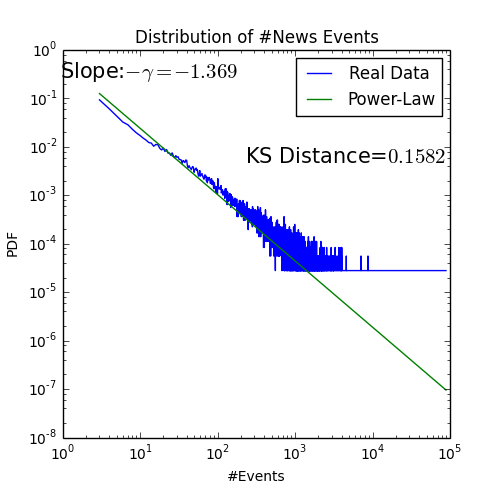
\includegraphics[width=0.46\textwidth]{img/chap3/histo.png}
\centering
\caption{The distribution of the number of events reported by the news sites follows the power law.}\label{fig:popularity}
\end{figure}

\begin{figure}
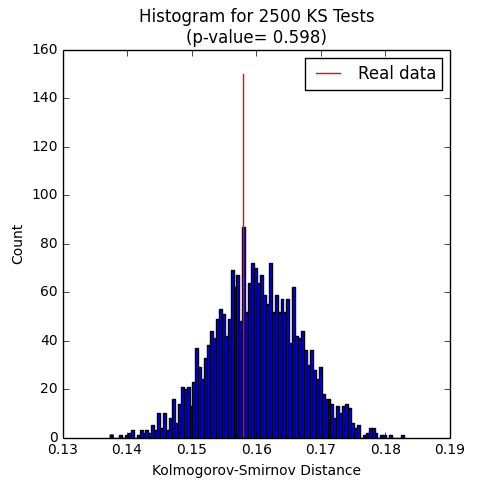
\includegraphics[width=0.46\textwidth]{img/chap3/histo_pvalue.png}
\centering
\caption{Goodness of fit measured by the p-value}\label{fig:popularity_pvalue}
\end{figure}
\end{itemize}
    
We also generate \textbf{synthetic information cascades} to evaluate the performance of the prediction algorithms proposed in this section. The networks are generated using the Stochastic Block Models as discussed in Section~\ref{sec:2.2.2}. Given the membership of all the $n$ nodes, the edge with two endpoints in different communities is created with the probability $\beta$ and the edge inside a community is created with probability $\alpha$. In most cases, $\alpha$ is much larger than $\beta$, so the graph contains the dense intra-community structures and sparse  inter-communities structures. We create the SBM graphs containing 2,000 nodes with $\alpha=0.2$ and $\beta=0.001$. The average degree of nodes is approximately 10. Each community in SBM graph contains approximately $40$ nodes.

On each network instance, the spreading process is simulated according to the stochastic propagation model proposed by Kempe et al.~\cite{kempe2003maximizing}. Since any cascade would eventually flood the entire network, we set an observation window during for the cascades. After the observation window, the current spreading process will be terminated instantly and a random node is chosen as the initiator to start the simulation of the next cascade. A total of 3,000 cascades are collected for each graph instance. The first 2,000 cascades are used to infer the influence and selectivity vectors of nodes in the network and the last 1,000 cascades are used to test the accuracy of the virality prediction algorithm. For the last 1,000 cascades, the infections occurring in the first 2/7 time of the observation window are provided for the prediction task, while the remaining parts of infections are assumed to be unknown.

More formally, the infection delay of $v$, i.e. $t_v$, can be treated as a random value
\begin{equation}
\begin{array}{rcl}
   &t_v = \min{t_{u_1}, t_{u_1},\dots,t_{u_r}} \\
   &\forall i \in [1,r] \quad : \quad t_{u_i} \sim \mathcal{K}(\alpha_{u_i,v})
\end{array}
\end{equation}
where $t_{u_i}$ is the infection time of the $i$-th neighbors of node $v$, $\alpha_{u_i,v}$ is a parameter associated with the edge $(u,v)$ in the propagation network and $\mathcal{K}()$ is the distribution of infection delays. In our experiments, $\mathcal{K}()$ is set as the exponential distribution which is observed in many social dynamics~\cite{barabasi2005origin}, and we set $\forall (u,v)\in E$: $\alpha_{u,v}=1$ for simplicity. In theory, the IC model supposes the entire network will be infected given a sufficiently long period. Since contagions generally do not infect all the nodes in the network, in our experiments the simulation of every cascade happens within a predefined observation window~\cite{gomez2013structure}.

\subsection{Community affiliation model for information cascades}
Community structures are widely observed in a variety of networks. Based on patterns of news about events spreading in the online news media, we present two basic observations below: 
\begin{itemize}
    \item Most news sites have a preference for the topics of their news coverage, e.g. politics, finance, education, military, technology or sports.
    \item The news reports are usually confined to the geographical and cultural boundaries. Although many media companies have ambitions to have global market presence, most media sites have only a regional reach~\cite{hjarvard2001news}.
\end{itemize}

Much like many community detection methodologies \cite{blondel2008fast,clauset2004finding,lu2017adaptive,xie2011community,fortunato2010community} which aim at discovering dense sub-graphs embedded in a network, we seek to recover such community structure for the online news sites. However, in the global and local news markets~\cite{leetaru2013gdelt}, connecting every two sites reporting the same event could result in an extremely dense network. Finding community structure in such network would not only incur high computational power but would also cloud the real connections among communities. Therefore, we find the latent community affiliation of these news sites rather than drawing the edges between specific news sites. Since the underlying network topology is unknown, our probabilistic model incorporates the time points of each infection in the observed news cascades, i.e., the time of each news report. Formally, we present the definition of information cascade below.

An information/news cascade is a set of infections $\{(u, t_u)\}$. Each infection $(u, t_u)$ consists of a node $u$ and its infection time $t_u$. Our model assumes the news cascades happen at the community level. For a particular community of news sites, the probability of a site reporting a particular news depends on both the affiliation of this news sites with the community and the probability of the news cascade reaching its community. To formalize this idea, we define latent community below.

A latent community is a set of nodes that, conditioned on the infection of one member, the probability that other members will get infected within a limited period is much higher than for the non-members. In \cite{yang2013overlapping}, authors propose a community affiliation model where each node has a probability belonging to one of the overlapping communities in the network. We extend this community affiliation model by taking into account the probability for each cascade to spread to these overlapping latent communities. As illustrated in Figure~\ref{fig:affiliation_model1}, if a cascade has a non-zero probability of spreading to a community, this cascade (square) is connected to the community (double circle); if a node (circle) belongs to a community, then this node is connected to the community as well. Our affiliation model captures two important features of cascades and communities in complex networks: (i) the community structures are highly overlapped, a node can belong to multiple communities at the same time; (ii) the members of the same community tend to accept similar information during the information cascades. 

\begin{figure}
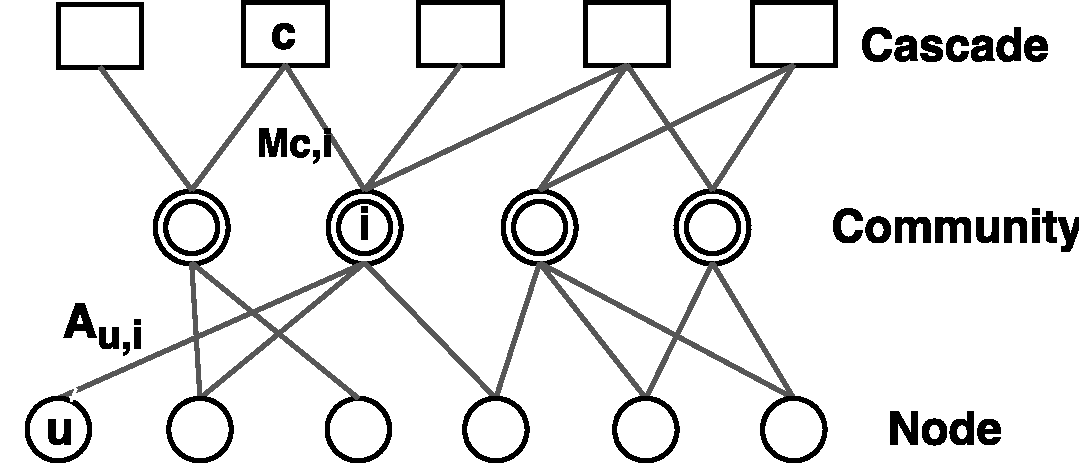
\includegraphics[width=.6\textwidth]{img/chap3/affiliation_model_V2.pdf}
\centering
\caption{Community affiliation model with cascades. Cascade $c$ belongs to the two leftmost communities, and node $u$ belongs to community $i$.}\label{fig:affiliation_model1}
\end{figure}

Social theories~\cite{barabasi2005origin} suggest that the response time of human beings usually follows the exponential distribution, which explains the burstiness of social behavior in many scenarios. Our analysis of 723,037 randomly sampled news reports shows that the delays of news reports also fit the exponential distribution with a high $R^2$ score of 92\%. We consider the news reports with a delay less than 21 hours, which comprise 99\% of the sampled data from the Global Database of Events, Language, and Tone (GDELT) dataset. Based on this observation, we model the response time of news sites to events by an exponential distribution.

For every single community $i$, let $A_{ui} > 0$ denote the strength of affiliation of node $u$ with it and $M_{ci} \in (0,1]$ denote the probability of the cascade spreading to community $i$. In this community, the response time of node $u$ to cascade $c$ follows the exponential distribution
\begin{equation} \label{eq:expo_ez}
t_u^c(i) \sim Exp(A_{u,i} M_{c,i})
\end{equation}
which indicates that the node $u$ gets quickly infected when the cascade $c$ is highly likely to reach a community $i$, i.e. $M_{c,i}$ is large, and the affiliation of $u$ with community $i$ is strong, i.e. $A_{u,i}$ is large.

Most real-world networks have overlapping community structures which allow a node to belong to many communities. Therefore, in our model, the response time of a node to a cascade corresponds to the minimum response time in all communities. Given a node $u$, a cascade $c$ and a total of $m$ overlapping communities, the minimum response time also follows the exponential distribution\footnote{The minimum of $m$ mutually independent random variables $X_i \sim Exp(\lambda_i)$ for $i=1,2,\dots,m$ also follows the exponential distribution, i.e. $min(X_i) \sim Exp(\sum_i\lambda_i)$.} 

\begin{equation} \label{eq:total}
\min \{ t_u^c(1),t_u^c(2),\dots, t_u^c(m) \} \sim  Exp(\sum_{i=1}^{m} A_{u,i} M_{c,i} ) 
\end{equation}
where the rate parameter is the sum of the rate parameters for each individual exponential distribution in Eq.~\ref{eq:expo_ez}.

In reality, news agencies usually have some bias for the content of information they spread. Such bias can be positive - there are certain types of information a news agency favors, while it can also be negative - messages of no interest to agency's audience are ignored or intentionally blocked. It is tempting to allow the value of $M_{c,i}$ to be negative for this reason so that the affiliation with some community may delay the response time of some node, i.e. $A_{c,i} M_{c,i} < 0$. However, it could result in a negative rate parameter $\lambda$ in Eq.~\ref{eq:total} which violates the constraint $\lambda > 0$ of the exponential distribution. Hence, we smooth the rate parameter via the sigmoid function $\sigma : \mathbb{R} \to [0,1]$. In this way, given an information cascade $c$, the response time of a node $u$, $t_u^c = \min  t_u^c(i)$, draws from an exponential distribution with a rate parameter $\gamma = w \sigma( A_u \cdot M_c)$,
\begin{align} \label{eq:sigmoid}
t_u^c \sim Exp(w \sigma(A_u \cdot M_c))
\end{align}
where $\sigma(x)= \frac{1}{1+e^{-x}}$ is the sigmoid function, $w$ is a scaling parameter and $\cdot$ represents the inner product in vector space, while the $i$-th component of vector $A_u$ and $M_c$ are  $A_{ui}$ and $M_{ci}$ respectively. Using the sigmoid function here avoids any constraint for the parameters $A_u$ and $M_c$, and most importantly, it improves the robustness of the parameter estimation because the sigmoid function is differentiable at each point. 

So far, the model takes into account the participants of a cascade. However, the nodes which are not involved in a cascade also provide information about their affiliations with different communities. Since these silent nodes are equivalently important, we set a upper bound on the response time, $T \gg t_u^c $ for $\forall u$ and $\forall c$, such that all the silent nodes during the cascading propagation can be assumed to have this long response time $T$.

Given an information cascade $c=\{(u_i^c, t_i^c) | i=1,2,\dots,n_c\}$ where the $i$-th node $u_i^c$ has response time $t_i^c$, the likelihood of observing a cascade $c$ is
\begin{equation} \label{eq:casc_likelihood}
L_c = \prod_{u\in V_c} p_{u,c}(t_u^c)  \prod_{u \notin V_c}  p_{u,c}(T)
\end{equation}
where $V_c = \{u_i^c | i=1,2,\dots,n_c\}$ denotes the set of nodes involved in cascade $c$ and $p_{u,c}(t)$ is the probability density function of the exponential distribution
\begin{equation} \label{eq:pdf}
p_{u,c}(t) = w\sigma( A_{u} \cdot M_c) e^{-w\sigma( A_{u} \cdot M_c) t}
\end{equation}
Since the likelihood $L_c$ is the product of $|V|$ terms, Eq.~\ref{eq:casc_likelihood} can be too expensive to compute. But it can be approximated by using a subset of representatives $D_c$ drawn randomly from $V\setminus V_c$. This idea is similar to the negative sampling approach~\cite{mnih2012fast}, which has been successfully applied to learning the distributed representation of words in documents~\cite{mikolov2013distributed,ji2016parallelizing}. The log-likelihood of an observed cascade then becomes
\begin{equation} \label{eq:neg}
\begin{array}{rcl}
   \mathcal{L}_c \approx & \sum_{u \in V_c} \log p_{u,c}(t_u^c) + \sum_{u\in D_c} \log p_{u,c}(T)
\end{array}
\end{equation}
where $D_c$ is the set of negative samples chosen for every cascade by drawing random nodes uniformly from $V$. If we fix the size of each $D_c$ as $d$, then a speedup of approximately $|V|/d$ times can be achieved.

To estimate the parameters $A_u$ for each $u$ and $M_c$ for each $c$, we maximize the likelihood which factorizes into the product of the likelihoods of $k$ cascades. This goal is equivalent to maximizing the sum of the log-likelihood of $K$ cascades
\begin{equation} \label{eq:loglikelihood}
\{\hat{A}_u\}, \{\hat{M}_c\} = \argmax_{\{A_u\}, \{M_c\}} \sum_{c=1}^{k} \mathcal{L}_c
\end{equation}
It is worth noting that the problem defined by Eq.~\ref{eq:loglikelihood} does not require explicit network topology to estimate $A_u$ and $M_c$. Instead, the input of the model is the response times of the nodes to every cascade. This is a practical setting when the underlying network topology is incomplete or hidden during the information propagation process. In addition, the parameter space $\{A_{ui},M_{ci}|\forall i,u,c\}$ in Eq.~\ref{eq:loglikelihood} does not have any restriction thanks to the adoption of the sigmoid function in Eq.~\ref{eq:sigmoid}.

The optimization problem in Eq.~\ref{eq:loglikelihood} is unfortunately not convex. Since the network size can be large, the optimization problem involves a large number of parameters, which makes stochastic updates more suitable than the batch methods. In addition, when some new cascade data comes in, the estimation algorithm should be able to incorporate the new cascades efficiently. For these reasons, we apply the Stochastic Gradient Ascent (SGA) method to estimate the parameters.

If we substitute Eq.~\ref{eq:neg} into Eq.~\ref{eq:loglikelihood}, the partial derivative of the objective function $F$ in Eq.~\ref{eq:loglikelihood} over a particular $M_c$ becomes 
\begin{equation} \label{eq:partial}
    \frac{\partial F}{\partial M_c} =  \sum_{u\in V_c} \frac{\partial \log p_{u,c}(t^c_u) }{\partial M_c} + \sum_{u\in D_c} \frac{\partial \log p_{u,c}(T) }{\partial M_c}
\end{equation}
which is a weighted sum of the terms in the form of $\frac{\partial \log p_{u,c}(t) }{\partial M_c}$. Given the value of $t$, $p_{u,c}(t)$ depends only on $A_u$ and $M_c$. The partial derivative of $\log p_{u,c}(t)$ over $M_c$ can be computed using $A_u$ and $M_c$
\begin{equation} 
    \frac{\partial \log p_{u,c}(t)}{\partial M_c} = \big[1 - \sigma( A_u \cdot M_c) w t\big] \big[1-\sigma( A_u \cdot M_c)\big] A_u
\end{equation}
Here we need the $A_u$ for $\forall u \in V_c \cup D_c$ to update $M_c$ according to the gradient in Eq.~\ref{eq:partial}. Similarly, the partial derivative of the objective function $F$ in Eq.~\ref{eq:loglikelihood} over $A_u$ can be computed using the $M_c$ for cascades $c$ such that $u \in V_c \cup D_c$
\begin{equation}
\frac{\partial F}{\partial A_u} =  {\sum_{c:u\in V_c}} \frac{\partial \log p_{u,c}(t^c_u) }{\partial A_u} + {\sum_{c:u\in D_c}} \frac{\partial \log p_{u,c}(T) }{\partial A_u}
\end{equation}
where the term $\frac{\partial \log p_{u,c}(t)}{\partial A_u}$ depends on $A_u$ and $M_c$ only
\begin{equation} 
    \frac{\partial \log p_{u,c}(t)}{\partial A_u} = \big[1 - \sigma( A_u\cdot M_c) w t\big] \big[1-\sigma( A_u\cdot M_c)\big] M_c
\end{equation}
In this way, the parameters can be updated in a pair-wise manner: we fix $A_u$ for all $u$ and update all the $M_c$s, and then fix all $M_c$s to update $A_u$s in every SGA iteration. The SGA updates can operate on a bipartite graph where node $u$ and cascade $c$ are connected if $u\in V_c \cup D_c$ (cf. the example shown in leftmost diagram in Figure~\ref{fig:pll}). To update $A_{u}$, each cascade $c$ propagates the corresponding parameters $M_c$ through the links in the bipartite graph to the node $u$. Then node $u$ calculates the partial derivative $\frac{\partial \log p_{u,c}(t) }{\partial A_{u}}$ for every connected cascade $c$ and updates $A_{u}$ accordingly. Similarly, the nodes can propagate the parameters $A_u$s through the links in this bipartite graph towards each relevant cascade $c$, and $M_{c}$ can be updated using the $A_u$ it receives. 

The pseudo code is shown in Algorithm~\ref{algo:sga1}.
The \textbf{time complexity} of each SGA iteration here is linear in the number of edges in the bipartite graph. This is because the loop in lines 8-19 iterates over all the nodes $u$ connected with each cascade $c$, which corresponds to visiting every edge of the bipartite graph exactly once. Similarly, the lines 20-31 also visit every edge in the bipartite graph once. In the news dataset, the number of edges of the bipartite graph is defined by the number of news reports, because every report connects a news site to a news cascade, plus the pair of negative samples edges $(u, c)$ for $u\in D_c$ with $|D_c|=d$ fixed as a constant. Hence, the time complexity of each SGA iteration is linear in the number of edges in the bipartite graph. The time complexity of Algorithm~\ref{algo:sga1} is also determined by the number of SGA iterations. In practice, this only involves tens of iterations before the derived $A_u$ and $M_c$ vectors become stable. Thus, this number can be treated as a constant. Therefore, the Algorithm~\ref{algo:sga1} has a linear time complexity in the number of bipartite graph edges, i.e. the number of news reports.


\begin{algorithm}
\caption{SGA Algorithm using a Single Processor}\label{algo:sga1}
\begin{algorithmic}[1]
\State $\alpha = \text{the SGA stepsize}$
\For {each cascade $c$} 
\For {each node $u \in V_c$}
\State $t_u^c = \text{infection delay of node $u$ in cascade $c$}$
\EndFor
\EndFor
\For {each SGA iteration}
\For {each cascade $c$} 
\For {each node $u \in V_c \cup D_c$}
\If {$u \in V_c$}
\State $t= t_u^c$
\ElsIf{$u \in D_c$}
\State $t= T$
\EndIf
\For {$i = 1,2,\dots,m$}
\State $A_{ui} \pluseq \alpha \frac{\partial \log p_{u,c}(t) }{\partial A_{ui}}$
\EndFor
\EndFor
\EndFor
\For {each node $u \in V$}
\For {each cascade $c$ such that $u \in V_c \cup D_c$}
\If {$u \in V_c$}
\State $t= t_u^c$
\ElsIf{$u \in D_c$}
\State $t= T$
\EndIf
\For {$i = 1,2,\dots,m$}
\State $M_{ci} \pluseq \alpha \frac{\partial \log p_{u,c}(t) }{\partial M_{ci}}$
\EndFor
\EndFor
\EndFor
\EndFor
\end{algorithmic}
\end{algorithm}

\subsection{Parallelization for distributed memory machines}
In practice, the input network size can be large so to speed up computation we offer parallelization of the parameter estimation for our model. Since the SGA algorithm is inherently sequential, many works including~\cite{ji2016parallelizing,mikolov2013distributed} use the Hogwild! framework~\cite{recht2011hogwild} attempting to parallelize the SGA algorithm on shared memory machines. The Hogwild! framework ignores the write-write conflicts caused by parallel updates on the same parameter as long as one unique processor can complete its writing operation. The quality of the results produced by SGA algorithm is guaranteed by the property that such conflicts are sparse enough. In the information diffusion context, however, such data sparsity is uncertain. To handle the contentions between processors, we propose a scalable parallelization scheme based on message passing paradigm~\cite{gropp1999using}.

The parallelization scheme is illustrated in Figure~\ref{fig:pll}. Consider eight nodes (blue) involved in eight cascades (yellow) in this toy example. The bipartite graph connects every pair of associated nodes and cascades in the SGA updates. These nodes and cascades are then distributed in this example to two processors. The first processor owns the upper four nodes and upper four cascades while the remaining nodes and cascades are assigned to the second processor. Each processor creates private memory space for the parameters of the nodes and cascades it owns. Much like Algorithm~\ref{algo:sga1}, the SGA algorithm propagates parameters back and forth between nodes and cascades, the only difference here is that the propagation between the cascades and nodes owned by different processors requires inter-core communication.

During every SGA iteration, each node $u$ propagates its $A_u$ to all the connected cascades in the bipartite graph. If these cascades are located in the same processor which owns node $u$, then this propagation operation is done locally. Otherwise, $A_u$ is sent \textbf{asynchronously} to the processor owning node $u$. The pseudo code for the parallelization scheme is shown in Algorithm~\ref{algo:2} and Algorithm~\ref{algo:3}. Without loss of generality, we consider updating $M_c$s using $A_u$s, i.e. the line 14 in Algorithm~\ref{algo:2}. One SGA iteration consists of the following three phases:
\begin{itemize}
\item (a) Message passing: Every processor sends the $A_u$s it owns to the target processors which require those $A_u$s to update their corresponding $M_c$s, cf. the lines 1-3 in Algorithm~\ref{algo:3}.
\item (b) Local updates: Every processor updates the $M_c$ it owns using the gradients $\frac{\partial \log p_{u,c}(t) }{\partial M_{c}}$ if it also owns $A_u$, cf. the lines 4-6 in Algorithm~\ref{algo:3}. 
\item (c) Remote updates: After all the remote $A_u$s sent in phase (a) have been received, each processor updates $M_c$ using the gradients $\frac{\partial \log p_{u,c}(t) }{\partial M_{c}}$ whose computation requires some of the received $A_u$s, cf. the lines 8-10 in Algorithm~\ref{algo:3}.
\end{itemize}
Note that each processor should conduct the local updates prior to the updates which require remote data from other processors, i.e. the phase (b) occurs before the phase (c). In this way, the local computation time and inter-core communication time overlap with each other, improving the parallelization efficiency. 

\begin{figure}[t]
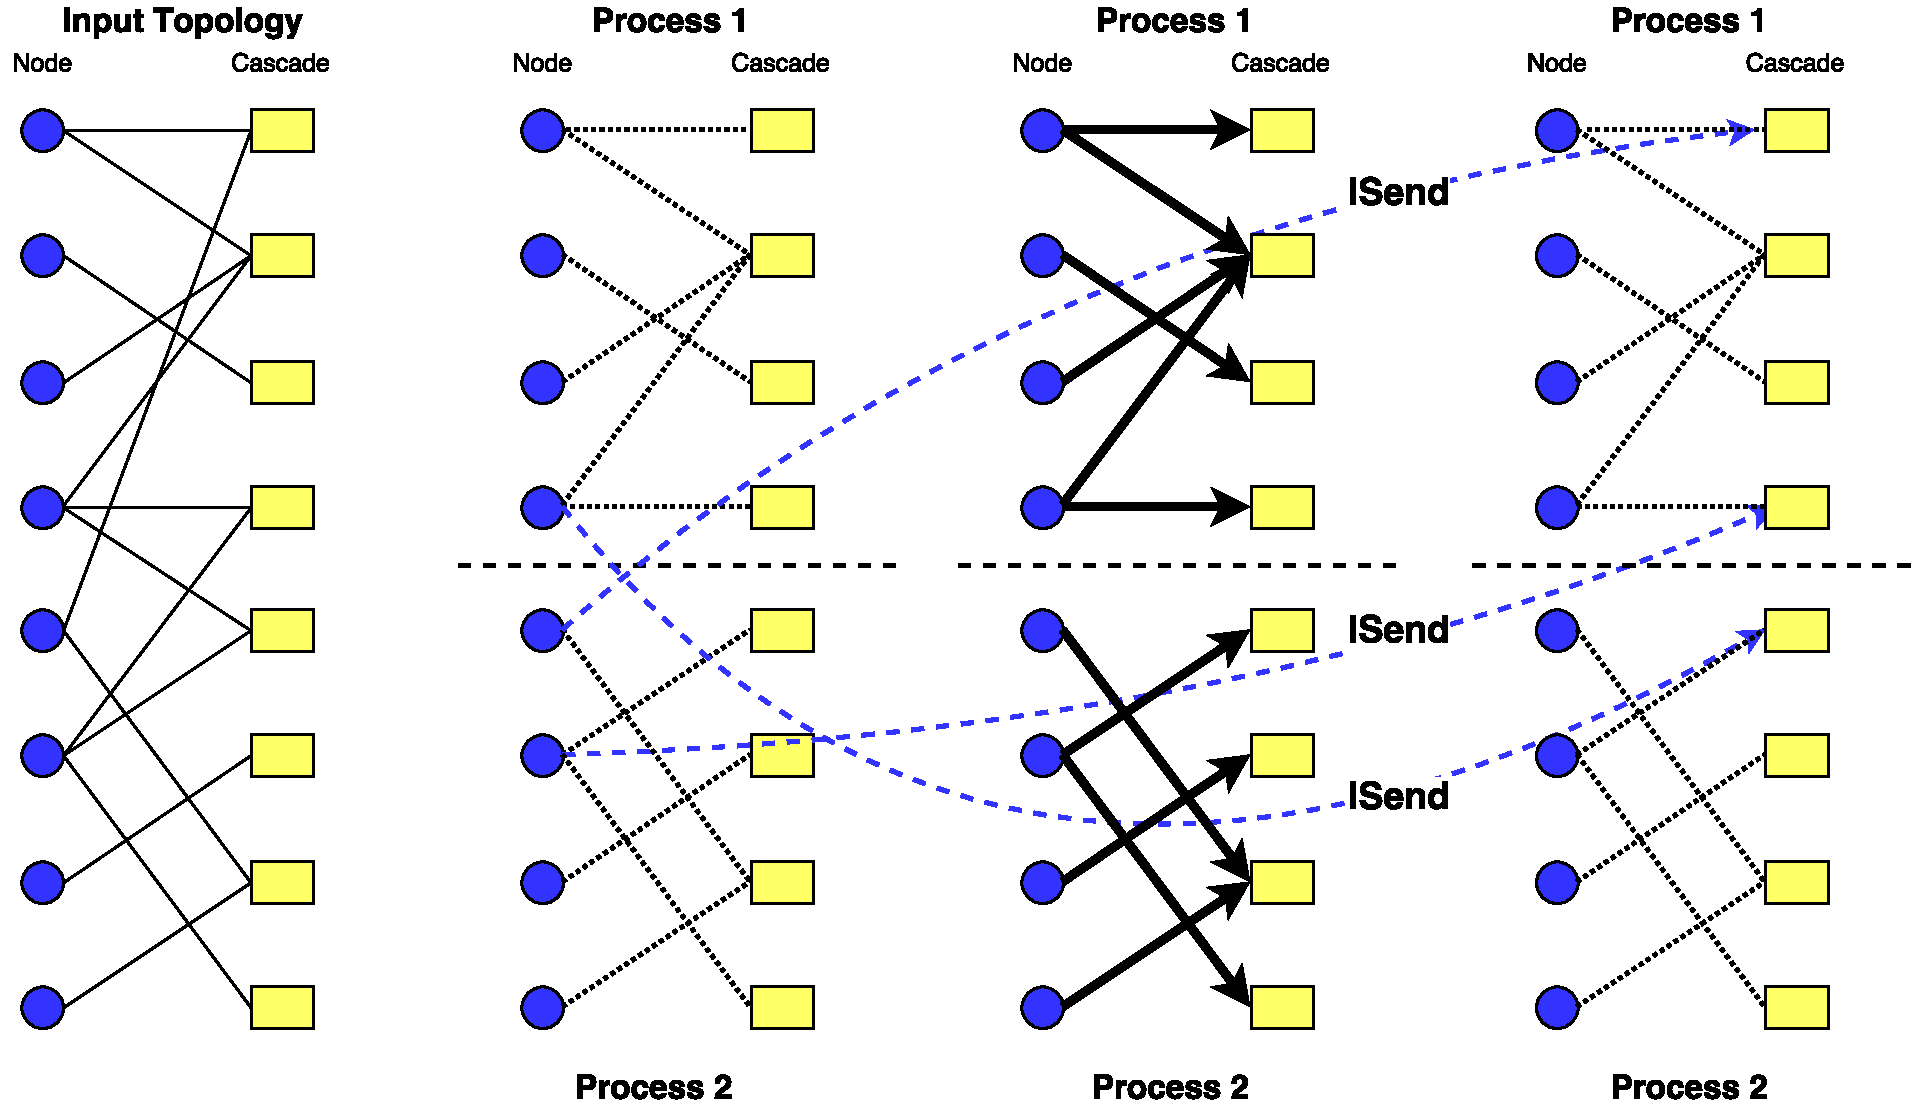
\includegraphics[width=.8\textwidth]{img/chap3/propagation_node_casc.pdf}
\centering
\caption{Illustration of the parallelization scheme using two processors. The parameters propagate back and forth between nodes and cascades iteratively. If the connected node and cascade are in the different processors, the parameters are sent via asynchronous communication, i.e. the blue dashed lines marked by ``ISend''. At the same time, the local parameter propagation occurs within each processor, i.e. the bold black arrows in the middle. This figure illustrates the parameter propagation from node layer to cascade layer. The parameter propagation from cascade layer to node layer is conducted in a similar manner.}\label{fig:pll}
\end{figure}
\begin{algorithm}
\caption{Parallelized SGA Algorithm (Distributed Memory Machines)}\label{algo:2}
\begin{algorithmic}[1]
\For {each cascade $c$}
\State $proc(c) = $ ID of the processor storing $M_c$
\EndFor
\For {each node $u$}
\State $proc(u) = $ ID of the processor storing $A_u$
\EndFor
\ForAll {each processor $p$ {\bf in parallel}}
\State $U_p = $ IDs of the nodes owned by processor $p$
\State $C_p = $ IDs of the cascades owned by processor $p$
\EndFor
\For {each SGA iteration}
\ForAll {each processor $p$ {\bf in parallel}}
\State Call Algorithm~\ref{algo:3} to update $M_c$s using $A_u$s
%\LineComment{Update $A_u$s using $M_c$s}
%\LineComment{Update $A_u$s using $M_c$s}
\EndFor
\ForAll {each processor $p$ {\bf in parallel}}
\State Call Algorithm~\ref{algo:3} to update $A_u$s using $M_c$s similarly
%\LineComment{Update $A_u$s using $M_c$s}
%\LineComment{Update $A_u$s using $M_c$s}
\EndFor
\EndFor
\end{algorithmic}
\end{algorithm}

\begin{algorithm}
\caption{Parallelized SGA Updates of $M_c$s using $A_u$s (Distributed Memory Machines)}\label{algo:3}
\begin{algorithmic}[1]
%\State \COMMENT{\it 1.a Message passing}
\For {each $(u,c)$ s.t. $u \in U_{p}$, $c \notin C_p$ and $u \in V_c \cup D_c$}
\State Send $A_u$ to $proc(c)$ asynchronously
\EndFor
%\State \COMMENT{\it 1.b Local updates}
\For {each $(u,c)$ s.t. $u \in U_{p}$, $c \in C_p$ and $u \in V_c \cup D_c$}
\State Call Algorithm~\ref{algo:sga1} to update $M_c$ using $A_u$.
\EndFor
\State Wait for asynchronous receive requests until done
%\State \COMMENT{\it 1.c Remote updates}
\For {each $(u,c)$ s.t. $u \notin U_{p}$, $c \in C_p$ and $u \in V_c \cup D_c$}
\State Call Algorithm~\ref{algo:sga1} to update $M_c$ using $A_u$.
\EndFor
\end{algorithmic}
\end{algorithm}

Figure~\ref{fig:pll} illustrates this parallelization scheme. The three phases described above are represented by the three diagrams following the first diagram showing the initial stage in Figure~\ref{fig:pll}. The parameters propagate back and forth between node layer and cascade layer iteratively. If the connected node and cascade are in the different processors, the parameters are sent via asynchronous communication, i.e. the blue dashed lines labeled ``ISend''. At the same time, the local parameter propagation occurs within each processor, as indicated by the bold black arrows in the middle. Using the same protocol, we can update $A_u$s using the values of $M_c$s.

After distributing nodes and cascades to the processors, each processor creates its private memory space for the $A_u$s and $M_c$s it owns and ghost memory space for those $A_u$s and $M_c$s connected to the nodes or cascades in the bipartite graph, but owned by other processors. In every SGA iteration, once the ghost memory is filled with the received data, it will not be written again. For example, a processor owns two nodes $u$ and $v$, both involved in a cascade $c$ which is owned by another remote processor. To update $A_u$ and $A_v$, $M_c$ is sent asynchronously to this local processor. But $M_c$ will be sent only once regardless of the number of associated nodes owned by the local processor, because $M_c$ can be shared by the updates of $A_u$ and $A_v$. This optimization is similar to the combiner applied to the message queues in Pregal-like parallel graph processing systems~\cite{malewicz2010pregel,avery2011giraph} to avoid sending duplicated messages to the same target processor.

We test our parallelization scheme on RPI Advanced Multiprocessing Optimized System (AMOS), which is a 5-rack, 5K nodes, 80K cores IBM Blue Gene/Q system~\cite{haring2012ibm} with additional equipment. In AMOS supercomputer, each node consists of a 16-core, 1.6 GHz A2 processor, with 16 GB of DDR3 memory. Considering the fact that the inter-core communication is generally more efficient inside the same node than across different nodes, we use all the 16 cores of a node so that the communication between cores can be more efficient. In general, the maximum number of cores per node here is not constrained by the limit of 16 GB DDR3 memory space. This is one benefit of our memory management paradigm because every processor stores only one copy of the parameters of nodes and cascades associated with it.

\begin{figure}[t]
\centering
\begin{tabular}{c}

\begin{subfigure}{.45\textwidth}
\centering
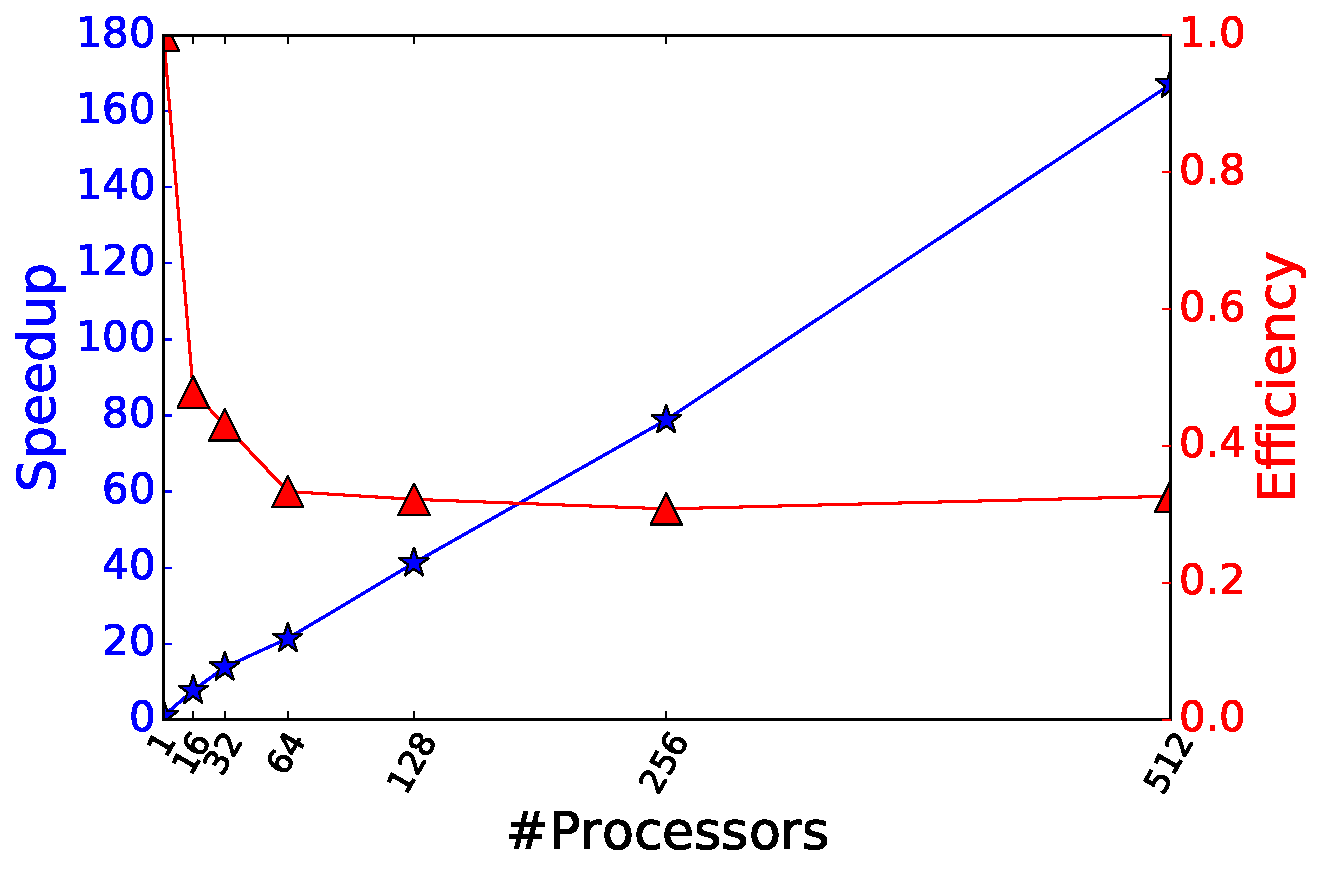
\includegraphics[width=.99\linewidth]{img/chap3/Speedup_SBM_v1_D100.pdf}
\caption{m=100}\label{fig:Speedup_SBM_v1_D100}
\end{subfigure} 
\begin{subfigure}{.45\textwidth}
\centering
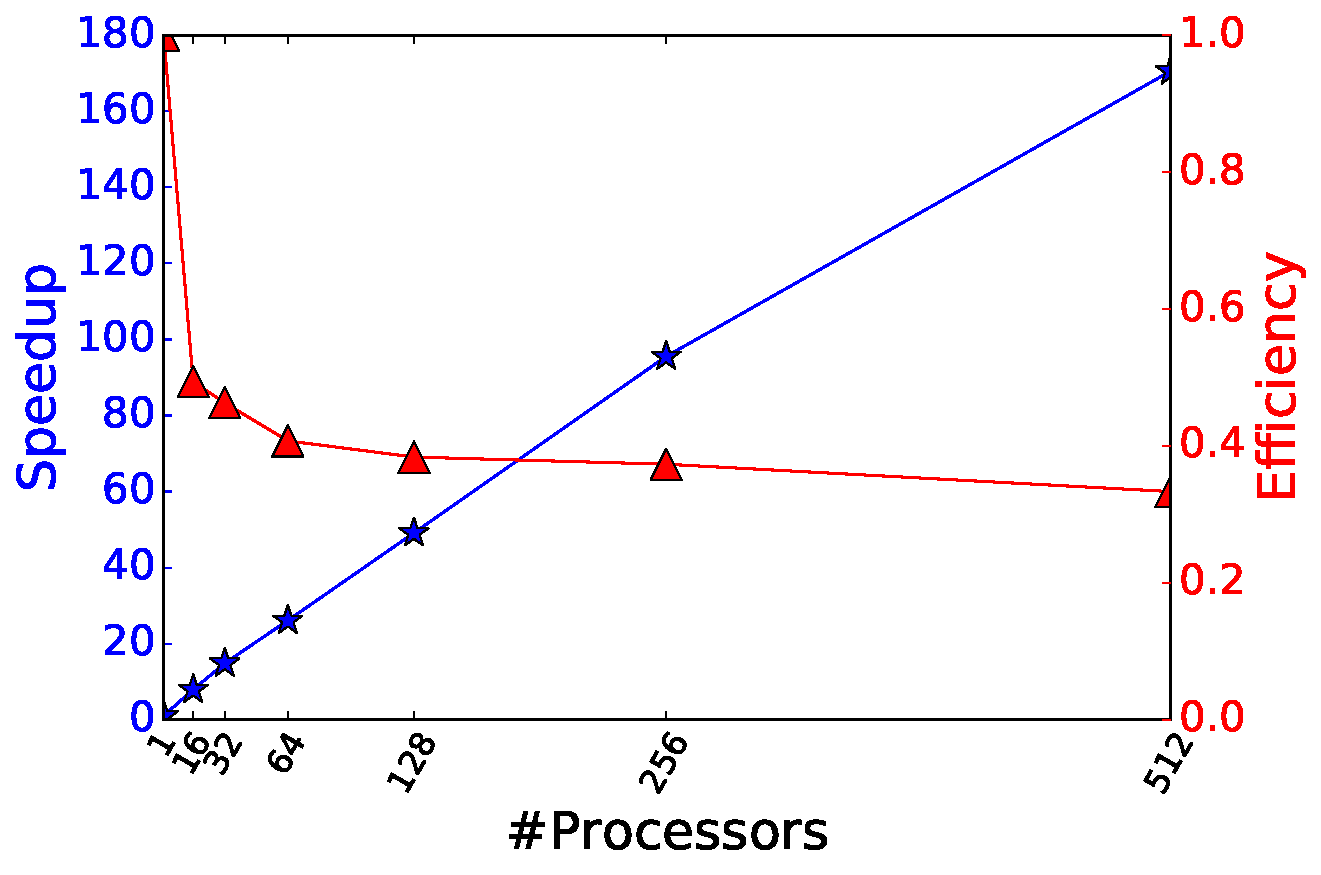
\includegraphics[width=.99\linewidth]{img/chap3/Speedup_SBM_v1_D200.pdf}
\caption{m=200}\label{fig:Speedup_SBM_v1_D200}
\end{subfigure} 

\end{tabular}
\caption{Speedup and efficiency of our parallelization scheme on Advanced Multiprocessing Optimized System (AMOS). $m$ denotes the dimension of $A_u$ and $M_c$.}
\label{fig:speedup_efficiency}
\end{figure}

%SBM_v1.txt 20K nodes, 10K cascades
The speedup and efficiency of our parallelization scheme are shown in Figure~\ref{fig:speedup_efficiency}. A total of 10K cascades are simulated on the SBM network with 20K nodes. Each cascade infects a total of 247 nodes on average. The Figure~\ref{fig:speedup_efficiency} shows that the parallelization scheme achieves an approximately linear speedup using several hundreds of processors. And the efficiency of the parallelization scheme is above 25\% in all cases. The comparison between Figure~\ref{fig:Speedup_SBM_v1_D100} and Figure~\ref{fig:Speedup_SBM_v1_D200} shows that the dimension $m$ does not change the speedup or efficiency. In our sampled GDELT dataset, the parallelized algorithm achieves the similar speedup and efficiency using 64 processors, but adding extra processors does not significantly increase the speedup due to the limited size of the dataset.

To test the scalability of the parallelization scheme, we evaluate the execution time of one single SGA iteration of Algorithm~\ref{algo:2} using 512 processors. Given a network of 10K nodes and the different numbers of cascades, Figure~\ref{fig:node_number_time} shows that the execution time is approximately proportional to the number of cascades. A similar pattern is also observed as the dimension $m$ grows. In contrast, when the number of cascades is fixed and the number of network nodes increases, the execution time grows slowly - the execution time only doubles when the number of network nodes grows from 5K to 20K. The reason is that the number of infections per cascade is relatively stable in the synthetic data so that the increase of time for parameter propagation is actually smaller than the increase in the number of network nodes. In general, the parallelization scheme scales well with the number of network nodes, the number of cascades and the dimension $m$.

\begin{figure}[t]
\centering

\begin{subfigure}{.45\textwidth}
\centering
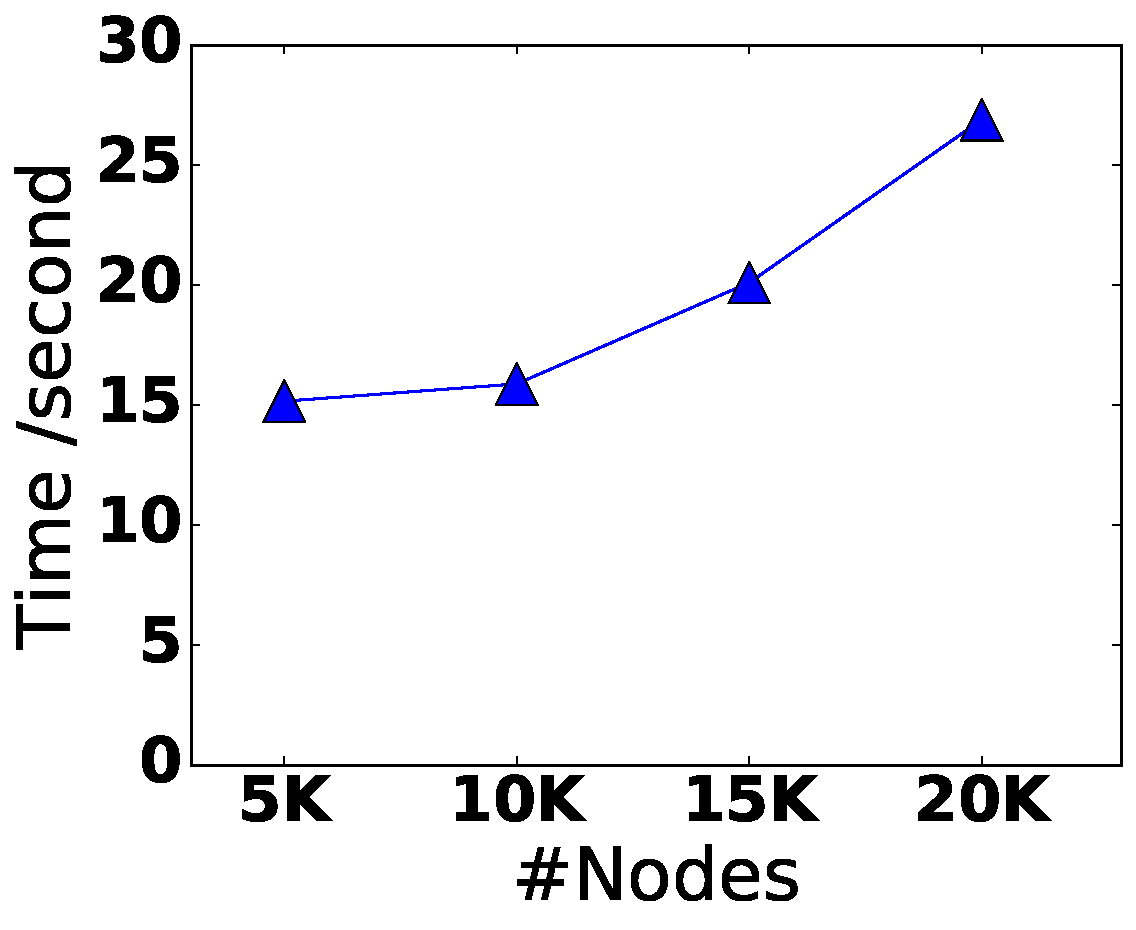
\includegraphics[width=.99\linewidth]{img/chap3/node_number_time.pdf}
\caption{m=200}\label{fig:node_number_time}
\end{subfigure} 
\begin{subfigure}{.45\textwidth}
\centering
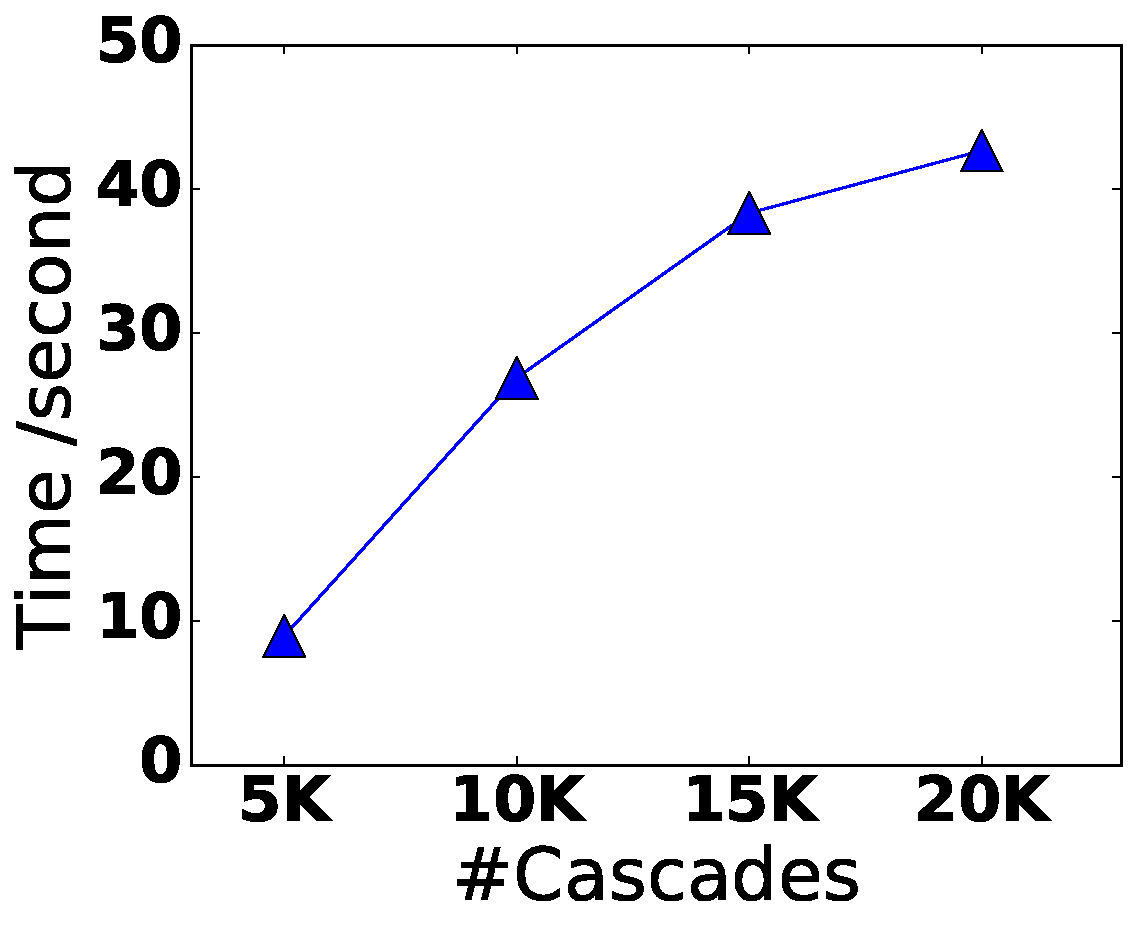
\includegraphics[width=.99\linewidth]{img/chap3/cas_number_time.pdf}
\caption{m=200}\label{fig:cas_number_time}
\end{subfigure} %
\hfill

\begin{subfigure}{.45\textwidth}
\centering
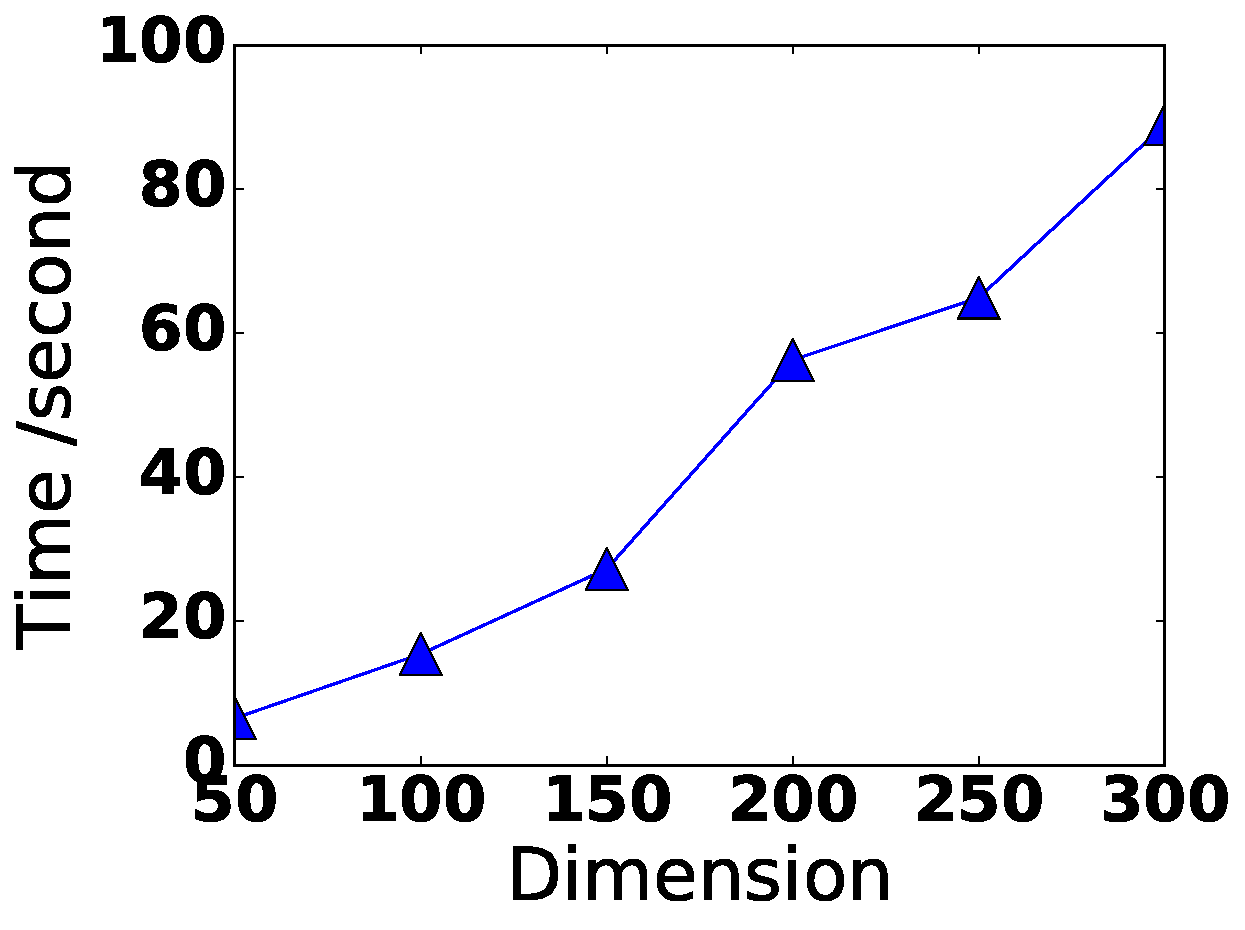
\includegraphics[width=.99\linewidth]{img/chap3/dimension_time.pdf}
\caption{m=200}\label{fig:dimension_time}
\end{subfigure} 

\caption{The execution time of one SGA iteration in relation to the dimension $m$, the number of network nodes and the number of cascades.}
\end{figure}

\begin{table*}[ht]
\caption{Accuracy of the news virality prediction measured by F1 scores. The predictions of our proposed model (ML) are consistently better than the the baseline model's (BL) using the same set of early adopters in the first 30 to 60 minutes.}
\centering
\label{tab:onehour}
\begin{tabular}{|c|c|c|c|c|c|c|c|c|c|c|}
\hline
\multirow{2}{*}{Threshold $\theta$} & \multicolumn{2}{c|}{$\tau=$0.5 Hour} & \multicolumn{2}{c|}{$\tau=$0.6 Hour} & \multicolumn{2}{c|}{$\tau=$0.7 Hour} & \multicolumn{2}{c|}{$\tau=$0.8 Hour} & \multicolumn{2}{c|}{$\tau=$0.9 Hour} \\ \cline{2-11}
& BL & ML & BL & ML & BL & ML & BL & ML & BL & ML \\
\hline 
\hline
90\% &  0.410 & 0.500 & 0.410 & 0.497  & 0.410 & 0.499  & 0.499 & 0.549  & 0.499 & 0.548   \\  
\hline
91\% &  0.412 & 0.484 & 0.405 & 0.486  & 0.405 & 0.480  & 0.484 & 0.534  & 0.490 & 0.536   \\
\hline
92\% &  0.389 & 0.473 & 0.394 & 0.472  & 0.392 & 0.471  & 0.463 & 0.530  & 0.463 & 0.531   \\
\hline
93\% &  0.294 & 0.455 & 0.296 & 0.453  & 0.294 & 0.453  & 0.434 & 0.516  & 0.436 & 0.511   \\
\hline
94\% &  0.207 & 0.433 & 0.209 & 0.433  & 0.213 & 0.436  & 0.393 & 0.489  & 0.393 & 0.491   \\
\hline
95\% &  0.191 & 0.404 & 0.191 & 0.409  & 0.195 & 0.408  & 0.352 & 0.465  & 0.347 & 0.462   \\
\hline
96\% &  0.147 & 0.393 & 0.141 & 0.389  & 0.147 & 0.389  & 0.287 & 0.438  & 0.285 & 0.442   \\
\hline
97\% &  0.114 & 0.360 & 0.116 & 0.366  & 0.113 & 0.361  & 0.233 & 0.402  & 0.232 & 0.407   \\
\hline
98\% &  0.097 & 0.311 & 0.091 & 0.316  & 0.097 & 0.316  & 0.160 & 0.365  & 0.166 & 0.357   \\
\hline
99\% &  0.119 & 0.288 & 0.107 & 0.292  & 0.104 & 0.279  & 0.148 & 0.326  & 0.148 & 0.324   \\
\hline
\end{tabular}
\end{table*}


\subsection{Virality prediction via early adopters} \label{sec:forecast}
Our aim is to forecast the viral information cascade. From the historical cascades, the proposed model estimates the $A_u$ vector for each $u$ according to the observed response times. Using these $A_u$ vectors of the initially infected nodes, we seek to predict the behavior of future cascades.

Suppose a set of so-called early adopters have been infected within a limited time period. One basic observation is that, once the contagion reaches a community member, the probability that other members get infected increases. Therefore, we can make use of the infected node's local neighborhood to predict the infection future. Since our model presents every node $u$ by a vector $A_u$ in the latent space, it is easy to find the neighbors which are close to node $u$ by measuring the Euclidean distances between them. As the contagion is likely to spread fast in the dense areas, the number of neighbors within a certain range can be used as an indicator of future infections. Hence, we count the number of neighbors that are located within a certain range from the infected node $v$, and arrange these values in a vector $K$ whose $i$-th component is defined as
\begin{equation} \label{eq:prediction_}
K_i = |\{u|\|A_u - A_v\|_2 < r_i\}|
\end{equation}
where $r_i$ is the radius of the $i$-th neighborhood of node $v$ and $\|\cdot \|_2$ denotes the Euclidean norm.

Figure~\ref{fig:hood} demonstrates how to compute the $K$ vector of an infected node. Suppose the infected nodes are located at the centers of the different circles. Their neighborhoods are marked by the circles which have the radii $r_1$, $r_2$ and $r_3$ respectively. In Figure~\ref{fig:hood}, the node at the right center has 3 neighbors inside the small circle, 7 neighbors inside the medium circle and 12 neighbors inside large circle, resulting in the vector $K=[3,7,12]$. The leftmost node has only 1 neighbor, i.e. itself, inside both the small and medium circle and 5 neighbors inside the large circle, resulting in the vector $K'=[1,1,5]$. Intuitively, we can tell from $K$ and $K'$ that the right three neighborhoods allow faster growth of infections than the left ones. 

Given a set of early adopters which get infected within a limited time period, we can count the total number of \textbf{unique} neighbors in their local neighborhoods within different radii similarly. Note that if a node is in the $i$-th neighborhood of two early adopters, this node is only counted once in the $i$-th component of $K$. Finally, The numbers of neighbors, presented as the components of a multiple-dimensional vector $K$, are fed to a machine learning model to predict the final size of a cascade.

\begin{figure}
    \centering
    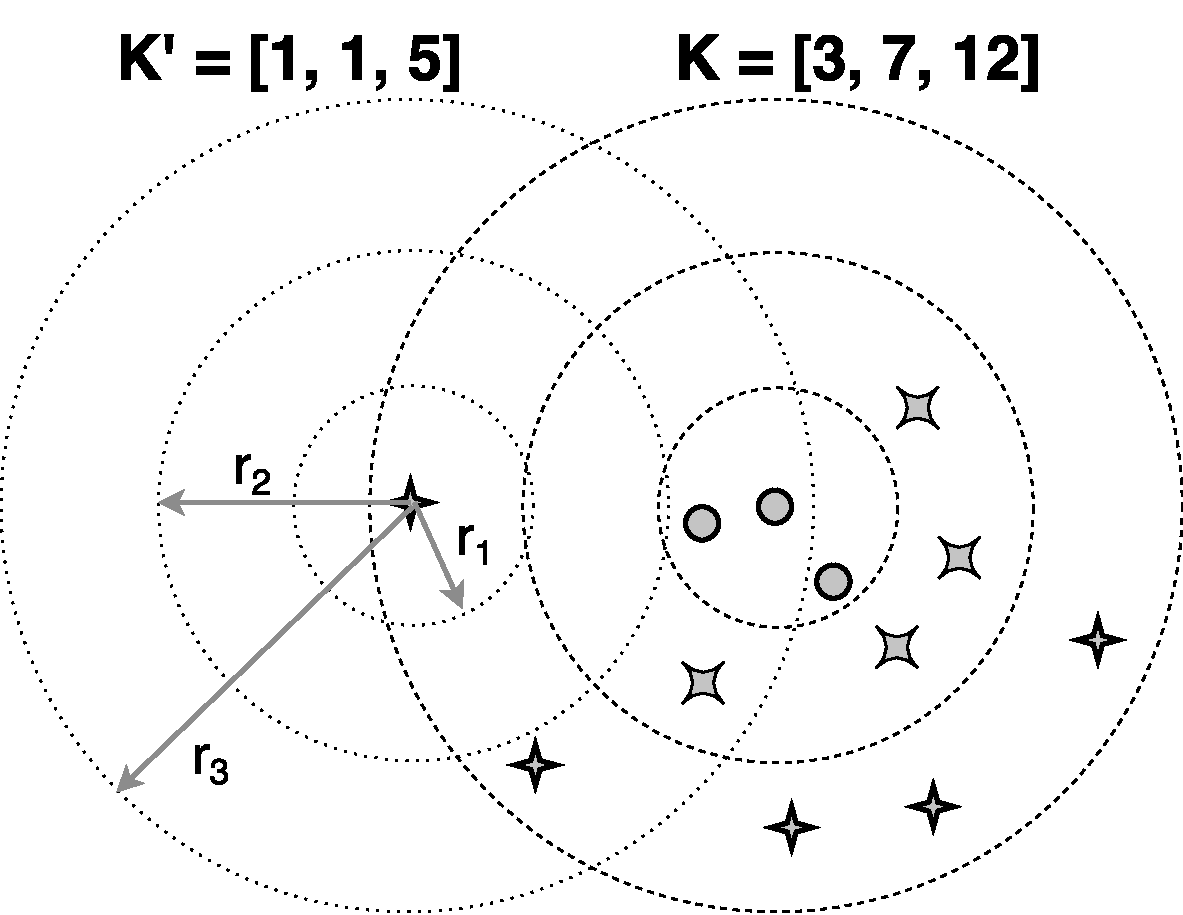
\includegraphics[width=.7\textwidth]{img/chap3/hood.pdf}
    \caption{Illustration of the local neighborhoods in the vector space. The concentric circles mark the neighborhoods with different radii from the center. The proposed method counts the number of nodes located in each circle and arrange these values in a vector. Vector $K$ shows the numbers of nodes for $r_1$, $r_2$ and $r_3$ radii drawn from the figure center while $K'$ is shown for the circles centered at the asterisk on the left.}
    \label{fig:hood}
\end{figure}

Our model produces the $A_u$ vector for each node $u$ in the network. If these $\{A_u\}$ vectors preserve the community structures of the news media network well, their clustering should match the community structure embedded in the explicit network topology, because the members of a community have similar $A_u$s.

Given a synthetic SBM network, we simulate the cascades as described in Section~\ref{sec:3.2.1}. Our model then infers the $\{A_u\}$ vectors by these cascades. For clarity, the set of nodes detected in a network is called a community and the set of nodes clustered by their vector representations is called a cluster here. We compare the node clustering of these $\{A_u\}$ vectors with the ground truth partition of the SBM network and the community structures discovered by traditional community detection algorithms from the explicit topology. The alignment between them indicates the $\{A_u\}$ vectors produced by our model preserve the community structures.

More specifically, the K-means clustering algorithm~\cite{macqueen1967some} is executed on the so-inferred $\{A_u\}$ vectors to derive the node clustering. The similarity between the node clustering and the contrastive partitioning of the network are measured by the Adjusted Mutual Information (AMI) and Adjusted Rand Score (ARS) which are widely used to evaluate community detection performance. Section~\ref{sec:2.2.3} presents the mathematical definitions of both metrics.

\begin{figure}
    \centering
    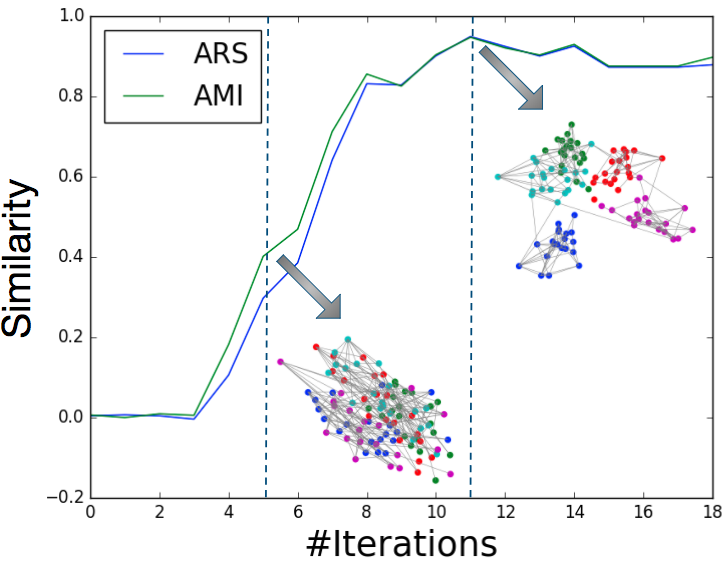
\includegraphics[width=.8\textwidth]{img/chap3/converge.png}
    \caption{The similarity between the node clustering of the $\{A_u\}$ vectors at each SGA iteration of Algorithm~\ref{algo:sga1} and the ground truth partition of the SBM network.}
    \label{fig:alignment_figure}
\end{figure}

\begin{table}[]
\caption{The pairwise similarities between the communities detected by the state-of-the-art community detection algorithms, the node clustering of the $\{A_u\}$ vectors produced by our model and the ground truth partition of the SBM network. The entries below and above the main diagonal represent the Adjusted Rand Score (ARS) and Adjusted Mutual Information (AMI) respectively. FG: Fast Greedy algorithm~\cite{clauset2009power}, LE: leading eigenvector method~\cite{newman2006finding}, LP: label propagation algorithm~\cite{raghavan2007near}, ML: multilevel algorithm~\cite{blondel2008fast}. Our model produces node embeddings whose clustering aligns well with the ground truth communities, even outperforming some community detection baseline methods.}\label{tab:alignment_table}
    \centering
    \begin{tabular}{|c|cccccc|}
   \hline
    ARS / AMI & FG & LE & LP & ML &  Our Model &  Ground Truth\\
   \hline
FG &  & 0.858 & 0.833 & 0.943 & 0.881 & 0.933 \\
LE & 0.873 &  & 0.807 & 0.867 & 0.795 & 0.837 \\
LP & 0.864 & 0.829 &  & 0.835 & 0.773 & 0.804 \\
ML & 0.929 & 0.881 & 0.868 &  & 0.922 & 0.949 \\
Our Model & 0.869 & 0.820 & 0.817 & 0.936 &  & 0.930 \\
Ground Truth & 0.939 & 0.865 & 0.852 & 0.963 & 0.925 & \\
\hline
    \end{tabular}
\end{table}

Figure~\ref{fig:alignment_figure} shows the growth of the similarity between the node clustering of the $\{A_u\}$ vectors at each SGA iteration and the ground truth partition of the SBM network. The SBM network has 100 nodes and 5 communities of size 20, 190 edges connects nodes in the same community and 12 edges are across different communities. A total of 100 cascades are simulated, each involves 12.5 infections on average. The dimension of $A_u$ is $m=10$. After each SGA iteration of Algorithm~\ref{algo:sga1}, we compute a $100\times 100$ distance matrix with the $(u,v)$ entries being the Euclidean distances between the latest updated vectors $A_u$ and $A_v$. The plots for two networks in Figure~\ref{fig:alignment_figure} are made by the MDS algorithm~\cite{cox2000multidimensional} which places each node in two-dimensional space such that the derived between-node distances are preserved as well as possible. In other words, the MDS coordinates preserve the nodes' pairwise distances in the high-dimensional space of $\{A_u\}$. At the 5th iteration, the ARS and AMI scores are around 0.4, the nodes' MDS coordinates do not reflect their ground truth communities represented by the color. When the 11th SGA iteration is done, the ARS and AMI scores become greater than 0.9, and the nodes' MDS coordinates match the community structures very well. Figure~\ref{fig:alignment_figure} shows that, as the inference algorithm proceeds, the $\{A_u\}$ vectors start to preserve the community structures, even though our model takes only the infection delays in the cascades as input, but not the the explicit network topology.


%SBM_10K nodes, 10K cascades, D=200 for Table 1
\begin{table}[ht]
  \centering
  \caption{Quality metric of the detected communities on synthetic SBM networks with 10K nodes. ARS: Adjusted Rand Score; AMI: Adjusted Mutual Information.}
  \begin{tabular}{ccccc}
    \hline
    \#Processors & {\bf 1} & {\bf 4} & {\bf 16} & {\bf 64}\\
    \hline
    ARS & 0.9588 & 0.9480 &	0.9444 & 0.9704\\
    AMI & 0.9858 & 0.9814 & 0.9808 & 0.9888\\
    \hline
  \end{tabular}
  \label{tab:chap3_1}
\end{table}

\begin{figure}[ht!]
\centering

\begin{subfigure}{.45\textwidth}
\centering
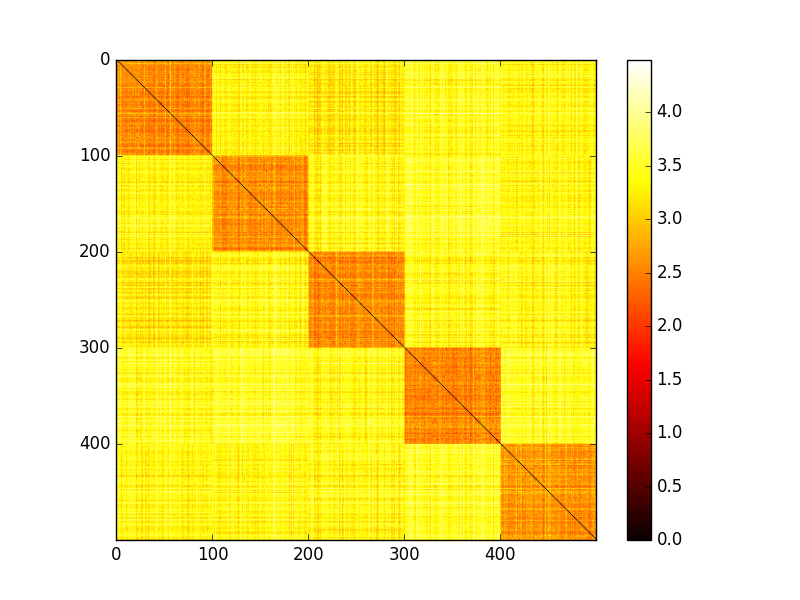
\includegraphics[width=.99\linewidth]{img/chap3/heatmap_P1.png}
\caption{1 processor}\label{fig:c1}
\end{subfigure} 
\begin{subfigure}{.45\textwidth}
\centering
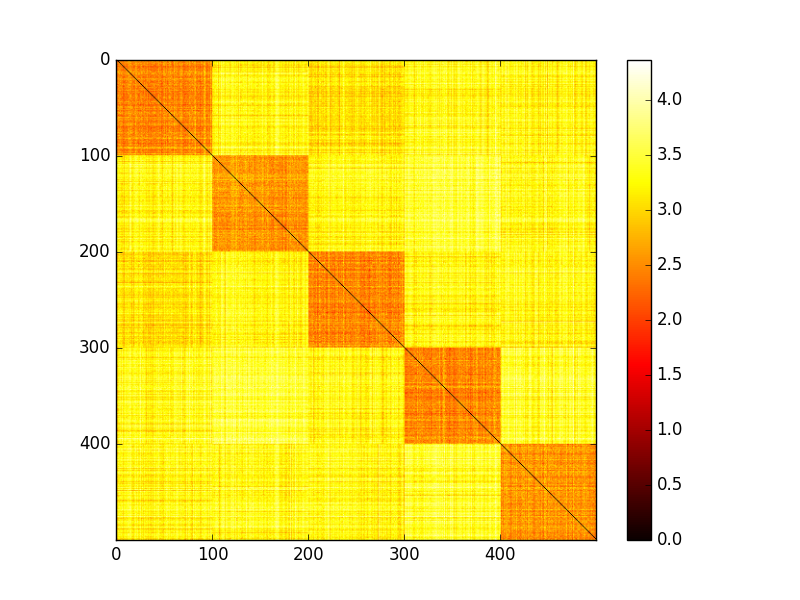
\includegraphics[width=.99\linewidth]{img/chap3/heatmap_P4.png}
\caption{4 processor}\label{fig:c2}
\end{subfigure} %
\hfill
\begin{subfigure}{.45\textwidth}
\centering
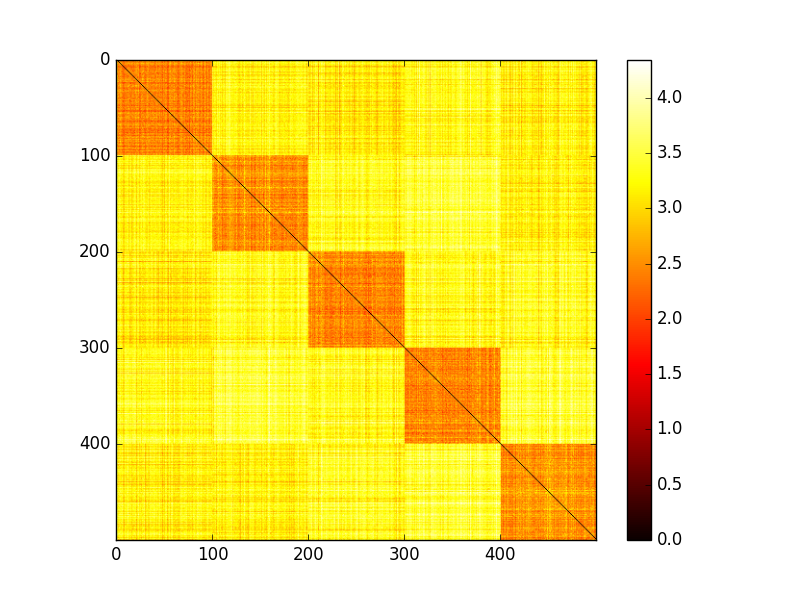
\includegraphics[width=.99\linewidth]{img/chap3/heatmap_P16.png}
\caption{16 processor}\label{fig:c3}
\end{subfigure} 
\begin{subfigure}{.45\textwidth}
\centering
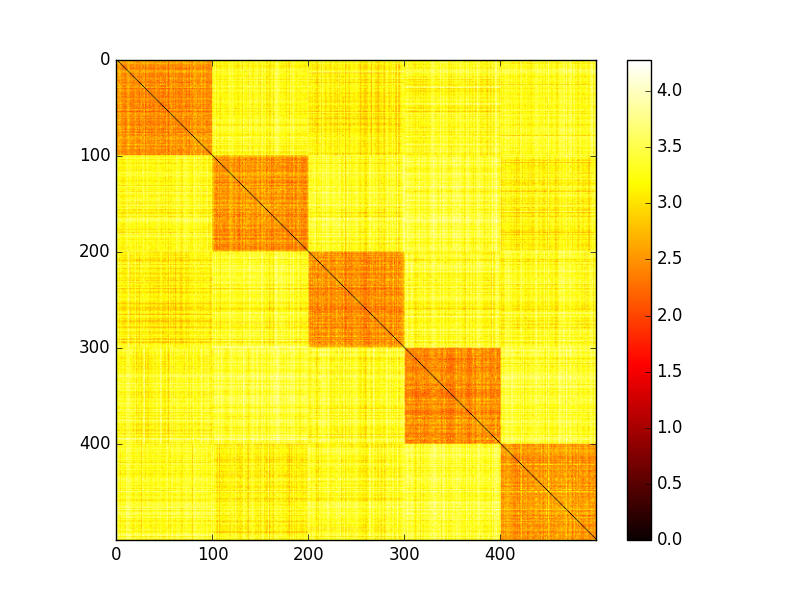
\includegraphics[width=.99\linewidth]{img/chap3/heatmap_P64.png}
\caption{64 processor}\label{fig:c4}
\end{subfigure} 

\caption{Distance matrix of the first 500 nodes of synthetic SBM networks based on the node embeddings produced by different number of processors. The color in the distance matrix indicates the distance between a pair of nodes, brighter the color longer the distance.}
\label{fig:tab1_fig}
\end{figure}

In addition, we compare the node clustering of $\{A_u\}$ vectors at the 15th iteration with the ground truth partition of the SBM network and community structures detected by the state-of-the-art algorithms such as Fast Greedy algorithm~\cite{clauset2009power}, leading eigenvector method~\cite{newman2006finding}, label propagation algorithm~\cite{raghavan2007near} and multilevel algorithm~\cite{blondel2008fast}. Table~\ref{tab:alignment_table} shows that the alignments between them are good, and that the node clustering of $\{A_u\}$ vectors are more similar to the ground truth partition than the community structures detected by some state-of-the-art community detection algorithms. In Table~\ref{tab:alignment_table}, each entry indicates the similarity of the communities produced by a particular pair of methods. All the entries below the main diagonal correspond to the ARS scores and entries above correspond to the AMI scores. As the ARS and AMI scores indicate, our model produces meaningful node embeddings because the clustering of these node vectors aligns well with the ground truth communities. The community structure obtained by clustering node vectors is even closer to the ground truth than are the community structures detected by the baseline methods that include leading eigenvector method (LE) and label propagation algorithm (LP) are. Our model produces node embeddings whose clustering aligns well with the ground truth communities, outperforming some community detection baselines. In addition, our model does not use the topology of the SBM network like the baseline algorithms do, instead it only accesses the cascades data, which explains why Fast Greedy algorithm (FG) and multilevel algorithm (ML) performs better than our model in terms of community detection. Finally, it should be noted that we choose the number of clusters as 5 for the K-means algorithm here. However this number should be actually systematically selected. We leave the selection of the proper number of clusters for future work.

We also test our algorithm for large SBM networks with the dimension of resulting $A_u$ being 200. In these experiments, there are 100 predefined communities in the SBM network, each containing 100 nodes. Every node is connected to 8.8 nodes in the same community and 1.2 nodes in the other communities on average. And we simulate 10K cascades using the continuous time IC model. As shown in Table~\ref{tab:chap3_1}, as the number of processors increases, the AMI and ARS metrics are consistently above 0.98 and 0.94 respectively, which indicates the resulting $\{A_u\}$ preserves the community structure in the network. The distance matrices of the first 500 nodes are also shown in Fig.~\ref{fig:tab1_fig}. In the distance matrix, the distance between two nodes $u$ and $v$ is defined as the Euclidean distance between vectors $A_u$ and $A_v$ and this value is visualized by the color brightness in the heatmap, brighter the color longer the distance. Each dense module in this matrix comprises 100 nodes and matches the predefined SBM community very well. As illustrated by the visualized pair-wise nodes distance matrices, the number of processors does not change the high quality of $\{A_u\}$ as the resulting vectors preserve the community structure of SBM networks in all cases. Our model does not use the topology of the SBM network, instead it only accesses the response times of the nodes to different cascades, yet the community structure can still be accurately recovered from these response times.

Our aim is to predict the viral news cascades at their early stage. Specifically, with the global news dataset of events, the task is to predict the most reported events within a limited time period. Therefore, we rank the events reported in the news by the number of their reports and divide them into two classes: those who are among the top $(1-\theta)$ percent of this ranking and the remaining events. In this way, we can treat the virality prediction as a binary classification problem - given the early reports within a limited time period, can we classify the events reported in the news into these two categories? Since we are only interested in predicting the most viral events reported in the news, the threshold $\theta$ ranges from 90\% to 99\% in our experiments. Notice that a high threshold $\theta$ would result in two very imbalanced sets of samples, which would make the prediction challenging.

\textbf{Baseline} We build a baseline algorithm which uses multiple features extracted from cascade early progress and the Random Forest model~\cite{liaw2002classification} for cascade classification. We choose Random Forest for comparison because, as an ensemble learning method, it is known to work well with the non-linear growth of modeled phenomena such as the viral spread of news reports. The extracted features include the number of unique early adopters, the frequency of the infections at the early stage, the maximum interval between two continuous infections, and the minimum interval between two continuous infections. In contrast, our proposed model uses the numbers of neighbors in different ranges from the infected nodes, i.e. vector $K$ presented in Eq.~\ref{eq:prediction_}, as the input of the Random Forest model. For a fair comparison, both the baseline and our model use the information about the early adopters in the first $\tau$ hours, where $\tau$ ranges from $0.5$ to $3$.

\begin{figure}
    \centering
    \hspace*{-1.5cm} 
    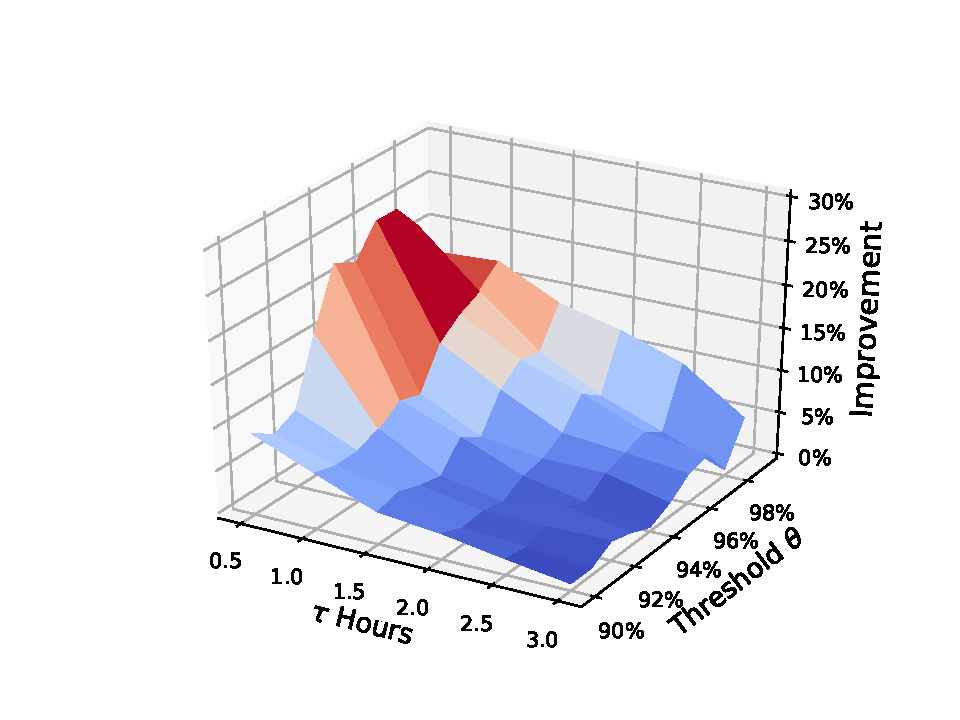
\includegraphics[width=8cm]{img/chap3/improvement3d.pdf}
    \caption{The improvement in virality prediction accuracy produced by our model in GDELT dataset in relation to the classification threshold $\theta$ and the initial observation period of $\tau$ hours.}
    \label{fig:improvement3d}
\end{figure}

The accuracy of the prediction is evaluated by the F1 score which is commonly used in the classification problems

\begin{figure*}[t]
\centering

\begin{subfigure}{.32\textwidth}
\centering
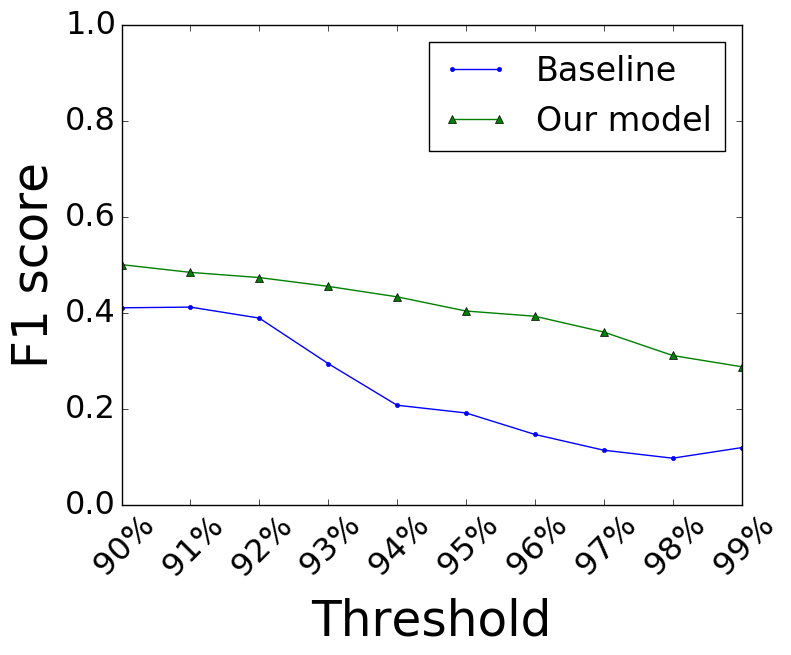
\includegraphics[width=.99\linewidth]{img/chap3/gdelt_30_mins.png}
\caption{$\tau=0.5$ hours}\label{fig:gdelt1}
\end{subfigure}
\begin{subfigure}{.32\textwidth}
\centering
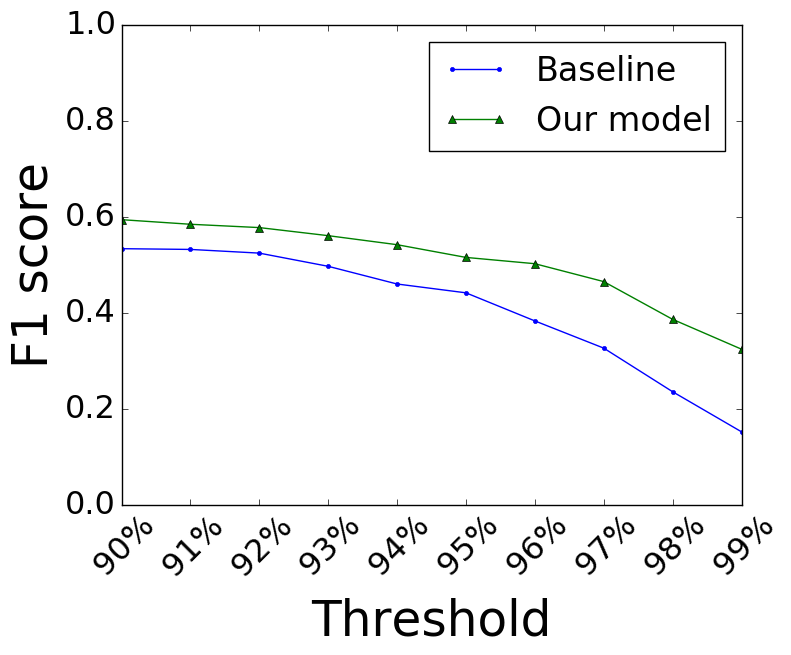
\includegraphics[width=.99\linewidth]{img/chap3/gdelt_60_mins.png}
\caption{$\tau=1$ hours}\label{fig:gdelt2}
\end{subfigure}
\begin{subfigure}{.32\textwidth}
\centering
\includegraphics[width=.99\linewidth]{img/chap3/gdelt_90_mins.png}
\caption{$\tau=1.5$ hours}\label{fig:gdelt3}
\end{subfigure} %
\hfill
\begin{subfigure}{.32\textwidth}
\centering
\includegraphics[width=.99\linewidth]{img/chap3/gdelt_120_mins.png}
\caption{$\tau=2$ hours}\label{fig:gdelt4}
\end{subfigure}
\begin{subfigure}{.32\textwidth}
\centering
\includegraphics[width=.99\linewidth]{img/chap3/gdelt_150_mins.png}
\caption{$\tau=2.5$ hours}\label{fig:gdelt5}
\end{subfigure}
\begin{subfigure}{.32\textwidth}
\centering
\includegraphics[width=.99\linewidth]{img/chap3/gdelt_180_mins.png}
\caption{$\tau=3$ hours}\label{fig:gdelt6}
\end{subfigure}

\caption{The accuracy of virality prediction in global news dataset of events (i.e. GDELT) measured by the F1 score. The prediction models take the news sites reporting an event in the first $\tau$ hours, i.e. the early adopters, as input.}
\label{fig:gdelt_prediction}
\end{figure*}

\begin{equation}
F_1 = \frac{2 \cdot \text{\it precision}\cdot \text{\it recall}}{\text{\it precision}+\text{\it recall}}
\end{equation}
F1 score considers both the precision and recall of virality prediction. A decent F1 score prevents the system from either predicting too many viral news with a high false positive rate, or from being too conservative making insufficient predictions.

Figure~\ref{fig:gdelt_prediction} shows the F1 scores of the 6-fold cross validation tests using a variety of $\tau$ values. As the threshold $\theta$ increases, the F1 scores of both the baseline and our model decrease due to the imbalanced sets of samples. The F1 scores of the prediction made by our model are consistently better than the baseline's. Specifically, our model outperforms the baseline by 10\% in most cases. As shown in Figure~\ref{fig:improvement3d}, the improvement produced by our model is very obvious when the value of $\tau$ becomes small. It is because our model uses the community structure of the propagation network which is not included in the feature-based baseline model. As the value of $\tau$ increases, both the baseline model and our proposed model gain better performance, yet the performance gap between them decreases at the same time. One potential reason is that the information cascades start to slow down inside each communities at this stage with $\tau>2$. Thus, the community structure does not provide extra signal for the prediction as it does at the early stage with $\tau<1.5$. In general, in terms of the prediction accuracy, the influence of $\tau$ value is more significant in the baseline model than in our model, which indicates that community structures can provide the critical signals to forecast the viral information cascades at the early stage.

The relationship between the improvement on prediction accuracy and the classification threshold $\theta$ is shown in Figure~\ref{fig:improvement3d}. Our proposed model performs much better than the baseline model when the threshold is high, and it achieves an almost $25\%$ improvement with the threshold $\theta=98\%$. As discussed in Section~\ref{sec:forecast}, our proposed method calculates the number of neighbors in the early adopters' the local neighborhood, i.e. the number of nodes whose $A_u$ vectors are close to the early adopters' in the latent space. Here, the most plausible explanation is that the most viral cascades have the early adopters in multiple dense areas so that they have advantages in disseminating the contagion to their neighbors in these regions in parallel, resulting in the viral infections within a limited time period. This explanation matches our observation about the viral news in online media - most news about events rarely cross the geographical and cultural boundaries, but once they do, the breaking news draw attention from the news media sites in different regions and hit the headlines very quickly.

\section{Scale-free peer-to-peer network construction} \label{sec:3.3}
The scale-free property is shown to exist in many natural or artificial complex systems, such as protein-protein interaction networks\cite{jeong2001lethality}, the Internet\cite{faloutsos1999power}, the World Wide Web\cite{barabasi1999diameter}, and scientific collaboration networks\cite{barabasi2002evolution}. The degree distribution in these networks follows the power-law: $P(i) \sim  i^{-\gamma}$, where $P(i)$ is the fraction of nodes with degree $i$ and $\gamma$ is the scaling parameter which varies between different types of networks ($2 \leq \gamma \leq 3$ in most cases). In a limited scale-free topology, only nodes with degrees smaller than the hard cut-off (i.e. the maximum) degree have degree distribution that follows the power-law.

The scale-free topology has some good properties, including high tolerance to random attacks\cite{albert2000error}, high synchronizability\cite{korniss2007synchronization} and resistance to congestion\cite{toroczkai2004network}. For this reason, several growth models are proposed to construct the scale-free overlay topology. The BA model\cite{barabasi1999emergence} manages to explain the evolution of scale-free topologies by a core principle named ``Preferential Attachment''. But it is not practical in real distributed applications because the global information is required to maintain it. To address this issue, HAPA\cite{guclu2009limited}, Gaian\cite{bent2008dynamic} and SRA\cite{bulut2014constructing} algorithms were introduced to construct the scale-free overlay topology with partial or no global information.

``Preferential Attachment"\cite{barabasi1999emergence} means a new node is more likely to connect to heavily linked nodes when it joins the network. The BA model has some disadvantages as the growth model for the overlay topology. Firstly, it does not provide hard cut-offs. Since a heavily linked node uses a lot of bandwidth, nodes usually are not willing to maintain high degrees. For this reason, a user-defined hard cut-off (i.e. the maximum) degree is imposed lower than the natural cut-off arising in the BA model. The imposed hard cut-offs restrict the feasible overlays to the limited scale-free topologies, which are more practical. Moreover, the BA model also requires the global information about the topology to add connections when a new node joins. In real-world applications, however, the communication cost of obtaining the global information is prohibitive. Therefore, a distributed approach that constructs the topology without global information is desired.

More formally, the degree of a node is defined as the number of connections it has in an overlay topology. Using the same notation as in \cite{bulut2014constructing}, the fraction of nodes with degree $i$ is denoted as $P_i$,
\begin{equation}
P_i = \frac{N_i}{N}
\end{equation}
where $N_i$ is the number of nodes with degree $i$ and $N$ is the total number of nodes. 

In a scale-free topology, degree distribution follows the power-law: $P_i \sim i^{-\gamma}$ where $\gamma$ is a constant. In a limited scale-free topology, $P_i$ follows the power-law for $i<m$, where $m$ is the hard cut-off (i.e. the maximum) degree.

The value of $P_i$ in a limited scale-free topology is given by Eq. 7 in \cite{bulut2014constructing} as $f_i$ as a function of the maximum degree $m$, the minimum degree $k$ and the scaling parameter $\gamma$, 
\begin{equation} \label{eq:fi1}
f_i = \frac{m - 2 k}{ i^\gamma \sum_{j=k}^{m-1} \frac{m-j}{j^\gamma}}  \quad \text{for} \quad i < m
\end{equation}
and $f_m$, that does not need to follow the power-law distribution, is given as,
\begin{equation} \label{eq:fi2}
f_m = 1 - \sum_{i=k}^{m-1} f_i
\end{equation}
The goal is to maintain the degree distribution as $f_i$ for $i=k,\ldots,m$ while nodes with arbitrary degrees are added or removed. For the sake of simplicity, we assume one node is removed at a time and the node to be removed is denoted as node $R$ and the number of its neighbors is denoted by $b$.

\subsection{Protocol design for dynamic topology construction} 
In \cite{guclu2009limited}, authors propose Hop-and-Attempt Preferential Attachment (HAPA) algorithm\cite{guclu2009limited} where a new node joining the network connects to $k$ (i.e. the minimum degree) nodes in a random route. This scheme works because high degree nodes are more likely to occur in a random route than nodes with low degree. In Gaian algorithm \cite{bent2008dynamic}, a new node broadcasts a message when it joins the network using computing with time principle\cite{szymanski2008computing}. Each receiver computes the maximum time of delay, $t_v$, which is proportional to the inverse of its degree, and chooses the time of delay $t_d$ in the interval $[0, t_v]$ uniformly randomly. Instead of replying to the sender instantly, the receiver waits the time of delay $t_d$ and then replies. In this way, nodes with higher degrees are likely to wait shorter period. The new node connects to the first $k$ responders. It gives a better chance to the new node to connect to nodes with high degrees. This mechanism, which reduces the communication overhead by allowing nodes to self-select themselves according to their fitness to the desired property, is also known as computing with time\cite{szymanski2008computing}. The communication cost for selection is constant in the number of candidates. Similar to HAPA algorithm, Gaian algorithm cannot produce an overlay topology with the user-defined scaling parameter. In addition, post-construction parameters of network structures (i.e. the scaling parameter related to the search performance) cannot be adjusted in these approaches. In \cite{bulut2014constructing}, the authors propose a flexible growth model that can produce a limited scale-free topology with user-defined parameters. The \textbf{S}emi-\textbf{R}andomized Growth \textbf{A}lgorithm (SRA)\cite{bulut2014constructing} requires no global information and imposes a hard cut-off on degrees. In SRA, when a node joins the network, it broadcasts a message containing the desired degrees of the $k$ new neighbors. These degrees are computed according to the given network parameters. The receivers with the desired degrees reply to the new node using computing with time rule \cite{szymanski2008computing}. The new node connects to the first $k$ responders. The scaling parameter, as well as the hard cut-off, can be defined by users in advance. So, the SRA model is able to produce overlay topologies, over which the efficiency of applications such as search algorithms is maximized. The constraints of feasible values of these network parameters are presented in \cite{szymanski2011growing}. SRA outperforms other growth models by producing overlay topologies with perfect matching to the arbitrary power-law degree distribution.

To the best of our knowledge, however, allowing nodes to leave network during overlay maintenance has not been studied. Yet, in peer-to-peer (P2P) networks, nodes are likely to join and leave the network frequently. With such dynamic peer participation, the scale-free topology produced by previous growth models are affected by node removal, especially when hubs are removed. This effect can accumulate, negatively impacting the performance of the P2P network, which are built on top of the overlays. We propose a robust model, in which nodes are allowed to leave the network in an arbitrary pattern. Combined with the growth model proposed in our previous work \cite{bulut2014constructing}, the scale-free topology is maintained while nodes are allowed to freely join and leave the network. We present our approach in detail below.

We propose the following two types of atomic operations that can be conducted by each neighbor of $R$, which is the single node removed from the network:
\begin{itemize}
    \item PUSH: The neighbor of $R$ connects to a new node $A$.
    \item SHUFFLE: Besides connecting to a new node, the neighbor of $R$ also asks the new node $A$ to terminate one connection to some node $B$.
\end{itemize}

We are interested in the degree of every PUSH and SHUFFLE when a single node is removed. Let $D_i$ denote the number of SHUFFLEs on degree $i$ and $I_i$ denote the number of PUSHes on degree $i$. Since $(b-k)$ PUSHes and $k$ SHUFFLEs are needed, we have,
\begin{equation}\label{eq:sumIsumD}
   \begin{array}{rl}
 \sum_{i=k}^{m-1} I_i & = b-k \\
 \sum_{i=k+1}^{m} D_i &= k\\
\end{array} 
\end{equation}

These SHUFFLEs and PUSHs make $D_i$ nodes \textit{decreasing} their degree from $i$ to $(i-1)$ and $I_i$ nodes \textit{increasing} their degree from $i$ to $(i+1)$. Also, $I_m = 0$, $D_k = 0$ because the degrees of all nodes are kept in range $[k, m]$. $I_i$, $D_i$ are non-negative for $i\in[k,m]$.

Consider the total number of nodes with degree $k$ after node $R$ is removed from a network of size $n$. Before removal, there were $(f_k \cdot n)$ nodes originally of degree $k$. Additional $D_{k+1}$ nodes originally with degree $(k+1)$ are added and $I_{k}$ nodes are moved from this count by SHUFFLEs and PUSHes. If the fraction of nodes with degree $k$ is still $f_k$, we have,
\begin{equation} \label{eq:0}
f_k (n-1) = f_k n - I_k + D_{k+1} 
\end{equation}
where $n$ is the total number of nodes before $R$ quits. Similarly, the degrees of $I_{d}$ nodes increase from $d$ to $(d+1)$. The degrees of $I_{d-1}$ nodes increase from $(d-1)$ to $d$. The degrees of $D_{d+1}$ nodes decrease from $(d+1)$ to $d$. And the degrees of $D_d$ nodes decrease from $d$ to $(d-1)$. If the fraction of nodes with degree $d$ remains $f_d$, then
\begin{equation} \label{eq:1}
 f_d (n-1) = f_d n - I_d + I_{d-1} + D_{d+1} - D_d 
\end{equation}
for $k < d < m$ and $d \neq b$. Since node $R$ itself is removed,
\begin{equation} \label{eq:2}
f_b (n-1) = f_b n - I_d + I_{d-1} + D_{d+1} - D_d - 1 
\end{equation}
Due to the hard cut-off, nodes with degree $m$ should not accept any new connections,
\begin{equation} \label{eq:3}
f_m (n-1) = f_m n + I_{m-1} - D_m 
\end{equation}
Simplifying Eqs \ref{eq:0}, \ref{eq:1}, \ref{eq:2}, \ref{eq:3}, we obtain that for $k \leq i \leq b-1$,
\begin{equation} \label{eq:12}
I_{i} - D_{i+1} = \sum_{j=k}^{i} f_j
\end{equation}
and for $  b \leq i < m$,
\begin{equation} \label{eq:13}
I_{i} - D_{i+1} = \sum_{j=k}^{i} f_j - 1
\end{equation}
Let non-negative vectors $\vec{D} = (D_{k+1}, D_{k+2}, \ldots, D_{m})^T$, and $\vec{I} = (I_{k}, I_{k}, \ldots, I_{m-1})^T$ be such that,
\begin{align} \label{eq:vec}
    \vec{I} - \vec{D} &= \begin{bmatrix}
           f_k \\
           f_k+f_{k+1} \\
           \vdots \\
           \sum_{i=k}^{b-1} f_i \\
           \sum_{i=k}^{b} f_i - 1 \\
           \vdots \\
           \sum_{i=k}^{m-1} f_i - 1 \\
         \end{bmatrix}
\end{align}
with the $L^1$ norm $\|\vec{I}\|_1 = b - k$, $\| \vec{D} \|_1 = k$. The solution to Eq. \ref{eq:vec} depends on the degree distribution $f_i$, the degree of removed node $b$ and the hard cut-off $m$, but is independent from the current network size $n$. It allows us to design an algorithm that does not need any global information.\\
One simple solution to Eq. \ref{eq:vec} is,
\begin{align} \label{eq:sol1}
I_i^* &=  \begin{cases}
1 &\text{$ k \leq i < b$}\\
0 &\text{otherwise}
\end{cases}
\end{align}
and for $i \in [k+1, m]$,
\begin{equation} \label{eq:Di_sol}
D_i^* = 1 - \sum_{j=k}^{i-1} f_j
\end{equation}
It could be observed that $D_{i+1}^* = a(i)$ which is the average number of nodes increasing degree from $i$ to $(i+1)$ when a node joins the network in the growth model \cite{bulut2014constructing}. This is because, intuitively, the decreasing degree is exactly the opposite to a new node's connecting to $k$ neighbors.

According to the analysis above, there should be $I_i$ neighbors of $R$ that PUSH on degree $i$ and $D_i$ neighbors of $R$ that SHUFFLE on degree $i$, for $i=k,\ldots,m$. For the specific protocol design, we use the solution $I_i^*$ and $D_i^*$ presented in Eqs \ref{eq:sol1} and \ref{eq:Di_sol}.

Before node $R$ voluntarily quits, it can compute $I_i^*$ and $D_i^*$ locally and assign either the PUSH operation or the SHUFFLE operation to each of its neighbors. The neighbors will PUSH or SHUFFLE as assigned by $R$ before it quits.

If node $R$ crashes due to errors or attacks, it can assign its neighbors the associated operations before the failure. Since the value of $I_i^*$ depends on the degree of $R$, $R$ should re-compute $I_i^*$ and assign the new PUSH/SHUFFLE operations to the neighbors if its degree changes. So, every node whose degree changed sends \textit{updates messages} with its new degree and PUSH and SHUFFLE operations to its neighbors.

If the degree of a node $R$ changes to be $b'$, $R$ computes two non-decreasing sequences,
\begin{equation} \label{eq:uandv}
    v_i = \sum_{j=k+1}^{i} \frac{D_j^*}{k} \quad \textrm{and} \quad
    u_i = \sum_{j=k}^{i} \frac{I_j^*}{b'-k}
\end{equation}
and generates two random values $r_1, r_2$ distributed uniformly over the range $[0, 1)$ for each of the $b'$ neighbors. If $r_1 < k/b' $ and $r_2$ is in the interval $[v_i, v_{i+1})$, then the neighbor SHUFFLEs on degree $i$; if $r_1 \geq k/b' $ and $r_2$ is in the interval $[u_i, u_{i+1})$, then the neighbor PUSHes on degree $i$. In this way, the probability of PUSH on degree $i$ is $(1-\frac{k}{b'}) \frac{I_i^*}{b'-k} = \frac{I_i^*}{b'}$ and the probability of SHUFFLE on degree $i$ is $ \frac{k}{b'} \frac{D_i^*}{k} = \frac{D_i^*}{b'}$.

Furthermore, node $R$ sends the list of its neighbors' IPs in the \textit{update message}. When $R$ is removed from the network, all neighbors of $R$ broadcast the last \textit{update message} sent by $R$. Any receiver with one of the desired degrees in the \textit{update message} connects to the corresponding neighbor of $R$. And each neighbor of $R$ connects only to the first responder. It is worth noting that only one broadcast is needed because all neighbors of $R$ broadcast an identical message and nodes in the network forward the first message they receive.

Applying the solution from Eqs. \ref{eq:sol1} and \ref{eq:Di_sol} to our protocol, we obtain a new Enhanced Semi-Randomized Growth Algorithm (E-SRA): 
\\

\textit{Approach: E-SRA (Assuming one node is removed at a time)} To remove a node $R$ with degree $b$, each neighbor of $R$ either SHUFFLEs on degree $i$ by the probability $\frac{1 - \sum_{j=k}^{i-1} f_j}{b}$ for $i=k+1,\ldots, m $ or PUSHes on degree $j$ with probability $\frac{1}{b}$ for $j=k,\ldots, b-1$.\\

\begin{algorithm}
\caption{Enhanced Semi-Randomized Growth Algorithm (E-SRA)}\label{alg:1}
\begin{algorithmic}[1]
\Procedure{OnQuit}{}
\State Quit
\EndProcedure
\Procedure{OnNeighborQuit}{}
\State Broadcast the latest \textit{update message} received from the quitting neighbor
 \State Connect to the first responder
\EndProcedure
\Procedure{OnReceiveUpdateMessage}{updateMsg}
\State $b \gets$ the degree of itself
 \For { each $op_i$ in updateMsg}
  \If { $op_i =$ ( ${\text{IP}}_i$ , \textit{PUSH on degree $b$}) }
    \State Reply to the node with ${\text{IP}}_i$
    \State Return
  \ElsIf { $op_i =$ ( ${\text{IP}}_i$ , \textit{SHUFFLE on degree $b$}) }
    \State Terminate its existing connection to a random neighbor RN
    \State Ask RN to reply to the node with ${\text{IP}}_i$ 
    \State Return
  \EndIf
 \EndFor
\EndProcedure
\Procedure{OnDegreeChange}{newDegree}
\State $b \gets$ newDegree 
 \State \textit{update message} $\gets \{\}$
  \For { $i=1$ to $b$} 
  \State $r_1 \gets$ random number in $[0, 1)$
  \State $r_2 \gets$ random number in $[0, 1)$
  \If {$r_1 < \frac{k}{b}$}
    \For { $j=k+1$ to $m$ }
      \If {$r_2 \in [v_j, v_{j+1})$}
        \State $op_i \gets$ ( ${\text{IP}}_i$ , \textit{SHUFFLE on degree j})
      \EndIf
    \EndFor
  \Else
    \For { $j=k$ to $m-1$ }
      \If {$r_2 \in [u_j, u_{j+1})$}
        \State $op_i \gets$ ( ${\text{IP}}_i$ , \textit{PUSH on degree j})
      \EndIf
    \EndFor
  \EndIf
  \EndFor
  \State \textit{update message} $\gets \{op_1,op_2\ldots,op_b,b\}$
  \State Send the \textit{update message} to every neighbor.
\EndProcedure
\end{algorithmic}
\end{algorithm}

The pseudo-code is listed as Algorithm \ref{alg:1}. The message complexity of the algorithm is one broadcast per removal.

In Eq. \ref{eq:Di_sol}, the greater $i$ is, the smaller $D_i^*$ is. This fact makes the protocol more practical because there are a large number of nodes with low degrees and only a small fraction of nodes with high degrees in a scale-free network. Nodes with low degrees are easily reached by broadcasts in a few hops; Eq. \ref{eq:sol1} implies that the number of PUSH operations increases linearly with the degree of node $R$.

Note that we assume the neighbors of node $R$ are able to PUSH or SHUFFLE when $R$ is removed. When two connected nodes voluntarily quit at the same time, one node should wait until the other node quits successfully (the tie can be broken by the order of IP addresses); if a node crashes while its neighbors are alive, the neighbors can also PUSH or SHUFFLE correctly. However, the above algorithm does not work if node $R$ and its neighbor crash at the same time because both crashed nodes can neither PUSH nor SHUFFLE. We assume that the nodes crash incrementally, one after the other; in the case that a group of connected nodes crash simultaneously, a global restoration algorithm is more appropriate to use.

\subsection{Degree distribution and P2P search efficiency}
\begin{table}[!t]
%\renewcommand{\arraystretch}{1.3}
\caption{Comparison of Growth Models}
\label{table:compare}
\centering
\setlength\tabcolsep{2pt}
\begin{tabular}{|c|c|c|c|}
\hline
Algorithm&Global knowledge used&Flexible $\gamma$& Tolerance to removal\\
\hline
\hline
BA & Complete & No & No\\
\hline
HAPA & Partial & No & No\\
\hline
Gaian & None & No & No\\
\hline
SRA & None & Yes & No\\
\hline
E-SRA & None & Yes & Yes\\
\hline
\end{tabular}
\end{table}

Empirical experiments are conducted to evaluate the overlay topologies produced by E-SRA in various settings. These topologies are compared with those produced by HAPA and Gaian algorithms using the same configurations. We measure the fitness of the produced degree distribution to the power-law and then evaluate the search efficiency over these topologies by running Flooding (FL) algorithm and Normalized Flooding (NF) algorithm, which are simple search algorithms used in unstructured P2P networks\cite{adamic2001search}.

By adding and removing nodes dynamically, a set of network topologies are produced with different parameters. At the beginning, a network of $(2k+1)$ nodes is constructed. Each node connects to all the other $2k$ nodes so that the average degree is $2k$. For all simulations, 1,000 nodes are added first and then we run 150,000 iterations of joining and removing nodes to produce one topology. In each iteration, either a new node joins the network or an existing node is removed. In order to simulate the dynamics of nodes joining and leaving in real-world applications, a node joins with probability $(1-p)$ and quits with probability $p$ in one iteration. Thus, a few nodes are quite likely to join or leave the network in a sequence of iterations. The value of $p$ is smaller than $1/2$ to keep the network growing. In a topology produced by E-SRA, nodes with desired degrees may not exist when the network size is small. However, with the growth of the network, there will be sufficient nodes with all possible degrees.

Experiments have been conducted on the topologies produced by HAPA and Gaian algorithms with the same pattern of nodes joining and leaving the network. After a sufficient number of such operations, the degree distribution is calculated based on a ``snapshot'' of the network topology and is compared with the perfect power-law distribution. Since all three algorithms utilize randomized approaches, we take the average of the degree distribution of 10 randomly produced topologies with the same parameters to study the average cases. 

Search algorithms are implemented to test the search efficiency over the produced topologies in different settings. We consider two search algorithms in P2P networks: 1) Flooding (FL), where every node forwards a query to all neighbors until the query hits the target. 2) Normalized Flooding (NF), where every forwarder randomly chooses $k$ (i.e. the minimum degree) neighbors and sends them the query. Time to live (TTL), which is the maximum number of hops a message can traverse, is set up to limit the lifetime of a query in a network. So, a query either reaches its destination or expires due to its TTL. It is assumed that the message sources are uniformly distributed in the network.





\begin{figure*}[!t]
\centering

\begin{subfigure}{.3\textwidth}
\centering
\includegraphics[width=.99\linewidth]{img/chap2/remove25.pdf}
\caption{E-SRA  $\gamma=2.5$}\label{fig:remove25}
\end{subfigure} 
\begin{subfigure}{.3\textwidth}
\centering
\includegraphics[width=.99\linewidth]{img/chap2/remove27.pdf}
\caption{E-SRA $ \gamma=2.7$}\label{fig:remove27}
\end{subfigure} 
\begin{subfigure}{.3\textwidth}
\centering
\includegraphics[width=.99\linewidth]{img/chap2/remove30.pdf}
\caption{E-SRA $ \gamma=3$}\label{fig:remove30}
\end{subfigure} % 
\hfill

\begin{subfigure}{.45\textwidth} 
\centering
\includegraphics[width=.99\linewidth]{img/chap2/gaian.pdf}
\caption{Gaian}\label{fig:gaian}
\end{subfigure} 
\begin{subfigure}{.45\textwidth}
\centering
\includegraphics[width=.99\linewidth]{img/chap2/hapa.pdf}
\caption{HAPA}\label{fig:hapa}
\end{subfigure}  

\caption{Degree distribution of the topologies where nodes are randomly removed. $n \approx 50000$, $p=1/3$.}
\label{fig:fig_sim_random}
\end{figure*}

It can be observed that regardless of parameter settings E-SRA has produced topologies with the degree distribution perfectly matching the power-law. 

Figure \ref{fig:fig_sim_random} illustrates the degree distribution of the produced topologies when nodes are removed randomly. In each iteration, either an existing node quits with probability $p = 1/3$ or a new node joins the network with probability $1-p = 2/3$. The node to be removed is randomly chosen from the network. We apply a total of $1.5 \times 10^5$ iterations to produce the final topology. Thus every topology has approximately $(1-2p) \times (1.5 \times 10^5) = 5 \times 10^4$ nodes. In E-SRA, the scaling parameter is set as $2.5$, $2.7$ and $3$ respectively. It can be observed from Figure \ref{fig:fig_sim_random} that both Gaian and HAPA algorithms have produced a sufficient number of nodes with low degrees whereas the number of nodes with high degrees is insufficient. Since nodes with high degrees are more likely to connect to the nodes to be removed, their degrees decrease with high probability compared to nodes with low degrees. 

As the simulation results suggest, the power-law is approximately preserved in all three growth models compared here when the maximum degree is $m=10$. But, if the maximum degree is $m=50$, HAPA and Gaian algorithms produce fewer nodes with high degree than needed. This is because the number of nodes with high degrees are of the order of several thousand with $m=10$, but there are fewer than $100$ when $m=50$. So the final degree distribution is more sensitive to algorithm imprecision and the difference is easier to observe for m=50 than for m=10. For the same reason, E-SRA produces a topology with a small tail at degree $48$, $49$ when $m=50$. As the network size grows, the total numbers of nodes at all degrees increase and the tail disappears.

We estimate the scaling parameter of the produced topologies using the MLE method in \cite{clauset2009power}. In \cite{clauset2009power}, the authors use the Kolmogorov-Smirnov
or KS statistic to quantify the difference between the observed degree distribution and the power-law. The smaller is the KS statistic, the closer is the observed degree distribution to the power-law.

In Table \ref{table:fitness}, the degree of removed nodes is denoted as $d$. When $d\geq6$, only nodes with degree at least 6 are randomly removed from the topology. As seen in Table \ref{table:fitness}, E-SRA produces topologies with a good fit to the scale-free property. The estimated scaling parameters are close to the predefined value $\gamma=2.5$. In the topologies maintained by HAPA and Gaian algorithms, however, the estimated scaling parameters deviate from the scaling parameter, $3.0$ and $2.5$, respectively. In all cases, the KS statistics of HAPA and Gaian are larger than those of E-SRA.

\begin{table}[!t]
%\renewcommand{\arraystretch}{1.3}
\caption{Results of fitness analysis}
\label{table:fitness}
\centering
\setlength\tabcolsep{5pt}
\begin{tabular}{|c|c||c|c|c|}
\hline
 Parameters & Method & \begin{tabular}{@{}c@{}}E-SRA \\ ($\gamma = 2.5$)\end{tabular} & HAPA & Gaian\\
\hline
\hline
 \multirow{2}{*}{$m=20$, $d\geq 6$} & $\gamma$ & 2.505169 & 3.820267 & 3.574570\\
\hhline{~----}
 & KS statistic & 0.002982 & 0.102532 & 0.082440\\
\hline

\multirow{2}{*}{$m=50$, $d\geq 6$} &$\gamma$ & 2.496524 & 2.672919 & 2.667210\\
\hhline{~----}
& KS statistic & 0.004415 & 0.117416 & 0.078553\\
\hline

\multirow{2}{*}{$m=20$, $d< 4$}  & $\gamma$ & 2.502646 & 2.283350 & 2.397095\\
\hhline{~----}
& KS statistic & 0.002524 & 0.082762 & 0.023171\\
\hline

\multirow{2}{*}{$m=50$, $d< 4$} & $\gamma$ & 2.488510 & 2.269304 & 2.387625\\
\hhline{~----}
& KS statistic & 0.004728 & 0.075127 & 0.010877\\
\hline
\end{tabular}
\end{table}

We evaluate the search efficiency over the topologies produced by E-SRA, HAPA and Gaian algorithms. We consider two search algorithms commonly used in unstructured P2P networks: 1) Flooding (FL), in which every node forwards a query to all the neighbors until the query hits the target. 2) Normalized Flooding (NF), in which every forwarder randomly chooses $k$ (i.e. the minimum degree) neighbors and sends them the query. Thus, the Normalized Flooding
algorithm sets constraints on the number of the messages forwarded by each node. The FL algorithm delivers a query to the destination faster than the NL algorithm in an unstructured P2P network but incurs higher message cost. The Normalized Flooding algorithm sets constraints on the number of the messages forwarded by each node. Both algorithms set time to live (TTL), which is the maximum number of hops a message can traverse, is set up to limit the lifetime of a query in a network. More sophisticated search algorithms in the power-law graphs have been studied in \cite{adamic2001search}.

In order to study the performance of the search algorithms, multiple searching processes are simulated on the same topology. With the same parameters, 10 network topologies are constructed. For each topology, 100 nodes are randomly chosen to broadcast a query, whose the average hit ratio is calculated. Since the destinations of the queries are assumed to be uniformly distributed in the network, the expected hit ratio of a query is proportional to the number of nodes it reaches before the TTL expires. In our experiments, nodes are randomly removed, and the minimum degree is $k=2$.

Figure \ref{fig:fig_search}.a shows that a query reaches more than 95\% of the network within 7 hops over the topologies produced by E-SRA with $m=50$ (the red lines); it takes 8 hops for a query to reach 95\% nodes in the topologies with $m=10$ (the blue lines). In the topologies generated by Gaian algorithm, it takes approximately 10 hops for a query to reach 80\% but the spreading process becomes much slower after 12 hops. In HAPA, the hit ratio increases very slowly within the first 10 hops and then increases rapidly. Because the topologies produced by E-SRA highly adhere to the scale-free property, the FL algorithm achieves better performance over these topologies.

\begin{figure*}[!t]
\centering

\begin{subfigure}{.45\textwidth} 
\centering
\includegraphics[width=.99\linewidth]{img/chap2/FL.pdf}
\caption{FL}\label{fig:removeFL}
\end{subfigure} 
\begin{subfigure}{.45\textwidth} 
\centering
\includegraphics[width=.99\linewidth]{img/chap2/NF.pdf}
\caption{NF}\label{fig:removeNF}
\end{subfigure} 

\caption{Search Efficiency in networks produced by different approaches and parameters. $n \approx 5 \times 10^4$, $ p=1/3$ }
\label{fig:fig_search}
\end{figure*}

The search efficiency of the Normalized Flooding algorithm is shown in Figure \ref{fig:fig_search}.b. One interesting phenomenon is that NF algorithm achieves a higher search efficiency on top of the topologies produced by E-SRA with a small maximum degree $m$. This is because NF only forwards a query to $k$ neighbors, the nodes with high degrees do not have significant advantages over the nodes with low degrees in forwarding queries. In the first $10$ hops, the spreading speed is very slow in the topologies constructed by all three approaches. After 10 hops, the spreading speed becomes much faster. The hit ratio of E-SRA is approximately at least 6\% higher than other approaches with the same TTL in the range $[14, 18]$.

 It is worth noting that E-SRA can produce the topologies with the user-defined parameters. Therefore, any proper value of the scaling parameter $\gamma$ could be adopted to produce the best overlay topology according to simulation results. For example, the FL algorithm achieves the best search efficiency on top of the topologies constructed with $m=50$ and $\gamma=3.5$, and the NF algorithm achieves the best search efficiency on top of the topologies constructed with $m=10$, $\gamma=2.5$. E-SRA can use these parameters to construct the desired overlay topologies.
 

\subsection{Theoretical upper bound on communication overhead}
We show that $M_{ave}$, the average number of the \textit{update message}s sent by a node during its lifetime in the topology, is bounded linearly by the maximum degree $m$ if nodes are randomly removed. Specifically, 
\begin{equation} \label{eq:updatedegree}
 M_{ave} \leq 3(m - 1 + k)k
\end{equation}
where the minimum degree $k$ is a small constant. We present the proof in detail below.

According to the growth model proposed in previous work \cite{bulut2014constructing}, when a new node joins the network, it connects to $k$ existing nodes. Among these $k$ nodes, each of the $(1 - \sum_{j=k}^{i} f_j)$ nodes needs to send the \textit{update message}s to $i$ neighbors. Thus, if a node joins, the average number of \textit{update message}s sent is, 
\begin{equation}
M_{join} = \sum_{i=k}^{m-1} \big( 1 - \sum_{j=k}^{i} f_j \big) i
\end{equation}
If a node with degree $b$ quits, then $(b-k)$ PUSH operations and $k$ SHUFFLE operations are required. Due to the SHUFFLE operations, the degrees of $(1 - \sum_{j=k}^{i} f_j)$ nodes decrease from $(i+1)$ to $i$. This results in $M_{sh}$ \textit{update message}s.
\begin{equation}
M_{sh} = \sum_{i=k}^{m-1} \big( 1 - \sum_{j=k}^{i} f_j \big) i 
\end{equation}


The $(b-k)$ PUSH operations change the degrees of $(b-k)$ nodes, which leads to a total of $(\sum_{i=k}^{b-1} i)$ \textit{update message}s. If nodes are randomly removed from the scale-free topology, the average number of \textit{update message}s caused by the PUSH operations is,
\begin{equation}
M_{push} =   \sum_{b=k+1}^{m} \big( f_b \sum_{i=k}^{b-1} i \big)
\end{equation}
Since $\sum_{j=k}^{m} f_j = 1$, we have,
\begin{equation}
\sum_{i=k}^{m-1} \big( 1 - \sum_{j=k}^{i} f_j \big) i =\sum_{i=k}^{m-1} \big( \sum_{j=i+1}^{m} f_j \big) i = \sum_{b=k+1}^{m} \Big( f_b \sum_{i=k}^{b-1} i \Big)
\end{equation}
Thus,
\begin{equation}
M_{push} = M_{sh} = M_{join} = \sum_{b=k+1}^{m} \big( f_b \sum_{i=k}^{b-1} i \big)
\end{equation}
Using Eq. \ref{eq:fi2}, the rightmost part of the above equation can be simplified as,
\begin{equation}
\begin{array}{ll}
&\sum_{b=k+1}^{m} \Big( f_b \sum_{i=k}^{b-1} i \Big)\\
&= \sum_{b=k+1}^{m-1} \Big( f_b \sum_{i=k}^{b-1} i \Big) + ( 1 - \sum _{b=k}^{m-1} f_b) \sum_{i=k}^{m-1} i\\
&= \sum_{i=k}^{m-1} i + \sum_{b=k}^{m-1} \Big[ f_b \big( \sum_{i=k}^{b-1} i - \sum_{i=k}^{m-1} i \big) \Big]\\
&= \sum_{i=k}^{m-1} i - \sum_{b=k}^{m-1} \Big[ f_b \big( \sum_{i=b}^{m-1} i \big) \Big]
\end{array}
\end{equation}
Using the definition of $f_i$ in Eq. \ref{eq:fi1}, the rightmost part of the above equation can be rewritten as,
\begin{equation}
\begin{array}{ll}
&\sum_{i=k}^{m-1} i - \sum_{b=k}^{m-1} \Big[ \frac{m - 2 k}{ b^\gamma \sum_{j=k}^{m-1} \frac{m-j}{j^\gamma}  } \big( \sum_{i=b}^{m-1} i \big) \Big] \\
&= \frac{(m-1+k)(m-k)}{2} - \frac{m - 2 k}{2} 
\frac{\sum_{b=k}^{m-1} \frac{(m-1+b)(m-b)}{  b^\gamma } } {\sum_{j=k}^{m-1} \frac{m-j}{j^\gamma}} \\
&\leq \frac{(m-1+k)(m-k)}{2} - \frac{m - 2 k}{2} 
\frac{(m-1+k)\sum_{b=k}^{m-1} \frac{(m-b)}{  b^\gamma } } {\sum_{j=k}^{m-1} \frac{m-j}{j^\gamma}} \\
&=  \frac{(m-1+k)(m-k)}{2} - \frac{(m - 2 k)(m - 1 + k)}{2}\\
&= \frac{(m - 1 + k)k}{2} 
\end{array}
\end{equation}

Consider a network with $n$ nodes, where $N$ nodes have been added to the network ($N\gg n$). A total of $(N-n)$ nodes have been removed from the network. Every removal results in $(M_{push} + M_{sh})$ \textit{update message}s and every joining results in $M_{join}$ \textit{update message}s. If nodes are randomly added and removed over a long period, the average number of \textit{update message}s sent by a single node is,
\begin{equation}
\begin{array}{ll} 
 M_{ave} &= \lim_{N\to\infty} \frac{N M_{join} + (N-n)(M_{push} + M_{sh})}{N} \\
 &= 6 \sum_{b=k+1}^{m} \Big( f_b \sum_{i=k}^{b-1} i \Big) \leq 3(m - 1 + k)k\\
\end{array}
\end{equation}
Since the minimum degree $k$ is a constant value, the average number of P2P \textit{update message}s is linear to the hard degree cut-off $m$. Specifically, when $k=2$, the average number of \textit{update message}s sent by a single node is at most $6(m+1)$.

%%% CONCLUSIONS
\section{Conclusions}

In this chapter, we explore the news event dataset, GDELT, to understand the structure of the online media and the emergent propagation patterns of the news events among online news sites around the world. A novel framework is proposed to infer the influence and selectivity of online media sites on a variety of topics. Based on the stochastic gradient descent algorithm, we propose an efficient inference algorithm to derive such influence and selectivity of the online media sites. We successfully parallelized this algorithm for distributed memory machines and tested this parallelization on the RPI Advanced Multiprocessing Optimized System (AMOS) achieving orders of magnitude speedup. Hence, the framework can be applied to the large dataset GDELT which includes thousands of news sites and millions of news events. 

In this section, we use machining learning models to predict the number of news sites reporting one specific event. By extracting many features of a news event at its early stage, the model achieves a decent accuracy on predicting the final virality of the news event. This approach also reveals the importance of the extracted features on the eventual popularity of the news events, which would shed light into the rapid growth of the reports on some critical news events in online media.

We exploit the latent community structure in the global news network to improve the prediction of the viral cascades of news about events. The cascades which have early adopters in different communities have advantages in disseminating the contagion to these communities in parallel, and therefore are more likely to result in the viral infections within a limited period. Our model captures such property by inferring the community structure using the response times of nodes rather than using the explicit network topology because the references to propagation sources are usually missing in the real datasets.

Besides the prediction of viral information cascades, we also propose a growth model to construct the scale-free overlay topology which facilitates the information cascades in unstructured peer-to-peer (P2P) networks. Previous growth models can maintain the limited scale-free topology when nodes only join but do not leave the network; the case of nodes leaving the network is not included in the solution. Thus, the full dynamic of node participation, inherent in P2P networks, is not considered in these models. In order to handle both nodes joining and leaving the network, we propose a robust growth model E-SRA, which is capable of producing the perfect limited scale-free overlay topology with user-defined scaling parameter and hard cut-off. Scalability of our approach is ensured since no global information is required to add or remove a node. E-SRA is also tolerant to individual node failure caused by errors or attacks. Simulations have shown that E-SRA outperforms other growth models by producing topologies with high adherence to the desired scale-free property. Search algorithms, including flooding and normalized flooding, achieve higher efficiency over the topologies produced by E-SRA.
\chapter{POLITICAL POLARIZATION IN THE LEGISLATIVE BRANCHES}
\label{chap:fad}

\let\thefootnote\relax\footnotetext{
Portions of this chapter are submitted as:} 
\let\thefootnote\relax\footnotetext{
X. Lu, J. Gao and B.~K. Szymanski, ``The evolution of polarization in the legislative branch of government,'' submitted for publication}

%%% INTRODUCTION
\section{Introduction}
Conflict and consensus play a vital role in the functioning of a social system. In the context of political competition, they manifest themselves as the polarization of opinions and collaboration to reach consensus on shared national interests~\cite{diamond1990three}. Polarization arises from the politicians' need to represent the opinions of their voters while collaboration is required to balance the interests of many groups. 

Human behavior is profoundly affected by the propagation of opinion and influence through social connections of individuals. Numerous previous publications have focused on the role of social conformity~\cite{turner1991social,feldman2003enforcing,klucharev2009reinforcement} in polarization. Among these publications, many hypotheses have been proposed to explain the observed emergence of increased polarization, including social homophily~\cite{mcpherson2001birds}, selective 
exposure~\cite{stroud2010polarization}, social bots~\cite{ferrara2016rise}, echo chambers~\cite{garrett2009echo, madsen2018large}, propagation of low-quality 
information or fake news~\cite{jin2014misinformation, allcott2017social}, as well as the effect of viral news~\cite{lu2018scalable} and social media~\cite{garimella2018polarization}. 
While these models study different aspects of polarization of political views, they share some common assumptions about human social behavior~\cite{dixit2007political}, including the following: (i) individuals iteratively update their views to reach consensus with their neighbors in a social network; (ii) the tolerance of conflicting views is limited in social context, so frequent active disagreements usually break social ties. These assumptions indicate that the loyalty to one's group usually leads to the conformity with views of the group's majority~\cite{deutsch1955study}, and such conformity tightens social ties within the group. Therefore, in our model, we allow the current polarization level to influence its future growth.

The polarization of political opinions among members of the U.S. legislative chambers measured by their voting records is higher today than it was thirty years ago. In the Section~\ref{sec:4.2}, we analyze millions of roll-call votes cast in the U.S. Congress~\cite{lewis2018voteview} over the past six decades. While the behavior of individuals in a social system is highly unpredictable~\cite{jurdak2015understanding,song2010limits}, the collective motion of the social system shows a continuous evolution pattern. In our model, we assume that, at the beginning of each Congress, the system starts from a level of polarization determined by election. Thus, the corresponding dynamical system has different starting points at the beginning of each term. However, as the members collaborate and compete with each other during each Congress term, the dynamical system starts moving towards the polarization level of convergence. A hidden parameter, called polarization utility, is critical for the convergence of polarization level at the election of each Congress. From the roll-call votes cast in the U.S. Congress~\cite{lewis2018voteview} over the past six decades, we derive the polarization utility of our model by fitting our model to the real data.

According to the analysis on the voting dataset, we witness a growth of the polarization over the recent decades. The question arises what the causes of this increase are. To answer this question, we start by observing that a politician needs to be elected to become legislators and repeatedly reelected to continue in this role. Thus, the polarization utility for them lies in its ability to bring votes. This can be accomplished either directly, by representing voters' opinions, or by gaining resources for election campaign funding. In the case of direct support, the polarization of voters has been rising in recent decades for such reasons as the echo chambers effect~\cite{garrett2009echo, madsen2018large} and the growth of new, often strongly biased social media~\cite{garimella2018polarization} or spread of misinformation~\cite{jin2014misinformation, allcott2017social}. Voters increasing polarization raises the polarization utility, which is indirectly reflected as the phenomenon that legislators align their voting with positions of their electorates. The indirect support is gaining in importance because of escalating costs of political campaigns fueled by the growing numbers of active advertising channels and rising costs of advertising~\cite{ansolabehere2001corruption}. 

Section~\ref{sec:4.3} presents two most significant jumps in polarization utility, a hidden parameter of our model, resulting from the election of Congress members. The first jump of 0.24 happened in 1960, so it coincides with the start of the civil right movement, increasing the U.S. involvement in the Vietnam War, and generational changes in politics. In~\cite{baldassarri2007dynamics}, the author observes that such ``takeoff situations,'' significantly increase polarization in the network structures of political connections. The second jump happened in the year 2010 when the Supreme Court approved Super PACs which are allowed to collect unlimited contributions from many sources and to advocate for or against political candidates.

\section{Quantifying polarization in the legislative branch} \label{sec:4.1}

% Place tables after the first paragraph in which they are cited.
\begin{table}[!ht]
\centering
\caption{The statistics of the roll-call votes from the 85th to the 114th U.S. Congress.}
\begin{tabular}{|c|c|c|c|c|c|}
\hline
%\multicolumn{4}{|l|}{\bf Heading1} & \multicolumn{4}{|l|}{\bf Heading2}\\ \thickhline
Party & \#Members & \#Bills & \#Votes & \#Votes per member & \#Votes per year\\ 
\hline
Democratic & 1498 & 31,879 & 7,368,921 & 4919.17 & 122815.35\\ %\hline
Republican & 1395 & 31,879 & 6,275,886 & 4498.84 & 104598.1 \\ 
\hline
\end{tabular}
\label{table1}
\end{table}

\begin{figure}
    \centering
    \includegraphics[width=0.8\textwidth]{img/chap4/Fig1.pdf}
    \caption{The illustration of the data collections and processing workflow. (A) For each bill voted in the Congress, we measure the mean absolute distance, 
$\textit{dist}_b$, between the votes of the Democratic and Republican Parties cast for the bill $b$; (B) The distribution of the political polarization measured using the roll-call votes within each Congress. Labels at the right corner of each sub-plot identify the first year of each Congress. In the 1980s and 1990s, the polarization levels are generally smaller than the levels in the 2000's and 2010's. After 2001, the two peaks of the voting results at the opposite ends of the political spectrum start to emerge, indicating the growth of the number of bills on which two parties strongly disagree; (C) Regardless of the content of bills, we compute the average distance of bill votes between two parties within each Congress in a sliding window of $200$ days (Eq.~[\ref{eq:average_level}]); (D) The political polarization levels at ten evenly-distributed sampled time points exhibit an evolution of polarization patterns from one type of behavior to another: the polarization level decreases in the 93rd Congress as time from the replacement of members increases, while polarization remains at a relative stable level in the 
$96^{th}$ Congress, and grows in the Congresses with sessions numbered from $102$ to $112$.}
    \label{fig:fig1}
\end{figure}

We analyze millions of roll-call votes\footnote{The dataset is accessible at https://voteview.com/} cast in the U.S. Congress~\cite{lewis2018voteview} over the past six decades to identify evolution of political polarization patterns. The statistics of the roll-call votes in Congresses with sessions numbered from 85 to 114 are shown in Tab.~\ref{table1}. The bills which received less than 30 votes are not included in the statistics. This dataset contains approximately 7 million votes in both the Senate and the House of Representatives from a total of 1498 and 1395 legislators from Democratic and Republican Parties, respectively. We adopt the well-known Rice index~\cite{rice1928quantitative} to measure party dissimilarity in legislative voting. The Rice index is defined as the mean absolute distance between the Yes-ratios of Democratic and Republican Parties on the $b^{th}$ bill 
\begin{equation} \label{eq:dist_def}
\textit{dist}_b = \left| E_{\{ { 1 \leq i \leq N_{Rep}} \}}   \text{Rep}_{ib}  - E_{\{ { 1 \leq j \leq N_{Dem}} \}}  \text{Dem}_{jb} \right|
\end{equation}
where $N_{Rep}$ and $N_{Dem}$ denote the numbers of legislators from the Republican and Democratic Parties participating in the vote, while $\text{Rep}_{ib}$ and $\text{Demo}_{jb}$ are the votes cast by Republican $i$ and Democrat $j$ for bill $b$, respectively. $ {E}$ represents the corresponding average over all legislators in each party. The result of a vote is coded as 1 for Yes and 0 otherwise because the bills pass by majority in both the Senate and the House of Representatives and therefore abstaining is effectively equivalent to opposing bill passage. This procedure is illustrated in Fig.~\ref{fig:fig1}A.

Regardless of the content of bills, we compute the average distance of bill votes between two parties over every $199$ day intervals. Formally, the polarization level at the $t^{th}$h day of the $k^{th}$ Congress is quantified as
\begin{equation} \label{eq:average_level}
x_k(t) =  { {E}}_{\{ {b: |t_b-t|<100 }\}} \left[ \textit{dist}_b \right]
\end{equation}
where $\{b: |t_b-t|<100 \}$ is the set of bills voted within $199$ days centered at the $^{th}$ day of the $i^{th}$ Congress and $i$ starts at the $100^{th}$ day of each Congress and ends 99 days before the last day of this Congress. Hence, each measurement includes exactly 200 days of voting. This step is illustrated by Fig.~\ref{fig:fig1}C. The averaging reduces the noise of the raw data because the topics of the legislative bills may differ day-by-day in each Congress and there were several periods of times in the past six decades during which very few bills were voted on by the U.S. Congresses. Compared to the approaches~\cite{baldassarri2007dynamics, moody2013portrait, gu2017co} defining the conflicting level between individuals, the well-know Rice index defined in Eq.~[\ref{eq:dist_def}], reflects the general trend of behavioral partisanship while preserving its simplicity by quantifying polarization at party level. More importantly, the Rice index enables us to develop a dynamical equation, Eq. [\ref{eq:modela}], which captures the macroscopic behavior of the evolution of political polarization, regardless of the complex interactions between individual legislators considered in~\cite{moody2013portrait}.

For every Congress and each bill, we measure the distance $\textit{dist}_{b}$ between two parties using Eq.~[\ref{eq:dist_def}]. As $\textit{dist}_b\in[0,1]$, the political preference for bill $b$ is defined as $D_b = 0.5-\frac{\textit{dist}_{b}}{2}$ for the Democratic Party and $R_b = 0.5+\frac{\textit{dist}_{b}}{2}$ for the Republican Party. Then, using the kernel density estimation (KDE)~\cite{lauter1988silverman}, we evaluate the distribution of distances $D_{b}$ and $R_{b}$, of Democratic and Republican Parties, respectively, from the center of the polarization range. Fig.~\ref{fig:fig1}B shows the distribution of these distances which represent positions of the two parties regarding the bills voted in each Congress. 

\section{Dynamical model of political polarization} \label{sec:4.2}

\begin{figure}
    \centering
    \includegraphics[width=0.9\textwidth]{img/chap4/Fig2.pdf}
    \caption{The convergence of the political polarization model in relation to the polarization utility $u_x$ and initial state $x_0$. The time $t$ is normalized in the plots to the range from $0$ to $1$. (A) The total energy of the dynamical system in relation to the polarization $x$ and its first order derivative $\dot{x}$ for $a<1$ (Eq.~[\ref{eq:energy}]); (B) The total energy of the dynamical system in relation to the polarization $x$ and its first order derivative $\dot{x}$ for $a>1$ (Eq.~[\ref{eq:energy}]); (C) For $a<1$ the dynamical system always converges to certain polarization level ($a=0.6$); (D) For $a>1$ the dynamical system either reaches complete consensus or complete polarization depending on the initial state $x_0$ ($a=2.5$). (E) When $a < 1$, the equilibrium points of the dynamical system are stable as the system gets trapped at these equilibrium points as the time approaches infinity; (F) When $a > 1$, the initial states (on the top of the hills) are the tipping points causing the system to converge either to 0 (full polarization) or 1 (full consensus) from its initial state $x_0$.}
    \label{fig:fig2}
\end{figure}

We assume a two-party political system, such as exemplified by the United Kingdom, but applicable also to the U.S. and other countries with a multi-party system dominated by two major parties. We also assume a social system in which polarization and collaboration can convert into each other but preserve their sum at 1.  A simple model of the dynamics of such conversion is given in~\cite{abrams2011dynamics} as
\begin{equation} \label{eq:modela}
    \frac{dx}{dt} = y P_{yx}(x,u_x) - x P_{xy}(x,u_x)
\end{equation} 
where $P_{yx}(x,u_x)$ is the probability of collaboration converting to polarization per unit of time. For symmetry, $P_{xy}(x,u_x)$ represents the probability of polarization converting to collaboration per unit of time. Finally, $x\in[0,1]$ is the current polarization level as measured by the real legislative votes, $u_x$ is the polarization utility parameter, and $y = 1 - x$ and $u_y = 1 - u_x$ are complementary to $x$ and $u_x$, representing the current collaboration level and the collaboration utility ($u_x + u_y = 1$). Following~\cite{abrams2011dynamics}, we assume that $P_{yx}$ has the following simple form
\begin{align} \label{eq:conversion}
P_{yx}(x, u_x) &= c x^a u_x 
\end{align}
which is supported by the normative social influence theory~\cite{deutsch1955study} that postulates that the current polarization level $x$ influences the probability of conversion. To preserve symmetry under the conversion from $y$ to $x$ or vice versa, we define $P_{xy}$ as
\begin{align}
P_{xy}(x,u_x) &= P_{yx}(y,u_y)=cy^au_y=c(1-x)^a(1-u_x)
\end{align}
Similar nonlinear gain-loss equations for the state dynamics have been successfully applied to model various types of polarization, ranging from religious affiliation~\cite{abrams2011dynamics}, to language choice~\cite{abrams2003linguistics} and political affiliation~\cite{frachebourg1996exact}. 
The nonlinear dynamics defined here captures the conversion between polarization and collaboration during different periods. The parameter $u_x$ is independent of the polarization level $x$ which varies as the time changes. It reflects internal hidden polarization level in the legislative branch of government, which is not reflected from the vote results at that moment. The term $x^a$ captures the effect of the current polarization level on the evolution. The speed of evolution is defined by the parameter $c$ in our model.

The total energy~\cite{perko2013differential} in this dynamical system is governed by the following equation.
\begin{equation} \label{eq:energy}
    E(x, \dot{x}) = \frac{1}{2} \dot{x}^2 - c x y \Big( \frac{u_x}{x^{1-a}} - \frac{u_y}{y^{1-a}} \Big)
\end{equation}
which is constant on the solution curves or trajectories of this system, i.e. $E(x, \dot{x}) = C$ for some constant $C$. The total energy function $E(x, \dot{x})$ in relation to the current polarization $x$ and its first order derivative $\dot{x}$ is shown on the Fig.~\ref{fig:fig2}A for $a < 1$ and Fig.~\ref{fig:fig2}B for $a > 1$.
% Quick tutorial found here
% http://www.cds.caltech.edu/~marsden/wiki/uploads/cds140a-08/lecturenotes/MechSystems.pdf
% The reference book includes all the details

Given the model parameters $a$ and $u_x$, the equilibrium points $x^*$ of the dynamical system defined by Eq.~[\ref{eq:modela}] can be derived as
\begin{align} \label{eq:stable_states}
    x^*(u_x,a) \approx \frac{1}{1+e^{2 \frac{1 - 2u_x}{1 - a}}}
\end{align}
The approximation uses the Taylor expansion of $\dot{x} = 0$. Its detailed derivation is presented in the supporting material. The theoretical expression of equilibrium points closely matches the results found by numerical simulations.

The trajectories of the nonlinear dynamical evolution are shown in Fig.~\ref{fig:fig2}C-F where the x-axis represents time $t$ and the y-axis represents the polarization. Each trajectory curve starts from its initial polarization level $x_0$ which is represented by the z-axis. We show the surface of these convergence process for $a < 1$ and the initial polarization in full range from $x_0 = 0$ to $x_0 = 1$, in Fig.~\ref{fig:fig2}E. Fig.~\ref{fig:fig2}D contains similar visualization results with $a > 1$ and initial polarization levels $x_0$ at the tipping points, i.e. the points at the edges in dark blue of Fig.~\ref{fig:fig2}F. The equilibrium points of the dynamical model are stable when $a<1$. In such case, the dynamical system of Eq.~[\ref{eq:modela}] always converges to the $x^*\in[0,1]$ after the sufficient period of evolution; Fig.~\ref{fig:fig2}C and ~\ref{fig:fig2}E show example with $a=0.6$. In contrast, when $a>1$, the final state of the dynamical system depends on the initial state and the position of the tipping point; Fig.~\ref{fig:fig2}D and ~\ref{fig:fig2}F show example with $a=2.5$. The dynamical system will eventually converge to either $x=0$ or $x=1$.
%, depending on the initial state $x_0$ and the tipping points.

%A stable system always converges to certain polarization level ($a=0.6$ as in Fig.~\ref{fig:fig2}(C) and ~\ref{fig:fig2}(E)), yet when $a>1$, the dynamical system either reaches complete consensus, or becomes fully polarized, depending on the initial state and perturbation ($a=2.5$ as in Fig.~\ref{fig:fig2}(D) and ~\ref{fig:fig2}(F)). 
In the context of political polarization, the case with $a<1$ corresponds to a healthy political system which maintains the polarization level within a certain range. However, the case with $a>1$, corresponds to a system which switches easily between fully polarized equilibrium point and complete consensus convergence point. In the U.S. political system, a change of the system initial state happens periodically every two years as a result of election or reelection of the legislators. The system near the tipping point at the end of one Congress is vulnerable to extreme state switching even under a small change of the initial 
polarization for the next Congress.

We simulate the non-linear dynamics defined by Eq.~[\ref{eq:modela}] until the polarization level $x$ converges. When $a<1$, the equilibrium point is exactly the final polarization level of convergence. 
When $a>1$ the only equilibrium points are $x=1$ that corresponds to the full polarization, and $x=0$ that represents the opposite case of full consensus. Moreover some of the initial states are unstable; they are the tipping points from which the dynamical system nondeterministically converges to either of the two stable equilibrium points.
%For $a>1$ the equilibrium points, except the ones at $x=1$ and $x=0$, are unstable; they are the tipping points from which the dynamical system can non-deterministically converge to either of the two stable equilibrium points, one representing the consensus state and the other its opposite, full polarization state. 
We grid-search for them with different values of $u_x$. In each iteration, we increase the value of $x$ by a small $\Delta x$. If the final convergence states have changed from one state to another due to the increment of $\Delta x$, then the current $x$ is identified as the tipping point. 

\begin{figure}
    \centering
    %\includegraphics[width=\textwidth]{trajectory_c037_a07_25_u04_W190_nstep70.pdf}
    \includegraphics[width=0.99\textwidth]{img/chap4/Fig3.pdf}
    \caption{The evolution of the political polarization in the U.S. Congress with subsequent sessions numbered from 85 to 114.}
    \label{fig:fig3}
\end{figure}

\section{Evolution of political polarization patterns} \label{sec:4.3}
We fit the political polarization model defined by Eq.~\ref{eq:modela} to the data points $x_i(t)$ which represent ten evenly-distributed in time sampled polarization levels at $t_i=t_{i,1},t_{i,2},\dots,t_{i,10}$ of the $^{th}$ Congress. The system is assumed to have the universal $a$ and $c$ values at all times, but each Congress $i$ has its own parameter $u_x$ defined as the polarization utility, and the particular initial state, $x_{i,0}$, which is defined by the member replacements caused by the most recent election.

The inference procedure estimates the values of universal parameters at $a=0.7$, $c=0.37$ while the set of values for $u_x$, $x_0$ is shown in Fig.~\ref{fig:fig3}B-C. 
In Fig.~\ref{fig:fig3}B, we illustrate the estimated value $u_{i,x}$ of the $i^{th}$ Congress. In general, this value increases as the Congress session numbers grow from 85 to 114. The black solid curve in Fig.~\ref{fig:fig3}C shows the equilibrium points for different $u_x$ values with global parameter $a$ estimated from the voting data. To illustrate the impact of this parameter on values of the equilibrium points, the dotted lines represent these values for $a=0.1$, $a=0.37$ and $a=0.95$, respectively. This figure also illustrates that most of the Congresses last too short to allow the equilibrium point to be reached before the election or reelection of members defines new starting point of the system for the next Congress.

Fig.~\ref{fig:fig3}(A) shows the change of polarization within each U.S. Congress based on data and the optimal slope parameters estimated by the Ordinary Least Squares (OLS) linear regression given the ten evenly-distributed in time points of polarization sampling for each Congress. The polarization level is likely to decrease within each Congress after the member replacement in the 1970's and 1980's, however, after the $101^{th}$ Congress, which started in 1989, the polarization level is likely to increase instead. As illustrated in Fig.~\ref{fig:fig3}(B), the estimated values of the polarization utility $u_x$ are generally increasing, while the periods of sharp growth are often associated with the change of majorities in the Senate and the House of Representatives. In Fig.~\ref{fig:fig3}(C), when the initial polarization level (green cycles) is smaller than the stable polarization level predicted by our model (solid black curve), we observe an increase of polarization within one Congress. The direction of such change in $28$ out of all $30$ Congresses are explained by the model (green arrows), while the two Congresses in disagreement with prediction have minimal variations of the polarization level (yellow arrow markers) which indicates weakly formed polarization direction. In general, when the initial polarization level $x_0$ of a Congress is farther away from the corresponding equilibrium point, the absolute change of polarization during the two-year term, i.e. $|\Delta x|$, of this Congress is usually higher than of Congresses in which the initial polarization levels are closer to the equilibrium points. This result is shown in Fig.~\ref{fig:fig3}(D) where the color of the scatter points indicates the sign of $\Delta x$.

Since the estimate $a=0.7$ is smaller than 1, the dynamical system has a unique equilibrium point for any given $u_x$. As shown in Fig.~\ref{fig:fig3}C, when the polarization level $x$ is larger than the stable equilibrium point $x^*$, it decreases to approach this point. This explains why the polarization level decreases in most of the Congresses in the 1970's and 1980's. After the member replacement caused by the election, the initial polarization levels $x_0$'s during this period were usually higher than the corresponding stable equilibrium points of the dynamical system, see Fig.~\ref{fig:fig3}C. Therefore, the polarization level decreases within the two-year term Congress. In contrast, when the equilibrium point $x^*$ is larger than the initial polarization $x_0$, the polarization $x$ increases over time to approach the equilibrium point. This explains why the polarization level increases in most Congresses after the 1980's. Hence, the observed polarization patterns are fully recreated by the dynamics of our model.

\begin{table} [ht!]
\centering
\caption{The estimated values of the polarization utility (P-utility) $u_x$ in each Congress.} \label{tab:utility}
\small
\setlength\tabcolsep{4pt}
\begin{tabular}{ l  c  c  c  l  c  c  c }
%\hline
\multicolumn{4}{ c }{\bf Midterm Election Congresses} & \multicolumn{4}{ c }{\bf Presidential Election Congresses} \\
\hline
\textbf{Number} & \textbf{P-utility} & \textbf{Change} & \textbf{Percentage}
& \textbf{Number} & \textbf{P-utility} & \textbf{Change} & \textbf{Percentage}\\
\hline
86$^{th}$ & 0.3 & -0.05 & -14.3\%	& {\bf 87}$^{th,*}$ & {\bf 0.54} & 0.24 & 80.0\% \\
88$^{th}$ & 0.4 & -0.14 & -25.9\%       &  89$^{th}$ & 0.37 & -0.03 & -7.5\% \\
90$^{th}$ & 0.32 & -0.05 & -13.5\%      &  91$^{st}$ & 0.43 & 0.11 & 34.4\% \\
92$^{nd}$ & 0.38 & -0.05 & -11.6\%      &  93${rd}$ & 0.31 & -0.07 & -18.4\% \\
94$^{th}$ & 0.33 & 0.02 & 6.5\%         &  95${th}$ & 0.4 & 0.07 & 21.2\% \\
95$^{th}$ & 0.4 & 0.00 & 0.00\%         &  97${th}$ & 0.44 & 0.04 & 10.0\% \\
98$^{th}$ & 0.43 & -0.01 & -2.3\%       &  99$^{th}$ & 0.46 & 0.03 & 7.0\% \\
100$^{th}$ & 0.4 & -0.06 & -13.0\%      & 101$^{st}$ & 0.47 & 0.07 & 17.5\% \\
102$^{nd}$ & 0.65 & 0.18 & 38.3\%       & 103$^{rd,*}$ & {\bf 0.61} & -0.04 & -6.2\% \\
104$^{th}$ & 0.54 & -0.07 & -11.5\%     & 105$^{th,*}$ & {\bf 0.61} & 0.07 & 13.0\% \\
106$^{th}$ & 0.5 & -0.11 & -18.0\%      & 107$^{th,*}$ & {\bf 0.5} & 0.00 & 0.0\% \\
108$^{th}$ & 0.52 & 0.02 & 4.0\%        & 109$^{th,*}$ & {\bf 0.57} & 0.05 & 9.6\% \\
110$^{th}$ & 0.48 & -0.09 & -15.8\%     & 111$^{th}$ & 0.42 & -0.06 & -12.5\% \\
112$^{th,*}$ & {\bf 0.66}&0.24&57.1\%  & 113$^{th,*}$ & {\bf 0.73} & 0.07 & 10.6\% \\
114$^{th}$ & 0.71 & -0.02 & -2.74\%     & & & & \\
%\hline
\hline
86th-100th & 0.370 & -0.043 & -9.3\% & & 0.421 & 0.056 & 18.1\% \\
101st-114th & 0.580 & 0.021 & 7.3\% & & 0.559 & 0.023 & 4.6\% \\
All & 0.468 & -0.013 & -1.5\% & & 0.481 & 0.039 & 11.3\% \\
\hline
\multicolumn{4}{ r }{\bf 4  positive, 10 negative, 1 *} & \multicolumn{4}{ r }{\bf 9 positive, 4 negative, 6 *} \\
\end{tabular}
* denotes growth over 50\%, marked also by bold font in the P-utility (polarization utility) column
\end{table}

It is worth noting that the initial polarization levels of the Congresses in the 1990's are actually not significantly higher than those observed in the previous Congresses. However, the polarization utility $u_x$ has become larger and in the later decades exceeded $0.5$ as Fig.~\ref{fig:fig3}B and Table~\ref{tab:utility} indicate. Consequently, the polarization levels at the end of Congresses have significantly increased. This explains the rapid growth of polarization in the later Congresses. The sudden growth of polarization utility in the $101^{st}$ and $102^{nd}$ Congresses (1989-1993), revealed by our model is in agreement with~\cite{moody2013portrait} which describes a dramatic change of polarization that started during the Clinton's term (1993-1994), and solidified during the $104^{th}$ Congress (1995-1996). Thus, the growth of polarization utility came right before the growth of polarization because legislators need time to adjust voting to the increased polarization which has been reflected by the polarization utility. As seen in Fig.~\ref{fig:fig3}D, the absolute change of polarization $|\Delta x|$ grows as the distance between the initial state $x_0$ and equilibrium point $x^*$ increases. If the initial polarization level of a Congress is far away from the its final point of convergence, then the rapid change of polarization would be expected within the two-year term. The direction of such change in $28$ out of all $30$ Congresses are explained by the model, while the two Congresses in disagreement with the model prediction have very small variations of polarization level as shown by the yellow markers in Fig.~\ref{fig:fig3}C. 

As shown in Table~\ref{tab:utility}, the 14 Congresses with the presidential election held in the preceding year increase $u_x$ on average by 11.3\% since the corresponding previous Congress while the 15 Congresses with midterm elections (as the President passes half of his term at the time of the election), decreased the polarization utility $u_x$ by -1.5\% on average. Moreover, in the first three decades, the average polarization utility grew slowly by 0.056, so 18.1\% on average in Presidential election Congresses. All this growth was gained in four Presidential elections in which the newly elected President and his predecessor belonged to different parties; each of these elections contributed growth of 0.115. so 36.4\%, on average. In contrast, the polarization utility decreased by -0.043 or -9.3\% in midterm election Congresses, raising only 14.3\% over 30 years. 
In the latest three decades, the polarization utility grew in both types of Congresses with similar average rates, of  0.023 or 4.6\% for midterm election Congresses, and 0.21 or 7.3\% for Presidential election Congresses. From the $100^{th}$ Congress to $114^{th}$ Congress the polarization grew 77.5\%, so five times higher than in the earlier period. Finally 6 of 14 Presidential election Congresses started with polarization at least 50\% while only one of 15 midterm election congresses achieved such high polarization.

In summary, our model explains the observed polarization patterns. 
In the 1970's and 1980's, the initial polarization $x_0$ is generally larger than the stable polarization $x^*$, so we observe a decrease of polarization within each of two-year term Congress. In other words, the legislators  gradually agree more and more with the members of the opposite party than initially, while they held more conflicting views at the very beginning of each Congress session. After the $101^{st}$ Congress (1989-1991), the initial polarization $x_0$ is generally smaller than the stable polarization level $x^*$. Therefore, during the corresponding Congresses, the polarization $x$ increases to approach the corresponding equilibrium point defined by the given $u_x$. This trend matches the transition observed during the $103^{rd}$ and $104^{th}$ Congresses~\cite{moody2013portrait}, when the 
moderate members of each party joined their majority-party coalitions, leaving the middle ground deserted.

The dynamical model sheds some light on the causes of increased polarization in recent decades. As seen in Fig~\ref{fig:fig3}C, when $u_x$ is small, the 
resulting stable polarization level decreases as the value of $a$ increases, in response to the decreased probability of conversion from collaboration to 
polarization (cf.Eq.~[\ref{eq:modela}]). In this case, the dynamical system is less sensitive to the current polarization level $x$ because the term $x^a$ 
in Eq.~[\ref{eq:modela}] becomes smaller as $a$ grows. Therefore, when $u_x$ is small, a large value of $a$ decreases the polarization level. However, when 
the value of $a$ exceeds 1, some initial states become tipping points, from which the system evolves undeterministically towards one of the two possible 
extreme equilibrium points, one of which,  $x=1$, corresponds to the full polarization, while the other, $x=0$, represents the full consensus. Below the 
tipping point, the system converges to one of these two points, and above, it evolves towards the other. 
%Morover, the system in state near such tipping point, may in the presence of externally induced state change, move to the opposite side of the typing point swithing from one extereme equilibrium point to the other. 
In the U.S. political system, a change of the initial system state happens periodically every two years when the legislators are elected or reelected. The 
system in the neighborhood of a tipping point is  vulnerable to even small change in initial polarization that may switch the system convergemce point
from one extreme equilibrium point to another. Such abrupt and radical equilibrium point switching is absent when $a$ is smaller than 1.


According to our model, we witness a growth of the polarization utility, $u_x$, over the recent decades. 
The question arises what are the causes of this increase. To answer this question, we start by observing that a politician needs to be elected to become legislators and repeatadly reelected to continue in this role. Thus, the polarization utility for them lies in its ability to bring votes. This can be accomplished either directly, by representing voters' opinions, or by gaining resources for election campaign funding. In the case of direct support, the polarization of voters has been rising in recent decades for such reasons as the echo chambers effect~\cite{garrett2009echo, madsen2018large} and the growth of new, often strongly biased social media~\cite{garimella2018polarization} or spread of misinformation~\cite{jin2014misinformation, allcott2017social}. Voters increasing polarization raises the polarization utility, which is indirectly reflected as the phenomenon that legislators align their voting with positions of their electorates. The indirect support is gaining in importance because of escalating costs of political campaigns fueled by the growing numbers of effective advertising channels and raising costs of advertising~\cite{ansolabehere2001corruption}. 

To corroborate this conclusion, we identified two largest jumps in polarization utility resulting from election of Congress members (see 
Table~\ref{tab:utility}). The first jump of 0.24 happened in 1960 so it coincides with the start of civil right movement, increasing the U.S. involvement in the Vietnam War, and generational changes in politics. In~\cite{baldassarri2007dynamics}, the author observe that such ``takeoff situations,'' significantly increase polarization in the network structures of political connections. The second jump happened in year 2010, when the Supreme Court approved Super PACs which are allowed to collect unlimited contributions from many sources and to advocate for or against political candidates. 
%The impact of Super PACs might be tamed by a legislative action, like requiring that corporation contributions need to be approved by the majority of the corporation stock owners, and not by the corporation management, as currently is practiced.  However, 
Taming the causes of increased polarization is difficult. For example, requireing biased social media to provide time to advovates of the opposing opinions 
was shown to be counter productive~\cite{bail2018exposure}.

The model introduced here implies that high polarization of voters makes the polarization utility higher to legislators, resulting in higher polarization in the legislative chambers of government. The question arises under what conditions the polarized politicians may in turn influence their electorates to become polarized even more. Finding these conditions is important because should such feedback loop arise, it might destabilize democracy. In our future research, we will 
attempt to address this question by developing a quantitative model of polarization dynamics of voters, to large extent shaped by the economic factors and public opinions~\cite{baldassarri2008partisans}.

\section{Conclusions}
In this section, we present a dynamical system modeling the evolution of polarization in the legislative branches dominated by two parties. In such a system, polarization and collaboration can convert into each other, but they maintain their sum constant. The convergence level of polarization is determined by a model parameter called polarization utility in analogy to the role of gravitational utility in physics.

Studying polarization in the U.S. Congress, we assume the nonlinear dynamics fully govern the evolution of polarization. However, every two years, the dynamical system moves to a new state determined by the election of members of the next Congress for which this state then becomes the initial state. In other words, the replacement of members in each Congress caused by election sets the new initial polarization level. Up to the end of the 1980s, the polarization level within each Congress tended to decrease. Since then, however, the polarization has been likely to grow within the two-year term of each Congress. This phenomenon is represented in our model by the change of the polarization utility, since it determines the polarization level to which the system converges, regardless of its initial state. The non-linear dynamics successfully predict the direction of polarization change in 28 out of 30 U.S. Congresses for the past six decades. The two Congresses that in disagreement with the model predictions have minimal variations of polarization, with a weakly-defined polarization direction, making the prediction error small.

Moreover, our result suggests that farther away is the initial polarization caused by member replacement from the corresponding equilibrium defined by our model, faster the polarization level changes during the two-year period between elections. In our model, the non-linear gain-loss function quantifies the conversion between collaboration and polarization among legislators. The model implies that the polarization level always converges to an equilibrium point. We derive an approximate analytic expression for the equilibrium points, which are defined by the polarization utility and the system's sensitivity to the current polarization. Our model implies that the growing polarization utility causes the observed increased polarization in the recent few decades.


%\include{mech}
%\chapter{}
\label{chap:refine}

%%% INTRODUCTION
\section{Introduction}

%%% CONCLUSIONS
\section{Conclusions and Outlook}
%\include{vms}
%%% CONCLUSIONS AND FUTURE WORK
\chapter{CONCLUSIONS}
\label{chap:conclusions}

%%% CONCLUSIONS
\section{Conclusions}
This thesis centers around the theory and practice of community structures detection at scale and its applications to understanding the dynamics of social networks. 

In this thesis, we propose several key enhancement to the modularity-based community detection algorithms. Despite being one of the most widely used state-of-the-art community detection approaches, modularity maximization suffers from the resolution limit problem which arises due to the implicit dependence of the modularity definition on a constant (explicitly defined in the generalized modularity as a resolution parameter). In this thesis, we establish the asymptotic theoretical upper and lower bounds on the resolution parameter of generalized modularity, which is the first result connecting the resolution limit of modularity with the random graph models. We also propose a progressive agglomerative heuristic algorithm that systematically increases the resolution parameter to partition a graph recursively. The statistical hypothesis testing checks if the partition found by each branch of the recursion is significant. If it is, this branch continues splitting the current graph; otherwise, the recursion branch terminates, accepting the null hypothesis that the current subgraph is already a community. In this thesis, we also show that the appropriately assigned edge weights can improve the quality of the detected communities. We propose an edge weighting scheme which improve the state-of-the-art approaches significantly and a generative random graph model which puts a constraint on nodes' internal degree ratio to stabilize the inference of block model, by preventing the inference algorithms, like Markov chain Monte Carlo, from getting trapped in the local optima of the log-likelihood.

In the context of information propagation, the community structures play an essential role in facilitating the local spread of information because the community members are more likely to accept inputs from each other than from the outsiders. Based on the statistical survival analysis, our community-affiliated information cascade model outperforms the feature-based approaches by almost 20\% on the Global Database of Events, Language, and Tone (GDELT) dataset as measured by the F1-scores of the predictions. We parallelize the corresponding graph representation learning algorithm for both shared memory and distributed memory machines. The parallelized stochastic gradient descent algorithm is shown to scale well to 10K+ cores in the IBM Blue Gene/Q supercomputer at RPI (ranked among the fastest academic-owned IBM Blue Gene supercomputers).

Finally, we study the patterns of the polarization evolution by analyzing millions of roll-call votes in the legislative branches of the United States. We proposed an agent-based social dynamical model explaining the formation of polarization observed in real legislative voting data and identifying the tipping points of this dynamical system. The stable state getting close to either full polarization or full consensus provides early warning signals that the system is close to the bifurcation. Our dynamical model successfully explains the directions of polarization change in 28 out of the past 30 U.S. Congresses. The hidden variable in the dynamical model, called the polarization utility, is shown to correlate with critical historical events such as the civil rights movement and Super PACs.
\include{bibliography}
%\include{appendix}
\end{document}
